% Options for packages loaded elsewhere
\PassOptionsToPackage{unicode}{hyperref}
\PassOptionsToPackage{hyphens}{url}
%
\documentclass[
]{book}
\usepackage{amsmath,amssymb}
\usepackage{iftex}
\ifPDFTeX
  \usepackage[T1]{fontenc}
  \usepackage[utf8]{inputenc}
  \usepackage{textcomp} % provide euro and other symbols
\else % if luatex or xetex
  \usepackage{unicode-math} % this also loads fontspec
  \defaultfontfeatures{Scale=MatchLowercase}
  \defaultfontfeatures[\rmfamily]{Ligatures=TeX,Scale=1}
\fi
\usepackage{lmodern}
\ifPDFTeX\else
  % xetex/luatex font selection
\fi
% Use upquote if available, for straight quotes in verbatim environments
\IfFileExists{upquote.sty}{\usepackage{upquote}}{}
\IfFileExists{microtype.sty}{% use microtype if available
  \usepackage[]{microtype}
  \UseMicrotypeSet[protrusion]{basicmath} % disable protrusion for tt fonts
}{}
\makeatletter
\@ifundefined{KOMAClassName}{% if non-KOMA class
  \IfFileExists{parskip.sty}{%
    \usepackage{parskip}
  }{% else
    \setlength{\parindent}{0pt}
    \setlength{\parskip}{6pt plus 2pt minus 1pt}}
}{% if KOMA class
  \KOMAoptions{parskip=half}}
\makeatother
\usepackage{xcolor}
\usepackage{color}
\usepackage{fancyvrb}
\newcommand{\VerbBar}{|}
\newcommand{\VERB}{\Verb[commandchars=\\\{\}]}
\DefineVerbatimEnvironment{Highlighting}{Verbatim}{commandchars=\\\{\}}
% Add ',fontsize=\small' for more characters per line
\usepackage{framed}
\definecolor{shadecolor}{RGB}{248,248,248}
\newenvironment{Shaded}{\begin{snugshade}}{\end{snugshade}}
\newcommand{\AlertTok}[1]{\textcolor[rgb]{0.94,0.16,0.16}{#1}}
\newcommand{\AnnotationTok}[1]{\textcolor[rgb]{0.56,0.35,0.01}{\textbf{\textit{#1}}}}
\newcommand{\AttributeTok}[1]{\textcolor[rgb]{0.13,0.29,0.53}{#1}}
\newcommand{\BaseNTok}[1]{\textcolor[rgb]{0.00,0.00,0.81}{#1}}
\newcommand{\BuiltInTok}[1]{#1}
\newcommand{\CharTok}[1]{\textcolor[rgb]{0.31,0.60,0.02}{#1}}
\newcommand{\CommentTok}[1]{\textcolor[rgb]{0.56,0.35,0.01}{\textit{#1}}}
\newcommand{\CommentVarTok}[1]{\textcolor[rgb]{0.56,0.35,0.01}{\textbf{\textit{#1}}}}
\newcommand{\ConstantTok}[1]{\textcolor[rgb]{0.56,0.35,0.01}{#1}}
\newcommand{\ControlFlowTok}[1]{\textcolor[rgb]{0.13,0.29,0.53}{\textbf{#1}}}
\newcommand{\DataTypeTok}[1]{\textcolor[rgb]{0.13,0.29,0.53}{#1}}
\newcommand{\DecValTok}[1]{\textcolor[rgb]{0.00,0.00,0.81}{#1}}
\newcommand{\DocumentationTok}[1]{\textcolor[rgb]{0.56,0.35,0.01}{\textbf{\textit{#1}}}}
\newcommand{\ErrorTok}[1]{\textcolor[rgb]{0.64,0.00,0.00}{\textbf{#1}}}
\newcommand{\ExtensionTok}[1]{#1}
\newcommand{\FloatTok}[1]{\textcolor[rgb]{0.00,0.00,0.81}{#1}}
\newcommand{\FunctionTok}[1]{\textcolor[rgb]{0.13,0.29,0.53}{\textbf{#1}}}
\newcommand{\ImportTok}[1]{#1}
\newcommand{\InformationTok}[1]{\textcolor[rgb]{0.56,0.35,0.01}{\textbf{\textit{#1}}}}
\newcommand{\KeywordTok}[1]{\textcolor[rgb]{0.13,0.29,0.53}{\textbf{#1}}}
\newcommand{\NormalTok}[1]{#1}
\newcommand{\OperatorTok}[1]{\textcolor[rgb]{0.81,0.36,0.00}{\textbf{#1}}}
\newcommand{\OtherTok}[1]{\textcolor[rgb]{0.56,0.35,0.01}{#1}}
\newcommand{\PreprocessorTok}[1]{\textcolor[rgb]{0.56,0.35,0.01}{\textit{#1}}}
\newcommand{\RegionMarkerTok}[1]{#1}
\newcommand{\SpecialCharTok}[1]{\textcolor[rgb]{0.81,0.36,0.00}{\textbf{#1}}}
\newcommand{\SpecialStringTok}[1]{\textcolor[rgb]{0.31,0.60,0.02}{#1}}
\newcommand{\StringTok}[1]{\textcolor[rgb]{0.31,0.60,0.02}{#1}}
\newcommand{\VariableTok}[1]{\textcolor[rgb]{0.00,0.00,0.00}{#1}}
\newcommand{\VerbatimStringTok}[1]{\textcolor[rgb]{0.31,0.60,0.02}{#1}}
\newcommand{\WarningTok}[1]{\textcolor[rgb]{0.56,0.35,0.01}{\textbf{\textit{#1}}}}
\usepackage{longtable,booktabs,array}
\usepackage{calc} % for calculating minipage widths
% Correct order of tables after \paragraph or \subparagraph
\usepackage{etoolbox}
\makeatletter
\patchcmd\longtable{\par}{\if@noskipsec\mbox{}\fi\par}{}{}
\makeatother
% Allow footnotes in longtable head/foot
\IfFileExists{footnotehyper.sty}{\usepackage{footnotehyper}}{\usepackage{footnote}}
\makesavenoteenv{longtable}
\usepackage{graphicx}
\makeatletter
\newsavebox\pandoc@box
\newcommand*\pandocbounded[1]{% scales image to fit in text height/width
  \sbox\pandoc@box{#1}%
  \Gscale@div\@tempa{\textheight}{\dimexpr\ht\pandoc@box+\dp\pandoc@box\relax}%
  \Gscale@div\@tempb{\linewidth}{\wd\pandoc@box}%
  \ifdim\@tempb\p@<\@tempa\p@\let\@tempa\@tempb\fi% select the smaller of both
  \ifdim\@tempa\p@<\p@\scalebox{\@tempa}{\usebox\pandoc@box}%
  \else\usebox{\pandoc@box}%
  \fi%
}
% Set default figure placement to htbp
\def\fps@figure{htbp}
\makeatother
\setlength{\emergencystretch}{3em} % prevent overfull lines
\providecommand{\tightlist}{%
  \setlength{\itemsep}{0pt}\setlength{\parskip}{0pt}}
\setcounter{secnumdepth}{5}
\usepackage{booktabs}
\usepackage[]{natbib}
\bibliographystyle{plainnat}
\usepackage{bookmark}
\IfFileExists{xurl.sty}{\usepackage{xurl}}{} % add URL line breaks if available
\urlstyle{same}
\hypersetup{
  pdftitle={CS 598 Practical Statistical Learning},
  pdfauthor={Alexandra Chronopoulou},
  hidelinks,
  pdfcreator={LaTeX via pandoc}}

\title{CS 598 Practical Statistical Learning}
\author{Alexandra Chronopoulou}
\date{2025-08-25}

\begin{document}
\maketitle

{
\setcounter{tocdepth}{1}
\tableofcontents
}
\chapter*{\texorpdfstring{ Course Information }{ Course Information }}\label{course-information}
\addcontentsline{toc}{chapter}{ Course Information }

\subsubsection*{\texorpdfstring{ Course Description }{ Course Description }}\label{course-description}
\addcontentsline{toc}{subsubsection}{ Course Description }

This course provides an introduction to modern techniques for statistical analysis of complex and massive data. Examples of these include model selection for regression, classification, nonparametric models such as splines and kernel models, regularization, dimension reduction, and clustering analysis. Applications are discussed as well as computation and theoretical foundations.

\subsubsection*{\texorpdfstring{Course Prerequisites }{Course Prerequisites }}\label{course-prerequisites}
\addcontentsline{toc}{subsubsection}{Course Prerequisites }

Knowledge of basic multivariate calculus, statistical inference, and linear algebra. You should be comfortable with the following concepts: probability distribution functions, expectations, conditional distributions, likelihood functions, random samples, estimators, and linear regression models.

\subsubsection*{\texorpdfstring{ Course Learning Outcomes }{ Course Learning Outcomes }}\label{course-learning-outcomes}
\addcontentsline{toc}{subsubsection}{ Course Learning Outcomes }

By the end of the course, you will be able to:

\begin{itemize}
\tightlist
\item
  Use a broad range of methods and techniques in machine learning.
\item
  Have a deeper understanding of major algorithms and techniques in machine learning.
\item
  Build analytics pipelines for regression problems.
\item
  Build analytics pipelines for classification problems.
\item
  Build analytics pipelines for recommendation problems.
\end{itemize}

\subsubsection*{\texorpdfstring{ Textbook and Readings }{ Textbook and Readings }}\label{textbook-and-readings}
\addcontentsline{toc}{subsubsection}{ Textbook and Readings }

There is no required textbook for this course.

Recommended resources for a statistical approach to machine learning are the following textbooks:

\begin{itemize}
\tightlist
\item
  An Introduction to Statistical Learning with Applications in R (basic)
\item
  An Introduction to Statistical Learning with Applications in Python (basic)
\item
  The Elements of Statistical Learning: Data Mining, Inference, and Prediction (more advanced)
\item
  You may also want to view the Data School YouTube videos associated with the first book, as an additional resource.
\end{itemize}

The detailed syllabus for the course can be found on Coursera.

\chapter{Introduction to Statistical Learning}\label{introduction-to-statistical-learning}

Statistical Learning is a realm in statistics, computer science, and data science focused on developing and understanding models that can \emph{learn} from the data. While Statistics has long been dealing with model building, model validation, and prediction across a wide range of applications, the fairly recent increase in the volume, complexity and multidimensional nature of data has challenged traditional statistical techniques.

To this end, the introduction of sophisticated computer science algorithms, data management tools and optimization techniques has enabled us to design more powerful methods that are suited to handle the ever expanding nature of modern data.

Typically, \emph{learning from data} means that given an \textbf{outcome/measurement} variable that may be quantitative or categorical, we are interested in making \textbf{predictions} based on a (typically large) set of features. More specifically, a \emph{learner} or \textbf{prediction model} enables us to predict the outcome for \textbf{new unseen} objects.

We can separate statistical learning problems in two types:

\begin{itemize}
\tightlist
\item
  \textbf{Supervised Learning}: when an outcome variable is present to guide the learning process. Examples of supervised learning are:

  \begin{itemize}
  \tightlist
  \item
    \emph{Regression}: Response is quantitative, i.e.~a \emph{number.}
  \item
    \emph{Classification}: Response is qualitative, i.e.~categorical, discrete, or a factor -- a \emph{label} (binary or multi-class).
  \end{itemize}
\item
  \textbf{Unsupervised Learning}: when an outcome variable is not present to guide the learning process. In this case, our goal is to identify latent structures in the data, e.g.~clustering, association rules, HMM, etc.
\end{itemize}

\section{Examples of Statistical Learning Problems}\label{examples-of-statistical-learning-problems}

\subsubsection*{\texorpdfstring{ Birthweight Data (Regression) }{ Birthweight Data (Regression) }}\label{birthweight-data-regression}
\addcontentsline{toc}{subsubsection}{ Birthweight Data (Regression) }

This is an example in which the researchers are interested in predicting the weight of a newborn based on a set of baby and parent characteristics, such as gestation period, length, head circumferance, mother's and father's height, mother's weight, parents' smoking habits, etc. The study particularly focuses on babies born prematurely, i.e.~before 40 weeks of gestation.

The scatterplots below illustrate the pairwise relationship of each variable with the other variables in the data set:

\begin{center}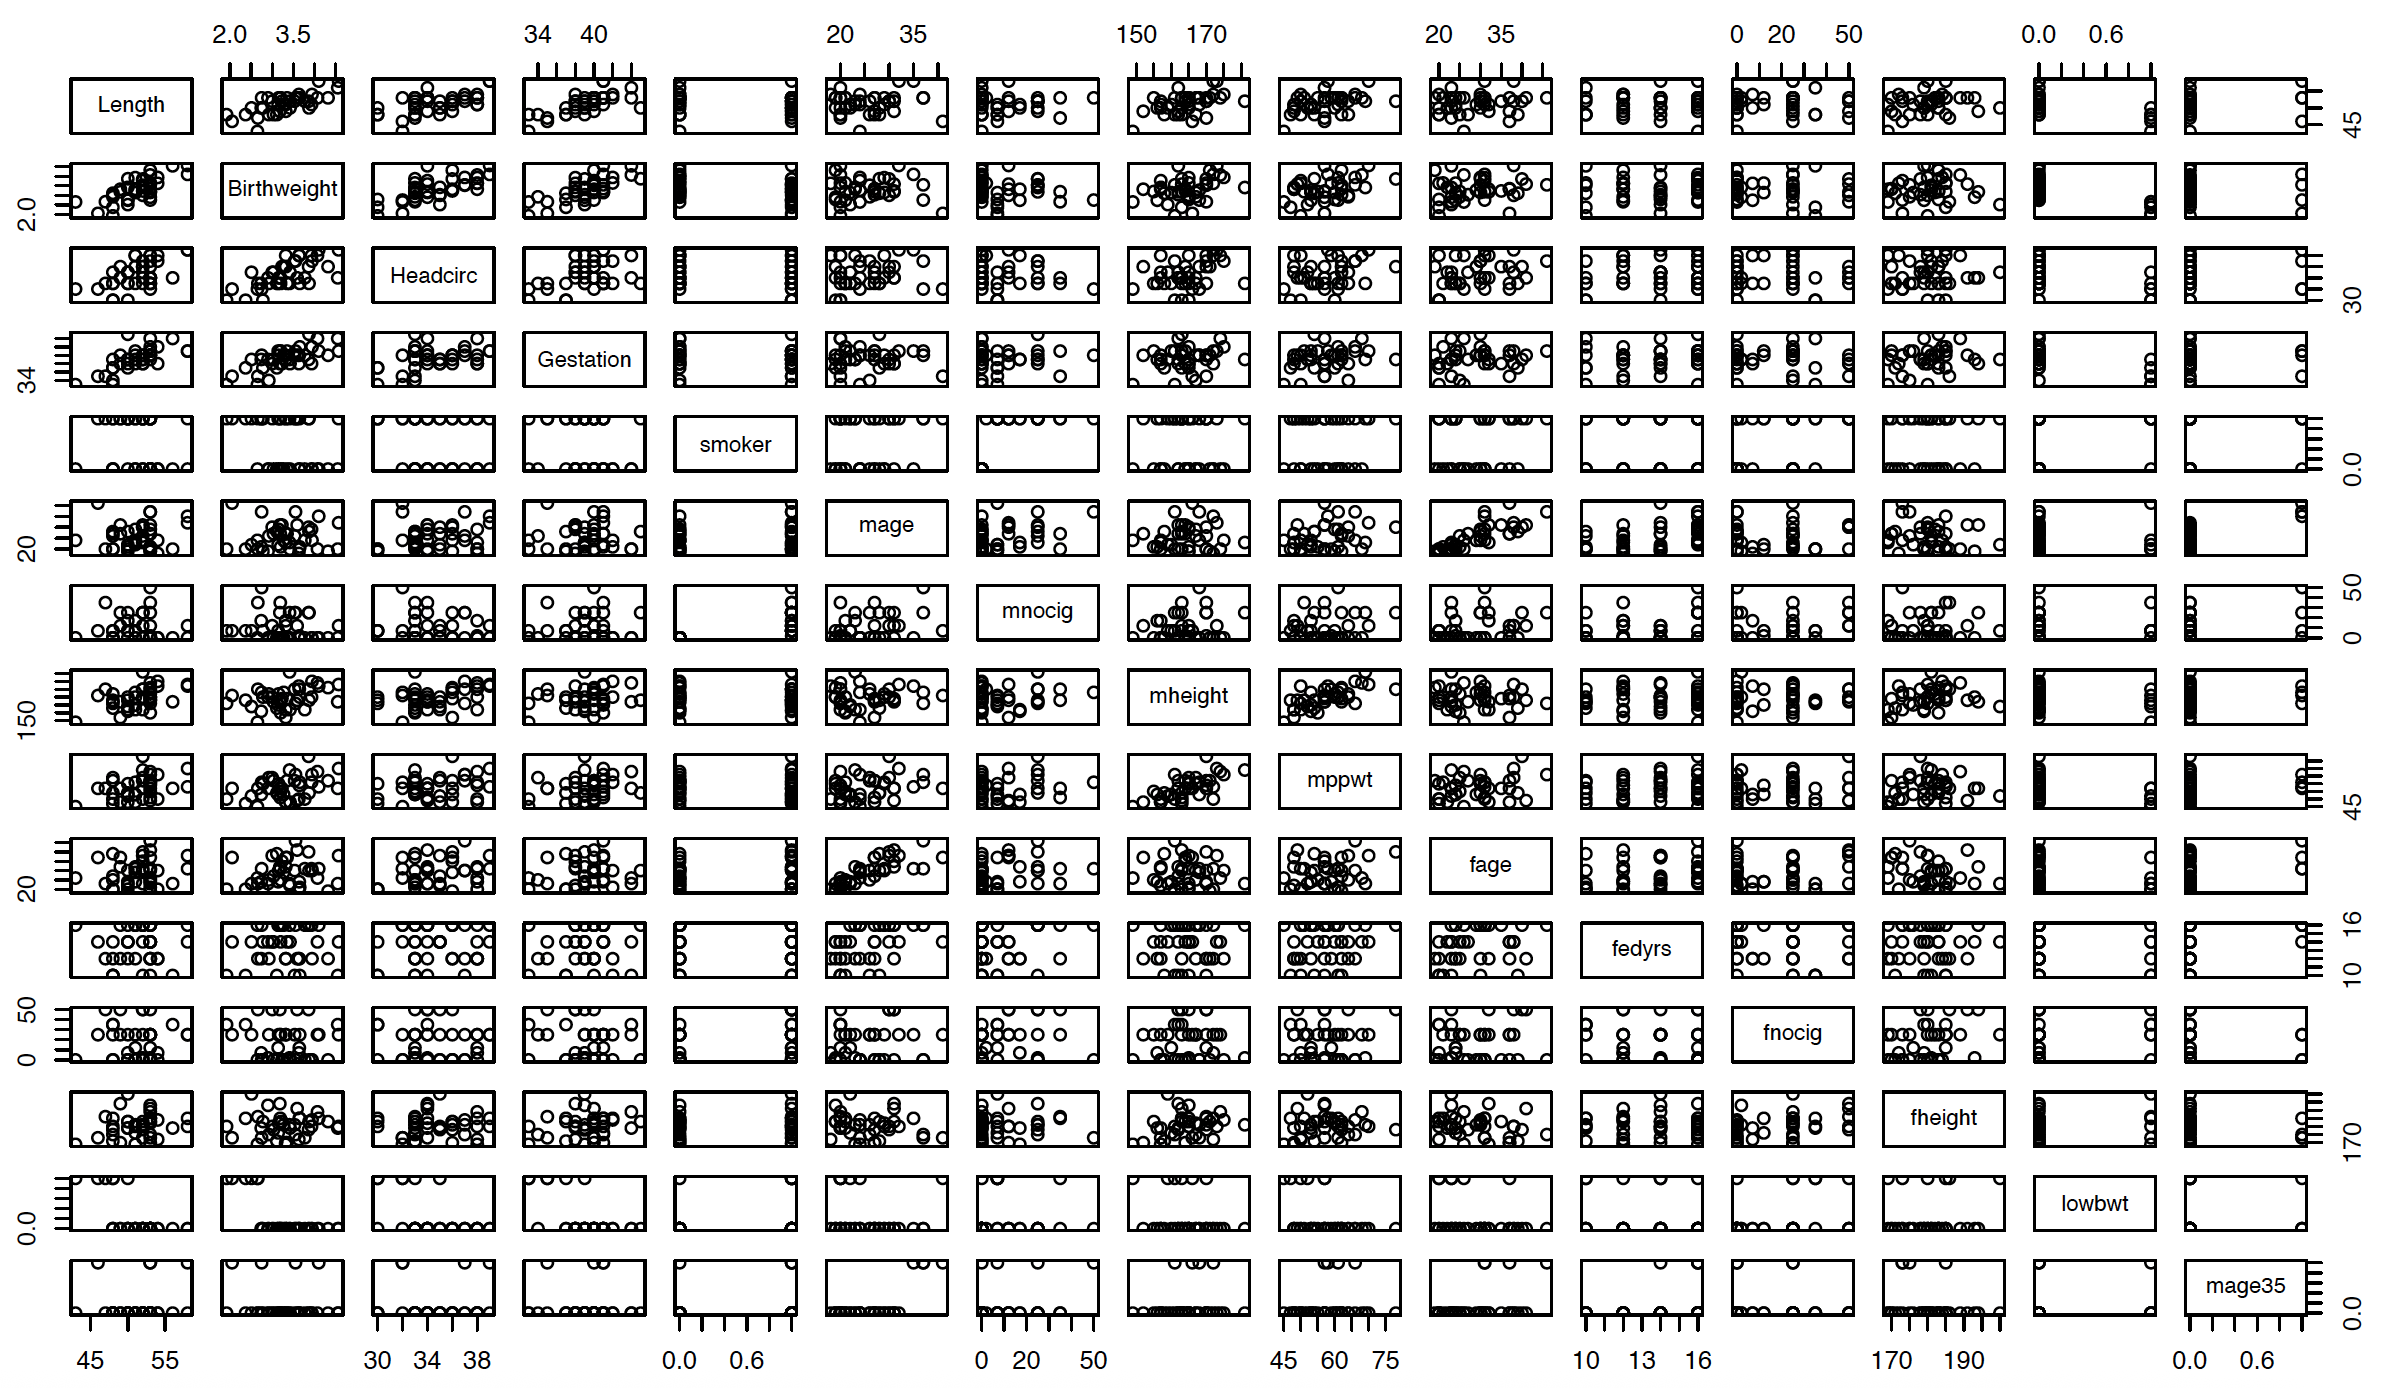
\includegraphics[width=1\linewidth]{images/week1/birthpairs} \end{center}

Note in the plots that three of the predictors, \texttt{smoker}, \texttt{lowbwt}, and \texttt{mage35} are categorical.

This is a typical example where a multiple linear regression model is a good starting point. If the fit of the model is good and all key model assumptions are satisfied, then the predictive power of this model will be strong.

\subsubsection*{\texorpdfstring{ Trees and Shrubs Data (Binary Classification) }{ Trees and Shrubs Data (Binary Classification) }}\label{trees-and-shrubs-data-binary-classification}
\addcontentsline{toc}{subsubsection}{ Trees and Shrubs Data (Binary Classification) }

In this problem, the goal is to understand whether a specific woody plan, common in the Black Forest region in Southwestern Germany (Ref: Lederer) is a tree or a shrub. A sample of the data set is shown below:

\begin{tabular}{l|r|r|r|r}
\hline
Name & Height & Diameter & GrowthRate & Longevity\\
\hline
Silver Fir & 55.0 & 1.50 & 0.5 & 500\\
\hline
European Beech & 40.0 & 1.00 & 0.5 & 200\\
\hline
Common Hazel & 5.0 & 0.10 & 0.5 & 70\\
\hline
Red Raspberry & 1.5 & 0.01 & 0.4 & 10\\
\hline
European Spruce & 50.0 & 1.20 & 0.5 & 600\\
\hline
\end{tabular}

This is a binary classification problem in which we want to use to use a set of characteristics to predict whether a specific plant is a tree or a shrub.

\subsubsection*{\texorpdfstring{ Handwritten Digits (Multiclass Classification) }{ Handwritten Digits (Multiclass Classification) }}\label{handwritten-digits-multiclass-classification}
\addcontentsline{toc}{subsubsection}{ Handwritten Digits (Multiclass Classification) }

This is a classic example of multiclass classification where the goal is to predict the handwritten digit \((0, \ldots, 9)\) from the envelope of a letter, based on a 16 \(\times\) 16 eight-bit grayscale map (Ref: ESL). The challenge in this example is to keep the error rate below a desirable threshold to avoid misdirection of mail.

\begin{center}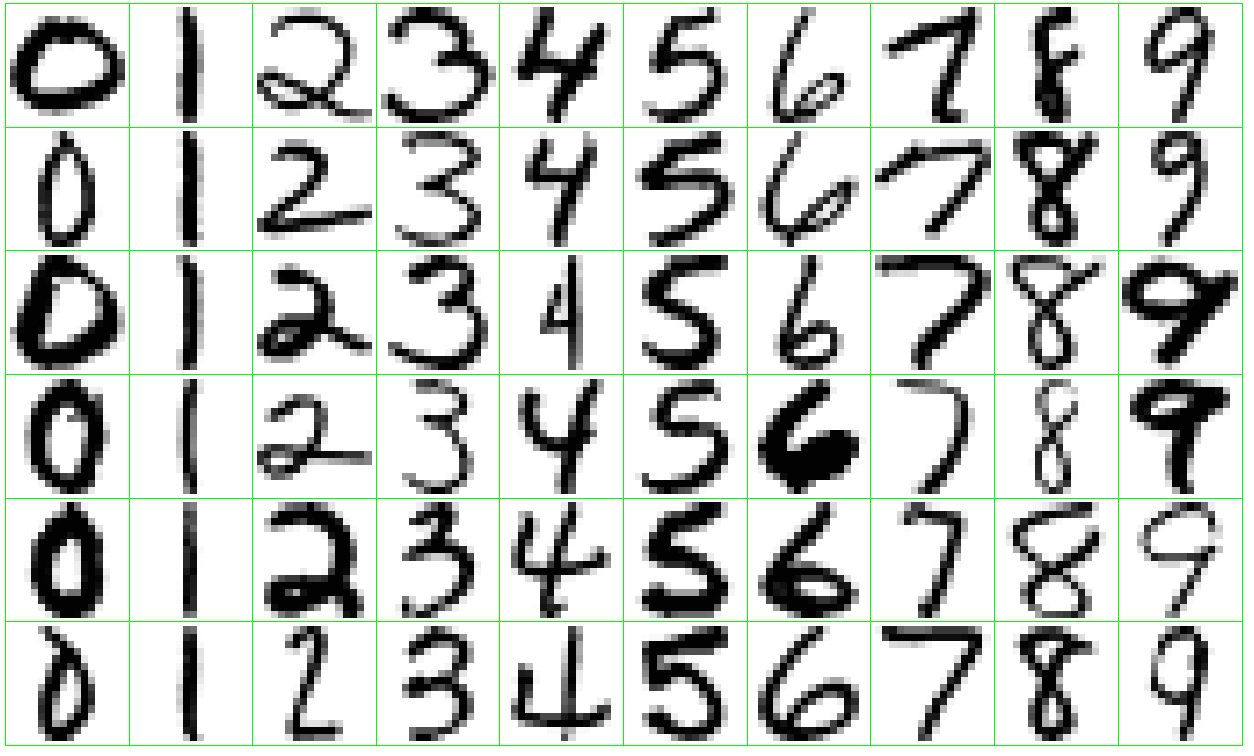
\includegraphics[width=0.75\linewidth]{images/week1/SLEx_digits} \end{center}

\subsubsection*{\texorpdfstring{ Proteomics Data (Clustering) }{ Proteomics Data (Clustering) }}\label{proteomics-data-clustering}
\addcontentsline{toc}{subsubsection}{ Proteomics Data (Clustering) }

Proteomics is the field of biology and chemistry that is focused on studying proteins in large-scale. Typically, proteomics data sets are obtained as a result of an experiment and through specific processes, such as protein purification or through mass spectrometry, a technique that is used to measure mass-to-charge ratio of ions.

In the data set below, we show the expression matrix of 437 proteins only 101 of which are of interest (Ref: Romanova et al.~-- STAT 427 dataset). The challenge in these data sets is the amount of missing data (grey pixels in the plot) and the goal is to cluster the observations into various protein groups for further analysis.

\begin{center}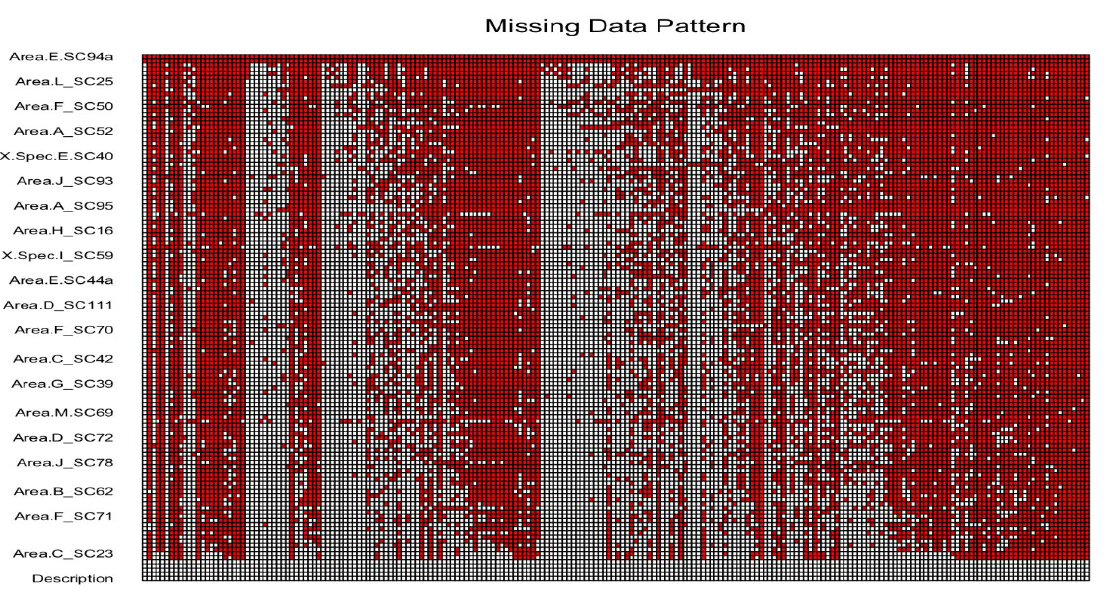
\includegraphics[width=0.85\linewidth]{images/week1/chemistry} \end{center}

\section{Supervised Learning Framework}\label{supervised-learning-framework}

In this class, our main focus is \emph{supervised learning}. This means that we have a \textbf{target}/\textbf{outcome}/\textbf{response} variable \(Y\) that we need to predict using a set of \emph{features}/\emph{predictors}, \(X\). We can assume that the relationship between the response \(Y\) and the set of features are linked via a \emph{parametric} function \(f\) as follows
\[\mathbf{y} \longleftarrow f(\mathbf{x}, w) \]
If we know the function \(f\) up to a parameter \(w\), e.g.~we know it is a linear, then our problem reduces to \textbf{learning} \(w\).

For this reason, we collect (\emph{training}) data \(\bigl\{\mathbf{x}_i, \mathbf{y}_i  \bigr\}_{i=1}^{n}\) that will help us to \emph{minimize an \textbf{objective} function} with respect to \(w\):
\[F(w) = \sum_{i=1}^{n} loss \Bigl(y_i,\, f \bigl(\mathbf{x}_i, w \bigr) \Bigr)\]
The \(loss\) function quantifies the distance between the model, i.e.~\(f(\mathbf{x}_i, w)\) and the respective outcome \(\mathbf{y}_i\). It is up to the practitioner to choose the \(loss\) function. The most popular examples are:

\begin{itemize}
\item
  the Squared Error Loss
  \[loss = \Bigl[ y_i - f\bigl(x_i; w \bigr)\Bigr]^2\]
\item
  the Absolute Error Loss
  \[loss = \Bigl| y_i - f\bigl(x_i; w \bigr)\Bigr|\]
\item
  the Log Loss
  \[loss = \begin{cases} 
  &-\log f \bigl(x_i; w \bigr), \,\, \text{ if } y_i=1\\
  &-\log \Bigl(1- f\bigl(x_i; w \bigr) \Bigr),\,\, \text{ if } y_i=0
  \end{cases} \]
\item
  the 0-1 Loss
  \[loss = \mathbf{1}_{ \left \{ y_i \neq f(x_i; w) \right\} } = \begin{cases} 
  & 1, \,\, \text{ if } y_i \neq f\bigl(x_i; w \bigr) \\
  & 0,\,\, \text{ if } y_i = f\bigl(x_i; w \bigr)
  \end{cases} \]
\end{itemize}

Depending on the choice of \(loss\) function, the minimizer of the objective function may or may not be in closed form. If not, we can try optimization algorithms that can guarantee convergence to the global minimizer. In the worst case scenario, one can always use gradient descent.

\section{Why is Statistical Learning is Challenging}\label{why-is-statistical-learning-is-challenging}

In our framework, we reduced the problem of learning, to estimating a vector of parameters. However, we assumed that we already know the true function \(f\) up to this parameter. In practice, we typically need to estimate or better \emph{approximate} the function \(f\). This approximation, denoted by \(\hat{f}\) introduces an \emph{additional source of error}.

Furthermore, in our framework we worked with a set of \emph{training} data that will be used to learn the model. The objective function quantifies the distance between the \emph{true} \(f\) parametrized by \(w\) and the observation in the training data set. However, to assess the actual performance and the predictive power of the fitted model, we need to \emph{test} it to new, unobserved data. Thus, in the statistical learning context, our goal is to minimize the \textbf{test} or \textbf{generalization error}, not the training error.

Therefore, statistical learning is a difficult task because

\begin{itemize}
\item
  the training error typically underestimates the test/generalization error.
\item
  the model performance might be good for training data, but poor for future (test) data due to overfitting.
\item
  the number of parameters needed to learn the underlying regression or classification function \(f\) might be large; and in some cases larger than the available data.
\item
  The test error increases significantly when the number of model parameters becomes larger.
\end{itemize}

Let's consider the following simple cases:

\begin{enumerate}
\def\labelenumi{(\arabic{enumi})}
\item
  In \emph{classification}, the one-nearest-neighbor approach predicts perfectly on the training data, but poorly on testing data. An interesting illustration on how dimensionality changes the performance of linear classifiers can be found here: \url{https://www.visiondummy.com/2014/04/curse-dimensionality-affect-classification/}
\item
  On the other hand, in \emph{regression}, if we take \(\mathbf{y}_{n\times 1}\) to be the regression vector, where \(n\) is the sample size, and \(\mathbf{X}_{n\times p}\) is the design matrix (i.e.~matrix of predictors) with \(p\) predictors. The underlying regression model is
  \[\mathbf{y}_{n\times 1} = \mathbf{X}_{n\times p} \, w_{p\times 1} + error\]
  where \(w_{p\times 1}\) are the model coefficients (i.e.~parameters to estimate). If
\end{enumerate}

\begin{itemize}
\item
  \(p<n\): we have \(n\) (more) equations than the \(p\) parameters; this is when typically regression methods can be successful.
\item
  \(p=n\): we have \(n\) equations and \(n\) parameters; this leads to a perfect fit on training data.
\item
  \(p>n\): we have fewer equations \(n\) than parameters \(p\): this is a scenario when classical regression methods do not perform well.
\end{itemize}

\section{Bias-Variance Trade-Off}\label{bias-variance-trade-off}

We mentioned before that we have \textbf{two sources of error} that affect the quality of the predictions we make. Specifically, we try to balance between:

\begin{itemize}
\item
  \textbf{Bias}: The bias is the difference between the estimated parameter or function and the true underlying parameter or function. High bias leads to under-fitting and an inaccurate model.
\item
  \textbf{Variance} (of an estimated function): The variance quantifies the ability of the function to ``adapt'' to small changes in the data. High variance leads to over-fitting and an unreliable model.
\end{itemize}

\begin{center}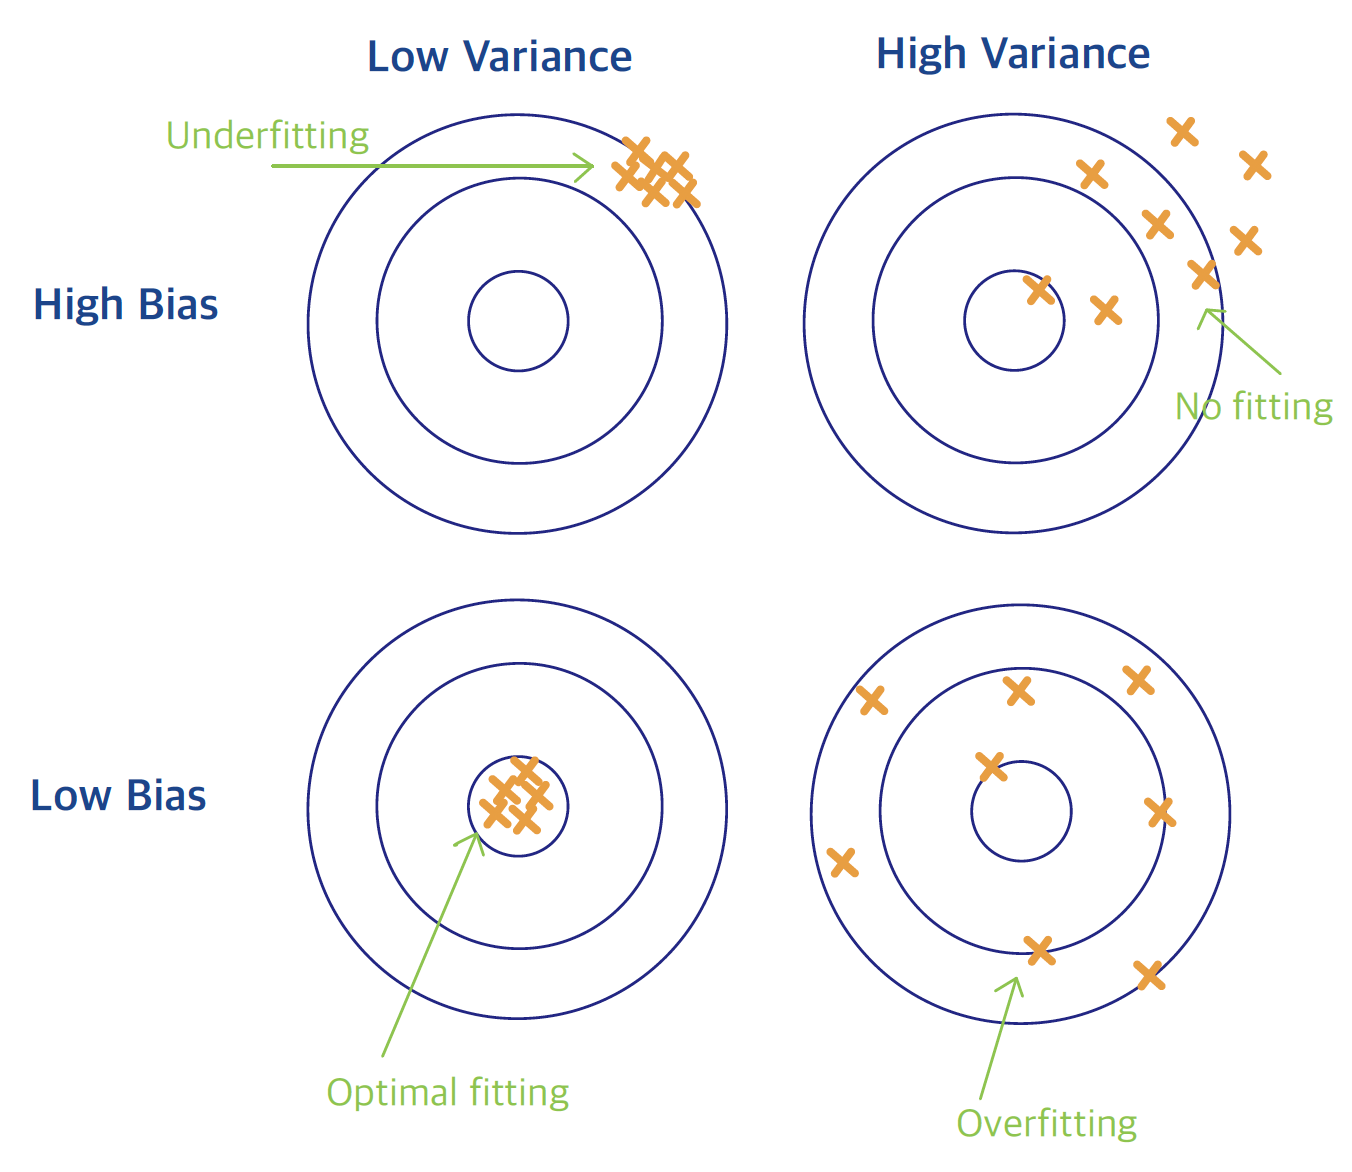
\includegraphics[width=0.6\linewidth]{images/week1/tradeoff1} \end{center}

In general, one can think of our learning problem as a \textbf{target} in which the true model lies in the center. \emph{How close to the center the fitted values are is captured by the bias}. If most of the points ``miss'' the target, then it means that our model does not approximate the true \(f\). If the bias is large, then increasing the sample size will not help us to ``hit the target''.

On the other hand, \emph{the spread of the data is measured by the variance}. If all data points are all close to each other, then the variance is low, while if they are widely spread, then the variance is high.

Ideally, we would like to minimize both variance and bias at the same time. In our context, this is not feasible which means that we need to balance between the two. Keeping in mind that in statistical learning our goal is to \emph{minimize the generalization error} --not the training error--, we can say that:

\begin{center}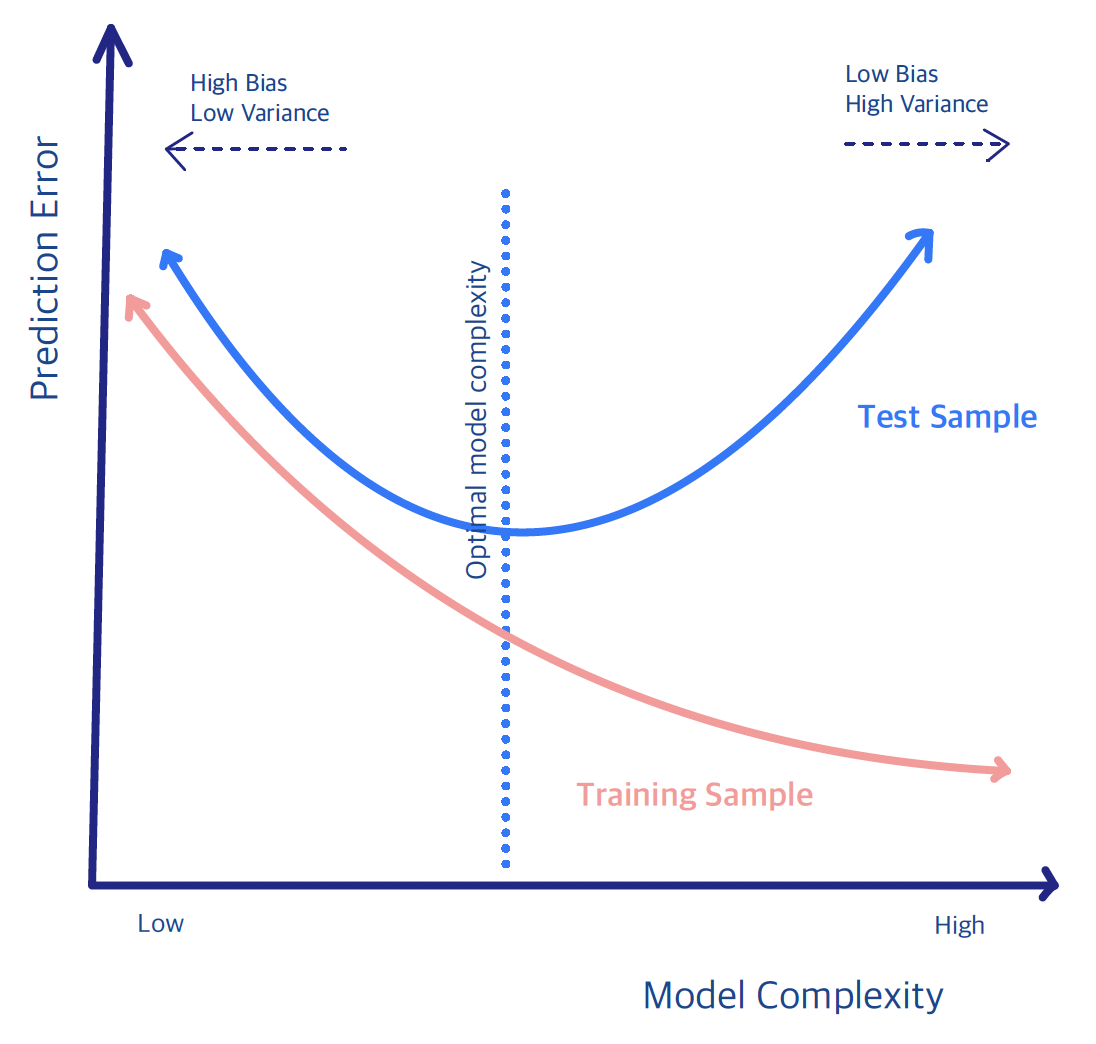
\includegraphics[width=0.5\linewidth]{images/week1/traintest2} \end{center}

\begin{itemize}
\item
  When the number of model parameters is large, or in other words when the model is complex, the prediction error in the \emph{training data} tends to \textbf{reduce}. However, when we overfit, we end up with a fitted model that follows precisely the pattern of the data and that won't generalize well, leading to a higher variance in the \emph{testing data}.
\item
  When the model is very simple, i.e.~when we have very few parameters, then it is very likely that we underfit the data, leading to larger bias and a poor generalization error.
\end{itemize}

In this class, we will discuss:

\begin{enumerate}
\def\labelenumi{(\roman{enumi})}
\item
  Flexible modeling techniques to reduce bias.
\item
  Useful strategies to achieve the trade-off between bias and variance.
\end{enumerate}

As an example, two successful approaches that balance the bias-variance trade-off that we will study are.

\begin{itemize}
\item
  \textbf{Regularization}: Restrict the parameters to a low-dimensional space, which is adaptively determined by the data.
\item
  \textbf{Ensemble}: Average many low-bias high-variance models \(\longrightarrow\) averaging reduces variance.
\end{itemize}

\section{\texorpdfstring{Two Toy Examples: \(k\)NN vs.~Linear Regression}{Two Toy Examples: kNN vs.~Linear Regression}}\label{two-toy-examples-knn-vs.-linear-regression}

Before we wrap up the introduction, we will review two simple supervised learning examples
(i) \(k\)-Nearest Neighbors (\(k\)NN)
(ii) Linear Regression\\
and will examine their performance and understand the bias-variance trade-off.

\subsection{\texorpdfstring{\(k\)-Nearest Neighbors}{k-Nearest Neighbors}}\label{k-nearest-neighbors}

In the \textbf{\(k\)-Nearest Neighbors} (\(k\)NN) method, we use observations in the training set that are closest to \(\mathbf{x}\) to form \(\mathbf{y}\). Specifically, the \(k\)-Nearest Neighbor fit for \(\hat{y}\) is
\[\hat{\mathbf{y}}(\mathbf{x}) = \frac{1}{k} \sum_{x_i \in N_k(\mathbf{x})} y_i\]
where \(N_k(\mathbf{x})\) is the neighborhood of \(\mathbf{x}\) defined by the \(k\) closest points \(x_i\) in the training sample. In a regression context the \(k\)NN fitted \(\mathbf{\hat{y}}\) predicts \(\mathbf{y}\) via a \textbf{local average}, while in the classification context \(k\)NN returns the \textbf{majority vote} in \(N_k(\mathbf{x})\) or a probability calculated on the frequencies in \(N_k(\mathbf{x})\). What can be challenging in the \(k\)NN approach is \emph{tuning} \(k\), the neighborhood size, and determining the metric to define the neighborhood.

\begin{itemize}
\item
  The choice of \(k\) is directly linked to the complexity of the method which is roughly equal to \(n/k\).

  \begin{itemize}
  \item
    When \(k=1\), the prediction at \(x_i\) is \textbf{exactly} \(y_i\) which means that we have zero training error.
  \item
    When \(k=n\), every neighborhood contains all the \(n\) training samples, so the prediction is the same no matter \(x\).
  \end{itemize}
\item
  The default metric to define the neighborhood is the \emph{Euclidean distance}:
  \[d\bigl( \mathbf{x}, \tilde{\mathbf{x}} \bigr) = \sum_{j=1}^{p} w_j \bigl( x_j - \tilde{x}_j \bigr)^2,\]
  where we would like to learn the \(w_j\)'s from the data.
\end{itemize}

\subsection{Linear Regression}\label{linear-regression}

Given a vector of inputs \(\mathbf{x}^T = (x_1, x_2, \ldots, x_p)\), we \textbf{approximate} \(Y\) via a \emph{linear} function
\[f(\mathbf{x}) \approx \beta_0 + \sum_{j=1}^{p} x_j \beta_j\]
Our goal is to \emph{estimate} the parameters \(\beta_j\) using the Least-Squares (LS) method by minimizing the Residual Sum of Squares (\emph{objective function})
\[\min_{\beta_0, \ldots, \beta_p} \sum_{i=1}^{n} \Bigl( y_i - \beta_0 - x_{i1}\beta_1 - \ldots - x_{ip} \beta_p \Bigr)^2\]
The solution is easy to obtain (both in R/Python and analytically under certain assumptions) and the fitted value for the \(i\)th input \(x_i\) is given by
\[\hat{y}_i = \hat{y}(x_i) = x_i^T \hat{\beta}\]
We leave the details to be discussed in Week 2.

\subsubsection*{Linear Regression in a Classification Context}\label{linear-regression-in-a-classification-context}
\addcontentsline{toc}{subsubsection}{Linear Regression in a Classification Context}

We can apply linear regression on classification problems with \(Y=0 \text{ or } 1\). In this case, we predict \(Y\) to be 1 if the LS prediction \(f(x)\) is bigger than 0.5, and 0 otherwise. This approach has drawbacks. First of all, the squared difference \(p(\mathbf{x}) = \Bigl(y_i - f(\mathbf{x}_i) \Bigr)^2\) is not a good evaluation metric, since considering a linear function \(f(\mathbf{x})\) may result in values outside \([0,1]\). Therefore, when we are in this context a Logistic regression is the gold standard according to which
\[\log \frac{p(\mathbf{x})}{1-p(\mathbf{x}) } \approx \beta_0 + \sum_{j=1}^{p} x_j \beta_j\]

More on this in Week 8.

\subsection{Simulated Binary Classification Example}\label{simulated-binary-classification-example}

Consider a response variable \(G\) that takes two values (0 -- BLUE or 1 -- ORANGE). In our simulation, we generate 200 such values; 100 in each class, and our goal is to use both regression and \(k\)NN to classify the data. The code behind the simulation and the plots can be found here.

We start by fitting a linear regression model to the simulated data. In a naive approach, we treat the response is a continuous variable. Hence, the continuous fitted values \(\hat{Y}\) are converted to a fitted class variable \(\hat{G}\) according to the following rule:
\[\hat{G} = \begin{cases}
& Blue, \text{ if } \hat{Y} > 0.5\\
& Orange, \text{ otherwise } \\
\end{cases} \]

Our classification example is in two dimensions which means that the decision boundary (the boundary that separates the orange from the blue region) is a straight line.

\begin{center}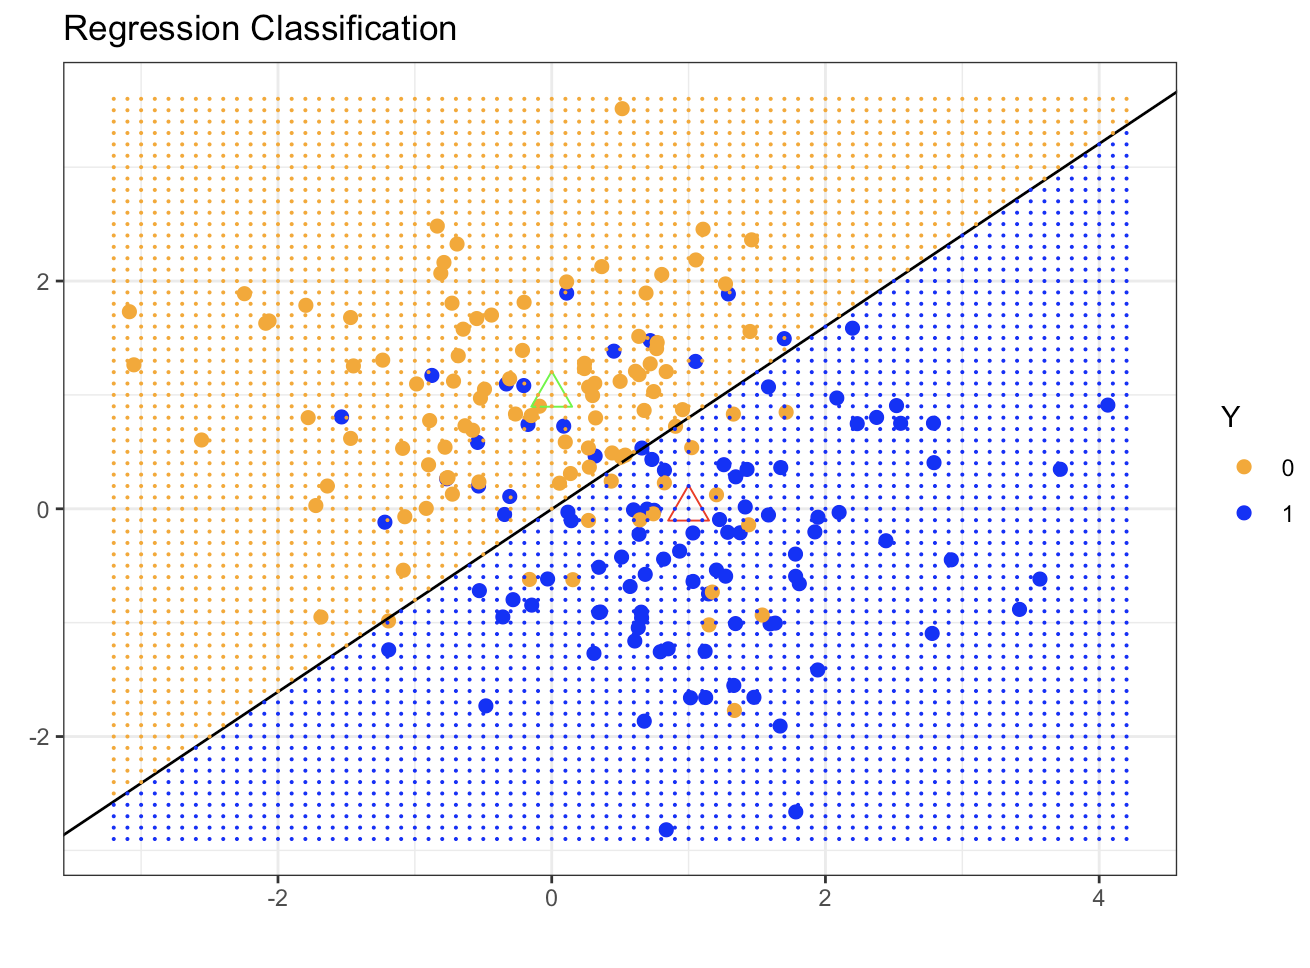
\includegraphics[width=0.7\linewidth]{images/week1/regclass} \end{center}

Specifically, the fitted decision boundary is a straight line (the black line in the plot) defined by \(\mathbf{x}^T \hat{\beta} = 0.5\). Based on our simulation, we know that the blue region should be above the black fitted regression line, while the orange region should be below the black fitted regression line. We observe that there are many misclassifications on both sides of the decision boundary.

The regression line seems to be very smooth and too rigid when it comes to classifying the data. On the other end of the spectrum, we have the \(k\) Nearest-Neighbor approach. So, for the same simulated data, the nearest neighbor method will use the observations in the training set closest in input space to \(X\) to form \(\hat{Y}\).

Using a 15-nearest-neighbor averaging of the binary coded response such that \(\hat{Y}\) is the proportion of blue's in the neighborhood, then we assign
\[\hat{G} = \begin{cases}
& Blue, \text{ if } \hat{Y} > 0.5\\
& Orange,\text{ otherwise } \\
\end{cases} \]

In this case, the predicted class is chosen by majority vote amont the 15 nearest neighbors.

\begin{center}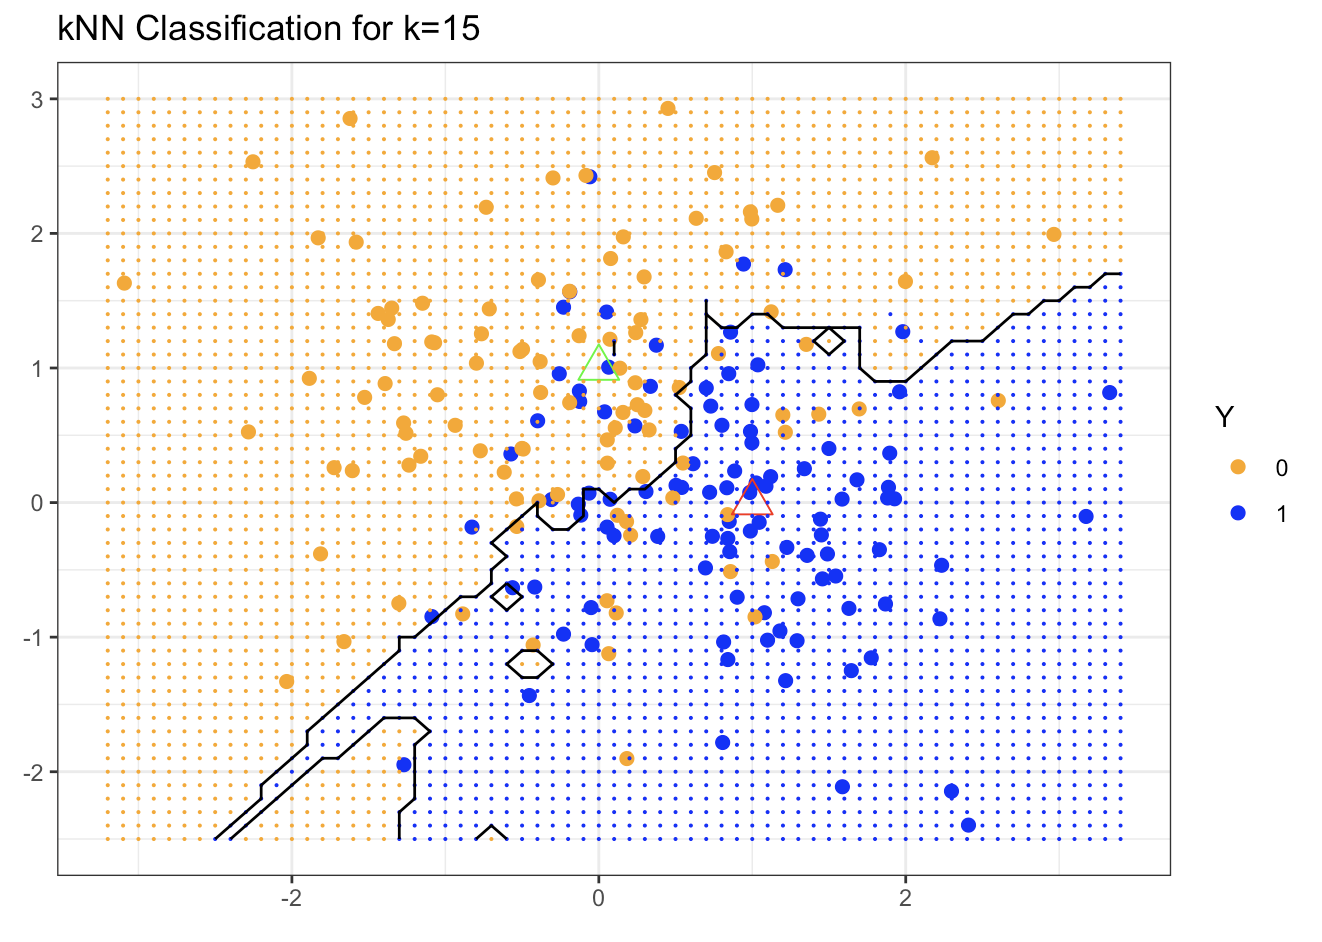
\includegraphics[width=0.7\linewidth]{images/week1/kNN15} \end{center}

We observe that the decision boundary separating the blue from the orange region is far more irregular than before and sensitive to local clusters of blue and orange dots. As a result, we have fewer misclassified observations than before. Remember that we can tune the neighborhood size. So, if we take the extreme scenario in which \(k=1\) and we only consider \textbf{one} neighbor, we have

\begin{center}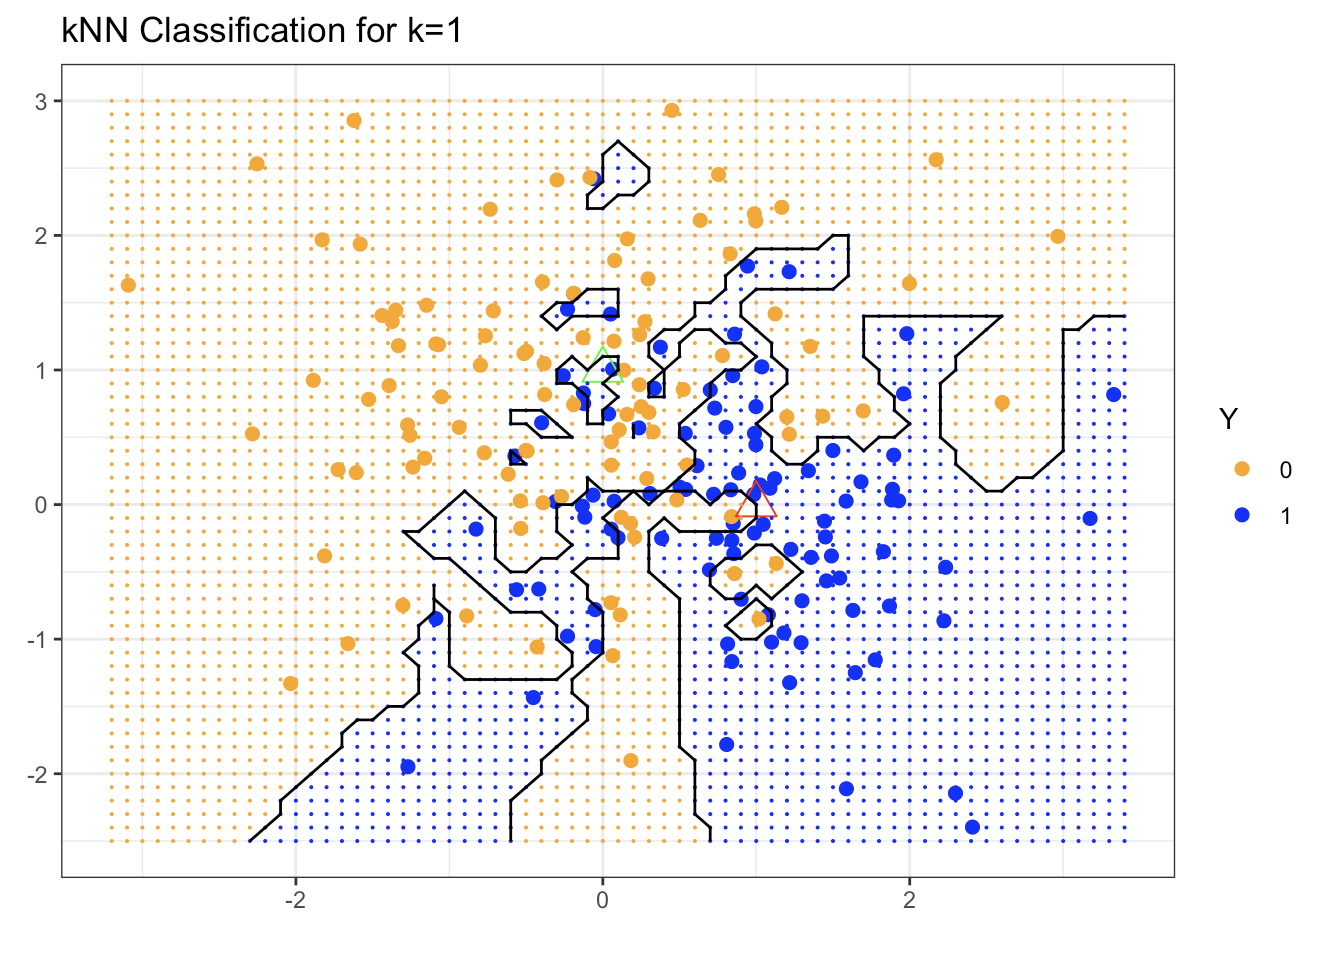
\includegraphics[width=0.7\linewidth]{images/week1/kNN1} \end{center}

This results in a much rougher decision boundary with hardly any misclassified data. However, is this the ideal choice? The answer is no, but in order to understand the reason we need to consider the \emph{generalization error}.

Up to now, we have used the same data for training and comparison purposes. As a result, a method like \(k\)NN has seemingly 0 error for \(k=1\). In order to make fair comparisons, we should consider another data set, independent of the one used to fit the data, so that we can compute the test/generalization error for both methods.

In the plot below, we compare the misclassification error on the testing data set as a function of the degrees of freedom. In other words, we compare several \(k\)NN fits (for different \(k\)s) and the regression fit. The testing set here contains 10,000 observations.

\begin{center}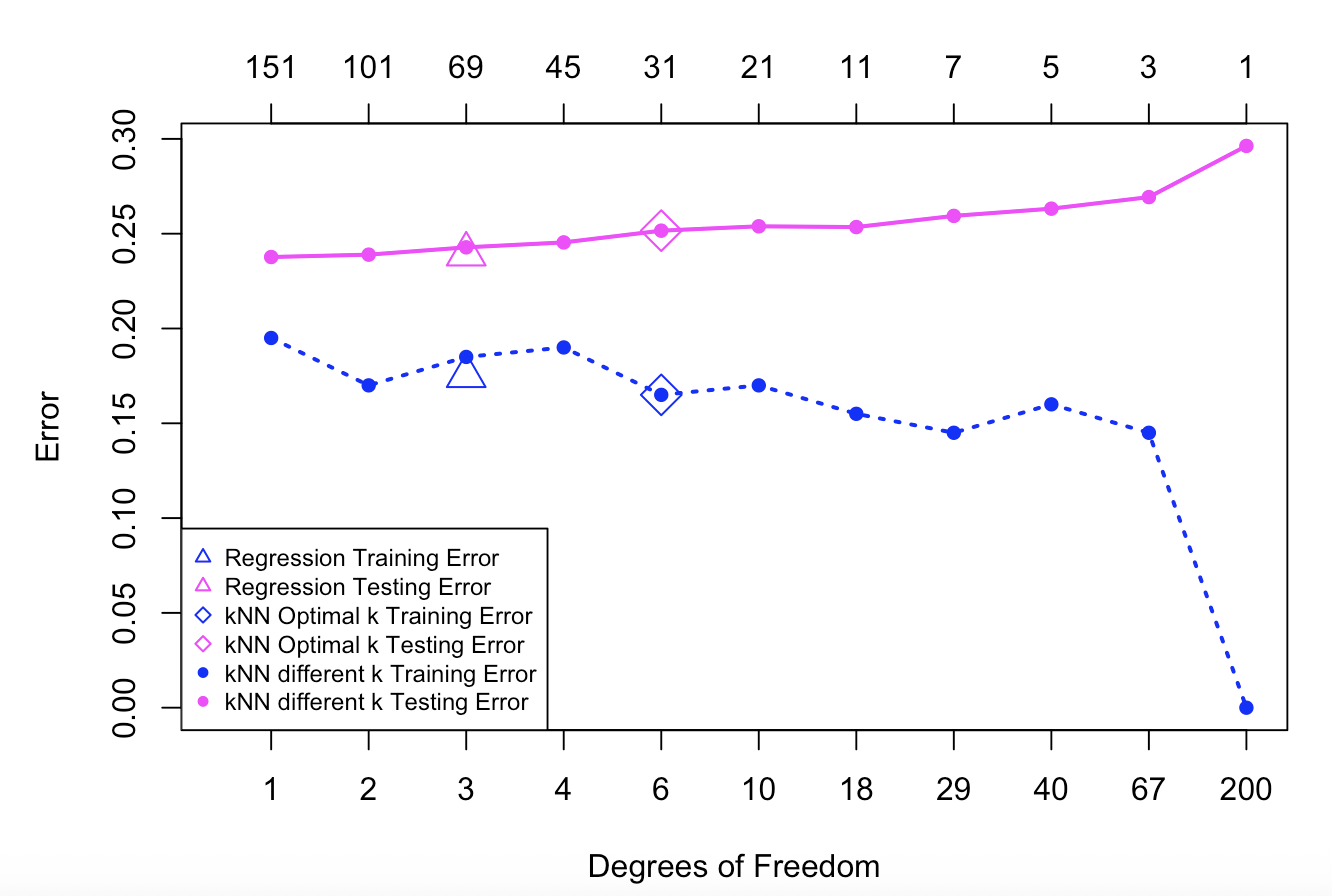
\includegraphics[width=0.7\linewidth]{images/week1/traintesterror} \end{center}

The magenta curve is the test error and the blue curve is the training error for the \(k\)NN classification for different \(k\)s. In our simulated example, we used a 5-fold cross validation method to identify the optimal \(k\). The results for the optimal \(k\) in \(k\)NN are denoted with a diamond. The results for linear regression are the
magenta and blue triangles at 3 DFs (the DFs were determined based on the dimension of the linear model we fitted).

The regression method has the advantage of it being linear with only \(p=3\) parameters to estimate which means that it has a relatively \emph{low variance}. However, the linearity assumption seems to be quite restrictive for the classification problem under consideration, which means that we expect to have high bias.

On the other hand, the \(k\)NN approach has no assumption of the shape of the underlying \(f\), maybe except some local smoothness. This flexibility results in overfitting and a low bias (we saw that in the extreme case of \(k=1\)).It can be shown that as \(k, n \rightarrow \infty\) such that \(k/n \rightarrow 0\), \(k\)NN is consistent. At the same time, the method has higher variance with the extreme case of when the number of parameters for \(k\)NN is roughly \(n=k\), which goes to \(\infty\) in order to achieve consistency.

\subsection{Code for the Examples in the Lectures}\label{code-for-the-examples-in-the-lectures}

We replicate one of the examples in the ESL book to illustrate the differences between the two simplest prediction methods for binary outcomes: the \emph{Regression method} and the \emph{\(k\)-Nearest-Neighbors method}.

\subsubsection{Simulation}\label{simulation}

\begin{itemize}
\tightlist
\item
  The \emph{generated data} consist of a \textbf{binary classification} with two classes, labeled as \texttt{0} and \texttt{1}.
\item
  The \emph{features} are two-dimensional.
\item
  \texttt{Class\ 1} data points are generated from a Gaussian distribution with mean \(\mu_1\) and variance \(\sigma^2\), i.e.~\(X_{1,1}, \ldots, X_{1,n_1} \sim \mathbb{N}\bigl( \mu_1, \sigma^2 \bigr)\).
\item
  \texttt{Class\ 0} data points are generated from a Gaussian distribution with mean \(\mu_2\) and variance \(\sigma^2\),i.e.~\(X_{01}, \ldots, X_{0n_2} \sim \mathbb{N}\bigl( \mu_0, \sigma^2 \bigr)\).
\item
  In total, we generate \emph{200 training samples} (\(n=100\) for each class), and we assign labels to the training data (100 \texttt{Class\ 1} and 100 \texttt{Class\ 0}).
\item
  Similarly, we generate \emph{10,000 test samples}.
\end{itemize}

\subsubsection{Code for the Simulation}\label{code-for-the-simulation}

Set the model parameters for the simulation:

\begin{Shaded}
\begin{Highlighting}[]
\NormalTok{p }\OtherTok{=} \DecValTok{2}\NormalTok{;           }\DocumentationTok{\#\# No. of parameters}
\NormalTok{sigma }\OtherTok{=} \DecValTok{1}\NormalTok{;       }\DocumentationTok{\#\# St. Dev for the Normals (common)}
\NormalTok{mu1 }\OtherTok{=} \FunctionTok{c}\NormalTok{(}\DecValTok{1}\NormalTok{, }\DecValTok{0}\NormalTok{);   }\DocumentationTok{\#\# Vector of means for the first Normal}
\NormalTok{mu0 }\OtherTok{=} \FunctionTok{c}\NormalTok{(}\DecValTok{0}\NormalTok{, }\DecValTok{1}\NormalTok{);   }\DocumentationTok{\#\# Vector of means for the second Normal}
\end{Highlighting}
\end{Shaded}

Generate \(n\) i.i.d. (independent and identically distributed) samples from each normal to create the \emph{training} data set.

\begin{Shaded}
\begin{Highlighting}[]
\NormalTok{n }\OtherTok{=} \DecValTok{100}\NormalTok{;         }\DocumentationTok{\#\# Training Sample Size for each Normal}

\DocumentationTok{\#\# rnorm(2*n*p) generates 2*n*p  N(0,1) random variables.}
\DocumentationTok{\#\# matrix(rnorm(2*n*p), 2*n, p)*sigma generates a 2n{-}by{-}p matrix of two N(0, sigma\^{}2) each of length 2*n.}
\DocumentationTok{\#\# Adding matrix(rep(mu1, n), nrow=n,byrow=TRUE) to each column of the previous matrix}
\DocumentationTok{\#\#    shifts each of the columns to generate the Normals with means mu1 or mu0.}
\DocumentationTok{\#\# Note that both mu0, mu1 are 2{-}dimensional.}

\NormalTok{traindata }\OtherTok{=} \FunctionTok{matrix}\NormalTok{(}\FunctionTok{rnorm}\NormalTok{(}\DecValTok{2}\SpecialCharTok{*}\NormalTok{n}\SpecialCharTok{*}\NormalTok{p), }\DecValTok{2}\SpecialCharTok{*}\NormalTok{n, p)}\SpecialCharTok{*}\NormalTok{sigma }\SpecialCharTok{+} 
            \FunctionTok{rbind}\NormalTok{(}\FunctionTok{matrix}\NormalTok{(}\FunctionTok{rep}\NormalTok{(mu1, n), }\AttributeTok{nrow=}\NormalTok{n,}\AttributeTok{byrow=}\ConstantTok{TRUE}\NormalTok{), }
            \FunctionTok{matrix}\NormalTok{(}\FunctionTok{rep}\NormalTok{(mu0, n), }\AttributeTok{nrow=}\NormalTok{n, }\AttributeTok{byrow=}\ConstantTok{TRUE}\NormalTok{))}

\CommentTok{\# dim(traindata)}

\DocumentationTok{\#\# We generate the 0 or 1 labels.}
\NormalTok{Ytrain }\OtherTok{=} \FunctionTok{factor}\NormalTok{(}\FunctionTok{c}\NormalTok{(}\FunctionTok{rep}\NormalTok{(}\DecValTok{1}\NormalTok{,n), }\FunctionTok{rep}\NormalTok{(}\DecValTok{0}\NormalTok{,n)))}
\end{Highlighting}
\end{Shaded}

Generate \(N\) \emph{test} samples in a similar way:

\begin{Shaded}
\begin{Highlighting}[]
\NormalTok{N}\OtherTok{=}\DecValTok{10000}\NormalTok{;  }

\NormalTok{testdata }\OtherTok{=} \FunctionTok{matrix}\NormalTok{(}\FunctionTok{rnorm}\NormalTok{(}\DecValTok{2}\SpecialCharTok{*}\NormalTok{N}\SpecialCharTok{*}\NormalTok{p), }\DecValTok{2}\SpecialCharTok{*}\NormalTok{N, p)}\SpecialCharTok{*}\NormalTok{sigma}\SpecialCharTok{+} 
           \FunctionTok{rbind}\NormalTok{(}\FunctionTok{matrix}\NormalTok{(}\FunctionTok{rep}\NormalTok{(mu1, N), }\AttributeTok{nrow=}\NormalTok{N,}\AttributeTok{byrow=}\ConstantTok{TRUE}\NormalTok{), }
           \FunctionTok{matrix}\NormalTok{(}\FunctionTok{rep}\NormalTok{(mu0, N), }\AttributeTok{nrow=}\NormalTok{N, }\AttributeTok{byrow=}\ConstantTok{TRUE}\NormalTok{))}

\NormalTok{Ytest }\OtherTok{=} \FunctionTok{factor}\NormalTok{(}\FunctionTok{c}\NormalTok{(}\FunctionTok{rep}\NormalTok{(}\DecValTok{1}\NormalTok{,N), }\FunctionTok{rep}\NormalTok{(}\DecValTok{0}\NormalTok{,N)))}
\end{Highlighting}
\end{Shaded}

\subsubsection{Visualization of the Simulated Data}\label{visualization-of-the-simulated-data}

\emph{This section also serves as a review of plotting in R.}

We visualize the data we generated -- those in the \texttt{traindata} matrix.

In the figure generated by the code below, points from two groups are colored in orange and blue, respectively; the two centers are plotted as +, and a legend is added to explain the association of each color.

\subsubsection{Using the default R functions for plotting}\label{using-the-default-r-functions-for-plotting}

\begin{Shaded}
\begin{Highlighting}[]
\DocumentationTok{\#\# Create an empty plotting area: The axes are the two vectors of normals generated, }
\DocumentationTok{\#\# each one saved in a column of the \textasciigrave{}traindata\textasciigrave{} matrix.}
\DocumentationTok{\#\# The following line creates an empty plot, since we used the option type="n"}
\DocumentationTok{\#\# We do this so that we can color{-}code the data.}
\FunctionTok{plot}\NormalTok{(traindata[,}\DecValTok{1}\NormalTok{], traindata[,}\DecValTok{2}\NormalTok{], }\AttributeTok{type=}\StringTok{"n"}\NormalTok{, }\AttributeTok{xlab=}\StringTok{""}\NormalTok{, }\AttributeTok{ylab=}\StringTok{""}\NormalTok{);}

\CommentTok{\# Add the "Class 1" points {-} in blue color.}
\FunctionTok{points}\NormalTok{(traindata[}\DecValTok{1}\SpecialCharTok{:}\NormalTok{n, }\DecValTok{1}\NormalTok{], traindata[}\DecValTok{1}\SpecialCharTok{:}\NormalTok{n,}\DecValTok{2}\NormalTok{], }\AttributeTok{pch=}\DecValTok{16}\NormalTok{, }\AttributeTok{col=}\StringTok{"blue"}\NormalTok{);}

\CommentTok{\# Add the "Class 0" points {-} in orange color}
\FunctionTok{points}\NormalTok{(traindata[(n}\SpecialCharTok{+}\DecValTok{1}\NormalTok{)}\SpecialCharTok{:}\NormalTok{(}\DecValTok{2}\SpecialCharTok{*}\NormalTok{n),}\DecValTok{1}\NormalTok{], traindata[(n}\SpecialCharTok{+}\DecValTok{1}\NormalTok{)}\SpecialCharTok{:}\NormalTok{(}\DecValTok{2}\SpecialCharTok{*}\NormalTok{n),}\DecValTok{2}\NormalTok{], }\AttributeTok{pch=}\DecValTok{16}\NormalTok{, }\AttributeTok{col=}\StringTok{"orange"}\NormalTok{); }

\CommentTok{\# Add the  centers for class 1}
\FunctionTok{points}\NormalTok{(mu1[}\DecValTok{1}\NormalTok{], mu1[}\DecValTok{2}\NormalTok{], }\AttributeTok{pch=}\DecValTok{13}\NormalTok{, }\AttributeTok{cex=}\FloatTok{1.5}\NormalTok{, }\AttributeTok{col=}\StringTok{"green"}\NormalTok{);    }

\CommentTok{\# Add the  centers for class 0}
\FunctionTok{points}\NormalTok{(mu0[}\DecValTok{1}\NormalTok{], mu0[}\DecValTok{2}\NormalTok{], }\AttributeTok{pch=}\DecValTok{13}\NormalTok{, }\AttributeTok{cex=}\FloatTok{1.5}\NormalTok{, }\AttributeTok{col=}\StringTok{"red"}\NormalTok{);   }

\FunctionTok{legend}\NormalTok{(}\StringTok{"bottomright"}\NormalTok{, }\AttributeTok{pch =} \FunctionTok{c}\NormalTok{(}\DecValTok{16}\NormalTok{,}\DecValTok{16}\NormalTok{), }\AttributeTok{col =} \FunctionTok{c}\NormalTok{(}\StringTok{"blue"}\NormalTok{, }\StringTok{"orange"}\NormalTok{), }
       \AttributeTok{legend =} \FunctionTok{c}\NormalTok{(}\StringTok{"Class 1"}\NormalTok{, }\StringTok{"Class 0"}\NormalTok{))}
\end{Highlighting}
\end{Shaded}

\pandocbounded{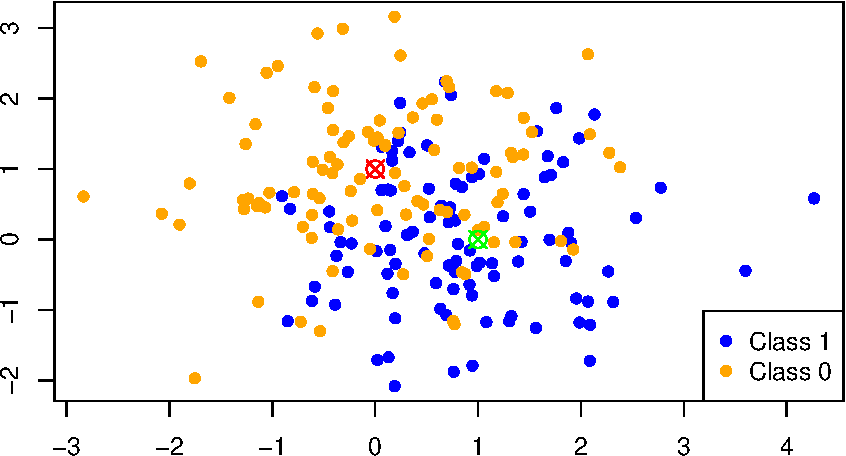
\includegraphics[keepaspectratio]{_main_files/figure-latex/unnamed-chunk-15-1.pdf}}

\subsubsection{\texorpdfstring{Using the \texttt{ggplot2} R library}{Using the ggplot2 R library}}\label{using-the-ggplot2-r-library}

In this section, we present an alternative way to construct the plot above via the \texttt{ggplot2} package. The \texttt{ggplot2} package allows us to create elaborate plots. More information can be found here: \url{http://ggplot2.org/}

\begin{Shaded}
\begin{Highlighting}[]
\CommentTok{\# install.package("ggplot2")}
\FunctionTok{library}\NormalTok{(}\StringTok{"ggplot2"}\NormalTok{)}

\DocumentationTok{\#\# The input in a \textasciigrave{}ggplot\textasciigrave{} function can only be a data.frame}

\DocumentationTok{\#\# In our case the data is a matrix, so we convert them to data.frames here:}
\NormalTok{mytraindata }\OtherTok{=} \FunctionTok{data.frame}\NormalTok{(}\AttributeTok{X1=}\NormalTok{traindata[,}\DecValTok{1}\NormalTok{], }\AttributeTok{X2=}\NormalTok{traindata[,}\DecValTok{2}\NormalTok{], }\AttributeTok{Y=}\NormalTok{Ytrain)}

\DocumentationTok{\#\# The ggplot output is an object which is saved in training.scatter.}
\DocumentationTok{\#\# In this object, we can later add {-}{-}and plot{-}{-} additional features.}

\NormalTok{training.scatter }\OtherTok{=} \FunctionTok{ggplot}\NormalTok{(mytraindata, }\FunctionTok{aes}\NormalTok{(X1, X2)) }\SpecialCharTok{+}  \DocumentationTok{\#\# creates the empty plot}
        \FunctionTok{geom\_point}\NormalTok{(}\FunctionTok{aes}\NormalTok{(}\AttributeTok{colour=}\NormalTok{Y), }\AttributeTok{size=}\DecValTok{2}\NormalTok{) }\SpecialCharTok{+} \DocumentationTok{\#\# adds the points color{-}coded by the labels in Y}
        \FunctionTok{scale\_color\_manual}\NormalTok{(}\AttributeTok{values =} \FunctionTok{c}\NormalTok{(}\StringTok{"orange"}\NormalTok{, }\StringTok{"blue"}\NormalTok{)) }\SpecialCharTok{+}  \DocumentationTok{\#\# change the default colors}
        \DocumentationTok{\#\# Use geom\_point to add the centers (as before)}
        \FunctionTok{geom\_point}\NormalTok{(}\AttributeTok{data=}\FunctionTok{data.frame}\NormalTok{(}\AttributeTok{X1=}\NormalTok{mu1[}\DecValTok{1}\NormalTok{], }\AttributeTok{X2=}\NormalTok{mu1[}\DecValTok{2}\NormalTok{]), }\FunctionTok{aes}\NormalTok{(X1, X2), }\AttributeTok{colour=}\StringTok{"green"}\NormalTok{, }\AttributeTok{shape=}\DecValTok{2}\NormalTok{,}\AttributeTok{size=}\DecValTok{5}\NormalTok{) }\SpecialCharTok{+}
        \FunctionTok{geom\_point}\NormalTok{(}\AttributeTok{data=}\FunctionTok{data.frame}\NormalTok{(}\AttributeTok{X1=}\NormalTok{mu0[}\DecValTok{1}\NormalTok{], }\AttributeTok{X2=}\NormalTok{mu0[}\DecValTok{2}\NormalTok{]), }\FunctionTok{aes}\NormalTok{(X1, X2), }\AttributeTok{colour=}\StringTok{"red"}\NormalTok{, }\AttributeTok{shape=}\DecValTok{2}\NormalTok{, }\AttributeTok{size=}\DecValTok{5}\NormalTok{) }\SpecialCharTok{+}
        \FunctionTok{ggtitle}\NormalTok{(}\StringTok{"Simulated Training Data"}\NormalTok{)  }\SpecialCharTok{+} \DocumentationTok{\#\# add a title }
        \FunctionTok{labs}\NormalTok{(}\AttributeTok{x =} \StringTok{""}\NormalTok{, }\AttributeTok{y=}\StringTok{""}\NormalTok{)  }\DocumentationTok{\#\# remove axes labels}
  
\FunctionTok{plot}\NormalTok{(training.scatter)}
\end{Highlighting}
\end{Shaded}

\pandocbounded{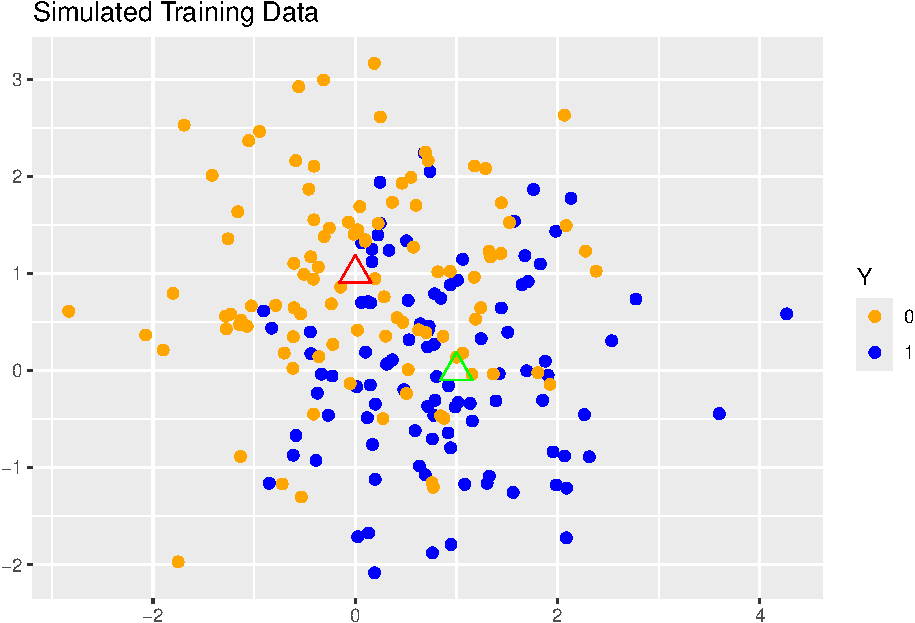
\includegraphics[keepaspectratio]{_main_files/figure-latex/unnamed-chunk-16-1.pdf}}

\subsubsection{\texorpdfstring{\(k\) Nearest-Neighbors Method}{k Nearest-Neighbors Method}}\label{k-nearest-neighbors-method}

To apply the \(k\)-NN method, we need to choose \(k\). In the example below, we use the neighborhood sizes suggested from the textbook (ESL). We also apply and plot the results for \(k=1\) and \(k=15\).

\begin{Shaded}
\begin{Highlighting}[]
\FunctionTok{library}\NormalTok{(}\StringTok{"class"}\NormalTok{) }

\NormalTok{neighbor\_size }\OtherTok{=} \FunctionTok{c}\NormalTok{(}\DecValTok{151}\NormalTok{, }\DecValTok{101}\NormalTok{, }\DecValTok{69}\NormalTok{,  }\DecValTok{45}\NormalTok{, }\DecValTok{31}\NormalTok{, }\DecValTok{21}\NormalTok{, }\DecValTok{11}\NormalTok{, }\DecValTok{7}\NormalTok{, }\DecValTok{5}\NormalTok{, }\DecValTok{3}\NormalTok{, }\DecValTok{1}\NormalTok{); }\DocumentationTok{\#\# These are different k\textquotesingle{}s to try.}
\NormalTok{m }\OtherTok{=} \FunctionTok{length}\NormalTok{(neighbor\_size);  }\DocumentationTok{\#\# needed to run our for{-}loop below.}

\NormalTok{train.err.knn }\OtherTok{=} \FunctionTok{rep}\NormalTok{(}\DecValTok{0}\NormalTok{,m);   }\DocumentationTok{\#\# vector to store training error}
\NormalTok{test.err.knn }\OtherTok{=} \FunctionTok{rep}\NormalTok{(}\DecValTok{0}\NormalTok{, m);   }\DocumentationTok{\#\# vector to store testing error}

\DocumentationTok{\#\# knn is the R function that runs the kNN method. Output is a factor.}

\ControlFlowTok{for}\NormalTok{( j }\ControlFlowTok{in} \DecValTok{1}\SpecialCharTok{:}\NormalTok{m)\{}
\NormalTok{  Ytrain.pred }\OtherTok{=} \FunctionTok{knn}\NormalTok{(traindata, traindata, Ytrain, }\AttributeTok{k=}\NormalTok{neighbor\_size[j])   }\DocumentationTok{\#\# predictions for training data}
\NormalTok{  train.err.knn[j]}\OtherTok{=} \FunctionTok{sum}\NormalTok{(Ytrain }\SpecialCharTok{!=}\NormalTok{ Ytrain.pred)}\SpecialCharTok{/}\NormalTok{(}\DecValTok{2}\SpecialCharTok{*}\NormalTok{n)     }\DocumentationTok{\#\# mis{-}classification training error}
\NormalTok{  Ytest.pred }\OtherTok{=} \FunctionTok{knn}\NormalTok{(traindata, testdata, Ytrain,}\AttributeTok{k=}\NormalTok{neighbor\_size[j])      }\DocumentationTok{\#\# predictions for testing data}
\NormalTok{  test.err.knn[j] }\OtherTok{=} \FunctionTok{sum}\NormalTok{(Ytest }\SpecialCharTok{!=}\NormalTok{ Ytest.pred)}\SpecialCharTok{/}\NormalTok{(}\DecValTok{2}\SpecialCharTok{*}\NormalTok{N)       }\DocumentationTok{\#\# mis{-}classification testing error}
\NormalTok{\}}

\FunctionTok{cbind}\NormalTok{(train.err.knn, test.err.knn)    }\DocumentationTok{\#\# matrix containing the train and test errors}
\end{Highlighting}
\end{Shaded}

\begin{verbatim}
##       train.err.knn test.err.knn
##  [1,]         0.285      0.24085
##  [2,]         0.270      0.24110
##  [3,]         0.265      0.24180
##  [4,]         0.280      0.24630
##  [5,]         0.280      0.25185
##  [6,]         0.305      0.25690
##  [7,]         0.255      0.27030
##  [8,]         0.235      0.27565
##  [9,]         0.220      0.28590
## [10,]         0.160      0.30210
## [11,]         0.000      0.31735
\end{verbatim}

\subsubsection{\texorpdfstring{5-Fold Cross-Validation for Choosing optimal \(k\)}{5-Fold Cross-Validation for Choosing optimal k}}\label{fold-cross-validation-for-choosing-optimal-k}

A systematic way to determine the \emph{optimal} value for the neighborhood size, \(k\), in a range of values is the so-called 5-fold Cross-Validation (CV) method. Essentially, the method selects the \(k\) value that minimizes the CV error. In a nutshell, the 5-fold CV error for each \(k\) is a \emph{sum of 5 prediction errors}, one corresponding to each fold.

In the code below, we have an outside loop from 1 to 5 (the folds), and an inside loop from 1 to \(m\) (all possible values for \(k\)). Inside the loop, we use 80\% (i.e., four folds) of the data as training and predict on the 20\% (i.e., one fold) holdout set.

\begin{Shaded}
\begin{Highlighting}[]
\DocumentationTok{\#\# In this chunk of code, we use the same vector of k\textquotesingle{}s as above {-} the neighbor\_size vector of size m}

\DocumentationTok{\#\# Initialize a vector cv.error to store the CV error for each k.}
\NormalTok{cv.error }\OtherTok{=} \FunctionTok{rep}\NormalTok{(}\DecValTok{0}\NormalTok{,m);}


\NormalTok{id }\OtherTok{=} \FunctionTok{sample}\NormalTok{(}\DecValTok{1}\SpecialCharTok{:}\NormalTok{(}\DecValTok{2}\SpecialCharTok{*}\NormalTok{n),(}\DecValTok{2}\SpecialCharTok{*}\NormalTok{n), }\AttributeTok{replace=}\ConstantTok{FALSE}\NormalTok{);}
\NormalTok{fold }\OtherTok{=} \FunctionTok{c}\NormalTok{(}\DecValTok{0}\NormalTok{,  }\DecValTok{40}\NormalTok{,  }\DecValTok{80}\NormalTok{, }\DecValTok{120}\NormalTok{, }\DecValTok{160}\NormalTok{, }\DecValTok{200}\NormalTok{)}

\ControlFlowTok{for}\NormalTok{(i }\ControlFlowTok{in} \DecValTok{1}\SpecialCharTok{:}\DecValTok{5}\NormalTok{)}
    \ControlFlowTok{for}\NormalTok{(j }\ControlFlowTok{in} \DecValTok{1}\SpecialCharTok{:}\NormalTok{m)\{}
      
      \DocumentationTok{\#\# ith.fold = rows which are in the i{-}th fold}
\NormalTok{      ith.fold }\OtherTok{=}\NormalTok{ id[(fold[i]}\SpecialCharTok{+}\DecValTok{1}\NormalTok{)}\SpecialCharTok{:}\NormalTok{fold[i}\SpecialCharTok{+}\DecValTok{1}\NormalTok{]];   }
\NormalTok{      tmp }\OtherTok{=} \FunctionTok{knn}\NormalTok{(traindata[}\SpecialCharTok{{-}}\NormalTok{ith.fold,], traindata[ith.fold,], Ytrain[}\SpecialCharTok{{-}}\NormalTok{ith.fold], }\AttributeTok{k=}\NormalTok{neighbor\_size[j]);}
\NormalTok{      cv.error[j]}\OtherTok{=}\NormalTok{cv.error[j] }\SpecialCharTok{+} \FunctionTok{sum}\NormalTok{(tmp }\SpecialCharTok{!=}\NormalTok{ Ytrain[ith.fold])}
\NormalTok{    \}}

\DocumentationTok{\#\# Find the optimal k value based 5{-}fold CV}
\NormalTok{k.optimal }\OtherTok{=}\NormalTok{ neighbor\_size[}\FunctionTok{order}\NormalTok{(cv.error)[}\DecValTok{1}\NormalTok{]]  }

\DocumentationTok{\#\# Error of KNN for the k is chosen by 5{-}fold CV}
\NormalTok{Ytrain.pred }\OtherTok{=} \FunctionTok{knn}\NormalTok{(traindata, traindata, Ytrain, }\AttributeTok{k=}\NormalTok{k.optimal)}
\NormalTok{train.err.knn.CV }\OtherTok{=} \FunctionTok{sum}\NormalTok{(Ytrain }\SpecialCharTok{!=}\NormalTok{ Ytrain.pred)}\SpecialCharTok{/}\NormalTok{(}\DecValTok{2}\SpecialCharTok{*}\NormalTok{n)}
\NormalTok{Ytest.pred }\OtherTok{=} \FunctionTok{knn}\NormalTok{(traindata, testdata, Ytrain,}\AttributeTok{k=}\NormalTok{k.optimal)}
\NormalTok{test.err.knn.CV }\OtherTok{=} \FunctionTok{sum}\NormalTok{(Ytest }\SpecialCharTok{!=}\NormalTok{ Ytest.pred)}\SpecialCharTok{/}\NormalTok{(}\DecValTok{2}\SpecialCharTok{*}\NormalTok{N)  }
\end{Highlighting}
\end{Shaded}

\subsubsection{Least Squares Method}\label{least-squares-method}

We run a regression of \texttt{Ytrain} vs.~the \texttt{traindata}, and we classify the results as follows:
\[\hat{Y} = \begin{cases} & 1, \text{ if } fitted(Y) > 0.5\\
                          & 0, \text{ if } fitted(Y) \leq 0.5
            \end{cases} \]

\begin{Shaded}
\begin{Highlighting}[]
\DocumentationTok{\#\# Run a regression using the lm function}
\DocumentationTok{\#\# Ytrain is a factor, so we need to convert it to a numeric vector to run the lm}
\NormalTok{RegModel }\OtherTok{=} \FunctionTok{lm}\NormalTok{(}\FunctionTok{as.numeric}\NormalTok{(Ytrain)}\SpecialCharTok{{-}}\DecValTok{1} \SpecialCharTok{\textasciitilde{}}\NormalTok{ traindata)}

\DocumentationTok{\#\# Compute the \textbackslash{}hat\{Y\} for training }
\NormalTok{Ytrain\_pred\_LS }\OtherTok{=} \FunctionTok{as.numeric}\NormalTok{(RegModel}\SpecialCharTok{$}\NormalTok{fitted }\SpecialCharTok{\textgreater{}} \FloatTok{0.5}\NormalTok{)}

\DocumentationTok{\#\# Compute the predicted values for testing data and then the \textbackslash{}hat\{Y\}}
\NormalTok{Ytest\_pred\_LS }\OtherTok{=}\NormalTok{ RegModel}\SpecialCharTok{$}\NormalTok{coef[}\DecValTok{1}\NormalTok{] }\SpecialCharTok{+}\NormalTok{ RegModel}\SpecialCharTok{$}\NormalTok{coef[}\DecValTok{2}\NormalTok{] }\SpecialCharTok{*}\NormalTok{ testdata[,}\DecValTok{1}\NormalTok{] }\SpecialCharTok{+}\NormalTok{ RegModel}\SpecialCharTok{$}\NormalTok{coef[}\DecValTok{3}\NormalTok{] }\SpecialCharTok{*}\NormalTok{ testdata[,}\DecValTok{2}\NormalTok{]}
\NormalTok{Ytest\_pred\_LS }\OtherTok{=} \FunctionTok{as.numeric}\NormalTok{(Ytest\_pred\_LS }\SpecialCharTok{\textgreater{}} \FloatTok{0.5}\NormalTok{ )}


\DocumentationTok{\#\# Cross{-}tab for training data and training error}
\FunctionTok{table}\NormalTok{(Ytrain, Ytrain\_pred\_LS);   }
\end{Highlighting}
\end{Shaded}

\begin{verbatim}
##       Ytrain_pred_LS
## Ytrain  0  1
##      0 70 30
##      1 26 74
\end{verbatim}

\begin{Shaded}
\begin{Highlighting}[]
\NormalTok{train.err.LS }\OtherTok{=} \FunctionTok{sum}\NormalTok{(Ytrain }\SpecialCharTok{!=}\NormalTok{  Ytrain\_pred\_LS) }\SpecialCharTok{/}\NormalTok{ (}\DecValTok{2}\SpecialCharTok{*}\NormalTok{n);  }

\DocumentationTok{\#\# Cross{-}tab for test data and test error}
\FunctionTok{table}\NormalTok{(Ytest, Ytest\_pred\_LS);     }
\end{Highlighting}
\end{Shaded}

\begin{verbatim}
##      Ytest_pred_LS
## Ytest    0    1
##     0 7638 2362
##     1 2359 7641
\end{verbatim}

\begin{Shaded}
\begin{Highlighting}[]
\NormalTok{test.err.LS }\OtherTok{=} \FunctionTok{sum}\NormalTok{(Ytest }\SpecialCharTok{!=}\NormalTok{  Ytest\_pred\_LS) }\SpecialCharTok{/}\NormalTok{ (}\DecValTok{2}\SpecialCharTok{*}\NormalTok{N);}
\end{Highlighting}
\end{Shaded}

\subsubsection{Illustration of the Results}\label{illustration-of-the-results}

First, we illustrate the classification achieved by each method.

\subsubsection{kNN Classification for two k's: k = 15 and k = 1}\label{knn-classification-for-two-ks-k-15-and-k-1}

\begin{Shaded}
\begin{Highlighting}[]
\DocumentationTok{\#\# Grid Using kNN Classification: We first define the boundaries for the grid}

\NormalTok{x.min }\OtherTok{=} \FunctionTok{round}\NormalTok{(}\FunctionTok{min}\NormalTok{(mytraindata}\SpecialCharTok{$}\NormalTok{X1), }\AttributeTok{digits=}\DecValTok{1}\NormalTok{)}\SpecialCharTok{{-}}\FloatTok{0.1}
\NormalTok{x.max }\OtherTok{=} \FunctionTok{round}\NormalTok{(}\FunctionTok{max}\NormalTok{(mytraindata}\SpecialCharTok{$}\NormalTok{X1), }\AttributeTok{digits=}\DecValTok{1}\NormalTok{)}\SpecialCharTok{+}\FloatTok{0.1}
\NormalTok{y.min }\OtherTok{=} \FunctionTok{round}\NormalTok{(}\FunctionTok{min}\NormalTok{(mytraindata}\SpecialCharTok{$}\NormalTok{X2), }\AttributeTok{digits=}\DecValTok{1}\NormalTok{)}\SpecialCharTok{{-}}\FloatTok{0.1}
\NormalTok{y.max }\OtherTok{=} \FunctionTok{round}\NormalTok{(}\FunctionTok{max}\NormalTok{(mytraindata}\SpecialCharTok{$}\NormalTok{X2), }\AttributeTok{digits=}\DecValTok{1}\NormalTok{)}\SpecialCharTok{+}\FloatTok{0.1}
\NormalTok{x.range }\OtherTok{=} \FunctionTok{seq}\NormalTok{(}\AttributeTok{from=}\NormalTok{x.min, }\AttributeTok{to=}\NormalTok{x.max, }\AttributeTok{by=}\FloatTok{0.1}\NormalTok{)}
\NormalTok{y.range }\OtherTok{=} \FunctionTok{seq}\NormalTok{(}\AttributeTok{from=}\NormalTok{y.min, }\AttributeTok{to=}\NormalTok{y.max, }\AttributeTok{by=}\FloatTok{0.1}\NormalTok{)}
\NormalTok{x.new }\OtherTok{=} \FunctionTok{expand.grid}\NormalTok{(x.range, y.range)}
\FunctionTok{names}\NormalTok{(x.new) }\OtherTok{=} \FunctionTok{names}\NormalTok{(mytraindata[,}\SpecialCharTok{{-}}\DecValTok{3}\NormalTok{])}

\DocumentationTok{\#\# Basic scatterplot (same as before): }
\DocumentationTok{\#\#   this is used as a base to add the boundary and shaded areas}

\NormalTok{grid.plot }\OtherTok{=}  \FunctionTok{ggplot}\NormalTok{(mytraindata, }\FunctionTok{aes}\NormalTok{(X1, X2)) }\SpecialCharTok{+}
            \FunctionTok{geom\_point}\NormalTok{(}\FunctionTok{aes}\NormalTok{(}\AttributeTok{colour=}\NormalTok{Y), }\AttributeTok{size=}\DecValTok{2}\NormalTok{) }\SpecialCharTok{+} 
            \FunctionTok{scale\_color\_manual}\NormalTok{(}\AttributeTok{values =} \FunctionTok{c}\NormalTok{(}\StringTok{"orange"}\NormalTok{, }\StringTok{"blue"}\NormalTok{))   }\SpecialCharTok{+}
            \FunctionTok{geom\_point}\NormalTok{(}\AttributeTok{data=}\FunctionTok{data.frame}\NormalTok{(}\AttributeTok{X1=}\NormalTok{mu1[}\DecValTok{1}\NormalTok{], }\AttributeTok{X2=}\NormalTok{mu1[}\DecValTok{2}\NormalTok{]), }\FunctionTok{aes}\NormalTok{(X1, X2), }\AttributeTok{colour=}\StringTok{"red"}\NormalTok{, }\AttributeTok{shape=}\DecValTok{2}\NormalTok{,}\AttributeTok{size=}\DecValTok{5}\NormalTok{) }\SpecialCharTok{+}
            \FunctionTok{geom\_point}\NormalTok{(}\AttributeTok{data=}\FunctionTok{data.frame}\NormalTok{(}\AttributeTok{X1=}\NormalTok{mu0[}\DecValTok{1}\NormalTok{], }\AttributeTok{X2=}\NormalTok{mu0[}\DecValTok{2}\NormalTok{]), }\FunctionTok{aes}\NormalTok{(X1, X2), }\AttributeTok{colour=}\StringTok{"green"}\NormalTok{, }\AttributeTok{shape=}\DecValTok{2}\NormalTok{, }\AttributeTok{size=}\DecValTok{5}\NormalTok{) }\SpecialCharTok{+}
            \FunctionTok{labs}\NormalTok{(}\AttributeTok{x =} \StringTok{""}\NormalTok{, }\AttributeTok{y=}\StringTok{""}\NormalTok{)}


\DocumentationTok{\#\# Plot for k=15}

\NormalTok{knn.yhat}\FloatTok{.15} \OtherTok{=} \FunctionTok{knn}\NormalTok{(traindata, x.new, Ytrain,  }\AttributeTok{k=}\DecValTok{15}\NormalTok{) }
\NormalTok{knn.pred}\FloatTok{.15} \OtherTok{=} \FunctionTok{ifelse}\NormalTok{(}\FunctionTok{as.numeric}\NormalTok{(knn.yhat}\FloatTok{.15}\NormalTok{)}\SpecialCharTok{\textgreater{}}\FloatTok{0.5}\NormalTok{,}\StringTok{"1"}\NormalTok{,}\StringTok{"0"}\NormalTok{)}

\NormalTok{knn.plotdata}\FloatTok{.15} \OtherTok{=} \FunctionTok{as.data.frame}\NormalTok{(}\FunctionTok{cbind}\NormalTok{(x.new, knn.yhat}\FloatTok{.15}\NormalTok{))}


\NormalTok{knn.plot}\FloatTok{.15} \OtherTok{=}\NormalTok{ grid.plot }\SpecialCharTok{+} 
            \FunctionTok{theme\_bw}\NormalTok{() }\SpecialCharTok{+} \CommentTok{\#remove grey background}
            \FunctionTok{geom\_point}\NormalTok{(}\AttributeTok{data=}\NormalTok{knn.plotdata}\FloatTok{.15}\NormalTok{, }\FunctionTok{aes}\NormalTok{(}\AttributeTok{x=}\NormalTok{X1, }\AttributeTok{y=}\NormalTok{X2, }\AttributeTok{colour=}\NormalTok{knn.yhat}\FloatTok{.15}\NormalTok{), }\AttributeTok{size=}\FloatTok{0.05}\NormalTok{) }\SpecialCharTok{+}
            \FunctionTok{geom\_contour}\NormalTok{(}\AttributeTok{data=}\NormalTok{knn.plotdata}\FloatTok{.15}\NormalTok{, }\FunctionTok{aes}\NormalTok{(}\AttributeTok{x=}\NormalTok{X1, }\AttributeTok{y=}\NormalTok{X2, }\AttributeTok{z=}\FunctionTok{as.numeric}\NormalTok{(knn.yhat}\FloatTok{.15}\NormalTok{)), }\AttributeTok{bins=}\DecValTok{1}\NormalTok{, }\AttributeTok{color=}\StringTok{"black"}\NormalTok{)}\SpecialCharTok{+}
            \FunctionTok{ggtitle}\NormalTok{(}\StringTok{"kNN Classification for k=15"}\NormalTok{) }

\FunctionTok{plot}\NormalTok{(knn.plot}\FloatTok{.15}\NormalTok{)}
\end{Highlighting}
\end{Shaded}

\pandocbounded{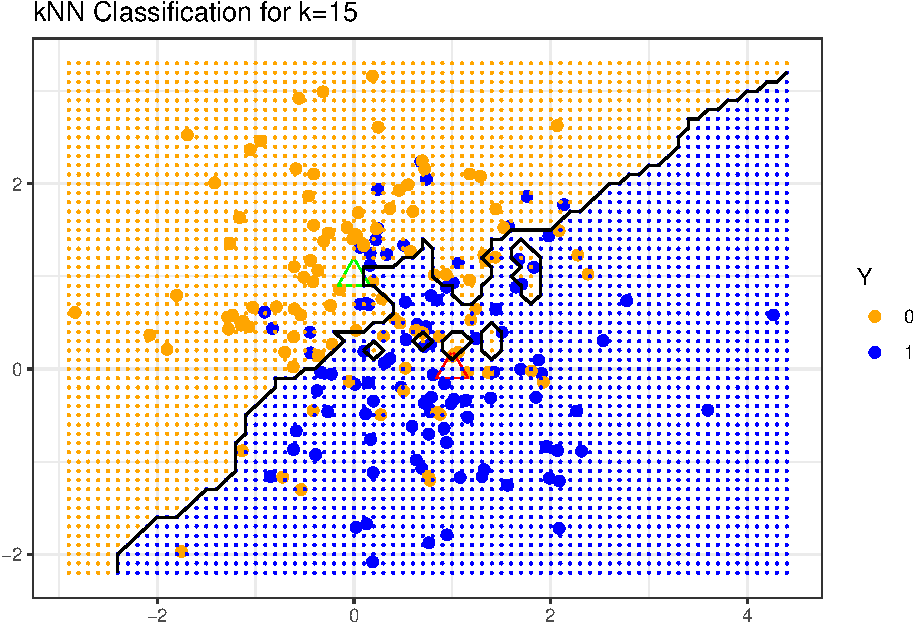
\includegraphics[keepaspectratio]{_main_files/figure-latex/unnamed-chunk-20-1.pdf}}

\begin{Shaded}
\begin{Highlighting}[]
\DocumentationTok{\#\# Plot for k=1}

\NormalTok{knn.yhat}\FloatTok{.1} \OtherTok{=} \FunctionTok{knn}\NormalTok{(traindata, x.new, Ytrain,  }\AttributeTok{k=}\DecValTok{1}\NormalTok{) }
\NormalTok{knn.pred}\FloatTok{.1} \OtherTok{=} \FunctionTok{ifelse}\NormalTok{(}\FunctionTok{as.numeric}\NormalTok{(knn.yhat}\FloatTok{.1}\NormalTok{)}\SpecialCharTok{\textgreater{}}\FloatTok{0.5}\NormalTok{, }\StringTok{"1"}\NormalTok{, }\StringTok{"0"}\NormalTok{)}

\NormalTok{knn.plotdata}\FloatTok{.1} \OtherTok{=} \FunctionTok{as.data.frame}\NormalTok{(}\FunctionTok{cbind}\NormalTok{(x.new, knn.yhat}\FloatTok{.1}\NormalTok{))}


\NormalTok{knn.plot}\FloatTok{.1} \OtherTok{=}\NormalTok{ grid.plot }\SpecialCharTok{+} 
            \FunctionTok{theme\_bw}\NormalTok{() }\SpecialCharTok{+} 
            \FunctionTok{geom\_point}\NormalTok{(}\AttributeTok{data=}\NormalTok{knn.plotdata}\FloatTok{.1}\NormalTok{, }\FunctionTok{aes}\NormalTok{(}\AttributeTok{x=}\NormalTok{X1, }\AttributeTok{y=}\NormalTok{X2, }\AttributeTok{colour=}\NormalTok{knn.yhat}\FloatTok{.1}\NormalTok{), }\AttributeTok{size=}\FloatTok{0.05}\NormalTok{) }\SpecialCharTok{+}
            \FunctionTok{geom\_contour}\NormalTok{(}\AttributeTok{data=}\NormalTok{knn.plotdata}\FloatTok{.1}\NormalTok{, }\FunctionTok{aes}\NormalTok{(}\AttributeTok{x=}\NormalTok{X1, }\AttributeTok{y=}\NormalTok{X2, }\AttributeTok{z=}\FunctionTok{as.numeric}\NormalTok{(knn.yhat}\FloatTok{.1}\NormalTok{)), }\AttributeTok{bins=}\DecValTok{1}\NormalTok{, }\AttributeTok{color=}\StringTok{"black"}\NormalTok{)}\SpecialCharTok{+}
            \FunctionTok{ggtitle}\NormalTok{(}\StringTok{"kNN Classification for k=1"}\NormalTok{) }

\FunctionTok{plot}\NormalTok{(knn.plot}\FloatTok{.1}\NormalTok{)}
\end{Highlighting}
\end{Shaded}

\pandocbounded{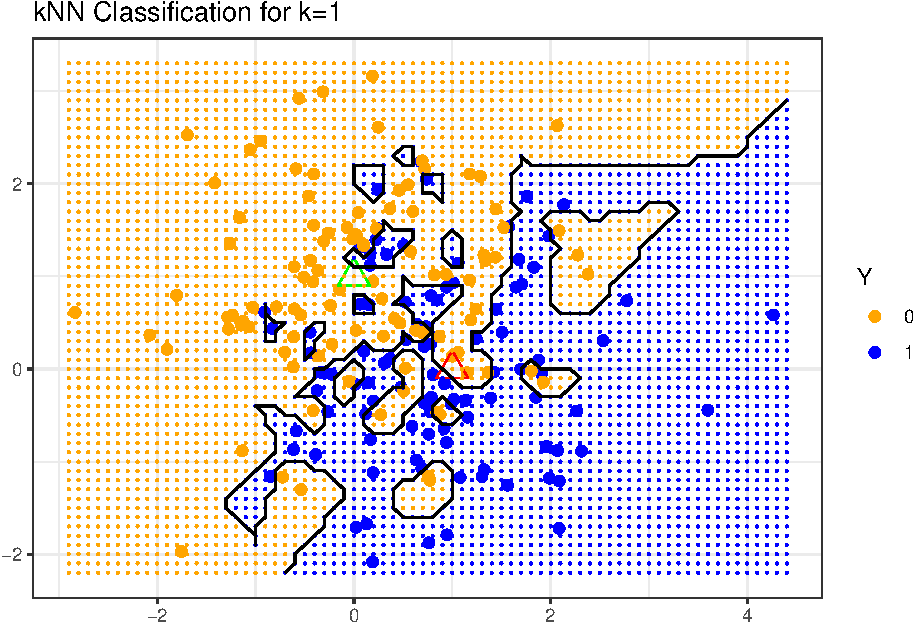
\includegraphics[keepaspectratio]{_main_files/figure-latex/unnamed-chunk-20-2.pdf}}

\subsubsection{Regression Classification}\label{regression-classification}

\begin{Shaded}
\begin{Highlighting}[]
\DocumentationTok{\#\# Grid Using Linear Model Classification}

\NormalTok{RegModel }\OtherTok{=} \FunctionTok{lm}\NormalTok{(}\FunctionTok{as.numeric}\NormalTok{(Ytrain)}\SpecialCharTok{{-}}\DecValTok{1} \SpecialCharTok{\textasciitilde{}}\NormalTok{ traindata)}
\NormalTok{beta.hat }\OtherTok{=} \FunctionTok{coef}\NormalTok{(RegModel)}

\DocumentationTok{\#\# We use the same ranges for the grid as before}

\NormalTok{Reg.yhat }\OtherTok{=} \FunctionTok{as.matrix}\NormalTok{(}\FunctionTok{cbind}\NormalTok{(}\FunctionTok{rep}\NormalTok{(}\DecValTok{1}\NormalTok{, }\FunctionTok{nrow}\NormalTok{(x.new)), x.new)) }\SpecialCharTok{\%*\%}\NormalTok{ beta.hat   }\DocumentationTok{\#\# predicted Y values}
\NormalTok{Reg.pred }\OtherTok{=} \FunctionTok{ifelse}\NormalTok{(Reg.yhat }\SpecialCharTok{\textgreater{}} \FloatTok{0.5}\NormalTok{, }\StringTok{"1"}\NormalTok{, }\StringTok{"0"}\NormalTok{)   }\DocumentationTok{\#\# convert numeric Y to factor}

\NormalTok{Reg.plot.data }\OtherTok{=} \FunctionTok{cbind}\NormalTok{(x.new, Reg.pred)}

\DocumentationTok{\#\# Basic plot is same as before, so now we add the regression boundary and classiffication results}
\NormalTok{reg.plot }\OtherTok{=}\NormalTok{ grid.plot }\SpecialCharTok{+} 
  \FunctionTok{theme\_bw}\NormalTok{() }\SpecialCharTok{+} 
  \FunctionTok{geom\_abline}\NormalTok{(}\AttributeTok{slope=}\SpecialCharTok{{-}}\NormalTok{beta.hat[}\DecValTok{2}\NormalTok{]}\SpecialCharTok{/}\NormalTok{beta.hat[}\DecValTok{3}\NormalTok{], }\AttributeTok{intercept=}\NormalTok{(.}\DecValTok{5}\SpecialCharTok{{-}}\NormalTok{beta.hat[}\DecValTok{1}\NormalTok{])}\SpecialCharTok{/}\NormalTok{beta.hat[}\DecValTok{3}\NormalTok{],}\AttributeTok{color=}\StringTok{"black"}\NormalTok{)  }\SpecialCharTok{+}
  \FunctionTok{geom\_point}\NormalTok{(}\AttributeTok{data =}\NormalTok{ Reg.plot.data, }\FunctionTok{aes}\NormalTok{(}\AttributeTok{x=}\NormalTok{X1, }\AttributeTok{y=}\NormalTok{X2, }\AttributeTok{color=}\NormalTok{Reg.pred), }\AttributeTok{size=}\FloatTok{0.05}\NormalTok{) }\SpecialCharTok{+}
  \FunctionTok{ggtitle}\NormalTok{(}\StringTok{"Regression Classification"}\NormalTok{)}

\FunctionTok{plot}\NormalTok{(reg.plot)}
\end{Highlighting}
\end{Shaded}

\pandocbounded{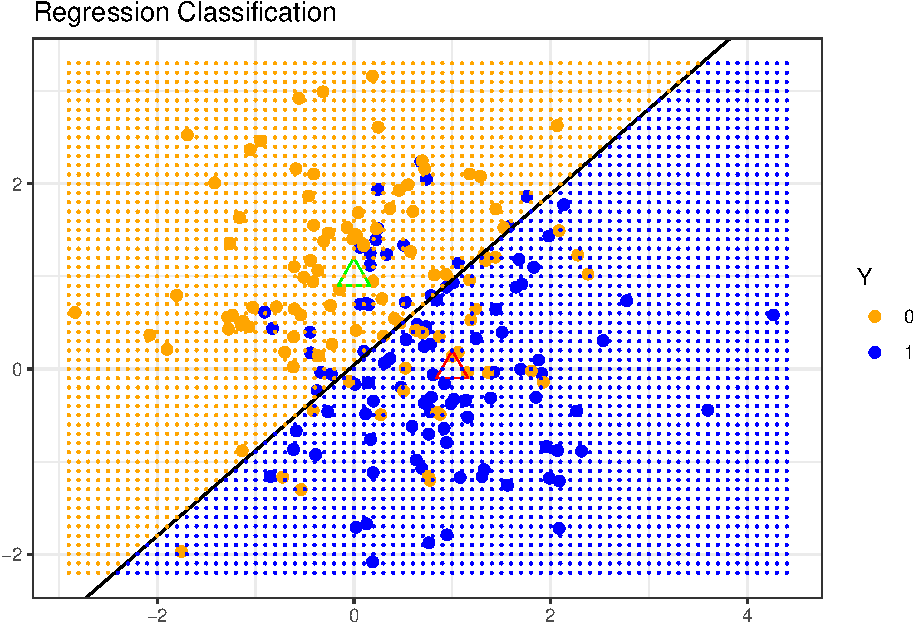
\includegraphics[keepaspectratio]{_main_files/figure-latex/unnamed-chunk-21-1.pdf}}

\subsubsection{Plot the Performance and Compare the two Methods}\label{plot-the-performance-and-compare-the-two-methods}

Test errors are in \texttt{magenta} and training errors are in \texttt{blue}. The upper \(x\)-coordinate indicates the \(k\) values, and the lower \(x\)-coordinate indicates the degrees-of-freedom of the \(k\)NN procedures so that the labels are reciprocally related to \(k\).

The training and test errors for linear regression are plotted at \(df = 3\) (corresponding to \(k = (2n)/3\)), since the linear model has 3 parameters, i.e., 3 dfs.

The training and test errors for KNN with \(k\) chosen by CV are plotted at the chose \(k\) values.

\begin{Shaded}
\begin{Highlighting}[]
\FunctionTok{plot}\NormalTok{(}\FunctionTok{c}\NormalTok{(}\FloatTok{0.5}\NormalTok{,m), }\FunctionTok{range}\NormalTok{(test.err.LS, train.err.LS, test.err.knn, train.err.knn),}
                  \AttributeTok{type=}\StringTok{"n"}\NormalTok{, }\AttributeTok{xlab=}\StringTok{"Degrees of Freedom"}\NormalTok{, }\AttributeTok{ylab=}\StringTok{"Error"}\NormalTok{, }\AttributeTok{xaxt=}\StringTok{"n"}\NormalTok{)}

\NormalTok{df }\OtherTok{=} \FunctionTok{round}\NormalTok{((}\DecValTok{2}\SpecialCharTok{*}\NormalTok{n)}\SpecialCharTok{/}\NormalTok{neighbor\_size)}
\FunctionTok{axis}\NormalTok{(}\DecValTok{1}\NormalTok{, }\AttributeTok{at=}\DecValTok{1}\SpecialCharTok{:}\NormalTok{m, }\AttributeTok{labels=}\NormalTok{df)}
\FunctionTok{axis}\NormalTok{(}\DecValTok{3}\NormalTok{, }\AttributeTok{at=}\DecValTok{1}\SpecialCharTok{:}\NormalTok{m, }\AttributeTok{labels=}\NormalTok{neighbor\_size)}

\FunctionTok{points}\NormalTok{(}\DecValTok{1}\SpecialCharTok{:}\NormalTok{m, test.err.knn, }\AttributeTok{col=}\StringTok{"magenta"}\NormalTok{, }\AttributeTok{pch=}\DecValTok{16}\NormalTok{)}
\FunctionTok{lines}\NormalTok{(}\DecValTok{1}\SpecialCharTok{:}\NormalTok{m, test.err.knn, }\AttributeTok{col=}\StringTok{"magenta"}\NormalTok{, }\AttributeTok{lty=}\DecValTok{1}\NormalTok{, }\AttributeTok{lwd=}\DecValTok{2}\NormalTok{)}
\FunctionTok{points}\NormalTok{(}\DecValTok{1}\SpecialCharTok{:}\NormalTok{m, train.err.knn, }\AttributeTok{col=}\StringTok{"blue"}\NormalTok{, }\AttributeTok{pch=}\DecValTok{16}\NormalTok{)}
\FunctionTok{lines}\NormalTok{(}\DecValTok{1}\SpecialCharTok{:}\NormalTok{m, train.err.knn, }\AttributeTok{col=}\StringTok{"blue"}\NormalTok{, }\AttributeTok{lty=}\DecValTok{3}\NormalTok{, }\AttributeTok{lwd=}\DecValTok{2}\NormalTok{)}

\FunctionTok{points}\NormalTok{(}\DecValTok{3}\NormalTok{, train.err.LS, }\AttributeTok{pch=}\DecValTok{2}\NormalTok{, }\AttributeTok{cex=}\DecValTok{2}\NormalTok{, }\AttributeTok{col=}\StringTok{"blue"}\NormalTok{)}
\FunctionTok{points}\NormalTok{(}\DecValTok{3}\NormalTok{, test.err.LS, }\AttributeTok{pch=}\DecValTok{2}\NormalTok{, }\AttributeTok{cex=}\DecValTok{2}\NormalTok{, }\AttributeTok{col=}\StringTok{"magenta"}\NormalTok{)}

\FunctionTok{points}\NormalTok{((}\DecValTok{1}\SpecialCharTok{:}\NormalTok{m)[neighbor\_size }\SpecialCharTok{==}\NormalTok{ k.optimal], train.err.knn.CV, }\AttributeTok{col=}\StringTok{"blue"}\NormalTok{, }\AttributeTok{pch=}\DecValTok{5}\NormalTok{, }\AttributeTok{cex=}\DecValTok{2}\NormalTok{)}
\FunctionTok{points}\NormalTok{((}\DecValTok{1}\SpecialCharTok{:}\NormalTok{m)[neighbor\_size }\SpecialCharTok{==}\NormalTok{ k.optimal], test.err.knn.CV, }\AttributeTok{col=}\StringTok{"magenta"}\NormalTok{, }\AttributeTok{pch=}\DecValTok{5}\NormalTok{, }\AttributeTok{cex=}\DecValTok{2}\NormalTok{)}

\FunctionTok{legend}\NormalTok{(}\StringTok{"bottomleft"}\NormalTok{, }\AttributeTok{pch =} \FunctionTok{c}\NormalTok{(}\DecValTok{2}\NormalTok{, }\DecValTok{2}\NormalTok{, }\DecValTok{5}\NormalTok{, }\DecValTok{5}\NormalTok{, }\DecValTok{16}\NormalTok{, }\DecValTok{16}\NormalTok{),  }\AttributeTok{col =} \FunctionTok{c}\NormalTok{(}\StringTok{"blue"}\NormalTok{, }\StringTok{"magenta"}\NormalTok{), }
       \AttributeTok{legend =} \FunctionTok{c}\NormalTok{(}\StringTok{"Regression Training Error"}\NormalTok{, }\StringTok{"Regression Testing Error"}\NormalTok{, }\StringTok{"kNN Optimal k Training Error"}\NormalTok{, }\StringTok{"kNN Optimal k Testing Error"}\NormalTok{, }\StringTok{"kNN different k Training Error"}\NormalTok{, }\StringTok{"kNN different k Testing Error"}\NormalTok{), }\AttributeTok{cex=}\FloatTok{0.75}\NormalTok{)}
\end{Highlighting}
\end{Shaded}

\pandocbounded{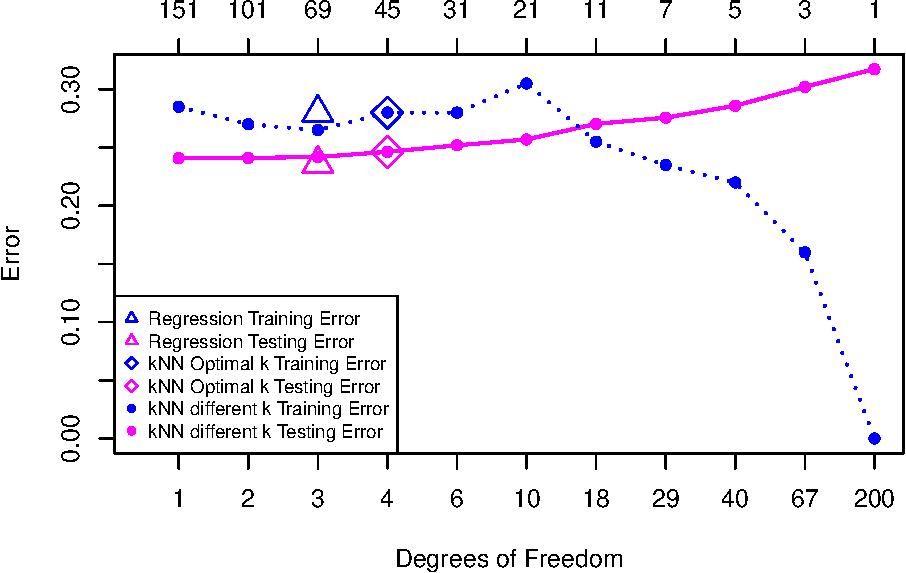
\includegraphics[keepaspectratio]{_main_files/figure-latex/unnamed-chunk-22-1.pdf}}

\chapter{Linear Regression Models}\label{linear-regression-models}

A regression model is a model for the \textbf{conditional expectation} of the response/ outcome variable given a set of predictors/features. A linear regression model specifically, is \emph{assumes} that \(E(Y|\mathbf{X}=\mathbf{x})\) is a linear function of the inputs \(X_1\), \(X_2\), \(\ldots\), \(X_p\), i.e.
\[E(Y|\mathbf{X}=\mathbf{x}) \sim \beta_0 + \beta_1 X_1 + \ldots + \beta_p X_p\]

To describe the properties and characteristics of the MLR model, we introduce the \texttt{Birthweight} example.

\textbf{Introduction to the \texttt{Birthweight} Example}

The goal of the birthweight study is to \textbf{predict} the birthweight (\emph{response}/ \emph{outcome}) of a newborn baby given a set of \emph{predictors}/\emph{features}, specifically for babies born prematurely.

The features include baby-related characteristics, such as length, weight, head circumference, gestation period, and parent characteristics, such as mother's/father's height, smoking habits, mother's pre-pregnancy weight, mother's/father's age, etc.

\begin{center}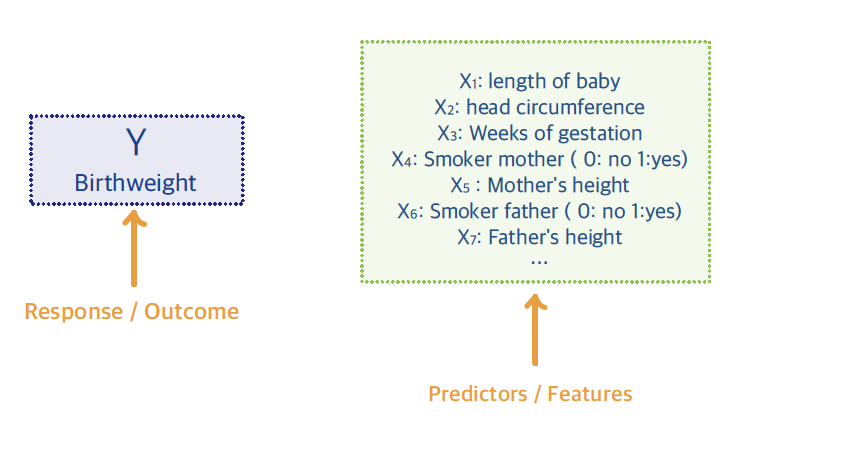
\includegraphics[width=0.7\linewidth]{images/week2/birthweight1a} \end{center}

The \textbf{predictors} we consider may be:

\begin{itemize}
\item
  \emph{quantitative}, such as length, weight, gestation period, etc.
\item
  \emph{qualitative/categorical}, such as smoking habits (yes/no), or
\item
  \emph{transformations of quantitative inputs}: For example, power transformation of variables, e.g.~\(X_3^3\); continuous functions of variables, e.g.~\(\log X_5\); basic expansions leading to a polynomial representation , e.g.~\(\sum_{k=1}^{n} c_k X_{7k}\); interactions, e.g.~\(X_1\cdot X_2\), etc.
\end{itemize}

\section{Multiple Linear Regression (MLR) Model}\label{multiple-linear-regression-mlr-model}

The model formulation is given by:

\textbf{Multiple Linear Regression Model}

\[ Y = \beta_0 + \beta_1 X_1 + \ldots + \beta_p X_p + \varepsilon \]
where

\begin{itemize}
\item
  \(\beta_0\) is the intercept
\item
  \(\beta_j\) is the regression coefficient associated with predictor \(X_j\)
\item
  \(\varepsilon\) is the error term
  Usual assumptions for the error terms are \(\varepsilon \sim IID \bigl(0, \sigma^2 \mathbf{I} \bigr)\)
\end{itemize}

Given the \textbf{training data} \(\bigl\{ x_{i1},\; x_{i2}, \ldots, x_{ip};\, y_i\bigr\}_{i=1}^{n}\), we can re-write the model as
\[ y_i = \beta_0 + \beta_1 x_{i1} + \ldots + \beta_p x_{ip} + \varepsilon_i,\,\, i=1, \ldots, n\]
where \(n\) is the sample size. Using the following matrix representation for the response and the features:
\[
    \mathbf{y}=\left(\begin{array}{c} 
      y_{1} \\ y_{2} \\ \vdots \\ y_{n}
    \end{array}\right)
    \quad
    \mathbf{\varepsilon}=\left(\begin{array}{c} 
      \varepsilon_{1} \\ \varepsilon_{2} \\ \vdots \\ \varepsilon_{n}
    \end{array}\right)
    \quad
    \mathbf{\beta}=\left(\begin{array}{c} 
      \beta_{0} \\ \beta_{1} \\ \vdots \\ \beta_p
    \end{array}\right)\quad
    \mathbf{X}=\left(\begin{array}{cccc}
    1 & x_{11} & \cdots & x_{1p} \\
    1 & x_{21} & \cdots & x_{2p}   \\
      \vdots & \vdots & \ddots & \vdots\\
   1 & x_{n1} & \cdots & x_{np}  \\
    \end{array} \right)
  \]
the model equation can be written in as
\[\left(\begin{array}{c} 
      y_{1} \\ y_{2} \\ \vdots \\ y_{n}
    \end{array}\right) = \left(\begin{array}{ccccc}
   1&x_{11}& \cdots &x_{1p} \\
   1& x_{21}& \cdots&x_{2p}   \\
   \vdots & \vdots & \ddots & \vdots\\
  1 & x_{n1} & \cdots & x_{np}  \\
    \end{array} \right) \left(\begin{array}{c} 
      \beta_{0} \\ \beta_{1} \\ \vdots \\ \beta_p
    \end{array}\right)\quad + 
\left(\begin{array}{c} 
      \varepsilon_{1} \\ \varepsilon_{2} \\ \vdots \\ \varepsilon_{n}
    \end{array}\right)
  \]
which leads to the concise form

\[
  \begin{array}{cccccc}
\mathbf{y}_{n\times 1} &=&\mathbf{X}_{n\times (p+1)}  &\mathbf{\beta}_{(p+1)\times 1}&+&\mathbf{\varepsilon}_{n\times 1}\\
\uparrow & & \uparrow & \uparrow & & \uparrow\\
\text{Response} &&\text{Design} & \text{Coefficients} & & \text{Error}\\
&&\text{Matrix} & && \text{Term}\\
\end{array}
\]
where \(n\) is the sample size, and \(p+1\) is number of predictors or columns of \(\mathbf{X}\) plus the intercept (the ``+1'').

\section{MLR Model Fitting}\label{mlr-model-fitting}

Given the training data \(\bigl\{ x_{i1},\; x_{i2}, \ldots, x_{ip};\, y_i\bigr\}_{i=1}^{n}\), we want to estimate \(\mathbf{\beta}\) , i.e.~express:
\[
    \hat{\mathbf{\beta}} \;=\; 
      \left(\hat{\beta}_0,\hat{\beta}_1,\ldots,\hat{\beta}_p\right)^{T}
  \]
as a \textbf{function of the data}.

The estimated regression coefficients \(\beta\) are obtained by minimizing the \emph{Residual Sum of Squares} (RSS):
\[RSS \;\;=\;\; ||\mathbf{y} - \mathbf{X} \beta||^2 = (\mathbf{y} - \mathbf{X} \beta)^{T} (\mathbf{y} - \mathbf{X}\beta)\]
The RSS minimizes the (Euclidean) distance of the points from the regression surface:

\begin{center}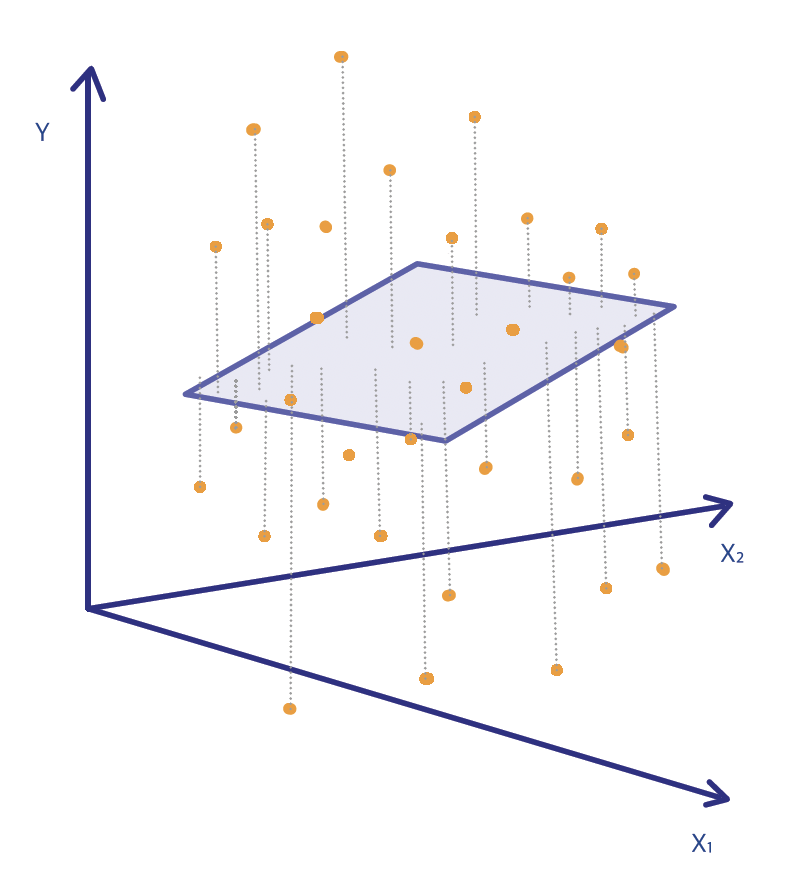
\includegraphics[width=0.4\linewidth]{images/week2/lsreg} \end{center}

This approach makes minimal assumptions, since it only requires that \((x_i, y_i)\) are \emph{random draws from their population}. Specifically, it makes \textbf{no assumptions} about the underlying distribution of the response. It simply finds the \textbf{best linear fit}, making no assumptions about model validity. In fact, the underlying (true) model does not even need to be linear for this approach to provide us with estimators. Therefore, it often gives good results, no matter how the data were obtained. If a linear model is a good approximation for the underlying non-linear (true) model, then the regression surface can also be thought as a criterion that measures the \textbf{lack-of-fit}.

\subsubsection*{Least-Squares Method}\label{least-squares-method-1}
\addcontentsline{toc}{subsubsection}{Least-Squares Method}

We want to estimate the \textbf{vector} of \(\mathbf{\beta}\) coefficients, by minimizing the \emph{sum of squared residuals}:
\[RSS\;\;=\;\; ||y - \mathbf{X} \beta||^2 = (y - \mathbf{X} \beta)^{T} (y - \mathbf{X}\beta)\]
Therefore, we take derivatives with respect to \(\beta\)'s and set to zero:
\begin{align*}
\frac{\partial RSS}{\partial \beta}  &= \mathbf{0}_{p\times 1} \,\, \Leftrightarrow \\
-2 \;\mathbf{X}^T_{p\times n} (y - \mathbf{X}\beta)_{n\times 1} &= \mathbf{0}_{p\times 1}
\end{align*}

This leads to the so-called \textbf{Normal Equations}
\[\mathbf{X}^T (y - \mathbf{X}\beta) = \mathbf{0}\]

Solving the Normal Equations
\[(\mathbf{X}^T\mathbf{X})\;\beta  = \mathbf{X}^T\; y  \]
leads to the

\textbf{Least Squares Estimators in MLR}
\[\hat{\beta} = (\mathbf{X}^T\mathbf{X})^{-1} \mathbf{X}^T\; y\]

We assume that \textbf{the rank of \(\mathbf{X}\) is \(p+1\)}, i.e.~no columns of \(\mathbf{X}\) are a linear combinations of the other columns of \(\mathbf{X}\). \emph{Since \(\mathbf{X}\) has rank \(p\), the inverse of \((\mathbf{X}^T\mathbf{X})\) exists}.

\subsubsection*{Fitted, Predicted Values \& Residuals}\label{fitted-predicted-values-residuals}
\addcontentsline{toc}{subsubsection}{Fitted, Predicted Values \& Residuals}

The \textbf{fitted value} of \(y_i\) at \(x_i = \bigl( x_{i1}, x_{i2}, \ldots , x_{ip}\bigr)\) is computed as:
\[\hat{y_{i}} = \hat{\beta}_0 + \hat{\beta}_1 x_{i1}+ \hat{\beta}_2 x_{i2} + \ldots + \hat{\beta}_p x_{ip}\]

More generally, using matrix formulation, we can compute the \textbf{fitted values} of \(\mathbf{y}\) based on the model as follows:
\begin{align*}
\hat{\mathbf{y}}_{n\times 1} &= \mathbf{X}  \hat{\beta} \\
&= \mathbf{X}  (\mathbf{X}^T\mathbf{X})^{-1} \mathbf{X}^T\; y\\
&=  \mathbf{X}  (\mathbf{X}^T\mathbf{X})^{-1} \mathbf{X}^T\; y := \mathbf{H}_{n \times n} y_{n\times 1}
\end{align*}

\textbf{The Hat Matrix}

We define
\[ \mathbf{H}_{n \times n} =  \mathbf{X}  (\mathbf{X}^T\mathbf{X})^{-1} \mathbf{X}^T\]
to be the \textbf{hat matrix}, since it returns the ``\emph{y-hat}'' values.

The \textbf{predicted} value of \(y_i\) at \(x_i^* = \bigl( x_{i1}^*, x_{i2}^*, \ldots , x_{ip}^*\bigr)\) is given by
\[\hat{\mathbf{y}}^* = \hat{\beta}_0 + \hat{\beta}_1 x_{i1}^* + \hat{\beta}_2 x_{i2}^* + \ldots + \hat{\beta}_p x_{ip}^*\]
More generally, using matrix formulation, the \textbf{predicted values} of \(\mathbf{y}\) are given by
\[\hat{\mathbf{y}}^* = \mathbf{X}^* \hat{\beta}\]

\begin{quote}
Note that the difference between the fitted and predicted values is that the \(\mathbf{x}\) is a vector of features that we have already observed (it is part of our training data), while \(\mathbf{x}^*\) is an \textbf{unobserved} vector of features that is \textbf{independent} of the training data.
\end{quote}

The \textbf{residual} of \(y_i\) at \(x_i = \bigl( x_{i1}, x_{i2}, \ldots , x_{ip}\bigr)\) is obtained by
\begin{align*}
r_{i} &= y_i - \hat{y}_i \\
&= y_i - \hat{\beta}_0 - \hat{\beta}_1 x_{i1} - \hat{\beta}_2 x_{i2} - \ldots - \hat{\beta}_p x_{ip}
\end{align*}

Using matrix formulation, the residuals can be computed as
\begin{align*}
\mathbf{r}_{n\times 1} &= \mathbf{y} - \hat{\mathbf{y}} \\
&= \mathbf{y} - \mathbf{X}\hat{\beta} = \mathbf{y} - \mathbf{X} (\mathbf{X}^T\mathbf{X})^{-1} \mathbf{X}^T\;  y \\
&= \mathbf{y} - \mathbf{H} \mathbf{y} = (\mathbf{I} -\mathbf{H}) \mathbf{y}
\end{align*}

The residuals \(\mathbf{r}\) are used to estimate the \textbf{error variance}:
\[\hat{\sigma}^2 = \frac{1}{n-p-1}\sum_i r_i^2 = \frac{RSS}{n-p-1}\]
Note that the denominator in the formula is equal to the \emph{degrees of freedom of the residuals} \((n-p-1)\).

\subsubsection*{Properties of the Residuals}\label{properties-of-the-residuals}
\addcontentsline{toc}{subsubsection}{Properties of the Residuals}

The LS estimator is the \(\beta\) vector that satisfies the \textbf{normal equations}, that is
\[\mathbf{X}^T (\mathbf{y} - \hat{\mathbf{y}}) = \mathbf{X}^T (\mathbf{y} - \mathbf{X}\hat{\beta}) = \mathbf{0}\]

Based on this, we can derive the following properties for the residuals \(\mathbf{r}_{n\times 1}\):

\begin{itemize}
\item
  The cross-products between the residual vector \(\mathbf{r}\) and \emph{each column of \(\mathbf{X}\)} are zero, i.e.~
  \begin{align*}
  \mathbf{X}^T\; \mathbf{r} &= \mathbf{X}^T (\mathbf{y}-\mathbf{X}\hat{\beta})\\
  &= \mathbf{X}^T \mathbf{y} - \mathbf{X}^T\mathbf{X}\hat{\beta}\\
  &= \mathbf{X}^T \mathbf{y} -  (\mathbf{X}^T \mathbf{X} )(\mathbf{X}^T\mathbf{X})^{-1} \mathbf{X}^T\; \mathbf{y} = \mathbf{0}
  \end{align*}
\item
  The cross-product between the fitted value \(\hat{y}\) and the residual vector \(r\) is zero, i.e.
  \[\hat{\mathbf{y}}^T \;\mathbf{r} = \hat{\beta}^{T} \mathbf{X}^{T} \;\mathbf{r} = \mathbf{0}\]
  This implies that the residual vector \(\mathbf{r}\) is \textbf{orthogonal to each column of \(\mathbf{X}\) and to \(\hat{\mathbf{y}}\)}.
\end{itemize}

\section{Least-Squares \& Normal Equations}\label{least-squares-normal-equations}

In this section, we focus on the system of linear equations that we solve to obtain the least squares estimators for \(\beta\). Recall, that we want to find a a vector \(\hat{\beta}\) that minimizes:
\[\min_{\beta} ||\mathbf{y} - \mathbf{X} \beta||^2\]
\emph{Any vector that provides a minimum value for this expression is called a least-squares solution}.

The set of all least squares solutions is precisely the \textbf{set of solutions} to
\[(\mathbf{X}^T \mathbf{X}) \beta = \mathbf{X}^T \mathbf{y}\]
There is a \emph{unique} solution \textbf{if and only if} \(rank(\mathbf{X}) = p+1\) in which case \(\bigl(\mathbf{X}^T \mathbf{X}\bigr)\) is invertible.

\subsection*{System of Linear Equations}\label{system-of-linear-equations}

\paragraph*{Linear Algebra Review}\label{linear-algebra-review}
\addcontentsline{toc}{paragraph}{Linear Algebra Review}

Let us review a few facts from linear algebra related to solutions to a system of linear equations. For simplicity in the notation, we use the \emph{generic} system of equations:
\[\mathbf{A} z = c\]
where
\[ \mathbf{A}=\left(\begin{array}{cccc}
    a_{11} & a_{12} & \cdots & a_{1k} \\
    a_{21} & a_{22} & \cdots & a_{2k}   \\
      \vdots & \vdots & \ddots & \vdots\\
  a_{m1} & a_{m2} & \cdots & a_{mk}  \\
    \end{array} \right),\quad
    z =\left(\begin{array}{c}
    z_{1} \\
    z_{2}   \\
   \vdots\\
    z_{m}  \\
    \end{array} \right),\quad
    c =\left(\begin{array}{c}
    c_{1} \\
    c_{2}   \\
   \vdots\\
    c_{m}  \\
    \end{array} \right)
    \]

Denote by \(\mathbf{A}_{i} = \bigl( a_{1i}, a_{2i}, \ldots, a_{mi}\bigr)^T\) the vector representing the \emph{columns} of \(\mathbf{A}\). Therefore, \(\mathcal{C}(\mathbf{A})\) is the space generated by the columns of \(\mathbf{A}\), or in other words the \(span \bigl(\mathbf{A}_1, \mathbf{A}_2, \ldots, \mathbf{A}_{k}\bigr)\).

\textbf{Definition}

The \textbf{span} of a collection of vectors \(\bigl(\mathbf{A}_1, \mathbf{A}_2, \ldots, \mathbf{A}_{k}\bigr)\) is the set of all linear combinations of these vectors:
\begin{align*}
&span \bigl(\mathbf{A}_1, \mathbf{A}_2, \ldots, \mathbf{A}_{k}\bigr) \\
&= \Bigl\{ d_1 \mathbf{A}_1 + d_2 \mathbf{A}_2 + \ldots + d_k \mathbf{A}_{k}, \text{ for any constants } d_1, \ldots, d_k \in \mathbb{R}
\Bigr\}
\end{align*}

The column space of \(\mathbf{A}\), \(\mathcal{C}(\mathbf{A})\), is a \textbf{subspace} in \(\mathbb{R}^n\). A linear subspace of \(\mathbb{R}^n\) is thought of as a ``flat'' surface within \(\mathbb{R}^n\), and it is a collection of vectors that is closed under linear combinations. Illustration of subspaces of \(\mathbb{R}^n\) are shown below:

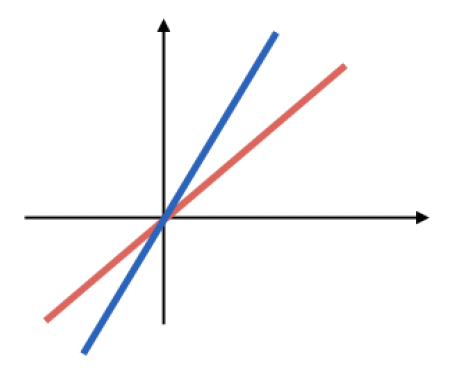
\includegraphics[width=0.35\linewidth,height=\textheight,keepaspectratio]{images/week2/subspace1.png} 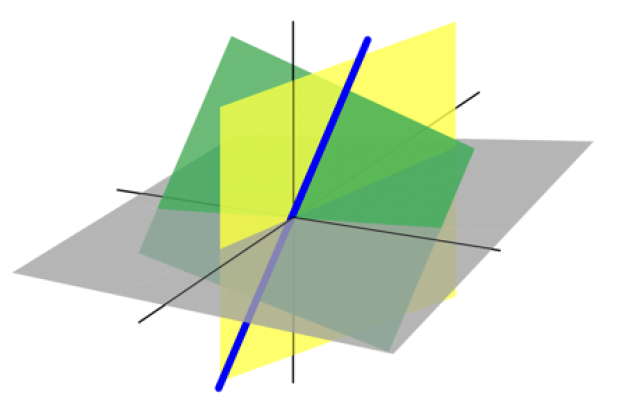
\includegraphics[width=0.35\linewidth,height=\textheight,keepaspectratio]{images/week2/subspace2.png}

\subsubsection*{\texorpdfstring{Solving the System of Equations \(\mathbf{A}z=c\)}{Solving the System of Equations \textbackslash mathbf\{A\}z=c}}\label{solving-the-system-of-equations-mathbfazc}
\addcontentsline{toc}{subsubsection}{Solving the System of Equations \(\mathbf{A}z=c\)}

For a system of equations, \(\mathbf{A} z = c\), to have a solution, \(c\) must be a linear combination of the columns of \(\mathbf{A}\), i.e.~\(c \in \mathcal{C}(\mathbf{A})\). This is simply obtained by the definition of \emph{matrix multiplication} and \emph{equality}:
\[\mathbf{A} z = c \, \Leftrightarrow \, c = z_1 \mathbf{A}_1 + \ldots + z_k \mathbf{A}_k\]

When \(c \notin \mathcal{C}(\mathbf{A})\), we need to \textbf{find \(\hat{c}\) living in \(\mathcal{C}(\mathbf{A})\) that is closest to \(c\)}. If this is the case, \(\mathbf{A} z = \hat{c}\) has a unique solution, and \(\hat{c}\) comes as close to the original data as possible.
To do so, we need to \textbf{project} \(c\) \textbf{orthogonally} onto \(\mathcal{C}(\mathbf{A})\), by multiplying both sides by \(\mathbf{A}^T\):

\[\mathbf{A}^T\mathbf{A} z = \mathbf{A}^T c\]
* These are the normal equations.

In the sketch to the right, \(\mathcal{C}(\mathbf{A})\), the space spanned by the columns of \(\mathbf{A}\), is a \emph{flat} surface, and \(c\) is a point that exists off of that flat surface. The \textbf{shortest distance} from the point \(c\) to the plane \(\mathcal{C}(\mathbf{A})\) is the one \emph{orthogonal} to the plane.

The \emph{normal equations} essentially help us find the closest point to \(c\) that belongs \(\mathcal{C}\bigl(\mathbf{A}\Bigr)\) by means of an orthogonal projection.

\subsection*{Geometric Representation of LS}\label{geometric-representation-of-ls}

Taking the previous discussion to the linear regression framework:

\begin{itemize}
\item
  \(\mathcal{C}(\mathbf{X})\) is the space that is \emph{spanned} by the predictors \(X_1\), \(X_2\), \(\ldots\), \(X_p\), or in other words the columns of the design matrix. It is a \emph{flat} subspace of \(\mathbb{R}^n\).
\item
  The response \(\mathbf{y}\) is a vector \textbf{off} the subspace, and the fitted value \(\hat{\mathbf{y}}\) is the orthogonal projection of \(\mathbf{y}\) onto \(\mathcal{C}(\mathbf{X})\).
\item
  The residuals, on the other hand, \(\mathbf{r} = \mathbf{y} - \hat{\mathbf{y}}\) are \textbf{orthogonal} to \(\hat{\mathbf{y}}\) and to \(\mathcal{C}\bigl( \mathbf{X} \bigr)\).
\end{itemize}

Essentially, what the least-squares method does is that it decomposes the data vector \(\mathbf{y}\) into two orthogonal components:
\[\mathbf{y}_{n\times 1} = \hat{\mathbf{y}}_{n\times 1} + \mathbf{r}_{n\times 1}\]

\section{\texorpdfstring{Goodness-Of-Fit: \(R\)-Square}{Goodness-Of-Fit: R-Square}}\label{goodness-of-fit-r-square}

A measure of how well the model fits the data is the \textbf{\(R\)-square} or the so-called \textbf{coefficient of determination} or \emph{percentage of variance explained}. It is defined as

\begin{align*}
R^2 &=  \frac{\sum_i (\hat{y}_i - \bar{y})^2}{\sum_i (y_i - \bar{y})^2}\quad = \frac{\text{distance of model from grand mean}}{\text{distance of observations from grand mean }}\\ 
& =  \frac{||\hat{\mathbf{y}} - \bar{\mathbf{y}}||^2}{||\mathbf{y} - \bar{\mathbf{y}}||^2} \\
&= \frac{||\mathbf{y} - \bar{\mathbf{y}}||^2 - ||\hat{\mathbf{y}} - \mathbf{y}||^2  }{||\mathbf{y} - \bar{\mathbf{y}}||^2} \\
&= 1 - \frac{||\hat{\mathbf{y}} - \mathbf{y}||^2 }{||\mathbf{y} - \bar{\mathbf{y}}||^2}\, := 1 - \frac{RSS}{TSS}
\end{align*}
where we used orthogonality to get\\
\[\underbrace{||\mathbf{y} - \bar{\mathbf{y}}||^2}_{\substack{\text{ total}\\\text{ variation  }}} = \underbrace{||\hat{\mathbf{y}} - \bar{\mathbf{y}}||^2}_{\substack{\text{ model variation }\\ \text{ from mean }}} + \underbrace{|| \hat{\mathbf{y}} - \mathbf{y}||^2}_{\text{ error  }}\]

\paragraph*{\texorpdfstring{Properties of \(R^2\) }{Properties of R\^{}2 }}\label{properties-of-r2}
\addcontentsline{toc}{paragraph}{Properties of \(R^2\) }

\begin{itemize}
\item
  \(0\leq R^2 \leq 1\)
\item
  \(R^2\) is invariant of any location and/or scale change of \(Y\) or \(X\).
\item
  \(R^2\) alone does not tell us much about the effectiveness of the LS method.
\item
  A small \(R^2\) does not imply that the LS model is bad.
\item
  Adding a new predictor, even if it is randomly generated and has nothing to do with \(Y\) will decrease \(RSS\) and therefore increase \(R^2\). These relationships are illustrated in the two plots below:
\end{itemize}

\begin{center}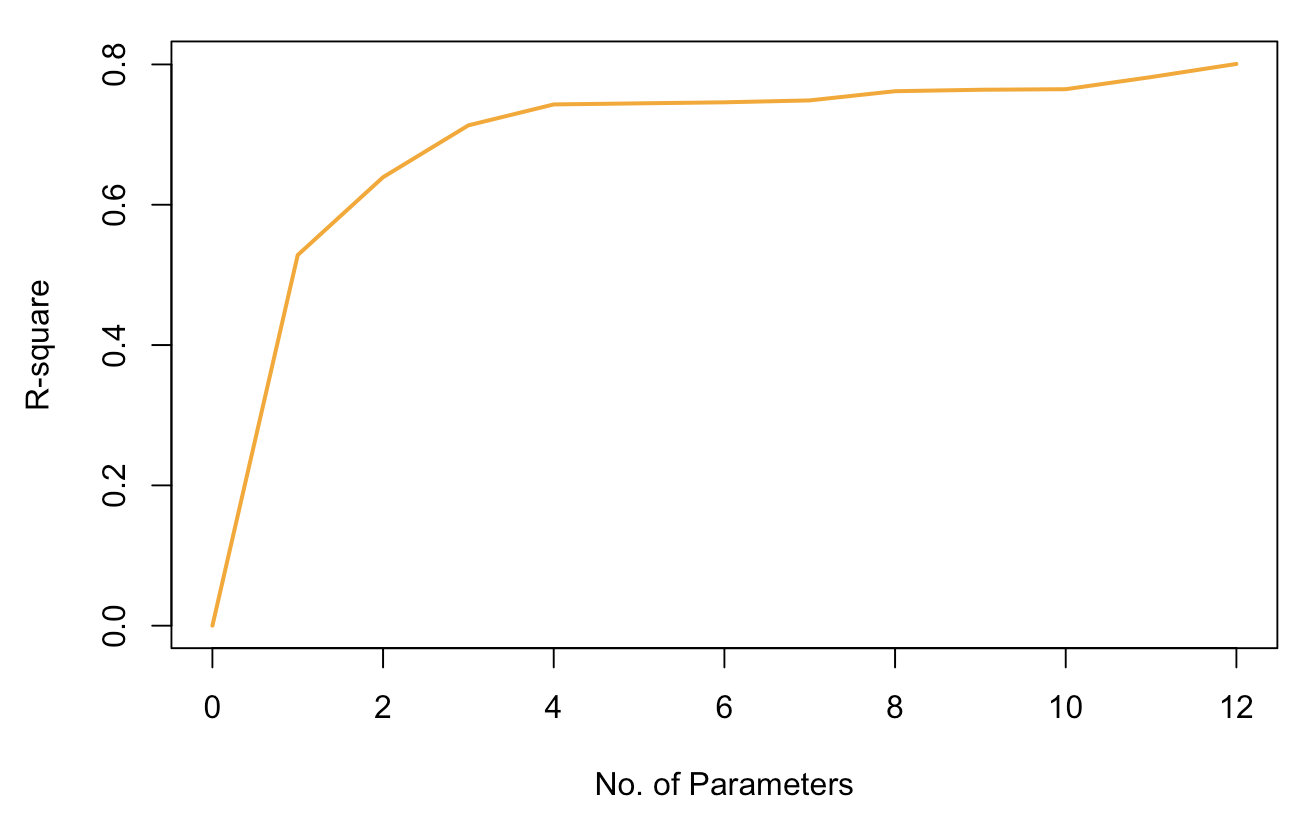
\includegraphics[width=0.6\linewidth]{images/week2/rsq} \end{center}

\begin{center}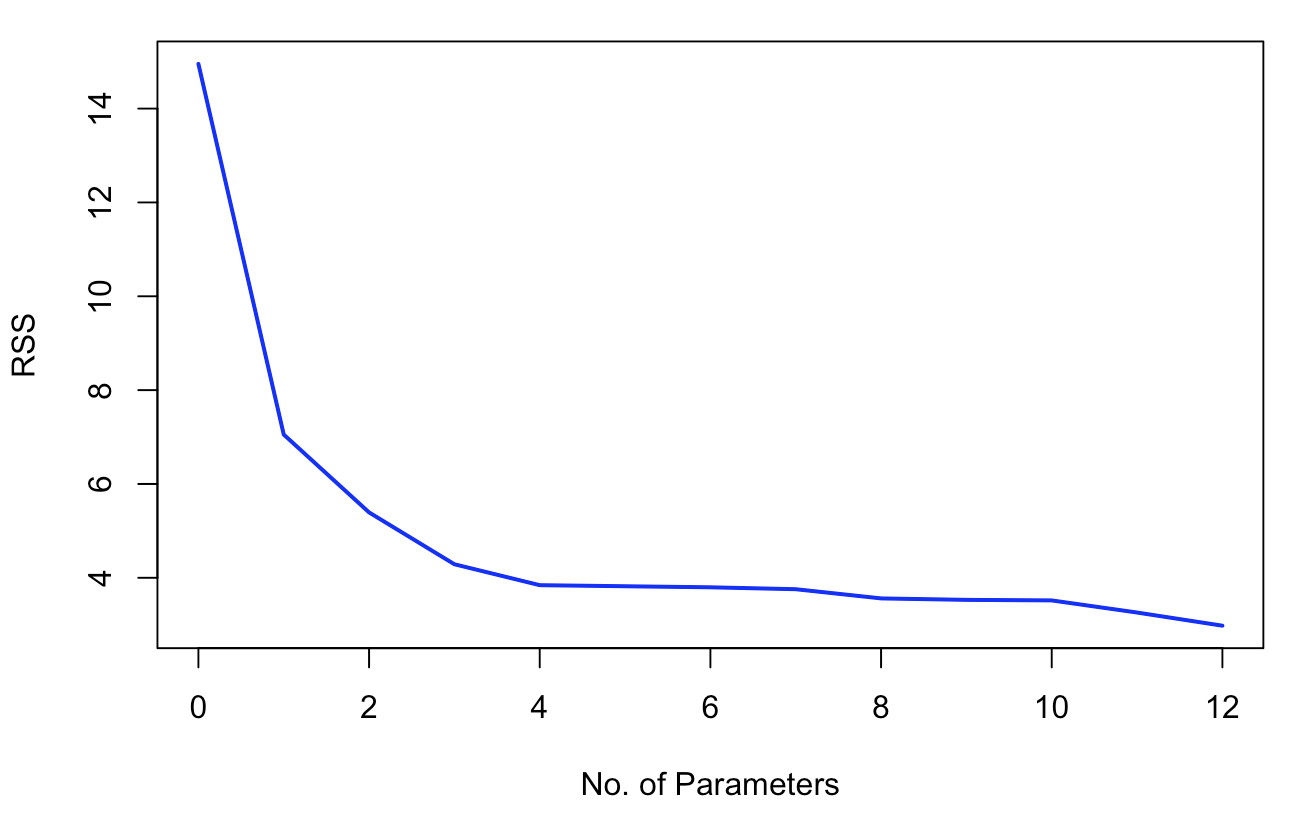
\includegraphics[width=0.6\linewidth]{images/week2/rss} \end{center}

\section{\texorpdfstring{Linear Transformations on \(X\)}{Linear Transformations on X}}\label{linear-transformations-on-x}

Suppose we have a linear regression model of \(Y\) on \(X\). If we \textbf{scale} or \textbf{shift} a predictor, then
the fitted values, \(\hat{\mathbf{y}}\), and \(R^2\) stay the same, but LS estimators, \(\hat{\beta}\), change!

\paragraph*{Some Examples}\label{some-examples}
\addcontentsline{toc}{paragraph}{Some Examples}

\begin{itemize}
\item
  As an example, consider scaling a predictor, i.e.~\(\tilde{x}_{i2} =  2 x_{i2}\) or \(\tilde{x}_{i3} =  x_{i3}/4\). This transformation will not impact \(\hat{\mathbf{y}}\), or \(R^2\).
\item
  In the \texttt{birthweight} example, the length of a baby is given in cm. If we want to change the unit to inches by dividing by 2.54 the column that corresponds to length, i.e.~\(\tilde{X}_1 = X_1/2.54\), then this won't affect our predicted values.
\end{itemize}

These statements hold true, if we apply any linear transformation on the \(p\) predictors \textbf{as long as the transformation does not change the rank of \(\mathbf{X}\)}.

\section{Rank deficiency}\label{rank-deficiency}

The design matrix \(\mathbf{X}\) is an \(n\times p\) matrix. If this matrix is \textbf{not of full rank} (i.e., its columns are not linearly independent), the matrix \(\mathbf{X}^T \mathbf{X}\) can not be inverted. This implies that there is some redundancy in the columns of \(\mathbf{X}\), i.e.~one column can be written as a linear combination of other columns. As a result, the matrix \(\mathbf{X^T X}\) is \emph{singular} which means that the LS solution is not unique (\emph{identifiability problem}).

However, \(\mathcal{C}(\mathbf{X})\) is well defined and thus \(\hat{y}\) is well-defined and can be computed. \texttt{R}/ \texttt{Python} can cope well with this problem, and the returned model can be used for prediction.

\section{Hypothesis Testing in MLR}\label{hypothesis-testing-in-mlr}

When fitting a regression model, we often want to understand which predictors are statistically significant or which model (a larger or a smaller) is more appropriate --either for prediction or for estimation purposes--.

Testing for the statistical significance of one (or more) predictor(s), can be formulated as testing whether the corresponding \(\beta\) is zero, or as a model comparison test.In this class, we summarize all testing questions as the following hypothesis test:

\[
\begin{cases}
& H_0: \text{ Reduced Model with } p_0 \text{ coefficients}\\
& H_{\alpha}: \text{ Full/ Larger Model with } p_{\alpha} \text{ coefficients}\\
\end{cases}
\]
Obviously, \(p_{\alpha} > p_0\), since the reduced model is a subset/special case of the full model. Therefore, we expect the reduced model to have \(RSS_0\) smaller than \(RSS_{\alpha}\), the full model's \(RSS\), since \(p_{\alpha} > p_0\). In this context, the main tool for testing is the so-called \textbf{partial \(F\) test} and is formulated as follows:

\textbf{Partial \(F\) test}

\emph{Hypothesis Test:}
\[
\begin{cases}
& H_0: \text{ Reduced Model with } p_0 \text{ coefficients}\\
& H_{\alpha}: \text{ Full/ Larger Model with } p_{\alpha} \text{ coefficients}\\
\end{cases}
\]

\emph{Test Statistic:}
\[F=\frac{\bigl(RSS_0 - RSS_{\alpha}\bigr)/p_{\alpha} - p_0}{RSS_{\alpha}/ \bigl(n-p_{\alpha} \bigr)}\,  \sim \, F_{p_{\alpha} - p_0, n-p_{\alpha}}\]

\emph{Decision Rule:}
Reject \(H_0\), if the \(F\) test statistic is large (or larger than \(F_{p_{\alpha} - p_0, n-p_{\alpha}}\)), i.e.~the variation missed by the reduced model, when being compared with the error variance, is significantly large.

\begin{itemize}
\item
  The \textbf{numerator} in the partial \(F\) test quantifies the variation in the data not explained by the reduced model, but explained by the full model.
\item
  On the other hand, the \textbf{denomimator} is equal to the variation in the data not explained by the full model (i.e., not explained by either model), which is used to estimate the error variance.
\end{itemize}

\textbf{Birthweight Example (cont'd)}

We want to decide whether the group of the predictors that refer to father's characteristics (i.e.~variables \(X_9\) -- \(X_{12}\)) are significant --as a group.

The hypothesis test is formulated as
\[\begin{cases}
 &H_0: Y \sim  1+  \beta_{1} X_{1} + \ldots + \beta_{8}X_{8} \\
 & H_{\alpha}:  Y \sim  1+  \beta_1 X_1 + \ldots + \beta_{8}X_{8}+ \ldots + \beta_{12} X_{12} 
 \end{cases} 
 \]
In this case \(p_0 = 8+1\) is the number of \(\beta\)'s in the reduced model, and \(p_{\alpha}=12+1\) is the number of \(\beta\)'s in the full model. Using \texttt{R}/\texttt{Python}, we extract \(RSS_0\), \(RSS_{\alpha}\) to perform the partial \(F\) test and make a decision.

It turns out that \(F = 0.7225\) is smaller than \(F_{p_{\alpha} - p_0, n-p_{\alpha}}=2.7\) meaning that the model under the null (reduced) is preferred.

\subsubsection*{\texorpdfstring{Partial \(F\) Test: Special Cases }{Partial F Test: Special Cases }}\label{partial-f-test-special-cases}
\addcontentsline{toc}{subsubsection}{Partial \(F\) Test: Special Cases }

\begin{itemize}
\tightlist
\item
  \textbf{Test for a Single Predictor \(\beta_j\)}
\end{itemize}

\[\begin{cases}
 & H_0: Y \sim  1+  \beta_1 X_1 + \ldots + \beta_{j-1}X_{j-1} + \qquad \quad \; \beta_{j+1} X_{j+1} + \ldots + \beta_p X_p \\
 & H_{\alpha}:  Y \sim  1+  \beta_1 X_1 + \ldots + \beta_{j-1}X_{j-1} +  \beta_{j} X_{j} + \beta_{j+1} X_{j+1} + \ldots + \beta_p X_p \\
 \end{cases} 
 \]
is equivalent to the so-called \textbf{\(t\)-test for each regression parameter}.

\begin{itemize}
\tightlist
\item
  \textbf{Test for all Predictors}
\end{itemize}

\[\begin{cases}
 &H_0: Y \sim  1 \qquad \text{[intercept-only model]} \\
 & H_{\alpha}:  Y \sim  1+  \beta_1 X_1 + \ldots + \beta_{j-1}X_{j-1} +  \beta_{j} X_{j} + \beta_{j+1} X_{j+1} + \ldots + \beta_p X_p \\
 \end{cases} 
 \]
This is the \textbf{overall \(F\)} test that can be thought of as a \emph{goodness-of-fit test}.

\section{Categorical Variables in MLR}\label{categorical-variables-in-mlr}

As we discussed some of the predictors may be \emph{categorical}. Assume a predictor that is categorical with \(k\) levels. When added in a linear regression model, it is coded as \emph{\(k-1\) numerical predictors}. The default coding is of the form:
\[D_i=\left\{\begin{array}{cl}
            0, & \mbox{if not level $i$} \\
            1, & \mbox{if level $i$}
        \end{array}\right .\]
where Level \(1\) is the \emph{reference level}.

\textbf{An Example with Categorical Variables}

Consider a categorical predictor with three levels (\(a\), \(b\), \(c\)):

\[\left(\begin{array}{c} 
      a \\ a \\ b \\ b \\ b \\ c \\ c
    \end{array}\right)
    \Longrightarrow 
    \left(\begin{array}{ccc} 
      1 & 0 & 0\\ 1 & 0 & 0\\ 0 & 1 & 0\\ 0 & 1 & 0 \\ 0 & 1 & 0\\ 0 & 0 & 0\\ 0& 0 & 0
    \end{array}\right)
    \]

In this setup,

\begin{itemize}
\item
  Col 1 corresponds to level \(a\), i.e.~\(X_1 = 1\) if in column 1, and \(0\) otherwise.
\item
  Col 2 corresponds to level \(b\), i.e.~\(X_2 = 1\) if in column 2, and \(0\) otherwise.
\item
  Col 3 corresponds to level \(c\): this is the reference level, since its value is absorbed by the intercept.
\end{itemize}

\begin{quote}
In general, any level can be chosen to be the reference level; this is more a choice that depends on the context rather than the statistics behind. There are also alternative ways to code the variables. If we choose a different coding, then this will affect the estimated regression coefficients (and the interpretation), but it won't affect the predicted/fitted values.
\end{quote}

\section{Collinearity}\label{collinearity}

In practice, we often encounter problems in which many of the predictors are \textbf{highly correlated} with each other. In such cases, the fitted values and sampling variance of the regression coefficients can be highly dependent on the particular predictors chosen for the model. This results in sensitive and unreliable estimators.

Possible \emph{symptoms} of collinearity include :

\begin{enumerate}
\def\labelenumi{(\roman{enumi})}
\item
  high pair-wise (sample) correlation between predictors,
\item
  relatively large \(R^2\),
\item
  statistically significant \(F\) test without \emph{any} statistically significant predictors.
\end{enumerate}

There are also specific tests and metrics that allow us to assess the severity of collinearity in our model, but this is beyond the scope of this course.

The easiest way to \textbf{remedy} collinearity is to remove some predictors from highly correlated groups of predictors. Other (more advanced) approaches include PCA, or regularization using penalized Least Squares.

\section{Model Diagnostics}\label{model-diagnostics}

We made several assumptions when defining the linear regression model:
\[\mathbf{y} =  \mathbf{X}\beta + \varepsilon,\,\, \text{ where } \,\, \varepsilon \sim IID(0, \sigma^2)\]

This means that we assumed:

\begin{itemize}
\item
  \emph{Linearity}, i.e.~the model is linear with respect to the predictors.
\item
  \emph{Constant Variance}, i.e.~all \(Y\)'s have common, constant variance.
\item
  \emph{Uncorrelated errors}, i.e.~\(Y_i\) and \(Y_j\) are uncorrelated for \(i\neq j\).
\item
  \emph{(Normality)}: this is not part of the assumptions above, and it is not required for the derivation of the least-squares estimators. However, it is needed when one wants to discuss statistical properties of the estimators and the fitted values and residuals. It is, in particular, one of the most critical assumptions when it comes to hypothesis testing.
\end{itemize}

If we are interested in using the model for understanding the effect of the predictors on the response (i.e.~not purely for prediction purposes), then we need to make sure that all assumptions are satisfied (via diagnostic test/plots), and if not take appropriate actions (remedial measures).

Since the focus of this class is prediction, we refer the students to a regression course or textbook to review diagnostics and remedial measures for a MLR model. As an example, you can refer to \ldots{}

\subsection*{Outliers}\label{outliers}

Finally, outliers might be a concern both in large and smaller data sets. If the data set is not very large, it is suggested to test for outliers, e.g.~using outlier tests based on the leave-one-out prediction error. Otherwise, if the data set is really large, then this test is not useful and it is suggested to adjust for multiple comparisons or consider alternative approaches.

If outliers seem to be an issue, then it is important to (i) know the range of each variable, (ii) apply log, square-root or other transformations on right skewed predictors and \(Y\), or (iii) apply winsorization to remove the effect of extreme values.

\section{\texorpdfstring{The \texttt{Birthweight} Data Set Example}{The Birthweight Data Set Example}}\label{the-birthweight-data-set-example}

The \texttt{birthweight.csv} data set contains data from a study on the birth weight of \textbf{42} babies. The variables in the data set are the following:

\begin{itemize}
\tightlist
\item
  \texttt{ID}: Unique Identification number of a baby
\item
  \texttt{Length}: Length of the baby at time of birth in cm (\(X_1\))
\item
  \texttt{Birthweight}: Weight of the baby at time of birth in kg (\(Y\))
\item
  \texttt{Headcirc}: Head circumference of the baby at time of birth in cm (\(X_2\))
\item
  \texttt{Gestation}: Completed weeks of gestation (\(X_3\))
\item
  \texttt{smoker}: Mother is/is not a smoker \{0: No, 1: Yes\} (\(X_4\))
\item
  \texttt{mage}: Mother's age at time of birth (\(X_5\))
\item
  \texttt{mnocig}: Mother's number of cigarettes smoked per day (\(X_6\))
\item
  \texttt{mheight}: Mother's height in cm (\(X_7\))
\item
  \texttt{mppwt}: Mother's pre-pregnancy weight (\(X_8\))
\item
  \texttt{fage}: Father's age at time of birth (\(X_9\))
\item
  \texttt{fedyrs}: Father's years of education (\(X_{10}\))
\item
  \texttt{fnocig}: Father's number of cigarettes smoked per day (\(X_{11}\))
\item
  \texttt{fheight}: Father's height (\(X_{12}\))
\end{itemize}

\begin{Shaded}
\begin{Highlighting}[]
\NormalTok{birthweight }\OtherTok{\textless{}{-}} \FunctionTok{read.csv}\NormalTok{(}\StringTok{"data/week2/Birthweight.csv"}\NormalTok{, }\AttributeTok{header=}\ConstantTok{TRUE}\NormalTok{)}
\FunctionTok{dim}\NormalTok{(birthweight)}
\end{Highlighting}
\end{Shaded}

\begin{verbatim}
## [1] 42 14
\end{verbatim}

\begin{Shaded}
\begin{Highlighting}[]
\FunctionTok{head}\NormalTok{(birthweight)}
\end{Highlighting}
\end{Shaded}

\begin{verbatim}
##     ID Length Birthweight Headcirc Gestation smoker mage mnocig mheight mppwt
## 1 1360     56        4.55       34        44      0   20      0     162    57
## 2 1016     53        4.32       36        40      0   19      0     171    62
## 3  462     58        4.10       39        41      0   35      0     172    58
## 4 1187     53        4.07       38        44      0   20      0     174    68
## 5  553     54        3.94       37        42      0   24      0     175    66
## 6 1636     51        3.93       38        38      0   29      0     165    61
##   fage fedyrs fnocig fheight
## 1   23     10     35     179
## 2   19     12      0     183
## 3   31     16     25     185
## 4   26     14     25     189
## 5   30     12      0     184
## 6   31     16      0     180
\end{verbatim}

Since the \texttt{ID} variable is not of interest in our analysis, we won't use it in our analysis. For convenience can remove it from the data frame we are working with:

\begin{Shaded}
\begin{Highlighting}[]
\NormalTok{birthweight }\OtherTok{=}\NormalTok{ birthweight[,}\SpecialCharTok{{-}}\DecValTok{1}\NormalTok{]}
\end{Highlighting}
\end{Shaded}

\subsubsection{Fitting a Multiple Linear Regression}\label{fitting-a-multiple-linear-regression}

We start by fitting a linear regression model using all the predictors and we print the summary of the LS results:

\begin{Shaded}
\begin{Highlighting}[]
\NormalTok{birthweight.mlr.full }\OtherTok{=} \FunctionTok{lm}\NormalTok{(Birthweight}\SpecialCharTok{\textasciitilde{}}\NormalTok{., }\AttributeTok{data=}\NormalTok{birthweight)}
\FunctionTok{summary}\NormalTok{(birthweight.mlr.full)}
\end{Highlighting}
\end{Shaded}

\begin{verbatim}
## 
## Call:
## lm(formula = Birthweight ~ ., data = birthweight)
## 
## Residuals:
##      Min       1Q   Median       3Q      Max 
## -0.37925 -0.25558 -0.05541  0.21700  0.60329 
## 
## Coefficients:
##              Estimate Std. Error t value Pr(>|t|)   
## (Intercept) -3.812311   2.080150  -1.833  0.07713 . 
## Length       0.034152   0.031456   1.086  0.28656   
## Headcirc     0.086594   0.029489   2.937  0.00644 **
## Gestation    0.096565   0.031323   3.083  0.00447 **
## smoker      -0.243895   0.168516  -1.447  0.15854   
## mage        -0.019004   0.018537  -1.025  0.31374   
## mnocig       0.001064   0.006854   0.155  0.87770   
## mheight      0.004187   0.014153   0.296  0.76944   
## mppwt        0.010346   0.011228   0.921  0.36443   
## fage         0.007187   0.016327   0.440  0.66305   
## fedyrs       0.003220   0.030939   0.104  0.91783   
## fnocig       0.003445   0.004013   0.858  0.39769   
## fheight     -0.013293   0.009614  -1.383  0.17731   
## ---
## Signif. codes:  0 '***' 0.001 '**' 0.01 '*' 0.05 '.' 0.1 ' ' 1
## 
## Residual standard error: 0.3342 on 29 degrees of freedom
## Multiple R-squared:  0.7834, Adjusted R-squared:  0.6938 
## F-statistic: 8.742 on 12 and 29 DF,  p-value: 1.011e-06
\end{verbatim}

If we want to check the objects returned by \texttt{lm} and \texttt{summary(lm...)}:

\begin{Shaded}
\begin{Highlighting}[]
\FunctionTok{names}\NormalTok{(birthweight.mlr.full)}
\end{Highlighting}
\end{Shaded}

\begin{verbatim}
##  [1] "coefficients"  "residuals"     "effects"       "rank"         
##  [5] "fitted.values" "assign"        "qr"            "df.residual"  
##  [9] "xlevels"       "call"          "terms"         "model"
\end{verbatim}

\begin{Shaded}
\begin{Highlighting}[]
\FunctionTok{names}\NormalTok{(}\FunctionTok{summary}\NormalTok{(birthweight.mlr.full)) }
\end{Highlighting}
\end{Shaded}

\begin{verbatim}
##  [1] "call"          "terms"         "residuals"     "coefficients" 
##  [5] "aliased"       "sigma"         "df"            "r.squared"    
##  [9] "adj.r.squared" "fstatistic"    "cov.unscaled"
\end{verbatim}

The design matrix in this example can be extracted using:

\begin{Shaded}
\begin{Highlighting}[]
\NormalTok{design.birthweight }\OtherTok{=} \FunctionTok{model.matrix}\NormalTok{(birthweight.mlr.full);}
\end{Highlighting}
\end{Shaded}

If we want to extract the Regression coefficients including the intercept, i.e.~\(\hat{\beta}\), we have

\begin{Shaded}
\begin{Highlighting}[]
\NormalTok{birthweight.mlr.full}\SpecialCharTok{$}\NormalTok{coef}
\end{Highlighting}
\end{Shaded}

\begin{verbatim}
##  (Intercept)       Length     Headcirc    Gestation       smoker         mage 
## -3.812311183  0.034151922  0.086594329  0.096565435 -0.243895136 -0.019003806 
##       mnocig      mheight        mppwt         fage       fedyrs       fnocig 
##  0.001064074  0.004187315  0.010346096  0.007187428  0.003219952  0.003444674 
##      fheight 
## -0.013293205
\end{verbatim}

The fitted values and residuals are obtained by:

\begin{Shaded}
\begin{Highlighting}[]
\NormalTok{full.model.residuals }\OtherTok{=}\NormalTok{ birthweight.mlr.full}\SpecialCharTok{$}\NormalTok{resid}
\NormalTok{full.model.fitted }\OtherTok{=}\NormalTok{ birthweight.mlr.full}\SpecialCharTok{$}\NormalTok{fitted}
\end{Highlighting}
\end{Shaded}

Check the calculation for Residual standard error and Multiple R-squared in the summary output:

The residuals \(\mathbf{r}\) are used to estimate the \textit{error variance}:
\[\hat{\sigma}^2 = \frac{1}{n-p-1}\sum_i r_i^2 = \frac{RSS}{n-p-1}\]
To obtain and estimator for \(\hat{\sigma}\), we can either use the formula (from the notes):

\begin{Shaded}
\begin{Highlighting}[]
\NormalTok{n }\OtherTok{=} \FunctionTok{dim}\NormalTok{(birthweight)[}\DecValTok{1}\NormalTok{]}
\NormalTok{p }\OtherTok{=} \FunctionTok{dim}\NormalTok{(birthweight)[}\DecValTok{2}\NormalTok{] }\SpecialCharTok{{-}} \DecValTok{1}
\FunctionTok{sqrt}\NormalTok{(}\FunctionTok{sum}\NormalTok{(birthweight.mlr.full}\SpecialCharTok{$}\NormalTok{residuals}\SpecialCharTok{\^{}}\DecValTok{2}\NormalTok{)}\SpecialCharTok{/}\NormalTok{(n}\SpecialCharTok{{-}}\NormalTok{ p }\SpecialCharTok{{-}} \DecValTok{1}\NormalTok{))}
\end{Highlighting}
\end{Shaded}

\begin{verbatim}
## [1] 0.3341631
\end{verbatim}

or we can extract it from the \texttt{lm} object:

\begin{Shaded}
\begin{Highlighting}[]
\FunctionTok{summary}\NormalTok{(birthweight.mlr.full)}\SpecialCharTok{$}\NormalTok{sigma}
\end{Highlighting}
\end{Shaded}

\begin{verbatim}
## [1] 0.3341631
\end{verbatim}

The coefficient of determination computes as:
\[ \frac{\sum_i (\hat{y}_i - \bar{y})^2}{\sum_i (y_i - \bar{y})^2} = 1 - \frac{RSS}{TSS}\]
We can extract \(R^2\) from the summary output or compute it:

\begin{Shaded}
\begin{Highlighting}[]
\FunctionTok{summary}\NormalTok{(birthweight.mlr.full)}\SpecialCharTok{$}\NormalTok{r.squared}
\end{Highlighting}
\end{Shaded}

\begin{verbatim}
## [1] 0.783425
\end{verbatim}

\begin{Shaded}
\begin{Highlighting}[]
\DecValTok{1} \SpecialCharTok{{-}} \FunctionTok{sum}\NormalTok{(birthweight.mlr.full}\SpecialCharTok{$}\NormalTok{residuals}\SpecialCharTok{\^{}}\DecValTok{2}\NormalTok{)}\SpecialCharTok{/}\NormalTok{(}\FunctionTok{var}\NormalTok{(birthweight}\SpecialCharTok{$}\NormalTok{Birthweight)}\SpecialCharTok{*}\NormalTok{(n}\DecValTok{{-}1}\NormalTok{))}
\end{Highlighting}
\end{Shaded}

\begin{verbatim}
## [1] 0.783425
\end{verbatim}

\begin{Shaded}
\begin{Highlighting}[]
\DecValTok{1} \SpecialCharTok{{-}} \FunctionTok{var}\NormalTok{(birthweight.mlr.full}\SpecialCharTok{$}\NormalTok{residuals)}\SpecialCharTok{/}\FunctionTok{var}\NormalTok{(birthweight}\SpecialCharTok{$}\NormalTok{Birthweight)}
\end{Highlighting}
\end{Shaded}

\begin{verbatim}
## [1] 0.783425
\end{verbatim}

\subsubsection{\texorpdfstring{Invariance of \(R^2\) \& Fitted Values}{Invariance of R\^{}2 \& Fitted Values}}\label{invariance-of-r2-fitted-values}

We can also check the invariance property of \(R^2\) by rescaling one of the variables:

\begin{Shaded}
\begin{Highlighting}[]
\DocumentationTok{\#\# Center the Length variable}
\NormalTok{birthweight.new }\OtherTok{=}\NormalTok{ birthweight}
\NormalTok{birthweight.new}\SpecialCharTok{$}\NormalTok{Length.new }\OtherTok{=}\NormalTok{ birthweight.new}\SpecialCharTok{$}\NormalTok{Length }\SpecialCharTok{{-}} \FunctionTok{rep}\NormalTok{(}\FunctionTok{mean}\NormalTok{(birthweight.new}\SpecialCharTok{$}\NormalTok{Length), }\DecValTok{42}\NormalTok{)}

\DocumentationTok{\#\# Model with original \textasciigrave{}Length\textasciigrave{}}
\FunctionTok{summary}\NormalTok{(}\FunctionTok{lm}\NormalTok{(Birthweight}\SpecialCharTok{\textasciitilde{}}\NormalTok{., }\AttributeTok{data=}\NormalTok{birthweight.new[}\SpecialCharTok{{-}}\DecValTok{14}\NormalTok{]))}\SpecialCharTok{$}\NormalTok{r.squared}
\end{Highlighting}
\end{Shaded}

\begin{verbatim}
## [1] 0.783425
\end{verbatim}

\begin{Shaded}
\begin{Highlighting}[]
\DocumentationTok{\#\# Model with centered \textasciigrave{}Length\textasciigrave{}}
\FunctionTok{summary}\NormalTok{(}\FunctionTok{lm}\NormalTok{(Birthweight}\SpecialCharTok{\textasciitilde{}}\NormalTok{., }\AttributeTok{data=}\NormalTok{birthweight.new[}\SpecialCharTok{{-}}\DecValTok{1}\NormalTok{]))}\SpecialCharTok{$}\NormalTok{r.squared}
\end{Highlighting}
\end{Shaded}

\begin{verbatim}
## [1] 0.783425
\end{verbatim}

If we want, we can also check that the fitted values from both models are identical:

\begin{Shaded}
\begin{Highlighting}[]
\DocumentationTok{\#\# Difference in fitted values between Model w \textasciigrave{}Length\textasciigrave{} {-}  Model w \textasciigrave{}centered{-}Length\textasciigrave{}}
\DocumentationTok{\#\#\# The values are added to make the output cleaner.}

\FunctionTok{sum}\NormalTok{( }\FunctionTok{fitted}\NormalTok{(}\FunctionTok{lm}\NormalTok{(Birthweight}\SpecialCharTok{\textasciitilde{}}\NormalTok{., }\AttributeTok{data=}\NormalTok{birthweight.new[}\SpecialCharTok{{-}}\DecValTok{14}\NormalTok{])) }\SpecialCharTok{{-}} \FunctionTok{fitted}\NormalTok{(}\FunctionTok{lm}\NormalTok{(Birthweight}\SpecialCharTok{\textasciitilde{}}\NormalTok{., }\AttributeTok{data=}\NormalTok{birthweight.new[}\SpecialCharTok{{-}}\DecValTok{1}\NormalTok{])) )}
\end{Highlighting}
\end{Shaded}

\begin{verbatim}
## [1] -8.881784e-16
\end{verbatim}

Note that the difference is not exactly 0, since there are rounding errors that accumulated when the various R functions are applied.

\subsubsection{\texorpdfstring{\(R^2\) and \(RSS\) behavior when adding more \(X\)s}{R\^{}2 and RSS behavior when adding more Xs}}\label{r2-and-rss-behavior-when-adding-more-xs}

We can also visualize how the \(R^2\) and \(RSS\) change as a function of the number of variables in the model to observe that adding a new predictor, even if it is randomly generated and has nothing to do with \(Y\) will decrease \(RSS\) and therefore increase \(R^2\).

So, start with the null model that contains only the intercept and then we add variables one at a time, keeping the \(R^2\) and \(RSS\) that we will plot in the end. We will also randomly generate a new variable \texttt{randomvar} to illustrate that even an unrelevant variable has an effect on both \(R^2\) and \(RSS\):

\begin{Shaded}
\begin{Highlighting}[]
\NormalTok{birthweight.new }\OtherTok{=}\NormalTok{ birthweight}
\NormalTok{birthweight.new}\SpecialCharTok{$}\NormalTok{randomvar }\OtherTok{=} \FunctionTok{rnorm}\NormalTok{(}\DecValTok{42}\NormalTok{)}
\end{Highlighting}
\end{Shaded}

\begin{Shaded}
\begin{Highlighting}[]
\NormalTok{no.var }\OtherTok{=} \DecValTok{0}\SpecialCharTok{:}\DecValTok{12}
\FunctionTok{par}\NormalTok{(}\AttributeTok{mfrow=}\FunctionTok{c}\NormalTok{(}\DecValTok{1}\NormalTok{,}\DecValTok{2}\NormalTok{))}
\FunctionTok{plot}\NormalTok{(no.var, rsq, }\AttributeTok{xlab=}\StringTok{"No. of Parameters"}\NormalTok{, }\AttributeTok{ylab =} \StringTok{"R{-}square"}\NormalTok{, }\AttributeTok{type=}\StringTok{\textquotesingle{}n\textquotesingle{}}\NormalTok{);}
\FunctionTok{lines}\NormalTok{(no.var, rsq, }\AttributeTok{lwd=}\DecValTok{2}\NormalTok{, }\AttributeTok{col=}\StringTok{"orange"}\NormalTok{)}
\FunctionTok{plot}\NormalTok{(no.var, rss, }\AttributeTok{xlab=}\StringTok{"No. of Parameters"}\NormalTok{, }\AttributeTok{ylab =} \StringTok{"RSS"}\NormalTok{, }\AttributeTok{type=}\StringTok{\textquotesingle{}n\textquotesingle{}}\NormalTok{);}
\FunctionTok{lines}\NormalTok{(no.var, rss, }\AttributeTok{lwd=}\DecValTok{2}\NormalTok{, }\AttributeTok{col=}\StringTok{"blue"}\NormalTok{)}
\end{Highlighting}
\end{Shaded}

\pandocbounded{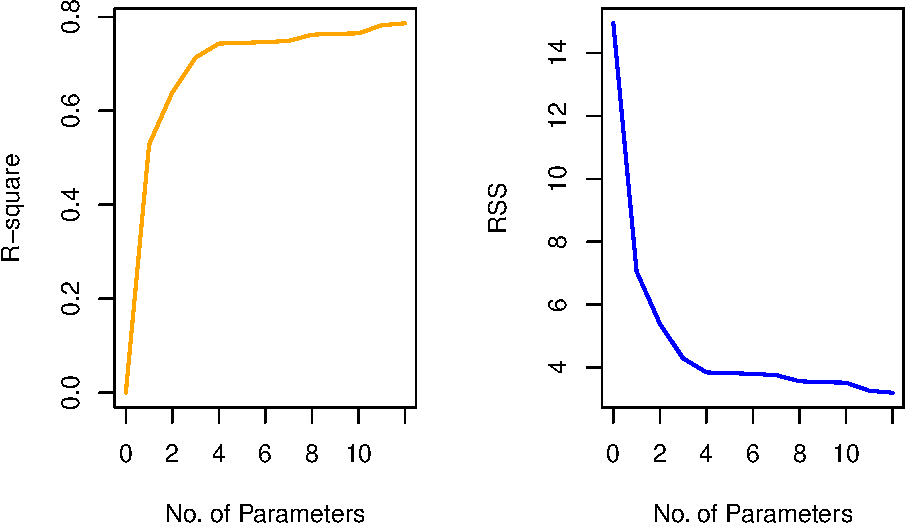
\includegraphics[keepaspectratio]{_main_files/figure-latex/unnamed-chunk-41-1.pdf}}

This is to illustrate why \(R^2\) and \(RSS\) are not good metrics when it comes to model selection. They are useful, because they helps us understand the quality of the model or \(RSS\) is a key ingredient in constructing hypothesis tests, but they are never used for model selection.

\subsubsection{Rank Deficiency}\label{rank-deficiency-1}

We have rank deficiency when \(\mathbf{X}\) is not of full rank which leads to the \((\mathbf{X}^T\mathbf{X})\) matrix not being invertible.

Here we illustrate a scenario where it is easy to identify the cause of the problem.

\begin{Shaded}
\begin{Highlighting}[]
\DocumentationTok{\#\# Create a new variable: the average height of both parents}
\NormalTok{birthweight.new }\OtherTok{=}\NormalTok{ birthweight}
\NormalTok{birthweight.new}\SpecialCharTok{$}\NormalTok{aveheight }\OtherTok{=}\NormalTok{ (birthweight.new}\SpecialCharTok{$}\NormalTok{mheight}\SpecialCharTok{+}\NormalTok{birthweight.new}\SpecialCharTok{$}\NormalTok{fheight)}\SpecialCharTok{/}\DecValTok{2}

\DocumentationTok{\#\# Regress birthweight against all predictors}
\FunctionTok{summary}\NormalTok{(}\FunctionTok{lm}\NormalTok{(Birthweight }\SpecialCharTok{\textasciitilde{}}\NormalTok{ ., }\AttributeTok{data=}\NormalTok{birthweight.new))}
\end{Highlighting}
\end{Shaded}

\begin{verbatim}
## 
## Call:
## lm(formula = Birthweight ~ ., data = birthweight.new)
## 
## Residuals:
##      Min       1Q   Median       3Q      Max 
## -0.37925 -0.25558 -0.05541  0.21700  0.60329 
## 
## Coefficients: (1 not defined because of singularities)
##              Estimate Std. Error t value Pr(>|t|)   
## (Intercept) -3.812311   2.080150  -1.833  0.07713 . 
## Length       0.034152   0.031456   1.086  0.28656   
## Headcirc     0.086594   0.029489   2.937  0.00644 **
## Gestation    0.096565   0.031323   3.083  0.00447 **
## smoker      -0.243895   0.168516  -1.447  0.15854   
## mage        -0.019004   0.018537  -1.025  0.31374   
## mnocig       0.001064   0.006854   0.155  0.87770   
## mheight      0.004187   0.014153   0.296  0.76944   
## mppwt        0.010346   0.011228   0.921  0.36443   
## fage         0.007187   0.016327   0.440  0.66305   
## fedyrs       0.003220   0.030939   0.104  0.91783   
## fnocig       0.003445   0.004013   0.858  0.39769   
## fheight     -0.013293   0.009614  -1.383  0.17731   
## aveheight          NA         NA      NA       NA   
## ---
## Signif. codes:  0 '***' 0.001 '**' 0.01 '*' 0.05 '.' 0.1 ' ' 1
## 
## Residual standard error: 0.3342 on 29 degrees of freedom
## Multiple R-squared:  0.7834, Adjusted R-squared:  0.6938 
## F-statistic: 8.742 on 12 and 29 DF,  p-value: 1.011e-06
\end{verbatim}

As you see the \(\beta_j\) that corresponds to the new variable cannot be calculated (hence the \texttt{NA}), since \texttt{aveheight} is linearly dependent on both \texttt{mheight} and \texttt{fheight}. At the same time, although the matrix \(\mathbf{X}\) is not of full rank, \texttt{R} produces solutions for the rest of the \(\beta\)s and the fitted model is valid for prediction purposes. The predictions derived from this model will align with those obtained from fitting a linear regression model excluding the columns with NA coefficient.

This issue can be easily fixed, by removing one or more variables. Which variable will be removed depends on the context. For example, we need to (conceptually) answer the question on whether we prefer to have the \texttt{aveheight} or each parent's height individually.

A harder issue to resolve is when two predictors are not exaclty linearly dependent, but approximately - this means that they are highly correlated, but not an exact function of one another. This is more challenging to deal with and we will discuss it later.

\subsubsection{Test for the Significance of Predictors}\label{test-for-the-significance-of-predictors}

We use the partial \(F\) test
\[F=\frac{\bigl(RSS_0 - RSS_{\alpha}\bigr)/p_{\alpha} - p_0}{RSS_{\alpha}/ \bigl(n-p_{\alpha} \bigr)}\,  \sim \, F_{p_{\alpha} - p_0, n-p_{\alpha}}\]
to compare the full model with all available predictors versus the model that exclude father-related variables. That is, the hypothesis test is formulated as
\[\begin{cases}
 &H_0: Y \sim  1+  \beta_{1} X_{1} + \ldots + \beta_{8}X_{8} \\
 & H_{\alpha}:  Y \sim  1+  \beta_1 X_1 + \ldots + \beta_{8}X_{8}+ \ldots + \beta_{12} X_{12} 
 \end{cases} 
 \]

\begin{Shaded}
\begin{Highlighting}[]
\DocumentationTok{\#\# Full Model was fitted before }
\DocumentationTok{\#\# and is stored in birthweight.mlr.full}

\DocumentationTok{\#\# Reduced Model }
\NormalTok{birthweight.mlr.reduced1 }\OtherTok{=} \FunctionTok{lm}\NormalTok{(Birthweight}\SpecialCharTok{\textasciitilde{}}\NormalTok{ Length}\SpecialCharTok{+}\NormalTok{Headcirc}\SpecialCharTok{+}\NormalTok{Gestation}\SpecialCharTok{+}\NormalTok{smoker}\SpecialCharTok{+}\NormalTok{mage}\SpecialCharTok{+}\NormalTok{mnocig}\SpecialCharTok{+}\NormalTok{mheight}\SpecialCharTok{+}\NormalTok{mppwt,  }\AttributeTok{data=}\NormalTok{birthweight)}
\end{Highlighting}
\end{Shaded}

We can use one function to perform the test:

\begin{Shaded}
\begin{Highlighting}[]
\FunctionTok{anova}\NormalTok{(birthweight.mlr.reduced1, birthweight.mlr.full)}
\end{Highlighting}
\end{Shaded}

\begin{verbatim}
## Analysis of Variance Table
## 
## Model 1: Birthweight ~ Length + Headcirc + Gestation + smoker + mage + 
##     mnocig + mheight + mppwt
## Model 2: Birthweight ~ Length + Headcirc + Gestation + smoker + mage + 
##     mnocig + mheight + mppwt + fage + fedyrs + fnocig + fheight
##   Res.Df    RSS Df Sum of Sq      F Pr(>F)
## 1     33 3.5610                           
## 2     29 3.2383  4   0.32271 0.7225 0.5837
\end{verbatim}

The \(F\) statistic value is 0.7225, and the corresponding \(p\)-value is 0.5837 which means that we fail to reject the null and conclude that the model under the \(H_0\) is preferred. In other words, we prefer the smaller model which implies that the father-related predictors can be removed from the model.

We can also build the \(F\) statistic, by extracting all necessary components:

\begin{Shaded}
\begin{Highlighting}[]
\NormalTok{RSS0 }\OtherTok{=} \FunctionTok{deviance}\NormalTok{(birthweight.mlr.reduced1)}
\NormalTok{RSS0}
\end{Highlighting}
\end{Shaded}

\begin{verbatim}
## [1] 3.560996
\end{verbatim}

\begin{Shaded}
\begin{Highlighting}[]
\NormalTok{RSSalpha }\OtherTok{=} \FunctionTok{deviance}\NormalTok{(birthweight.mlr.full)}
\NormalTok{RSSalpha}
\end{Highlighting}
\end{Shaded}

\begin{verbatim}
## [1] 3.238285
\end{verbatim}

\begin{Shaded}
\begin{Highlighting}[]
\NormalTok{p0 }\OtherTok{=}\DecValTok{9}\NormalTok{;}
\NormalTok{palpha }\OtherTok{=} \DecValTok{13}\NormalTok{;}
\NormalTok{n}\OtherTok{=}\DecValTok{42}\NormalTok{;}

\DocumentationTok{\#\# Partial F test}
\NormalTok{F }\OtherTok{=}\NormalTok{ ((RSS0 }\SpecialCharTok{{-}}\NormalTok{ RSSalpha)}\SpecialCharTok{/}\NormalTok{(palpha}\SpecialCharTok{{-}}\NormalTok{p0))}\SpecialCharTok{/}\NormalTok{(RSSalpha}\SpecialCharTok{/}\NormalTok{(n}\SpecialCharTok{{-}}\NormalTok{palpha))}
\NormalTok{F}
\end{Highlighting}
\end{Shaded}

\begin{verbatim}
## [1] 0.7224983
\end{verbatim}

\begin{Shaded}
\begin{Highlighting}[]
\DocumentationTok{\#\# Critical value use to compare with the F statistic.}
\FunctionTok{qf}\NormalTok{(}\FloatTok{0.95}\NormalTok{, palpha}\SpecialCharTok{{-}}\NormalTok{p0, n}\SpecialCharTok{{-}}\NormalTok{palpha)}
\end{Highlighting}
\end{Shaded}

\begin{verbatim}
## [1] 2.701399
\end{verbatim}

the conclusion is the same since \(F < F_{p_{\alpha}-p_0, n-p_{\alpha}}\).

\subsubsection{\texorpdfstring{Testing for a Single \(\beta_j\)}{Testing for a Single \textbackslash beta\_j}}\label{testing-for-a-single-beta_j}

Let's test for the significance of variable \texttt{Length} (\(X_1\)), i.e.
\[\begin{cases}
 &H_0: Y \sim  1 + \qquad \quad  \beta_2 X_2 + \ldots + \beta_{12}X_{12} \\
 & H_{\alpha}:  Y \sim  1+  \beta_1 X_1+  \beta_2 X_2 + \ldots + \beta_{12} X_{12} \\
 \end{cases} 
 \]

We fit the full model and then compare by means of the partial \(F\) test:

\begin{Shaded}
\begin{Highlighting}[]
\DocumentationTok{\#\# Full Model was fitted before }
\DocumentationTok{\#\# and is stored in birthweight.mlr.full}

\DocumentationTok{\#\# Reduced Model }
\NormalTok{birthweight.mlr.reduced2 }\OtherTok{=} \FunctionTok{lm}\NormalTok{(Birthweight}\SpecialCharTok{\textasciitilde{}}\NormalTok{ Headcirc}\SpecialCharTok{+}\NormalTok{Gestation}\SpecialCharTok{+}\NormalTok{smoker}\SpecialCharTok{+}\NormalTok{mage}\SpecialCharTok{+}\NormalTok{mnocig}\SpecialCharTok{+}\NormalTok{mheight}\SpecialCharTok{+}\NormalTok{mppwt}\SpecialCharTok{+}\NormalTok{fage}\SpecialCharTok{+}\NormalTok{fedyrs}\SpecialCharTok{+}\NormalTok{fnocig}\SpecialCharTok{+}\NormalTok{fheight,  }\AttributeTok{data=}\NormalTok{birthweight)}

\DocumentationTok{\#\# Partial $F$ test}
\FunctionTok{anova}\NormalTok{(birthweight.mlr.reduced2, birthweight.mlr.full)}
\end{Highlighting}
\end{Shaded}

\begin{verbatim}
## Analysis of Variance Table
## 
## Model 1: Birthweight ~ Headcirc + Gestation + smoker + mage + mnocig + 
##     mheight + mppwt + fage + fedyrs + fnocig + fheight
## Model 2: Birthweight ~ Length + Headcirc + Gestation + smoker + mage + 
##     mnocig + mheight + mppwt + fage + fedyrs + fnocig + fheight
##   Res.Df    RSS Df Sum of Sq      F Pr(>F)
## 1     30 3.3699                           
## 2     29 3.2383  1   0.13162 1.1787 0.2866
\end{verbatim}

\begin{Shaded}
\begin{Highlighting}[]
\DocumentationTok{\#\# Compare the $F$ value above with the square of the $t$ test }
\DocumentationTok{\#\# for the length variable in the output below:}
\FunctionTok{summary}\NormalTok{(birthweight.mlr.full)}
\end{Highlighting}
\end{Shaded}

\begin{verbatim}
## 
## Call:
## lm(formula = Birthweight ~ ., data = birthweight)
## 
## Residuals:
##      Min       1Q   Median       3Q      Max 
## -0.37925 -0.25558 -0.05541  0.21700  0.60329 
## 
## Coefficients:
##              Estimate Std. Error t value Pr(>|t|)   
## (Intercept) -3.812311   2.080150  -1.833  0.07713 . 
## Length       0.034152   0.031456   1.086  0.28656   
## Headcirc     0.086594   0.029489   2.937  0.00644 **
## Gestation    0.096565   0.031323   3.083  0.00447 **
## smoker      -0.243895   0.168516  -1.447  0.15854   
## mage        -0.019004   0.018537  -1.025  0.31374   
## mnocig       0.001064   0.006854   0.155  0.87770   
## mheight      0.004187   0.014153   0.296  0.76944   
## mppwt        0.010346   0.011228   0.921  0.36443   
## fage         0.007187   0.016327   0.440  0.66305   
## fedyrs       0.003220   0.030939   0.104  0.91783   
## fnocig       0.003445   0.004013   0.858  0.39769   
## fheight     -0.013293   0.009614  -1.383  0.17731   
## ---
## Signif. codes:  0 '***' 0.001 '**' 0.01 '*' 0.05 '.' 0.1 ' ' 1
## 
## Residual standard error: 0.3342 on 29 degrees of freedom
## Multiple R-squared:  0.7834, Adjusted R-squared:  0.6938 
## F-statistic: 8.742 on 12 and 29 DF,  p-value: 1.011e-06
\end{verbatim}

\begin{Shaded}
\begin{Highlighting}[]
\DocumentationTok{\#\# The square of the t{-}value is obtained by}
\FunctionTok{summary}\NormalTok{(birthweight.mlr.full)}\SpecialCharTok{$}\NormalTok{coefficients[}\DecValTok{2}\NormalTok{,}\DecValTok{3}\NormalTok{]}\SpecialCharTok{\^{}}\DecValTok{2}
\end{Highlighting}
\end{Shaded}

\begin{verbatim}
## [1] 1.178721
\end{verbatim}

\subsubsection{Testing for all the predictors}\label{testing-for-all-the-predictors}

The \(F\) test statistic and corresponding \(p\)-value in the \texttt{summary} output correspond to the following hypothesis:
\[\begin{cases}
 &H_0: Y \sim  1 \\
 & H_{\alpha}:  Y \sim  1+  \beta_1 X_1 + \ldots + \beta_{j-1}X_{j-1} +  \beta_{j} X_{j} + \beta_{j+1} X_{j+1} + \ldots + \beta_p X_p \\
 \end{cases} 
 \]
which is the so-called \textbf{overall \(F\) test}.

\begin{Shaded}
\begin{Highlighting}[]
\FunctionTok{summary}\NormalTok{(birthweight.mlr.full)}\SpecialCharTok{$}\NormalTok{fstatistic}
\end{Highlighting}
\end{Shaded}

\begin{verbatim}
##     value     numdf     dendf 
##  8.741902 12.000000 29.000000
\end{verbatim}

In this case, the \(F\) value is equal to 8.74 and it follows an \(F_{12, 29}\) distribution.The corresponding \(p\)-value is equal to 1.011e-06 which is much less than \(\alpha=0.05\). This implies that we reject the null and conclude that the model with all the predictors is more adequate compared to the intercept-only model.

\subsubsection{Categorical Variables}\label{categorical-variables}

In the \texttt{birthweight} data set we only have binary variables, so for illustration purposes, we will create a new categorical variable, \texttt{mage.group} with 3 levels: \(a\)=below 20, \(b\)=20-30, and \(c\)=above 30:

\begin{Shaded}
\begin{Highlighting}[]
\NormalTok{birthweight.new }\OtherTok{=}\NormalTok{ birthweight}
\NormalTok{birthweight.new}\SpecialCharTok{$}\NormalTok{mage.group }\OtherTok{\textless{}{-}} \FunctionTok{as.factor}\NormalTok{(}\FunctionTok{ifelse}\NormalTok{(birthweight.new}\SpecialCharTok{$}\NormalTok{mage }\SpecialCharTok{\textless{}}\DecValTok{20}\NormalTok{, }\StringTok{\textquotesingle{}a\textquotesingle{}}\NormalTok{, }\FunctionTok{ifelse}\NormalTok{(birthweight.new}\SpecialCharTok{$}\NormalTok{mage }\SpecialCharTok{\textgreater{}}\DecValTok{30}\NormalTok{, }\StringTok{\textquotesingle{}c\textquotesingle{}}\NormalTok{, }\StringTok{\textquotesingle{}b\textquotesingle{}}\NormalTok{) ) )}
\end{Highlighting}
\end{Shaded}

Let's fit the model with the age group variable and look at the design matrix:

\begin{Shaded}
\begin{Highlighting}[]
\NormalTok{birthweight.mlr.categorical }\OtherTok{=} \FunctionTok{lm}\NormalTok{(Birthweight}\SpecialCharTok{\textasciitilde{}}\NormalTok{., }\AttributeTok{data=}\NormalTok{birthweight.new[,}\SpecialCharTok{{-}}\DecValTok{6}\NormalTok{])}
\FunctionTok{model.matrix}\NormalTok{(birthweight.mlr.categorical)}
\end{Highlighting}
\end{Shaded}

\begin{verbatim}
##    (Intercept) Length Headcirc Gestation smoker mnocig mheight mppwt fage
## 1            1     56       34        44      0      0     162    57   23
## 2            1     53       36        40      0      0     171    62   19
## 3            1     58       39        41      0      0     172    58   31
## 4            1     53       38        44      0      0     174    68   26
## 5            1     54       37        42      0      0     175    66   30
## 6            1     51       38        38      0      0     165    61   31
## 7            1     52       34        40      0      0     157    50   31
## 8            1     53       33        42      0      0     165    61   21
## 9            1     54       38        38      0      0     172    50   20
## 10           1     50       35        38      0      0     157    48   22
## 11           1     53       33        41      0      0     164    62   37
## 12           1     51       36        40      0      0     168    53   29
## 13           1     52       36        38      0      0     164    57   35
## 14           1     53       33        41      0      0     155    55   25
## 15           1     53       34        40      0      0     167    60   30
## 16           1     48       33        37      0      0     158    54   39
## 17           1     48       35        39      0      0     162    62   27
## 18           1     48       33        34      0      0     167    64   25
## 19           1     53       34        39      0      0     165    57   23
## 20           1     43       32        33      0      0     149    45   26
## 21           1     53       38        40      1      2     170    59   24
## 22           1     51       33        41      1      7     160    53   24
## 23           1     50       30        37      1      7     165    60   20
## 24           1     50       35        39      1      7     159    52   23
## 25           1     48       30        37      1      7     163    47   20
## 26           1     46       32        35      1      7     166    57   37
## 27           1     48       30        33      1      7     161    50   20
## 28           1     58       39        41      1     12     173    70   38
## 29           1     53       34        40      1     12     163    49   41
## 30           1     49       36        40      1     12     152    48   37
## 31           1     52       35        38      1     12     165    64   38
## 32           1     51       38        39      1     17     157    48   32
## 33           1     50       33        39      1     17     156    53   24
## 34           1     50       33        45      1     25     163    54   30
## 35           1     52       36        39      1     25     170    78   40
## 36           1     53       37        41      1     25     161    66   46
## 37           1     52       37        40      1     25     170    62   30
## 38           1     52       33        39      1     25     181    69   23
## 39           1     49       34        38      1     25     162    57   32
## 40           1     53       34        41      1     35     163    51   31
## 41           1     47       33        35      1     35     170    57   23
## 42           1     53       32        40      1     50     168    61   31
##    fedyrs fnocig fheight mage.groupb mage.groupc
## 1      10     35     179           1           0
## 2      12      0     183           0           0
## 3      16     25     185           0           1
## 4      14     25     189           1           0
## 5      12      0     184           1           0
## 6      16      0     180           1           0
## 7      16      0     173           1           0
## 8      10     25     185           1           0
## 9      12      7     172           0           0
## 10     14      0     179           1           0
## 11     14      0     170           1           0
## 12     16      0     181           1           0
## 13     16      0     183           0           1
## 14     14     25     183           1           0
## 15     16     25     182           1           0
## 16     10      0     171           1           0
## 17     14      0     178           1           0
## 18     12     25     175           1           0
## 19     14      2     193           0           0
## 20     16      0     169           1           0
## 21     12     12     185           1           0
## 22     16     12     176           1           0
## 23     14      0     183           0           0
## 24     14     25     200           1           0
## 25     10     35     185           1           0
## 26     14     25     173           0           1
## 27     10     35     180           1           0
## 28     14     25     180           0           1
## 29     12     50     191           0           1
## 30     12     25     170           1           0
## 31     14     50     180           1           0
## 32     12     25     169           1           0
## 33     12      7     179           1           0
## 34     16      0     183           1           0
## 35     16     50     178           1           0
## 36     16      0     175           0           1
## 37     10     25     181           1           0
## 38     16      2     181           1           0
## 39     16     50     194           0           1
## 40     16     25     185           1           0
## 41     12     50     186           1           0
## 42     16      0     173           0           1
## attr(,"assign")
##  [1]  0  1  2  3  4  5  6  7  8  9 10 11 12 12
## attr(,"contrasts")
## attr(,"contrasts")$mage.group
## [1] "contr.treatment"
\end{verbatim}

When fitting the regression model, \texttt{R} automatically converted the factor to the appropriate number of indicator/variables which were included in the design matrix. We observe that level \(a\) is the baseline and the two generated columns are levels \(b\) and \(c\).

In general, the reference level can be changed as well as the coding. Those changes will affect the estimated \(\beta\) coefficients, but they will not affect the fitted or predicted values.

\subsubsection{Mean Response Estimation \& Prediction}\label{mean-response-estimation-prediction}

In practice, we have target values for which we need to estimate the mean response of values for which we want to do prediction.

Since this is not the case here, in order to illustrate both methods, we use as inputs the mean value of every predictor. This is done as follows:

\begin{Shaded}
\begin{Highlighting}[]
\NormalTok{meanvalue }\OtherTok{=} \FunctionTok{apply}\NormalTok{(birthweight[,}\SpecialCharTok{{-}}\DecValTok{2}\NormalTok{], }\DecValTok{2}\NormalTok{, mean)}
\end{Highlighting}
\end{Shaded}

Now, we create the \(X\) \texttt{data.frame} to use as an \emph{input} in the \texttt{predict()} function:

\begin{Shaded}
\begin{Highlighting}[]
\NormalTok{x}\OtherTok{=}\FunctionTok{data.frame}\NormalTok{(}\FunctionTok{t}\NormalTok{(meanvalue))}
\end{Highlighting}
\end{Shaded}

Using the predict function we have:

\begin{Shaded}
\begin{Highlighting}[]
\FunctionTok{predict.lm}\NormalTok{(birthweight.mlr.full, x)}
\end{Highlighting}
\end{Shaded}

\begin{verbatim}
##        1 
## 3.312857
\end{verbatim}

\subsubsection{Training vs.~Testing Error}\label{training-vs.-testing-error}

In this example, and in linear regression models, as we introduce more variables, training error (measured by \(RSS\) or \(MSE\)) consistently decreases. However, this reduction in training error does not guarantee a corresponding decrease in test error, which measures prediction accuracy on independent test data. To demonstrate this, we randomly split our dataset into 60\% training and 40\% test portions, progressively adding predictors. This approach highlights how additional predictors can lower training error while test error may not follow the same trend!

\begin{Shaded}
\begin{Highlighting}[]
\NormalTok{n }\OtherTok{=} \FunctionTok{dim}\NormalTok{(birthweight)[}\DecValTok{1}\NormalTok{]     }\DocumentationTok{\#\# sample size}
\NormalTok{p }\OtherTok{=} \FunctionTok{dim}\NormalTok{(birthweight)[}\DecValTok{2}\NormalTok{]}\SpecialCharTok{{-}}\DecValTok{1}   \DocumentationTok{\#\# number of non{-}intercept predictors}

\NormalTok{ntrain }\OtherTok{=}  \FunctionTok{round}\NormalTok{(n}\SpecialCharTok{*}\FloatTok{0.6}\NormalTok{)}
\NormalTok{train.id }\OtherTok{=} \FunctionTok{sample}\NormalTok{(}\DecValTok{1}\SpecialCharTok{:}\NormalTok{n, ntrain)}
\NormalTok{train.id}
\end{Highlighting}
\end{Shaded}

\begin{verbatim}
##  [1]  7 32 39 12 11 13  1 34 40 37 28  4  2 15 23  3  6 24 25 38 42 35 21 16  8
\end{verbatim}

\begin{Shaded}
\begin{Highlighting}[]
\NormalTok{train.MSE }\OtherTok{=} \FunctionTok{rep}\NormalTok{(}\DecValTok{0}\NormalTok{, p)}
\NormalTok{test.MSE }\OtherTok{=} \FunctionTok{rep}\NormalTok{(}\DecValTok{0}\NormalTok{, p)}

\NormalTok{train.Y }\OtherTok{=}\NormalTok{ birthweight[train.id, }\DecValTok{2}\NormalTok{]}
\NormalTok{train.Y}
\end{Highlighting}
\end{Shaded}

\begin{verbatim}
##  [1] 3.77 3.32 3.18 3.27 3.35 3.23 4.55 3.87 3.19 3.53 4.57 4.07 4.32 3.15 2.78
## [16] 4.10 3.93 2.51 2.37 3.41 2.75 3.86 3.64 3.11 3.65
\end{verbatim}

\begin{Shaded}
\begin{Highlighting}[]
\NormalTok{test.Y }\OtherTok{=}\NormalTok{ birthweight[}\SpecialCharTok{{-}}\NormalTok{train.id, }\DecValTok{2}\NormalTok{]}
\NormalTok{test.Y}
\end{Highlighting}
\end{Shaded}

\begin{verbatim}
##  [1] 3.94 3.63 3.42 3.20 3.03 2.92 2.90 2.65 3.14 2.05 1.92 3.59 3.32 3.00 2.74
## [16] 3.55 2.66
\end{verbatim}

\begin{Shaded}
\begin{Highlighting}[]
\ControlFlowTok{for}\NormalTok{(i }\ControlFlowTok{in} \DecValTok{1}\SpecialCharTok{:}\NormalTok{p)\{}
\NormalTok{  myfit }\OtherTok{=} \FunctionTok{lm}\NormalTok{( birthweight[train.id, }\DecValTok{2}\NormalTok{]}\SpecialCharTok{\textasciitilde{}}\NormalTok{., birthweight[ train.id, }\FunctionTok{c}\NormalTok{(}\DecValTok{1}\SpecialCharTok{:}\NormalTok{i, (p}\SpecialCharTok{+}\DecValTok{1}\NormalTok{)) ] )}

\NormalTok{  train.Y.pred }\OtherTok{=}\NormalTok{ myfit}\SpecialCharTok{$}\NormalTok{fitted}
\NormalTok{  train.MSE[i] }\OtherTok{=} \FunctionTok{mean}\NormalTok{((train.Y }\SpecialCharTok{{-}}\NormalTok{ train.Y.pred)}\SpecialCharTok{\^{}}\DecValTok{2}\NormalTok{)}
  

\NormalTok{  test.Y.pred }\OtherTok{=} \FunctionTok{predict}\NormalTok{(myfit, }\AttributeTok{newdata =}\NormalTok{ birthweight[}\SpecialCharTok{{-}}\NormalTok{train.id, ])}
\NormalTok{  test.MSE[i] }\OtherTok{=} \FunctionTok{mean}\NormalTok{((test.Y }\SpecialCharTok{{-}}\NormalTok{ test.Y.pred)}\SpecialCharTok{\^{}}\DecValTok{2}\NormalTok{)}
\NormalTok{\}}

\FunctionTok{plot}\NormalTok{(}\FunctionTok{c}\NormalTok{(}\DecValTok{1}\NormalTok{, p), }\FunctionTok{range}\NormalTok{(train.MSE, test.MSE), }\AttributeTok{type=}\StringTok{"n"}\NormalTok{, }\AttributeTok{xlab=}\StringTok{"\# of variables"}\NormalTok{, }\AttributeTok{ylab=}\StringTok{"MSE"}\NormalTok{)}
\FunctionTok{points}\NormalTok{(train.MSE, }\AttributeTok{col =} \StringTok{"blue"}\NormalTok{, }\AttributeTok{pch =} \DecValTok{5}\NormalTok{)}
\FunctionTok{lines}\NormalTok{(train.MSE, }\AttributeTok{col =} \StringTok{"blue"}\NormalTok{, }\AttributeTok{pch =} \DecValTok{5}\NormalTok{)}
\FunctionTok{points}\NormalTok{(test.MSE, }\AttributeTok{col =} \StringTok{"red"}\NormalTok{, }\AttributeTok{pch =} \DecValTok{16}\NormalTok{)}
\FunctionTok{lines}\NormalTok{(test.MSE, }\AttributeTok{col =} \StringTok{"red"}\NormalTok{, }\AttributeTok{pch =} \DecValTok{16}\NormalTok{)}
\end{Highlighting}
\end{Shaded}

\pandocbounded{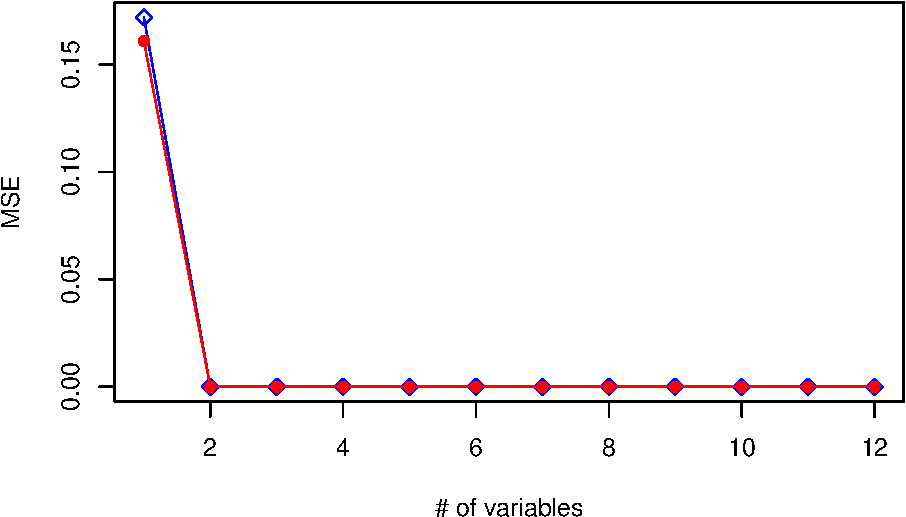
\includegraphics[keepaspectratio]{_main_files/figure-latex/unnamed-chunk-53-1.pdf}}

In this example both errors are very small which makes it hard to illustrate the differences in the two errors, but feel free to use this code in other examples to observe more patterns between training/testing errors.

In general, we expect that in each iteration, the blue line (representing the training error) consistently exhibits a monotonically decreasing trend, signifying the reduction of training error as more predictors are incorporated. On the other hand, the red line's (testing error) trajectory may not uniformly decrease.

\subsubsection{Test for Outliers}\label{test-for-outliers}

In this example, we check the data set for unusual observations. Specifically, we will check for:

To identify outliers, we use the Bonferroni test. For that purpose, we need to compute the studentized residuals \(t_{i}\) ( an externally standardized version of residuals ). Under the null hypothesis \(H_{0}\), \(t_{i} \sim t_{n-p}\), where \(n\) is the sample size and \(p\) is the number of predictors without the intercept. We perform this test for all \(n\) observations testing case at level \(\frac{\alpha}{n}\):

\begin{Shaded}
\begin{Highlighting}[]
\DocumentationTok{\#\# We work with the full model again.}
\NormalTok{n }\OtherTok{=} \FunctionTok{dim}\NormalTok{(birthweight)[}\DecValTok{1}\NormalTok{]; }
\NormalTok{p }\OtherTok{=} \FunctionTok{length}\NormalTok{(}\FunctionTok{variable.names}\NormalTok{(birthweight.mlr.full)); }
\end{Highlighting}
\end{Shaded}

We first compute the studentized residuals using the \texttt{rstudent} R function and the Bonferroni critical value using Student's distribution:

\begin{Shaded}
\begin{Highlighting}[]
\DocumentationTok{\#\# Computing Studentized Residuals \#}
\NormalTok{birthweight.resid }\OtherTok{=} \FunctionTok{rstudent}\NormalTok{(birthweight.mlr.full); }

\DocumentationTok{\#\# Critical value WITH Bonferroni correction \#}
\NormalTok{bonferroni\_cv }\OtherTok{=} \FunctionTok{qt}\NormalTok{(.}\DecValTok{05}\SpecialCharTok{/}\NormalTok{(}\DecValTok{2}\SpecialCharTok{*}\NormalTok{n), n}\SpecialCharTok{{-}}\NormalTok{p}\DecValTok{{-}1}\NormalTok{) }
\NormalTok{bonferroni\_cv}
\end{Highlighting}
\end{Shaded}

\begin{verbatim}
## [1] -3.60755
\end{verbatim}

Now, we need to find which (if any) studentized residuals exceed the Bonferroni critical value:

\begin{Shaded}
\begin{Highlighting}[]
\DocumentationTok{\#\# Sorting the residuals in descending order to find outliers (if any) }
\NormalTok{birthweight.resid.sorted }\OtherTok{=} \FunctionTok{sort}\NormalTok{(}\FunctionTok{abs}\NormalTok{(birthweight.resid), }\AttributeTok{decreasing=}\ConstantTok{TRUE}\NormalTok{)[}\DecValTok{1}\SpecialCharTok{:}\DecValTok{10}\NormalTok{]}
\FunctionTok{print}\NormalTok{(birthweight.resid.sorted)}
\end{Highlighting}
\end{Shaded}

\begin{verbatim}
##        2       29       34        1       28       20       42       24 
## 2.068621 1.890299 1.830714 1.682375 1.645611 1.613154 1.435773 1.411769 
##       19       39 
## 1.347956 1.324123
\end{verbatim}

\begin{Shaded}
\begin{Highlighting}[]
\NormalTok{birthweight.outliers }\OtherTok{=}\NormalTok{ birthweight.resid.sorted[}\FunctionTok{abs}\NormalTok{(birthweight.resid.sorted) }\SpecialCharTok{\textgreater{}} \FunctionTok{abs}\NormalTok{(bonferroni\_cv)]}
\FunctionTok{print}\NormalTok{(birthweight.outliers)}
\end{Highlighting}
\end{Shaded}

\begin{verbatim}
## named numeric(0)
\end{verbatim}

Above, we computed a t-value of \(|-3.61|\) at \(\alpha=0.05\). If an observation's studentized residual is higher (in absolute value) than the critical value of the \(T\) distribution with Bonferroni correction, then this observation will be considered an outlier. According to this criterion, we can see that \textbf{we don't have any outliers in the data set, since none of the studentized residuals is higher than \(|-3.61|\).}

\subsubsection{Checking Model Assumptions}\label{checking-model-assumptions}

We start by using residual plots and specifically the residuals against fitted values:

\begin{Shaded}
\begin{Highlighting}[]
\FunctionTok{plot}\NormalTok{(birthweight.mlr.full, }\AttributeTok{which=}\DecValTok{1}\NormalTok{)}
\end{Highlighting}
\end{Shaded}

\pandocbounded{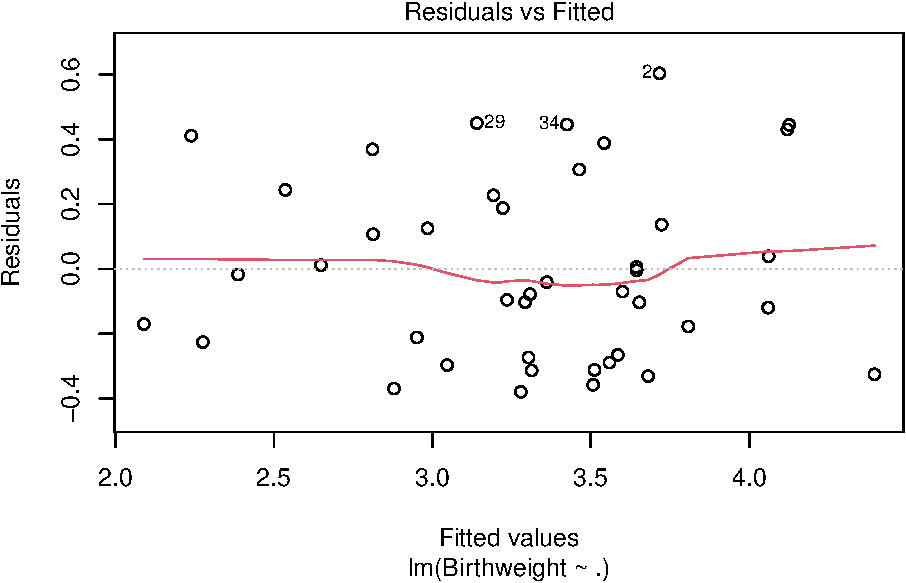
\includegraphics[keepaspectratio]{_main_files/figure-latex/unnamed-chunk-57-1.pdf}}

The points on the plot are randomly scattered around the zero line, so we conclude that the constant variance assumption is satisfied.

We continue by checking the normality assumption:

\begin{Shaded}
\begin{Highlighting}[]
\FunctionTok{plot}\NormalTok{(birthweight.mlr.full, }\AttributeTok{which=}\DecValTok{2}\NormalTok{)}
\end{Highlighting}
\end{Shaded}

\pandocbounded{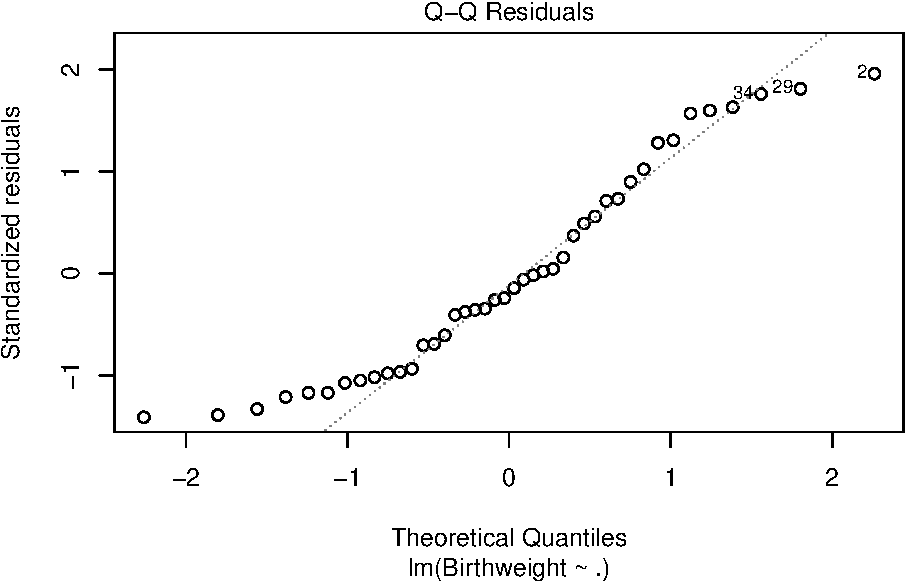
\includegraphics[keepaspectratio]{_main_files/figure-latex/unnamed-chunk-58-1.pdf}}

\begin{Shaded}
\begin{Highlighting}[]
\FunctionTok{hist}\NormalTok{(birthweight.mlr.full}\SpecialCharTok{$}\NormalTok{residuals)}
\end{Highlighting}
\end{Shaded}

\pandocbounded{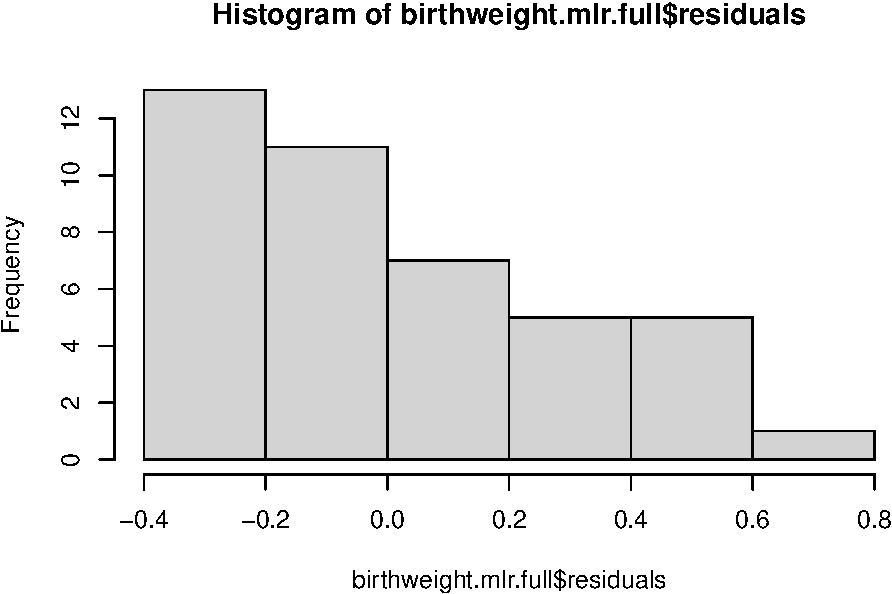
\includegraphics[keepaspectratio]{_main_files/figure-latex/unnamed-chunk-58-2.pdf}}

We seem to have some departures from the normality assumption in this case.

\subsubsection{Collinearity: Car Seat Position Data (a Faraway data set)}\label{collinearity-car-seat-position-data-a-faraway-data-set}

Car drivers like to adjust the seat position for their own comfort.
Car designers would find it helpful to know how different drivers
will position the seat depending on their \emph{size} and \emph{age.} Researchers
at the HuMoSim laboratory at the University of Michigan collected the following data on \textbf{38} drivers:

\texttt{Age}: Drivers age in years

\texttt{Weight}: Drivers weight in lbs

\texttt{HtShoes}: height with shoes in cm

\texttt{Ht}: height without shoes in cm

\texttt{Seated}: seated height in cm

\texttt{Arm}: lower arm length in cm

\texttt{Thigh}: thigh length in cm

\texttt{Leg}: lower leg length in cm

\texttt{hipcenter}: horizontal distance of the midpoint of the hips from a
fixed location in the car in mm

To read the data we need to load the \texttt{faraway} library and then open the \texttt{seatpos} data set.

\begin{Shaded}
\begin{Highlighting}[]
\FunctionTok{library}\NormalTok{(faraway)}
\FunctionTok{data}\NormalTok{(seatpos)}
\FunctionTok{attach}\NormalTok{(seatpos)}
\end{Highlighting}
\end{Shaded}

Let's start by fitting the \textbf{full} model with \texttt{hipcenter} as a response and everything else as a predictor:

\begin{Shaded}
\begin{Highlighting}[]
\CommentTok{\# Fit the FULL model}
\NormalTok{position.full}\OtherTok{=}\FunctionTok{lm}\NormalTok{(hipcenter }\SpecialCharTok{\textasciitilde{}}\NormalTok{ ., seatpos)}
\FunctionTok{summary}\NormalTok{(position.full)}
\end{Highlighting}
\end{Shaded}

\begin{verbatim}
## 
## Call:
## lm(formula = hipcenter ~ ., data = seatpos)
## 
## Residuals:
##     Min      1Q  Median      3Q     Max 
## -73.827 -22.833  -3.678  25.017  62.337 
## 
## Coefficients:
##              Estimate Std. Error t value Pr(>|t|)  
## (Intercept) 436.43213  166.57162   2.620   0.0138 *
## Age           0.77572    0.57033   1.360   0.1843  
## Weight        0.02631    0.33097   0.080   0.9372  
## HtShoes      -2.69241    9.75304  -0.276   0.7845  
## Ht            0.60134   10.12987   0.059   0.9531  
## Seated        0.53375    3.76189   0.142   0.8882  
## Arm          -1.32807    3.90020  -0.341   0.7359  
## Thigh        -1.14312    2.66002  -0.430   0.6706  
## Leg          -6.43905    4.71386  -1.366   0.1824  
## ---
## Signif. codes:  0 '***' 0.001 '**' 0.01 '*' 0.05 '.' 0.1 ' ' 1
## 
## Residual standard error: 37.72 on 29 degrees of freedom
## Multiple R-squared:  0.6866, Adjusted R-squared:  0.6001 
## F-statistic:  7.94 on 8 and 29 DF,  p-value: 1.306e-05
\end{verbatim}

Note that the \(p\)-value of the overall \(F\) test is very small (1.306e-05), which means that \emph{at least one of the predictors is statistically significant}, but at the same time none of the predictors is statistically significant according to the individual \(t\) tests. This is strange and definitely a \emph{red flag} that we may have collinearity issues.

To investigate the presence of high correlated predictors as well as the linear correlation of the response with each of the predictors, we start by checking the \textbf{correlation matrix}:

\begin{Shaded}
\begin{Highlighting}[]
\DocumentationTok{\#\# We use the round function with 2 digits, to round the numbers in the output}
\DocumentationTok{\#\# This only affects the printed numbers, not the ones R has stored.}
\FunctionTok{round}\NormalTok{(}\FunctionTok{cor}\NormalTok{(seatpos), }\AttributeTok{dig=}\DecValTok{2}\NormalTok{)}
\end{Highlighting}
\end{Shaded}

\begin{verbatim}
##             Age Weight HtShoes    Ht Seated   Arm Thigh   Leg hipcenter
## Age        1.00   0.08   -0.08 -0.09  -0.17  0.36  0.09 -0.04      0.21
## Weight     0.08   1.00    0.83  0.83   0.78  0.70  0.57  0.78     -0.64
## HtShoes   -0.08   0.83    1.00  1.00   0.93  0.75  0.72  0.91     -0.80
## Ht        -0.09   0.83    1.00  1.00   0.93  0.75  0.73  0.91     -0.80
## Seated    -0.17   0.78    0.93  0.93   1.00  0.63  0.61  0.81     -0.73
## Arm        0.36   0.70    0.75  0.75   0.63  1.00  0.67  0.75     -0.59
## Thigh      0.09   0.57    0.72  0.73   0.61  0.67  1.00  0.65     -0.59
## Leg       -0.04   0.78    0.91  0.91   0.81  0.75  0.65  1.00     -0.79
## hipcenter  0.21  -0.64   -0.80 -0.80  -0.73 -0.59 -0.59 -0.79      1.00
\end{verbatim}

We observe that the response is \emph{highly correlated with most of the variables} which justifies the low \(p\)-value in the overall \(F\) test. However, we have \textbf{highly correlated predictors} (e.g.~Corr(\texttt{Leg}, \texttt{HtShoes})=0.91) which means that we will have \emph{collinearity.}

Let's look at the \textbf{condition number} of the \(\mathbf{X}^T\mathbf{X}\) matrix. Recall that the condition number is \emph{not scale invariant}. This implies that calculating it before standardizing the matrix might lead to incorrect conclusions. So, let's standardize it first:

\begin{Shaded}
\begin{Highlighting}[]
\DocumentationTok{\#\# Extract the design matrix and remove the column of 1s that corresponds to the intercept.}
\NormalTok{x }\OtherTok{=} \FunctionTok{model.matrix}\NormalTok{(position.full)[,}\SpecialCharTok{{-}}\DecValTok{1}\NormalTok{]}

\DocumentationTok{\#\# Standardize the matrix}
\NormalTok{x }\OtherTok{=}\NormalTok{ x }\SpecialCharTok{{-}} \FunctionTok{matrix}\NormalTok{(}\FunctionTok{apply}\NormalTok{(x,}\DecValTok{2}\NormalTok{, mean), }\DecValTok{38}\NormalTok{,}\DecValTok{8}\NormalTok{, }\AttributeTok{byrow=}\ConstantTok{TRUE}\NormalTok{)}
\NormalTok{x }\OtherTok{=}\NormalTok{ x }\SpecialCharTok{/} \FunctionTok{matrix}\NormalTok{(}\FunctionTok{apply}\NormalTok{(x, }\DecValTok{2}\NormalTok{, sd), }\DecValTok{38}\NormalTok{,}\DecValTok{8}\NormalTok{, }\AttributeTok{byrow=}\ConstantTok{TRUE}\NormalTok{)}
\FunctionTok{apply}\NormalTok{(x,}\DecValTok{2}\NormalTok{,mean)}
\end{Highlighting}
\end{Shaded}

\begin{verbatim}
##           Age        Weight       HtShoes            Ht        Seated 
## -5.843279e-18  2.534522e-16  9.524545e-16  1.577685e-16 -1.079546e-15 
##           Arm         Thigh           Leg 
## -1.285521e-16  9.860533e-17 -1.029878e-16
\end{verbatim}

\begin{Shaded}
\begin{Highlighting}[]
\FunctionTok{apply}\NormalTok{(x,}\DecValTok{2}\NormalTok{,var)}
\end{Highlighting}
\end{Shaded}

\begin{verbatim}
##     Age  Weight HtShoes      Ht  Seated     Arm   Thigh     Leg 
##       1       1       1       1       1       1       1       1
\end{verbatim}

Compute the condition number using the standardized matrix:

\begin{Shaded}
\begin{Highlighting}[]
\DocumentationTok{\#\# Compute the eigenvalues of the matrix}
\NormalTok{eigenvalues.x }\OtherTok{=} \FunctionTok{eigen}\NormalTok{(}\FunctionTok{t}\NormalTok{(x) }\SpecialCharTok{\%*\%}\NormalTok{ x) }
\NormalTok{eigenvalues.x}\SpecialCharTok{$}\NormalTok{val}
\end{Highlighting}
\end{Shaded}

\begin{verbatim}
## [1] 209.90786979  45.76108236  17.15850736   8.91545889   7.18612386
## [6]   5.14944541   1.86274750   0.05876483
\end{verbatim}

\begin{Shaded}
\begin{Highlighting}[]
\DocumentationTok{\#\# Compute the condition number:}
\FunctionTok{sqrt}\NormalTok{(eigenvalues.x}\SpecialCharTok{$}\NormalTok{val[}\DecValTok{1}\NormalTok{]}\SpecialCharTok{/}\NormalTok{eigenvalues.x}\SpecialCharTok{$}\NormalTok{val[}\DecValTok{8}\NormalTok{])}
\end{Highlighting}
\end{Shaded}

\begin{verbatim}
## [1] 59.7662
\end{verbatim}

The condition number is \textbf{59.77}, larger than 30, so we conclude that \emph{collinearity is present}.

Let's also check the \textbf{Variance Inflation Factor (VIF)}:

\begin{Shaded}
\begin{Highlighting}[]
\DocumentationTok{\#\# Variance Inflation Factor (VIF)}
\FunctionTok{round}\NormalTok{(}\FunctionTok{vif}\NormalTok{(x), }\AttributeTok{dig=}\DecValTok{2}\NormalTok{)}
\end{Highlighting}
\end{Shaded}

\begin{verbatim}
##     Age  Weight HtShoes      Ht  Seated     Arm   Thigh     Leg 
##    2.00    3.65  307.43  333.14    8.95    4.50    2.76    6.69
\end{verbatim}

\begin{Shaded}
\begin{Highlighting}[]
\FunctionTok{sqrt}\NormalTok{(}\FloatTok{307.43}\NormalTok{)}
\end{Highlighting}
\end{Shaded}

\begin{verbatim}
## [1] 17.53368
\end{verbatim}

Note that the \emph{standard error} for the coefficient associated with \texttt{HtShoes} is \textbf{17.5 times larger} than it would have been without collinearity.

The next step is to \textbf{investigate which variable to remove}. To do so, we study the \emph{pairwise correlations} and perform \emph{partial \(F\)-tests} as follows:

\begin{Shaded}
\begin{Highlighting}[]
\FunctionTok{cor}\NormalTok{(Seated}\SpecialCharTok{+}\NormalTok{Thigh, Ht)}
\end{Highlighting}
\end{Shaded}

\begin{verbatim}
## [1] 0.9389819
\end{verbatim}

\begin{Shaded}
\begin{Highlighting}[]
\FunctionTok{cor}\NormalTok{(Seated}\SpecialCharTok{+}\NormalTok{Leg, Ht)}
\end{Highlighting}
\end{Shaded}

\begin{verbatim}
## [1] 0.965607
\end{verbatim}

\begin{Shaded}
\begin{Highlighting}[]
\FunctionTok{cor}\NormalTok{(Seated}\SpecialCharTok{+}\NormalTok{Arm, Ht)}
\end{Highlighting}
\end{Shaded}

\begin{verbatim}
## [1] 0.9465523
\end{verbatim}

\begin{Shaded}
\begin{Highlighting}[]
\NormalTok{position.red1 }\OtherTok{=} \FunctionTok{lm}\NormalTok{(hipcenter }\SpecialCharTok{\textasciitilde{}}\NormalTok{ Age }\SpecialCharTok{+}\NormalTok{ Weight }\SpecialCharTok{+}\NormalTok{ Ht }\SpecialCharTok{+}\NormalTok{ Seated, }\AttributeTok{data=}\NormalTok{seatpos)}
\FunctionTok{summary}\NormalTok{(position.red1)}
\end{Highlighting}
\end{Shaded}

\begin{verbatim}
## 
## Call:
## lm(formula = hipcenter ~ Age + Weight + Ht + Seated, data = seatpos)
## 
## Residuals:
##     Min      1Q  Median      3Q     Max 
## -90.869 -21.163  -3.144  26.773  59.423 
## 
## Coefficients:
##              Estimate Std. Error t value Pr(>|t|)   
## (Intercept) 478.65890  159.73362   2.997  0.00515 **
## Age           0.58396    0.42573   1.372  0.17943   
## Weight       -0.01535    0.31640  -0.049  0.96159   
## Ht           -4.99025    1.64389  -3.036  0.00466 **
## Seated        2.04632    3.41283   0.600  0.55287   
## ---
## Signif. codes:  0 '***' 0.001 '**' 0.01 '*' 0.05 '.' 0.1 ' ' 1
## 
## Residual standard error: 36.83 on 33 degrees of freedom
## Multiple R-squared:  0.6599, Adjusted R-squared:  0.6186 
## F-statistic: 16.01 on 4 and 33 DF,  p-value: 2.224e-07
\end{verbatim}

\begin{Shaded}
\begin{Highlighting}[]
\NormalTok{position.red2 }\OtherTok{=} \FunctionTok{lm}\NormalTok{(hipcenter }\SpecialCharTok{\textasciitilde{}}\NormalTok{ Ht, }\AttributeTok{data=}\NormalTok{seatpos)}
\FunctionTok{summary}\NormalTok{(position.red2)}
\end{Highlighting}
\end{Shaded}

\begin{verbatim}
## 
## Call:
## lm(formula = hipcenter ~ Ht, data = seatpos)
## 
## Residuals:
##     Min      1Q  Median      3Q     Max 
## -99.956 -27.850   5.656  20.883  72.066 
## 
## Coefficients:
##             Estimate Std. Error t value Pr(>|t|)    
## (Intercept) 556.2553    90.6704   6.135 4.59e-07 ***
## Ht           -4.2650     0.5351  -7.970 1.83e-09 ***
## ---
## Signif. codes:  0 '***' 0.001 '**' 0.01 '*' 0.05 '.' 0.1 ' ' 1
## 
## Residual standard error: 36.37 on 36 degrees of freedom
## Multiple R-squared:  0.6383, Adjusted R-squared:  0.6282 
## F-statistic: 63.53 on 1 and 36 DF,  p-value: 1.831e-09
\end{verbatim}

\begin{Shaded}
\begin{Highlighting}[]
\FunctionTok{anova}\NormalTok{(position.red2, position.red1)}
\end{Highlighting}
\end{Shaded}

\begin{verbatim}
## Analysis of Variance Table
## 
## Model 1: hipcenter ~ Ht
## Model 2: hipcenter ~ Age + Weight + Ht + Seated
##   Res.Df   RSS Df Sum of Sq      F Pr(>F)
## 1     36 47616                           
## 2     33 44774  3    2841.6 0.6981 0.5599
\end{verbatim}

Based on the \(F\) test provided in the ANOVA table, we conclude that \emph{the reduced model with \texttt{Ht} as the only variable is better than the model that includes \texttt{Age}, \texttt{Weight}, \texttt{Ht} and \texttt{Seated}}.

\chapter{Variable Selection \& Regularization}\label{variable-selection-regularization}

Let's consider the multiple linear regression model with \(p\) predictors \textbf{plus} the intercept, i.e.
\[Y \sim 1+ X_1+X_2+ \ldots+X_p\]

In many applications, the number of explanatory variables, i.e., \(p\) is large while in some cases we could even have \(p\gg n\). However, this does not necessarily mean that all the variables are relevant to the response \(Y\). In fact, \emph{only a small portion} of the \(p\) variables are believed to be relevant to \(Y\).

Our \textbf{goal} in this chapter is to develop methods that will allow us to efficiently identify the set of predictors that are useful in estimating or predicting the response. Since the least squares estimator \(\hat{\mathbf{\beta}}\) is \emph{unbiased}, this implies that irrelevant estimators \(\hat{\beta}_j\) will eventually go to zero. So, if our task is to do well on prediction, \emph{then we need to reflect on whether it is it important to remove unnecessary variables from the model}.

To better understand the implications of unnecessary parameters in a MLR model, we further discuss and quantify the \textbf{Training} and \textbf{Testing Errors} .

\section{Training vs.~Testing Errors}\label{training-vs.-testing-errors}

Consider that we \emph{split our data in two parts}:

\begin{itemize}
\item
  \textbf{Training data} \(\{\mathbf{x}_i, y_i \}_{i=1}^n\) are used to fit our model
\item
  \textbf{Testing data} \(\{\mathbf{x}_i, y_i^* \}_{i=1}^n\) are an \textbf{independent} data set collected at locations \(\mathbf{x}_i\)
\end{itemize}

\textbf{Remark}: In practice, we are given a full data set to analyze, which we then need to split it in two parts (typically in a random fashion) - a \emph{training} part and a \emph{testing} part with a higher percentage allocated to the training data (usually \textasciitilde80\%).

We assume that both \emph{testing} and \emph{training} data come from the same population or are collected at the same locations \(\mathbf{x}_i\). Then, \emph{statistically} we can write both models as follows:

\[\mathbf{y}_{n\times 1},\,\,  \mathbf{y}^*_{n\times 1}  \sim^{iid} N_n(\mathbf{\mu},\sigma^2 \mathbf{I}_n) \text{ and } \mathbf{\mu}=\mathbf{X}\mathbf{\beta}\]

or equivalently,

\[ \mathbf{y} = \mathbf{X}\mathbf{\beta} + \mathbf{\varepsilon},\, \mathbf{\varepsilon} \sim^{iid} \mathcal{N}_n(\mathbf{0},\sigma^2 \mathbf{I}_n) \quad \text{ and } \quad \mathbf{y}^* =\mathbf{X}\mathbf{\beta} + \mathbf{\varepsilon}^*,\, \mathbf{\varepsilon}^* \sim^{iid} \mathcal{N}_n(\mathbf{0},\sigma^2 \mathbf{I}_n) \]
\[ \text{ with }\,\, \mathbf{\varepsilon},  \mathbf{\varepsilon}^* \,\,  \text{ independent}.\]

Having these models in mind, we compute the \textbf{MSE for train and testing data}:

Note that for simplicity in the calculations below, we have suppressed the intercept (so there is no \(\beta_0\)). If we have an intercept, then instead of \(p\), we will have \(p+1\).

\begin{align*}
{\color{blue} {\mathbb{E}\bigl(\text{Train Error}\bigr)}} & =  \mathbb{E}\Bigl|\Bigl|\mathbf{y}-\hat{\mathbf{y}} \Bigr|\Bigr|^2=\mathbb{E}\Bigl|\Bigl|(\mathbf{I - H})\mathbf{y}\Bigr|\Bigr|^2\\
  &=tr \Bigl((\mathbf{I - H})Cov(\mathbf{y})(\mathbf{I - H})^T \Bigr)\\
  & = \sigma^2 tr\Bigl( (\mathbf{I - H}) \Bigr)=  (n-p) \sigma^2\\
  &= {\color{blue} {n\sigma^2 \mathbf{-} p \sigma^2}}\\
\end{align*}

\begin{align*}
{\color{blue} {\mathbb{E}\bigl(\text{Test Error} \bigr)}} & = \mathbb{E}\Bigl|\Bigl|\mathbf{y}^*-\mathbf{X}\hat{\mathbf{\beta}}\Bigr|\Bigr|^2\\
&= \mathbb{E}\Bigl|\Bigl|(\mathbf{y}^*- \mathbf{X} \mathbf{\beta})+(\mathbf{X} \mathbf{\beta}-\mathbf{X}\hat{\mathbf{\beta}})\Bigr|\Bigr|^2\\
&= \mathbb{E}\Bigl|\Bigl|\mathbf{y}^* -\mathbf{\mu}\Bigr|\Bigr|^2 + \mathbb{E}\Bigl|\Bigl|\mathbf{X} \mathbf{\beta}-\mathbf{X}\hat{\mathbf{\beta}}\Bigr|\Bigr|^2\\
&= \mathbb{E}||\mathbf{\varepsilon}^*||^2 + tr\Bigl(\mathbf{X}Cov(\hat{\mathbf{\beta}})\mathbf{X}^T \Bigr)\\
&= n \sigma^2 +\sigma^2 tr\mathbf{H}\\
&= {\color{blue} {n \sigma^2 \mathbf{+}  p \sigma^2}}\\
\end{align*}

From the previous equations we can conclude that:

\begin{itemize}
\item
  the \emph{training error decreases with \(p\)} .
\item
  the \emph{testing error increases with \(p\)} .
\end{itemize}

This implies that if our goal is \emph{pure prediction}, adding more variables to matrix \(\mathbf{X}\) is not the best option. But, \emph{does this imply that the intercept-only model with \(p=0\), i.e.~the one with the smallest expected test error is the best}? \textbf{No!}

The previous analysis is based on the following \textbf{Assumptions}:

\begin{enumerate}
\def\labelenumi{\arabic{enumi}.}
\item
  The mean of \(\mathbf{y}\), i.e.~\(E(\mathbf{Y}|\mathbf{X})\), is in \(\mathcal{C}(\mathbf{X})\), i.e., there exists some coefficient vector \(\mathbf{\beta}\) such that \(E(\mathbf{Y}|\mathbf{X}) = \mathbf{X}\mathbf{\beta}\).
\item
  The design matrix \(\mathbf{X}\) above contains all available predictors. But, when we run a linear regression model using only a \textbf{subset} of the columns of \(\mathbf{X}\), there will be \emph{an additional \textbf{Bias} term}.
\end{enumerate}

Even more generally, we may have a \emph{model}:
\[Y = f(X) + \varepsilon\]
in which \(f\) is not even linear. In such cases, we approximate \(f\) with a linear function \(f^*\) which means that we introduce bias. (Intuitively, this means that usually when we do not know the underlying true model, a linear approximation is often a good first step.) In the same spirit, even when the underlying function is truly linear, we may still introduce bias when we use a subset of the design matrix \(\mathbf{X}\), i.e.~when the model misses some relevant variables.

In such cases, the training and testing errors compute as:

\begin{align*}
\mathbb{E}\bigl(\text{Test Error}\bigr)^2 &= n\sigma^2 + \color{blue}{p\sigma^2} + \color{orange}{Bias}\\
\mathbb{E}\bigl(\text{Training Error}\bigr)^2 &= n\sigma^2 - \color{blue}{p\sigma^2} + \color{orange}{Bias}
\end{align*}
where \(p\sigma^2\) is the unavoidable error -- the \(\varepsilon\) -- and Bias is the model error.

\begin{itemize}
\item
  Bigger model (i.e., \(p\) large) \(\rightarrow\) small Bias, but large Variance (\(p\sigma^2\))
\item
  Smaller model (i.e., \(p\) small) \(\rightarrow\) large Bias, but small Variance (\(p\sigma^2\)).
\end{itemize}

To reduce the \emph{test error} (i.e., prediction error), the key is to find the best \textbf{trade-off} between Bias and Variance.

\section{Subset Selection}\label{subset-selection}

The idea behind \emph{subset selection} is to score each model according to an information criterion and then use a search algorithm to find the optimal model. In this way, we take into account

\[\text{Training Error + Complexity Penalty}\]

In the context of linear regression models, the \emph{complexity of a model increases with the number of predictor variables} (i.e., \(p\)).

\begin{itemize}
\item
  \textbf{Training Error}: an increasing function of \(RSS\).
\item
  \textbf{Complexity Penalty}: an increasing function of \(p\).
\end{itemize}

\begin{quote}
\emph{Why don't we just use \(R^2\) or \(RSS\)?} The main reason is that \(R^2\) always increases when we introduce variables in the model, while \(RSS\) always reduces. Therefore, \(R^2\) and \(RSS\) do not penalize for introducing unnecessary variables in the model.
\end{quote}

\subsection{Information Criteria-based procedures}\label{information-criteria-based-procedures}

\textbf{Akaike Information Criterion \& Bayesian Information Criterion}

\(AIC\) and \(BIC\) are defined as

\begin{align*}
AIC &= -2\cdot loglik  + 2\; p \\
BIC &= -2\cdot loglik  + \log(n)\; p
\end{align*}
where \(p\) is the number of predictors included in model under consideration. \(loglik\) denotes the log-likelihood of the model under consideration. For the normal-error linear regression model, the first term computes:
\[-2 \cdot  loglik = n\log \frac{RSS}{n} \]
which means that

\begin{align*}
AIC &= n\log \frac{RSS}{n} + 2\; p\\
BIC &= n\log \frac{RSS}{n} + \log(n)\; p
\end{align*}

The \textbf{lower} the AIC/BIC the \textbf{better}. Note that when \(n\) is large, \emph{adding an additional predictor costs a lot more in BIC than AIC}. So, AIC tends to pick a bigger model than BIC.

\textbf{Adjusted-\(R^2\) for model with \(p\) predictors}

\begin{align*}
R^2_a & = 1-\frac{RSS/(n-p-1)}{TSS/(n-1)}\\
& = 1- (1-R^2)\Bigl(\frac{n-1}{n-p-1}\Bigr)\\
& = {\color{blue}{1-\frac{\hat{\sigma}^2}{\hat{\sigma}^2_0}}}
\end{align*}
where \(\hat{\sigma}\) is the estimated error variance for the current fitted model, and \(\hat{\sigma}^2_0\) is the estimated error variance for the full fitted model.

The \textbf{higher} the \(R^2_a\) the \textbf{better}.

\textbf{Mallow's \(C_p\)}

\[C_p = \frac{RSS_{\mathbf{p}}}{\hat{\sigma}_0^2} +2p-n\]

where \(\hat{\sigma}_0^2\) is the estimate of the error variance for the full model.
Mallow's \(C_p\) behaves very similar to AIC and the \textbf{lower} the \(C_p\) the \textbf{better}.

\textbf{Illustration of Complexity Criteria vs.~\(p\)}

As an illustration, the complexity penalties \(R^2_{\text{adjusted}}\), Mallow's \(C_p\), \(AIC\), and \(BIC\) are plotted as a function of \(p\) (the number of parameters in the model) for the \texttt{student-grades} data set (the example in the last section):

\begin{figure}

{\centering 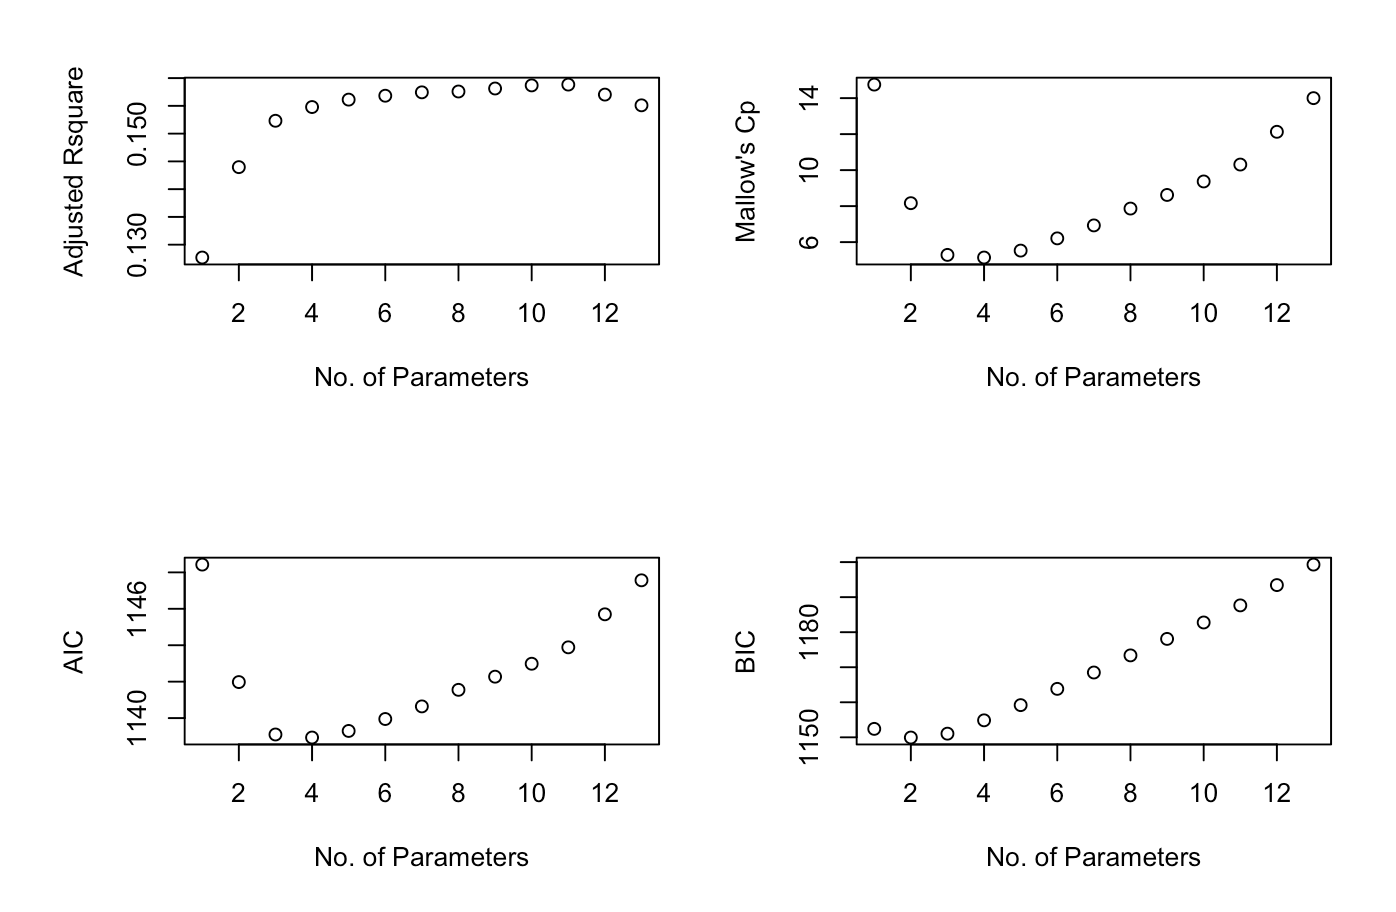
\includegraphics[width=0.95\linewidth]{images/week3/criteria} 

}

\caption{Subset selection criteria vs. p.}\label{fig:unnamed-chunk-66}
\end{figure}

\subsection{Search Algorithms}\label{search-algorithms}

In the beginning of this section, we discussed that to select the optimal model, we need to penalize the models using the preferred penalty. If we have (in total) \(p\) available predictors, then there are \(2^p\) potential models. Ideally, we would like to search and score all of these models. If \(p\) is large, then we need to employ systematic algorithms that search and score potential models.

\textbf{Level-wise search algorithms}: These are algorithms return the global optimal solution among \emph{all possible models} and work only for less than \emph{40} variables.

The idea is that they finds \(m\) different models (default \(m\) in \texttt{R} is 8) of up to size \(p\) with the smallest \(RSS\) among all the models of the same size. Then, they evaluate the score on the \(p\) models and report the optimal one. It is important to note that the algorithm does not need to visit every model. For example, if we know that \(RSS(X1, X2) < RSS(X3, X4, X5, X6)\), then it is not necessary to search any size 2 or 3 \emph{sub-models} of set \((X3, X4, X5, X6)\) meaning that these models may be leaped over.

\textbf{Greedy algorithms}: These algorithms add and/or remove variables based on the score given by a criterion such as AIC/BIC. They can move :

\begin{itemize}
\item
  \emph{Backwards}: start with the full model and sequentially delete predictors until the score does not improve.
\item
  \emph{Forward}: start with the null model and sequentially add predictors until the score does not improve.
\item
  \emph{Stepwise}: consider both deleting and adding one predictor at each stage.
\end{itemize}

These algorithms are computationally efficient, but they only return a \emph{locally optimal} solution which usually good enough in practice.

\subsubsection*{Some considerations}\label{some-considerations}
\addcontentsline{toc}{subsubsection}{Some considerations}

In some cases, specially when \(p\gg n\) starting with the full model and using the stepwise procedure is not feasible. Therefore, we need to screen some of the variables and remove them, before employing the search algorithms. A common variable screening approach is the following:

\begin{itemize}
\item
  Pick a \emph{smaller initial model} as a starting point by \textbf{ranking} the \(p\) predictors by the absolute value of their (marginal) correlation with \(Y\).
\item
  Keep the \textbf{top} \(K\) predictors (e.g., \(K = n/3\)).
\item
  Use the stepwise procedure so that you can add removed variables back to the model.
\end{itemize}

\section{Shrinkage Methods}\label{shrinkage-methods}

The variable selection methods we already discussed work quite well in practice when it comes to data sets where we do not have too many predictors. For example, recall that the \emph{level-wise} algorithms are good when \(p<40\).

In this section, we are going to study two different methods we can use to \textbf{shrink} the number of predictors in order to select the optimal model that balances the \emph{trade-off between model bias and prediction error (variance)}.

Let us then re-frame what we have been doing so far:

\textbf{Regression with Penalization}

\begin{align*}
\hat{\beta} &= \arg\min_{\beta} ||\mathbf{y} - \mathbf{X}\beta||^2 + \underbrace{\lambda \sum_{j=1}^{p} \mathbf{1}_{\beta_j \neq 0}}_{\text{penalty}}\\
&=  \arg\min_{\beta} ||\mathbf{y} - \mathbf{X}\beta||^2 + \underbrace{\lambda ||\beta||_0}_{\text{penalty}}
\end{align*}
where \(||\beta||_0 = \sum_{j=1}^{p} \mathbf{1}_{\beta_j \neq 0}\). The \emph{vector norm} \(||\beta||_0\) can be thought of as a function that decides whether a variable is \textbf{in} or \textbf{out} of the model. Then, the different criteria we discussed before rise by choosing \(\lambda\) properly.

Taking this idea one step further (remembering our linear algebra tools), we can replace the \emph{0-norm} above with a different one, e.g.~the \(L^1\) or the \(L^2\) norm. Exactly this observation, lead to two extremely popular \emph{penalized regression} methods:

\begin{itemize}
\item
  the \textbf{Ridge Regression}
  \[\hat{\beta} =  \arg\min_{\beta} ||\mathbf{y} - \mathbf{X}\beta||^2 + \underbrace{\lambda ||\beta||^2}_{\text{penalty}}, \text{ where } ||\beta||^2 = \sum_{j=1}^{p} \beta_j^2\]
\item
  the \textbf{Lasso Regression}
  \[\hat{\beta} =  \arg\min_{\beta} ||\mathbf{y} - \mathbf{X}\beta||^2 + \underbrace{\lambda |\beta|}_{\text{penalty}}, \text{ where }  |\beta| = \sum_{j=1}^{p} |\beta_j|\]
\end{itemize}

In the next sections, we discuss the mathematics and the implementation of these methods. However, before proceeding, we need to make two consider the following:

\textbf{Implementation Considerations}

When the penalization norm changes, we observe that the penalty term that arises (in both cases) \emph{is not location or scale invariant}. This implies that if we re-scale a variable then the penalized \(\beta\) estimators will be sensitive to these values. Therefore, it is suggested that we \textbf{center} and \textbf{scale} each column of the design matrix \(\mathbf{X}\). Specifically, if \(\mathbf{x}_{j}\), \(j=1, \ldots, p\) is a column of \(\mathbf{X}\), then
\[\tilde{\mathbf{x}}_{j} = \frac{ \mathbf{x}_{j} - \bar{\mathbf{x}}_{j} } { sd_{\mathbf{x}_{j}}} \]
In addition to that we \textbf{center} \(\mathbf{y}\) to \emph{suppress the intercept}, i.e.~\[\mathbf{\tilde{y}}_i = \mathbf{y}_{i} - \bar{\mathbf{y}}\]

After the model selection/fitting, we can always transform the variables back to their original values so that we continue with interpretation and/or prediction. We can also \emph{estimate back the intercept} as follows:

\[\hat{\beta}_0 = \bar{y} - \sum_{j=1}^{n} \hat{\beta}_j \bar{\mathbf{x}}_{j} \]

Note that in \texttt{R} tha \texttt{glmnet} package handles the centering and scaling (and transformation back to original) automatically.

\subsection{Ridge Regression}\label{ridge-regression}

Ridge regression assumes that after normalization, some of the regression coefficients should not be very large. Ridge regression is very useful when you have collinearity and the LS regression coefficients are unstable. In fact, it was initially introduced by A. Tikhonov to remedy multi-collinearity problems by adding a non-negative constant to the diagonal of the design matrix.

\textbf{Ridge Regression}

The idea of the method is to add a \textbf{penalty} term to the LS minimization problem :
\[\text{minimize}_{\beta}\,  (y-X \beta)^T(y-X \beta) + {\color{blue}{\lambda \sum_j \beta_j^2}}\]
for some \(\lambda \ge 0\). The penalty term is \(\sum_j \beta_j^2\).

As discussed before, for the method to be more effective, we prefer to \emph{standardize} the predictors first (centered by their means and scaled by their standard deviations) and center the response \(y\).

One of the main advantages of the ridge regression is that it provides us with closed-form solutions for the \(\beta\) coefficients. Indeed, solving the minimization problem we obtain:
\[\hat{\beta}_{\text{Ridge}}=(X^T X+\underbrace{\lambda I}_{\text{ridge}})^{-1} X^T y\]

It is easy to see that when \(\lambda=0\) the ridge regression estimation problem reduces to the standard least squares problem, while when \(\lambda \rightarrow \infty\), the ridge coefficients \(\hat{\beta} \rightarrow \mathbf{0}\). As a result, during implementation, one of the main considerations is how to choose \(\lambda\). Choosing a very small (relatively speaking) value for \(\lambda\) leads back to the usual LS estimators, while choosing a very large value for \(\lambda\) makes most estimators zero.

To balance this trade-off in practice, a common approach is to use automated methods such as \emph{Generalized Cross-Validation} (GCV). The main \emph{disadvantage} of the ridge regression estimators is that they are \textbf{biased}, that is \(\mathbb{E}(\hat{\beta}) = \beta + \text{ bias}\).

To better understand the structure of the ridge regression LS Coefficients, assume that \(\mathbf{X}^T\mathbf{X} = \mathbf{I}_p\), that is the columns of the design matrix are orthogonal. Then, the general formula above reduces to
\[\hat{\beta}_{ridge} = \bigl(\mathbf{X}^T \mathbf{X} + \lambda I \bigr)^{-1} \mathbf{X}^T \mathbf{y} = \frac{1}{1+\lambda} \mathbf{X}^T \mathbf{y}\]
Similarly, the fitted values
\[\hat{\mathbf{y}}_{ridge} = \mathbf{X} \hat{\beta}_{ridge} = \frac{1}{1+\lambda}\; \hat{\mathbf{y}}_{LS} \]

If the columns of the design matrix are not orthogonal, then we can run the regression against an orthonormal version of \(\mathbf{X}\), known as \emph{principal components analysis}, or \emph{singular value decomposition}.

\subsubsection*{Singular Value Decomposition (SVD)}\label{singular-value-decomposition-svd}
\addcontentsline{toc}{subsubsection}{Singular Value Decomposition (SVD)}

The Singular Value Decomposition (SVD) is one of the most important concepts in applied mathematics. It is used for a number of application including dimension reduction and data analysis. Principal Components Analysis (PCA) is also a special case of the SVD.

\textbf{SVD of \(\mathbf{X}_{n\times p}\)}

Consider the design matrix \(\mathbf{X}_{n\times p}\). Then, \(\mathbf{X}\) can be written as
\[\mathbf{X} = \mathbf{U}_{n\times p} \; \mathbf{D}_{p\times p}\, \mathbf{V}_{p\times p}^T\]

where

\begin{itemize}
\item
  \(\mathbf{U}_{n\times p}\) orthogonal matrix with columns that are spanning \(\mathcal{C}(\mathbf{X})\).
\item
  \(\mathbf{V}_{p\times p}\) orthogonal matrix with columns that are spanning \(\mathbb{R}^p\).
\item
  \(\mathbf{D}_{p\times p}\) diagonal values with \(d_1 \geq \ldots \geq d_p \geq 0\) the singular values of \(\mathbf{X}\). If one or more \(d_j = 0\), then \(\mathbf{X}\) is singular, i.e.~not full-rank.
\end{itemize}

This factorization of the matrix \(\mathbf{X}\) is called the \textbf{singular value decomposition of} \(\mathbf{X}\), and the columns of \(\mathbf{U}\) and \(\mathbf{V}\) are called the left- and right-hand \textbf{singular vectors} of \(\mathbf{X}\).

For simplicity in the discussion, let \(n>p\) and \(rank(\mathbf{X}) = p\), which also implies that \(d_p>0\).

\textbf{Some Useful Properties of the SVD}

\begin{enumerate}
\def\labelenumi{\arabic{enumi}.}
\item
  The left-hand singular vectors are a set of orthonormal eigenvectors for \(\mathbf{X}^T\mathbf{X}\), i.e.~\(\mathbf{U}^T\mathbf{U} = \mathbf{I}\).
\item
  The right-hand singular vectors are a set of orthonormal eigenvectors for \(\mathbf{X}\mathbf{X}^T\), i.e.~\(\mathbf{V}^T\mathbf{V}=\mathbf{I}\).
\item
  The eigenvectors \(\mathbf{v}_j\) are also called the \emph{principal components directions} of the columns of \(\mathbf{X}\).
\item
  The first principal component direction \(v_1\) has the property that \(z_1 = \mathbf{X} \mathbf{v}_1 = \mathbf{u}_1 d_1\) has the largest sample variance among all normalized linear combinations of the columns of \(\mathbf{X}\).
\item
  The singular values are the square roots of the eigenvalues for \(\mathbf{X}^T\mathbf{X}\) and \(\mathbf{X}\mathbf{X}^T\), since these matrices have the same eigenvalues.
\item
  The first singular value is equal to
  \[\sigma_1 = \max_{||x||=1} ||\mathbf{X}||_2\]
\end{enumerate}

One of the goals of \emph{principal components analysis} is to find the new coordinates, or \emph{scores}, of the data in the principal components basis. If the original (centered or standardized) data was contained in the matrix \(\mathbf{X}\) and the eigenvectors of the covariance/correlation matrix \((\mathbf{X}^T\mathbf{X})\) were columns of a matrix \(\mathbf{V}\), then to find the scores (\(\mathbf{S}\) ) of the observations on the eigenvectors we can use the following equation:
\[\mathbf{X} = \mathbf{S} \mathbf{V}^T\]
where each columns of \(\mathbf{S}_{n\times p} = \mathbf{U}\mathbf{D}\) is the
so-called \textbf{principal component} and each column of \(V\) is the \textbf{principal
component direction} of \(\mathbf{X}\).

\subsubsection*{SVD of Fitted Values: LS vs.~Ridge}\label{svd-of-fitted-values-ls-vs.-ridge}
\addcontentsline{toc}{subsubsection}{SVD of Fitted Values: LS vs.~Ridge}

To observe how the \emph{ridge} affects the structure of the fitted \(\beta\), we have the following.

\begin{itemize}
\tightlist
\item
  In \emph{least-squares} regression, the fitted values compute as:
\end{itemize}

\begin{align*}
{\color{blue}{\hat{\mathbf{y}}_{LS}}} &= \mathbf{X} \hat{\beta}_{LS}= \mathbf{X} \bigl(\mathbf{X}^T \mathbf{X} \bigr)^{-1} \mathbf{X}^T \mathbf{y}\\
&= \mathbf{U} \; \mathbf{D}\; \mathbf{V}^T \bigl(\mathbf{V}\; \mathbf{D}^2\; \mathbf{V}^T\bigr)^{-1} \mathbf{V}\; \mathbf{D}\;\mathbf{U}^T \mathbf{y}\\
&= \mathbf{U} \; \mathbf{D}\; \mathbf{V}^T \bigl( \mathbf{V}^T \bigl)^{-1}\; \mathbf{D}^{-2}\; \mathbf{V}^{-1} \mathbf{V}\; \mathbf{D}\;\mathbf{U}^T \mathbf{y}\\
&= \mathbf{U} \; \mathbf{D}\; \mathbf{D}^{-2}\mathbf{D}\;\mathbf{U}^T \mathbf{y}\\
&= {\color{blue}{\mathbf{U} \mathbf{U}^T \mathbf{y}}}\\
&= {\color{blue}{\sum_{j=1}^{p} \bigl(\mathbf{u}_j^T \mathbf{y} \bigr) \mathbf{u}_{j}}}
\end{align*}
where we used the facts that \(\mathbf{U}^T \mathbf{U} =\mathbf{I}\), and that
\[\mathbf{X}^T \mathbf{X} = \mathbf{V}\; \mathbf{D}^T\;\mathbf{U}^T \mathbf{U} \; \mathbf{D}\; \mathbf{V}^T = \mathbf{V}\; \mathbf{D}^2\; \mathbf{V}^T\]
The last expression is the \emph{eigen-decomposition of \(\mathbf{X}^T \mathbf{X}\)}.

Similarly, for the ridge regression coefficients, we have:

\begin{align*}
{\color{blue}{\hat{\mathbf{y}}_{ridge}}} &= \mathbf{X} \hat{\beta}_{ridge}\\
&= \mathbf{X} \bigl(\mathbf{X}^T \mathbf{X} + \lambda \mathbf{I} \bigr)^{-1} \mathbf{X}^T \mathbf{y}\\
&= \mathbf{U}\;\mathbf{D}\;\mathbf{V}^T \bigl(  \mathbf{V}\; \mathbf{D}^2\; \mathbf{V}^T + \lambda \mathbf{I} \bigr)^{-1}\mathbf{V}\;\mathbf{D}\;\mathbf{U}^T  \mathbf{y}\\
&= \mathbf{U}\;\mathbf{D}\;\mathbf{V}^T \bigl(  \mathbf{V}\; \mathbf{D}^2\; \mathbf{V}^T + \lambda \mathbf{V}\mathbf{V}^T \bigr)^{-1}\mathbf{V}\;\mathbf{D}\;\mathbf{U}^T  \mathbf{y}\\
&= \mathbf{U}\;\mathbf{D}\;\mathbf{V}^T \bigl(  \mathbf{V}\; \bigl( \mathbf{D}^2 + \lambda \mathbf{I} \bigr)\;  \mathbf{V}^T \bigr)^{-1}\mathbf{V}\;\mathbf{D}\;\mathbf{U}^T  \mathbf{y}\\
&= \mathbf{U}\;\mathbf{D}\;\mathbf{V}^T (\mathbf{V}^T)^{-1}\; \bigl( \mathbf{D}^2 + \lambda \mathbf{I} \bigr)^{-1}\;  \mathbf{V}^{-1}\mathbf{V}\;\mathbf{D}\;\mathbf{U}^T  \mathbf{y}\\
&= {\color{blue}{\mathbf{U}\mathbf{D}\;\bigl( \mathbf{D}^2 + \lambda \mathbf{I} \bigr)^{-1}\; \mathbf{D}\mathbf{U}^T  \mathbf{y}}}
\end{align*}

In this last expression, note that

\begin{itemize}
\item
  \(\mathbf{D}\;\bigl( \mathbf{D}^2 + \lambda \mathbf{I} \bigr)^{-1}\) is a diagonal matrix with elements given by \(\frac{d_j^2}{d_j^2 + \lambda}\).
\item
  the vector \(\mathbf{U}^T  \mathbf{y}\) is the coordinates of the vector \(\mathbf{y}\) in the basis spanned by the \(p\) columns of \(\mathbf{U}\).
\end{itemize}

Therefore, \(\hat{\mathbf{y}}_{ridge}\) simplifies to
\[{\color{blue}{\hat{\mathbf{y}}_{ridge} = \sum_{j=1}^{p} \mathbf{u}_j \;  \frac{d_j^2}{d_j^2 + \lambda}  \; \mathbf{u}_j^T \mathbf{y}}}\]

As we can observe, the inner products \(\mathbf{u}_j^T \mathbf{y}\) are scaled by the factors \(\frac{d_j^2}{d_j^2 + \lambda}\), or in other words the ridge estimate \(\hat{\beta}_{ridge}\) \textbf{shrinks the LS estimate \(\hat{\beta}_{LS}\) by a factor of \(\frac{d_j^2}{d_j^2 + \lambda}\)} where \emph{the smaller the eigenvalues the more the shrinkage}. Essentially, ridge regression projects \(\mathbf{y}\) onto the principal components, and then shrinks the coefficients of the low--variance components more than the high-variance components.

\subsubsection*{Complexity of Ridge Regression}\label{complexity-of-ridge-regression}
\addcontentsline{toc}{subsubsection}{Complexity of Ridge Regression}

To quantify the complexity of a model, heuristically we need to understand the number of coefficients that need to be estimated. So, a linear regression model is a model with \(p\) covariates and \(p\) \(\beta\) coefficients, so it has \(p\) degrees of freedom. In ridge regression however, the estimated \(\beta\)s are still \(p\)-dimensional, however the method does not use all strength of the \(p\) covariates due to shrinkage. If \(\lambda\) is extremely large, there will be no effective covariates left in the model, meaning that they should all be close to zero. On the other hand, if \(\lambda\) is 0, then we go back to linear regression with \(p\) covariates and \(p\) degrees of freedom. So, in the case of the ridge regression, the truth lies somewhere between 0 and \(p\).

Let's formalize the intuition, by recalling that one method to compute the degrees of freedom of a model is to relate them to the correlation between the observed and fitted values as follows:
\[df = \sum_{i=1}^{n} Cor \bigl(y_i,\; \hat{y}_i \bigr)\]

\begin{itemize}
\tightlist
\item
  \textbf{Linear regression}:
  We have already shown that the fitted values can be expressed as \(\hat{\mathbf{y}} = \mathbf{H} \mathbf{y}\), in which case
  \[df = \sum_{i=1}^{n} Cor \bigl(y_i,\; \hat{y}_i \bigr) = \sum_{i=1}^{n} H_{ii} = tr \bigl( \mathbf{H} \bigr) = p\]
  where (recall) \(\mathbf{H}\) is the hat (projection) matrix equal to \(\mathbf{X} \bigl( \mathbf{X}^T \mathbf{X} \bigr)^{-1} \mathbf{X}^T \mathbf{y}\).
\end{itemize}

\begin{itemize}
\tightlist
\item
  \textbf{Ridge regression}:
  We have shown that \(\hat{y} = \underbrace{ \mathbf{X} \bigl(\mathbf{X}^T \mathbf{X} + \lambda \mathbf{I} \bigr)^{-1} \mathbf{X}^T}_{:= \mathbf{S}_{\lambda}} \mathbf{y} = \mathbf{S}_{\lambda}\mathbf{y}\). So, the effective degrees of freedom of the ridge regression are
\end{itemize}

\begin{align*}
df(\lambda) &= \sum_{i=1}^{n} Cor \bigl(y_i,\; \hat{y}_i \bigr) = \sum_{i=1}^{n} [S_{\lambda}]_{ii}\\
&= tr(\mathbf{S}_{\lambda}) \\
&=  tr(\mathbf{X} \bigl(\mathbf{X}^T \mathbf{X} + \lambda \mathbf{I} \bigr)^{-1} \mathbf{X}^T)\\
&= tr\Biggl( \sum_{j=1}^{p} \frac{d_j^2}{d_j^2 + \lambda} \mathbf{u}_i \mathbf{u}_i^T\Biggr) =  \sum_{j=1}^{p} \frac{d_j^2}{d_j^2 + \lambda}   
\end{align*}
Based on the expression above, we can see that the degrees of freedom of the ridge regression are a \emph{decreasing} function of \(\lambda\), and reduce to \(p\) when \(\lambda = 0\). One important consequence of this expression is that we can use it to determine the values of \(\lambda\) to use when applying cross validation. This can be done by thinking \(df(\lambda)\) as a function of \(\lambda\) and then setting \(df(\lambda)=k\), with \(k=1, \ldots, p\) representing all possible dfs. Then, we can solve with respect to \(\lambda\) using a numerical approach.

\subsection{Lasso Regression}\label{lasso-regression}

Lasso Regression is similar to the Ridge regression in the sense that it minimizes the least squares criterion \emph{subject to a penalty term}. However, the penalty term is different in the case of lasso.

\textbf{Lasso Regression}

\(\hat{\beta}_{\text{LASSO}}\) minimizes:
\[\text{minimize } (y-X \beta)^T (y-X\beta) + \lambda \sum_j |\beta_j|\]
for some \(\lambda \ge 0\). The penalty term is \(\sum_j |\beta_j|\) (\(L_1\) constraint).

In two-dimensions the constraint defines a square, while in higher dimensions it defines a polytope. Lasso is useful when the response can be explained by \emph{few} predictors with zero effect on the remaining predictors (Lasso is similar to a variable selection method). When \(\beta_j=0\) the corresponding predictor is eliminated which is not the case for ridge regression. Therefore, we use lasso when the effect of predictors is \textbf{sparse}. This means that only few predictors will have an effect on the response (e.g.~gene expression data) or when number of predictors is large (\(p>n\)).

The lasso solution is defined as
\[\hat{\beta}_{lasso} = \arg \min_{\beta\in \mathbb{R}^{p}} \Bigl((y-X\boldsymbol{\beta})^\top(y-X\boldsymbol{\beta}) + \lambda \sum_j |\beta_j| \Bigr)\]
and does not have a closed form expression.

If we assume that \(\mathbf{X}^T\mathbf{X} = \mathbf{I}_p\)\}, then
\begin{align*}
||\mathbf{y} - \mathbf{X}\beta||^2 &= ||\mathbf{y} - \mathbf{X}\hat{\beta}_{LS} + \mathbf{X}\hat{\beta}_{LS} - \mathbf{X}\beta||^2\\
&=||\mathbf{y} - \mathbf{X}\hat{\beta}_{LS}||^2 + ||\mathbf{X}\hat{\beta}_{LS} - \mathbf{X}\beta||^2
\end{align*}
where
\[2  \bigl( \mathbf{y} - \mathbf{X}\hat{\beta}_{LS}\bigr)^T \bigl(  \mathbf{X}\hat{\beta}_{LS} - \mathbf{X}\beta \bigr) = 2 \; r^T \; \bigl(  \mathbf{X}\hat{\beta}_{LS} - \mathbf{X} \beta\bigr) =0\]
since the swecond term is a linear combination of columns of \(\mathbf{X}\) no matter what value \(\beta\) takes, and thus is in \(\mathcal{C}(\mathbf{X})\), therefore orthogonal to the residual vector \(r\).

\subsubsection*{Obtaining the Lasso Solution}\label{obtaining-the-lasso-solution}
\addcontentsline{toc}{subsubsection}{Obtaining the Lasso Solution}

Although we do not have a closed form solution in the case of lasso, the minimization problem we have to solve is not very challenging.

The lasso solution can be expressed as:

\begin{align*}
\hat{\beta}_{lasso} &= \arg \min_{\beta\in \mathbb{R}^{p}} \Bigl( ||\mathbf{y}-\mathbf{X} \beta||^2 + \lambda |\beta| \Bigr)\\
&= \arg \min_{\beta\in \mathbb{R}^{p}} \Bigl( ||\mathbf{X} \hat{\beta}_{LS} -\mathbf{X} \beta||^2 + \lambda |\beta| \Bigr)\\
&= \arg \min_{\beta\in \mathbb{R}^{p}} \Bigl( \bigl(  \hat{\beta}_{LS} - \beta \bigr)^T \mathbf{X}^T \mathbf{X}  \bigl(  \hat{\beta}_{LS} - \beta \bigr) + \lambda |\beta| \Bigr)\\
&= \arg \min_{\beta\in \mathbb{R}^{p}} \Bigl( \bigl(  \hat{\beta}_{LS} - \beta \bigr)^T  \bigl(  \hat{\beta}_{LS} - \beta \bigr) + \lambda |\beta| \Bigr)\\
&= \arg \min_{\beta_1, \ldots, \beta_p} \sum_{i=1}^{p}  \Bigl( \bigl(  \beta_{j} - \hat{\beta}_{(LS)j} \bigr)^2  + \lambda |\beta_j| \Bigr)\\
\end{align*}

We can find the \emph{optimal} \(\beta_j\) for each of \(j=1, \ldots, p\) \textbf{separately} by solving the following generic problem for each dimension:

\[\arg \min_{x} \bigl( x-a \bigr )^2 + \lambda |x|,\,\, \lambda >0\]

Therefore, to solve the one-dim lasso above, define
\[f(x)  = \bigl( x-a \bigr )^2 + \lambda |x|,\,\, a\in\mathbb{R},\,\,\lambda >0\]

The value \(x^*\) that minimizes \(f(x)\) must satisfy:
\begin{align*}
\frac{\partial}{\partial x} \bigl(x^* - a \bigr)^2 + \lambda \;\frac{\partial}{\partial x} |x^*| & = 0\\
2\bigl(x^* - a \bigr) +\lambda z^* &= 0
\end{align*}
where \(z^*\) is the \emph{sub-gradient} of the absolute value function evaluated at \(x^*\), which equals to \(sign(x^*)\) if \(x^*\neq 0\) and any number in {[}-1,1{]}, if \(x^*=0\).

Therefore, the minimizer of \(f(x)\) is given by
\[x^* = S_{\lambda/2}(a) = sign(a) \bigl(|a|-\lambda/2 \bigr)_{+} = 
\begin{cases}
& a-\lambda/2,  \text{ if } \,\,  a \; >\lambda/2\\
& 0, \qquad \quad \text{ if } |a| \leq \lambda/2\\
& a+\lambda/2,  \text{ if } \,\,  a \; < -\lambda/2\\
\end{cases}
\]
where \(S_{\lambda/2}(\cdot)\) is often referred to as the \textbf{soft-thresholding operator}.

When the design matrix \(\mathbf{X}\) is orthogonal, the lasso solution simplifies to

\[\hat{\beta}_{j}^{lasso} = \begin{cases}
& sign (\hat{\beta}_{(LS)j} - \lambda/2), \text{ if }|\hat{\beta}_{(LS)j}| > \lambda/2\\
& 0, \text{ if }|\hat{\beta}_{(LS)j}| \leq \lambda/2\\
\end{cases}
\]

A large \(\lambda\) will cause some of the coefficients to be exactly zero. So, lasso does both variable (subset) selection and (soft) shrinkage.

\textbf{Remarks}

\begin{itemize}
\item
  It is suggested to use lasso when the effect of predictors is \emph{sparse}, since lasso will ``make'' some of the \(\beta\) coefficients zero keeping the coefficients that will have an effect on \(\mathbf{y}\). This is the reason why this method also works when the number of predictors is larger than the sample size (\(p>n\)). These are scenarios often encountered in genomic or proteomic data where the design matrices tend to have a lot of zeros and too many predictors.
\item
  In lasso as in ridge regression, we can select \(\lambda\) using Cross-Validation (CV). When \(\lambda\) increases, the number of predictors decreases.
\end{itemize}

\textbf{Comparing Ridge Regression and Lasso}

Lasso selects a sub-set of predictors (some coefficients will equal to zero), while ridge regression performs better when the response is a function of many predictors with coefficients around the same size. Lasso will perform better when a relatively small number of predictors have large coefficients and the rest are very small or equal to zero.Since the number of predictors is never known \emph{a priori}, cross-validation can be used to decide which approach is better for a particular data set.

Ridge regression does a proportional shrinkage. Lasso translates each
coefficient by a constant factor λ, truncating at zero.

\begin{figure}

{\centering 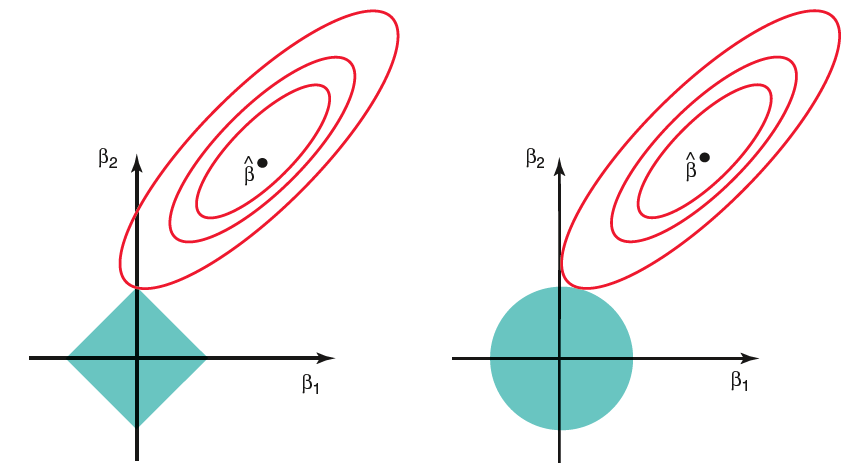
\includegraphics[width=0.75\linewidth]{images/week3/ridge-lasso_comparisson} 

}

\caption{Contour of the optimization for Lasso (left) and Ridge (right).}\label{fig:unnamed-chunk-67}
\end{figure}

In the picture below, we can see the difference in the contours of optimization for lasso (left) and Ridge (right) when there are only two parameters. The residual sum of squares has elliptical contours, centered at the full least squares estimate, \(\hat{\beta}_{LS}\). The constraint region for ridge regression is the disk \(\beta_1^2 + \beta_2^2 \leq t\), while that for lasso is the diamond \(|\beta_1| + |\beta_2| \leq t\). Both methods find the first point where the elliptical contours hit the constraint region. Unlike the disk, the diamond has corners which means that if the solution occurs at a corner, then it has one parameter
\(\beta_j\) equal to zero. When \(p>2\), the diamond becomes a rhomboid, and has many corners, flat edges and faces; there are many more opportunities for the estimated parameters to be zero.

\subsubsection*{\texorpdfstring{Lasso with \(p>n\)}{Lasso with p\textgreater n}}\label{lasso-with-pn}
\addcontentsline{toc}{subsubsection}{Lasso with \(p>n\)}

\emph{When \(\mathbf{X}\) is of full rank:}

\begin{itemize}
\item
  the lasso solution is the minimizer of a convex function over a convex set
\item
  the lasso solution is unique since the first term is a strictly convex function.
\end{itemize}

\emph{When \(\mathbf{X}\) is not of full rank, or when \(p>n\):}

\begin{itemize}
\tightlist
\item
  The lasso criterion is no longer convex which means that it may not have a unique minimizer.first term is no longer strictly convex. In the \(p>n\) case, the lasso selects at most \(n\) variables before it saturates, because of the nature of the convex optimization problem which is a limiting feature for a variable selection method.
\end{itemize}

\section{\texorpdfstring{The \texttt{Student\ Performance} Example}{The Student Performance Example}}\label{the-student-performance-example}

The \texttt{student-mat.csv} data set contains data from a study on student achievement in secondary education of two Portuguese schools. The data are based on the following publication:

\begin{quote}
``Using data mining to predict secondary school student performance''
By P. Cortez, A. M. G. Silva. 2008. Published in Proceedings of 5th Annual Future Business Technology Conference.
\end{quote}

and can be found in the UCI data repository: here

The variables in the data set are the following:

\begin{itemize}
\tightlist
\item
  \texttt{school} Student's school (\emph{binary}: \texttt{GP} - Gabriel Pereira or \texttt{MS} - Mousinho da Silveira)
\item
  \texttt{sex} Sex student's sex (\emph{binary}: \texttt{F} - female or \texttt{M} - male)
\item
  \texttt{age} Student's age (\emph{numeric}: from 15 to 22)
\item
  \texttt{address} Student's home address type (\emph{binary}: \texttt{U} - urban or \texttt{R} - rural)
\item
  \texttt{famsize} Family size (\emph{binary}: \texttt{LE3} - less or equal to 3 or \texttt{GT3} - greater than 3)
\item
  \texttt{Pstatus} Parent's cohabitation status (\emph{binary}: \texttt{T} - living together or \texttt{A} - apart)
\item
  \texttt{Medu} Μother's education level (\emph{numeric}: \texttt{0} - none, \texttt{1} - primary education (4th grade), \texttt{2} - 5th to 9th grade, \texttt{3} - secondary education or \texttt{4} - higher education)
\item
  \texttt{Fedu} Father's education level (\emph{numeric}: \texttt{0} - none, \texttt{1} - primary education (4th grade), \texttt{2} 5th to 9th grade, \texttt{3} - secondary education or \texttt{4} higher education)
\item
  \texttt{Mjob} Mother's occupation (\emph{nominal}: \texttt{teacher}, \texttt{healthcare} related, \texttt{civil\ services} (e.g.~administrative or police), \texttt{at\_home} or \texttt{other})
\item
  \texttt{Fjob} Father's occupation (\emph{nominal}: \texttt{teacher}, \texttt{healthcare} related, \texttt{civil\ services} (e.g.~administrative or police), \texttt{at\_home} or \texttt{other})
\item
  \texttt{reason} Reason to choose this school (\emph{nominal}: close to \texttt{home}, school \texttt{reputation}, \texttt{course} preference or \texttt{other})
\item
  \texttt{guardian} Student's guardian (\emph{nominal}: \texttt{mother}, \texttt{father} or \texttt{other})
\item
  \texttt{traveltime} Home to school travel time (\emph{numeric}: \texttt{1} - \textless15 min., \texttt{2} - 15 to 30 min., \texttt{3} - 30 min. to 1 hour, or \texttt{4} - \textgreater1 hour)
\item
  \texttt{studytime} Weekly study time (\emph{numeric}: \texttt{1} - \textless2 hours, \texttt{2} - 2 to 5 hours, \texttt{3} - 5 to 10 hours, or \texttt{4} - \textgreater10 hours)
\item
  \texttt{failures} Number of past class failures (\emph{numeric}: \texttt{n} if 1\textless=n\textless3, else \texttt{4})
\item
  \texttt{schoolsup} Extra educational support (\emph{binary}: \texttt{yes} or \texttt{no})
\item
  \texttt{famsup} Family educational support (\emph{binary}: \texttt{yes} or \texttt{no})
\item
  \texttt{paid} Extra paid classes within the course subject (Math or Portuguese) (\emph{binary}: \texttt{yes} or \texttt{no})
\item
  \texttt{activities} Extra-curricular activities (\emph{binary}: \texttt{yes} or \texttt{no})
\item
  \texttt{nursery} Attended nursery school (\emph{binary}: \texttt{yes} or \texttt{no})
\item
  \texttt{higher} Wants to take higher education (\emph{binary}: \texttt{yes} or \texttt{no})\\
\item
  \texttt{internet} Internet access at home (\emph{binary}: \texttt{yes} or \texttt{no})\\
\item
  \texttt{romantic} With a romantic relationship (\emph{binary}: \texttt{yes} or \texttt{no})\\
\item
  \texttt{famrel} Quality of family relationships (\emph{numeric}: from \texttt{1} - very bad to \texttt{5} - excellent)
\item
  \texttt{freetime} Free time after school (\emph{numeric}: from \texttt{1} - very low to \texttt{5} - very high)\\
\item
  \texttt{goout} Going out with friends (\emph{numeric}: from \texttt{1} - very low to \texttt{5} - very high)\\
\item
  \texttt{Dalc} Workday alcohol consumption (\emph{numeric}: from \texttt{1} - very low to \texttt{5} - very high)
\item
  \texttt{Walc} Weekend alcohol consumption (\emph{numeric}: from \texttt{1} - very low to \texttt{5} - very high)
\item
  \texttt{health} Current health status (\emph{numeric}: from \texttt{1} - very bad to \texttt{5} - very good)\\
\item
  \texttt{absences} Number of school absences (\emph{numeric}: from \texttt{0} to \texttt{93})\\
\item
  \texttt{G1} First period grade (\emph{numeric}: from \texttt{0} to \texttt{20})
\item
  \texttt{G2} Second period grade (\emph{numeric}: from \texttt{0} to \texttt{20})
\item
  \texttt{G3} Final grade (\emph{numeric}: from \texttt{0} to \texttt{20}, output target)
\end{itemize}

\begin{Shaded}
\begin{Highlighting}[]
\NormalTok{stu\_performance0 }\OtherTok{=} \FunctionTok{read.csv2}\NormalTok{(}\StringTok{"data/week3/student{-}mat.csv"}\NormalTok{, }\AttributeTok{header=}\ConstantTok{TRUE}\NormalTok{)}
\end{Highlighting}
\end{Shaded}

In our example, we want to focus on predicting the final grade (column \texttt{G3}) using penalized regression methods. A special variation of penalized regression is required when using categorical variables (e.g.~\emph{group lasso}), thus in this example we only focus on numerical predictors.

\begin{Shaded}
\begin{Highlighting}[]
\DocumentationTok{\#\# Remove categorical predictors}
\NormalTok{stu\_performance }\OtherTok{=}\NormalTok{ stu\_performance0[,}\SpecialCharTok{{-}}\FunctionTok{c}\NormalTok{(}\DecValTok{1}\NormalTok{,}\DecValTok{2}\NormalTok{,}\DecValTok{4}\NormalTok{,}\DecValTok{5}\NormalTok{,}\DecValTok{6}\NormalTok{,}\DecValTok{9}\NormalTok{,}\DecValTok{10}\NormalTok{, }\DecValTok{11}\NormalTok{, }\DecValTok{12}\NormalTok{, }\DecValTok{16}\NormalTok{, }\DecValTok{17}\NormalTok{, }\DecValTok{18}\NormalTok{, }\DecValTok{19}\NormalTok{, }\DecValTok{20}\NormalTok{, }\DecValTok{21}\NormalTok{, }\DecValTok{22}\NormalTok{, }\DecValTok{23}\NormalTok{,}\DecValTok{31}\NormalTok{, }\DecValTok{32}\NormalTok{)]}

\DocumentationTok{\#\# Rename the response to "Grades"}
\FunctionTok{names}\NormalTok{(stu\_performance)[}\DecValTok{14}\NormalTok{] }\OtherTok{=} \StringTok{\textquotesingle{}Grades\textquotesingle{}}

\FunctionTok{head}\NormalTok{(stu\_performance)}
\end{Highlighting}
\end{Shaded}

\begin{verbatim}
##   age Medu Fedu traveltime studytime failures famrel freetime goout Dalc Walc
## 1  18    4    4          2         2        0      4        3     4    1    1
## 2  17    1    1          1         2        0      5        3     3    1    1
## 3  15    1    1          1         2        3      4        3     2    2    3
## 4  15    4    2          1         3        0      3        2     2    1    1
## 5  16    3    3          1         2        0      4        3     2    1    2
## 6  16    4    3          1         2        0      5        4     2    1    2
##   health absences Grades
## 1      3        6      6
## 2      3        4      6
## 3      3       10     10
## 4      5        2     15
## 5      5        4     10
## 6      5       10     15
\end{verbatim}

\begin{Shaded}
\begin{Highlighting}[]
\NormalTok{n }\OtherTok{=} \FunctionTok{dim}\NormalTok{(stu\_performance)[}\DecValTok{1}\NormalTok{] }\DocumentationTok{\#\# sample size}
\NormalTok{p }\OtherTok{=} \FunctionTok{dim}\NormalTok{(stu\_performance)[}\DecValTok{2}\NormalTok{] }\SpecialCharTok{{-}} \DecValTok{1} \DocumentationTok{\#\# number of non{-}intercept predictors}
\end{Highlighting}
\end{Shaded}

We start by fitting the \textbf{full linear model} including all the predictors:

\begin{Shaded}
\begin{Highlighting}[]
\NormalTok{performance.full }\OtherTok{=} \FunctionTok{lm}\NormalTok{(Grades }\SpecialCharTok{\textasciitilde{}}\NormalTok{ ., }\AttributeTok{data=}\NormalTok{stu\_performance)}
\FunctionTok{summary}\NormalTok{(performance.full)}
\end{Highlighting}
\end{Shaded}

\begin{verbatim}
## 
## Call:
## lm(formula = Grades ~ ., data = stu_performance)
## 
## Residuals:
##      Min       1Q   Median       3Q      Max 
## -12.2769  -2.1753   0.4053   2.7927   8.7122 
## 
## Coefficients:
##             Estimate Std. Error t value Pr(>|t|)    
## (Intercept) 13.53702    3.33724   4.056 6.05e-05 ***
## age         -0.25623    0.17880  -1.433  0.15268    
## Medu         0.58494    0.25650   2.280  0.02313 *  
## Fedu        -0.09135    0.25465  -0.359  0.72000    
## traveltime  -0.40184    0.31439  -1.278  0.20197    
## studytime    0.26583    0.26903   0.988  0.32373    
## failures    -1.83146    0.31201  -5.870 9.49e-09 ***
## famrel       0.28018    0.24537   1.142  0.25422    
## freetime     0.34139    0.23096   1.478  0.14021    
## goout       -0.62638    0.22179  -2.824  0.00499 ** 
## Dalc        -0.13723    0.32034  -0.428  0.66862    
## Walc         0.35312    0.23834   1.482  0.13928    
## health      -0.17429    0.15620  -1.116  0.26521    
## absences     0.03197    0.02760   1.158  0.24745    
## ---
## Signif. codes:  0 '***' 0.001 '**' 0.01 '*' 0.05 '.' 0.1 ' ' 1
## 
## Residual standard error: 4.211 on 381 degrees of freedom
## Multiple R-squared:  0.183,  Adjusted R-squared:  0.1551 
## F-statistic: 6.564 on 13 and 381 DF,  p-value: 2.525e-11
\end{verbatim}

We may want to do model selection using the \emph{testing approach} (either via a backward/forward selection) removing or adding one variable at a time, or we can even compare the full model with a reduced containing only the variables that seem to be statistically significant:

\begin{Shaded}
\begin{Highlighting}[]
\NormalTok{performance.red }\OtherTok{=} \FunctionTok{lm}\NormalTok{(Grades }\SpecialCharTok{\textasciitilde{}}\NormalTok{ failures }\SpecialCharTok{+}\NormalTok{ goout }\SpecialCharTok{+}\NormalTok{ Medu, }\AttributeTok{data=}\NormalTok{stu\_performance)}

\DocumentationTok{\#\# Model comparison based on a partial F test}
\FunctionTok{anova}\NormalTok{(performance.red, performance.full)}
\end{Highlighting}
\end{Shaded}

\begin{verbatim}
## Analysis of Variance Table
## 
## Model 1: Grades ~ failures + goout + Medu
## Model 2: Grades ~ age + Medu + Fedu + traveltime + studytime + failures + 
##     famrel + freetime + goout + Dalc + Walc + health + absences
##   Res.Df    RSS Df Sum of Sq     F Pr(>F)
## 1    391 6956.9                          
## 2    381 6756.7 10    200.22 1.129  0.339
\end{verbatim}

In this case, we fail to reject the null so the reduced model is preferred. However, this approach is not efficient nor optimal. Therefore, we use algorithms to search the space of models and a penalty to penalize the inclusion of terms that are not as useful.

\subsubsection{\texorpdfstring{Subset Selection via Level-wise algorithms \& the \texttt{leaps} package}{Subset Selection via Level-wise algorithms \& the leaps package}}\label{subset-selection-via-level-wise-algorithms-the-leaps-package}

\begin{Shaded}
\begin{Highlighting}[]
\FunctionTok{library}\NormalTok{(leaps)}
\NormalTok{regsubsets\_model }\OtherTok{=} \FunctionTok{regsubsets}\NormalTok{(Grades}\SpecialCharTok{\textasciitilde{}}\NormalTok{ ., }\AttributeTok{data=}\NormalTok{stu\_performance, }\AttributeTok{nvmax =}\NormalTok{ p)}
\NormalTok{rs }\OtherTok{=} \FunctionTok{summary}\NormalTok{(regsubsets\_model)}
\end{Highlighting}
\end{Shaded}

The \texttt{rs} object above contains all the different criteria for all the models that have been evaluated. The default maximum size of models is \textbf{8} and this is changed above with the \texttt{nvmax} option to \(p=13\).

Below we extract the \(R^2\), Adjusted \(R^2\), \(AIC\), \(BIC\) and \(C_p\)-Mallows criteria for the 13 models that have been evaluated:

\begin{Shaded}
\begin{Highlighting}[]
\DocumentationTok{\#\# Extract the models\textquotesingle{} R\^{}2}
\NormalTok{rs}\SpecialCharTok{$}\NormalTok{rsq}
\end{Highlighting}
\end{Shaded}

\begin{verbatim}
##  [1] 0.1298989 0.1483134 0.1587670 0.1633698 0.1668323 0.1696634 0.1724079
##  [8] 0.1746913 0.1773575 0.1800384 0.1823149 0.1827012 0.1829771
\end{verbatim}

The best model is the 13th model (as expected).

\begin{Shaded}
\begin{Highlighting}[]
\DocumentationTok{\#\# Extract the models\textquotesingle{} Adjusted R\^{}2}
\NormalTok{rs}\SpecialCharTok{$}\NormalTok{adjr2}
\end{Highlighting}
\end{Shaded}

\begin{verbatim}
##  [1] 0.1276849 0.1439681 0.1523125 0.1547890 0.1561232 0.1568231 0.1574385
##  [8] 0.1575865 0.1581269 0.1586853 0.1588305 0.1570269 0.1550997
\end{verbatim}

The best model is the 11th model.

\begin{Shaded}
\begin{Highlighting}[]
\DocumentationTok{\#\# Extract the models\textquotesingle{} Cp Mallows}
\NormalTok{rs}\SpecialCharTok{$}\NormalTok{cp}
\end{Highlighting}
\end{Shaded}

\begin{verbatim}
##  [1] 14.751803  8.164618  5.289832  5.143431  5.528772  6.208548  6.928720
##  [8]  7.863899  8.620578  9.370388 10.308796 12.128682 14.000000
\end{verbatim}

The best model is the 4th model.

\begin{Shaded}
\begin{Highlighting}[]
\DocumentationTok{\#\# Extract the models\textquotesingle{} BIC}
\NormalTok{rs}\SpecialCharTok{$}\NormalTok{bic}
\end{Highlighting}
\end{Shaded}

\begin{verbatim}
##  [1] -43.004859 -45.475340 -44.374670 -40.562949 -36.222213 -31.587827
##  [7] -26.916684 -22.029154 -17.328400 -12.638892  -7.758187  -1.965927
## [13]   3.879571
\end{verbatim}

The best model is the 2nd model.

If we want to identify which variables are included in each model, then we use the \texttt{rs\$which} command, where the rows correspond to the model and the columns to the variable. TRUE means that the variable is included in the model and FALSE means otherwise.

\begin{Shaded}
\begin{Highlighting}[]
\NormalTok{rs}\SpecialCharTok{$}\NormalTok{which}
\end{Highlighting}
\end{Shaded}

\begin{verbatim}
##    (Intercept)   age  Medu  Fedu traveltime studytime failures famrel freetime
## 1         TRUE FALSE FALSE FALSE      FALSE     FALSE     TRUE  FALSE    FALSE
## 2         TRUE FALSE  TRUE FALSE      FALSE     FALSE     TRUE  FALSE    FALSE
## 3         TRUE FALSE  TRUE FALSE      FALSE     FALSE     TRUE  FALSE    FALSE
## 4         TRUE FALSE  TRUE FALSE      FALSE     FALSE     TRUE  FALSE     TRUE
## 5         TRUE FALSE  TRUE FALSE       TRUE     FALSE     TRUE  FALSE     TRUE
## 6         TRUE FALSE  TRUE FALSE       TRUE     FALSE     TRUE  FALSE     TRUE
## 7         TRUE  TRUE  TRUE FALSE       TRUE     FALSE     TRUE  FALSE     TRUE
## 8         TRUE  TRUE  TRUE FALSE       TRUE     FALSE     TRUE  FALSE     TRUE
## 9         TRUE  TRUE  TRUE FALSE       TRUE     FALSE     TRUE   TRUE     TRUE
## 10        TRUE  TRUE  TRUE FALSE       TRUE     FALSE     TRUE   TRUE     TRUE
## 11        TRUE  TRUE  TRUE FALSE       TRUE      TRUE     TRUE   TRUE     TRUE
## 12        TRUE  TRUE  TRUE FALSE       TRUE      TRUE     TRUE   TRUE     TRUE
## 13        TRUE  TRUE  TRUE  TRUE       TRUE      TRUE     TRUE   TRUE     TRUE
##    goout  Dalc  Walc health absences
## 1  FALSE FALSE FALSE  FALSE    FALSE
## 2  FALSE FALSE FALSE  FALSE    FALSE
## 3   TRUE FALSE FALSE  FALSE    FALSE
## 4   TRUE FALSE FALSE  FALSE    FALSE
## 5   TRUE FALSE FALSE  FALSE    FALSE
## 6   TRUE FALSE  TRUE  FALSE    FALSE
## 7   TRUE FALSE FALSE  FALSE     TRUE
## 8   TRUE FALSE  TRUE  FALSE     TRUE
## 9   TRUE FALSE  TRUE   TRUE    FALSE
## 10  TRUE FALSE  TRUE   TRUE     TRUE
## 11  TRUE FALSE  TRUE   TRUE     TRUE
## 12  TRUE  TRUE  TRUE   TRUE     TRUE
## 13  TRUE  TRUE  TRUE   TRUE     TRUE
\end{verbatim}

For example, Model 1 only contains \texttt{failures}, and the \texttt{intercept.}

Next, compute ``by hand'' the AIC/BIC for those \(p\) models and find the one that achieves the the smallest score:

\begin{Shaded}
\begin{Highlighting}[]
\NormalTok{msize }\OtherTok{=} \DecValTok{1}\SpecialCharTok{:}\NormalTok{p;}
\FunctionTok{par}\NormalTok{(}\AttributeTok{mfrow=}\FunctionTok{c}\NormalTok{(}\DecValTok{1}\NormalTok{,}\DecValTok{2}\NormalTok{))}
\NormalTok{Aic }\OtherTok{=}\NormalTok{ n}\SpecialCharTok{*}\FunctionTok{log}\NormalTok{(rs}\SpecialCharTok{$}\NormalTok{rss}\SpecialCharTok{/}\NormalTok{n) }\SpecialCharTok{+} \DecValTok{2}\SpecialCharTok{*}\NormalTok{msize;}
\NormalTok{Bic }\OtherTok{=}\NormalTok{ n}\SpecialCharTok{*}\FunctionTok{log}\NormalTok{(rs}\SpecialCharTok{$}\NormalTok{rss}\SpecialCharTok{/}\NormalTok{n) }\SpecialCharTok{+}\NormalTok{ msize}\SpecialCharTok{*}\FunctionTok{log}\NormalTok{(n);}
\end{Highlighting}
\end{Shaded}

\begin{Shaded}
\begin{Highlighting}[]
\NormalTok{Aic}
\end{Highlighting}
\end{Shaded}

\begin{verbatim}
##  [1] 1148.427 1141.978 1139.100 1138.932 1139.294 1139.950 1140.642 1141.551
##  [9] 1142.272 1142.983 1143.885 1145.698 1147.565
\end{verbatim}

AIC chooses the 4th model.

\begin{Shaded}
\begin{Highlighting}[]
\NormalTok{Bic}
\end{Highlighting}
\end{Shaded}

\begin{verbatim}
##  [1] 1152.406 1149.936 1151.036 1154.848 1159.189 1163.823 1168.494 1173.382
##  [9] 1178.082 1182.772 1187.653 1193.445 1199.290
\end{verbatim}

As we saw before, BIC selects the 2nd model.
We can also plot the results for the various models. So, we have

\begin{Shaded}
\begin{Highlighting}[]
\FunctionTok{par}\NormalTok{(}\AttributeTok{mfrow=}\FunctionTok{c}\NormalTok{(}\DecValTok{2}\NormalTok{,}\DecValTok{2}\NormalTok{))}
\FunctionTok{plot}\NormalTok{(msize, rs}\SpecialCharTok{$}\NormalTok{adjr2, }\AttributeTok{xlab=}\StringTok{"No. of Parameters"}\NormalTok{, }\AttributeTok{ylab =} \StringTok{"Adjusted Rsquare"}\NormalTok{);}
\FunctionTok{plot}\NormalTok{(msize, rs}\SpecialCharTok{$}\NormalTok{cp, }\AttributeTok{xlab=}\StringTok{"No. of Parameters"}\NormalTok{, }\AttributeTok{ylab =} \StringTok{"Mallow\textquotesingle{}s Cp"}\NormalTok{);}
\FunctionTok{plot}\NormalTok{(msize, Aic, }\AttributeTok{xlab=}\StringTok{"No. of Parameters"}\NormalTok{, }\AttributeTok{ylab =} \StringTok{"AIC"}\NormalTok{)}
\FunctionTok{plot}\NormalTok{(msize, Bic, }\AttributeTok{xlab=}\StringTok{"No. of Parameters"}\NormalTok{, }\AttributeTok{ylab =} \StringTok{"BIC"}\NormalTok{)}
\end{Highlighting}
\end{Shaded}

\pandocbounded{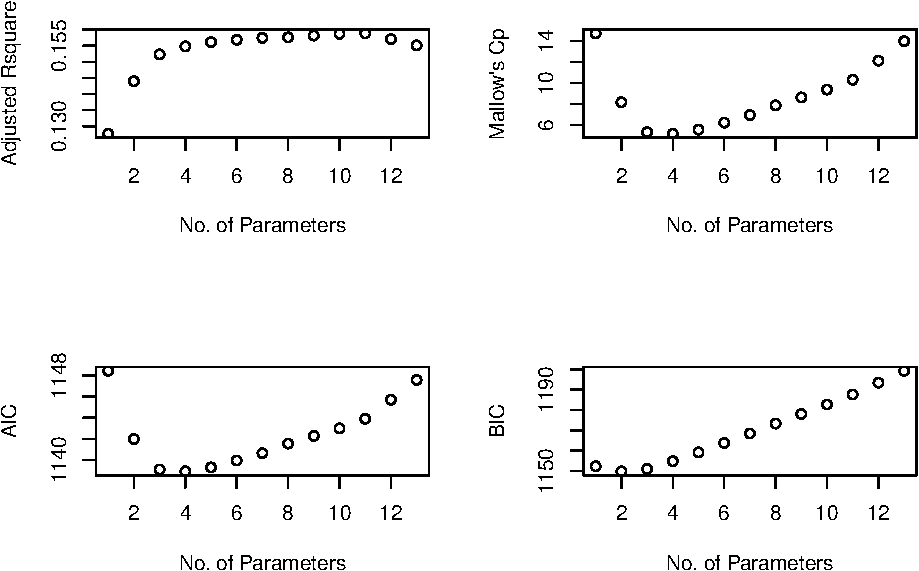
\includegraphics[keepaspectratio]{_main_files/figure-latex/unnamed-chunk-81-1.pdf}}

For this particular data set, AIC and BIC end up selecting different models. \textbf{The model selected by AIC is larger than the one selected by BIC}, which is common. AIC favors larger models while BIC favors smaller models. Although the model selected by BIC does not have the smallest AIC score, its AIC score is very close to the smallest one.

\begin{Shaded}
\begin{Highlighting}[]
\FunctionTok{cbind}\NormalTok{(rs}\SpecialCharTok{$}\NormalTok{which[}\FunctionTok{which.min}\NormalTok{(Aic),], rs}\SpecialCharTok{$}\NormalTok{which[}\FunctionTok{which.min}\NormalTok{(Bic), ])}
\end{Highlighting}
\end{Shaded}

\begin{verbatim}
##              [,1]  [,2]
## (Intercept)  TRUE  TRUE
## age         FALSE FALSE
## Medu         TRUE  TRUE
## Fedu        FALSE FALSE
## traveltime  FALSE FALSE
## studytime   FALSE FALSE
## failures     TRUE  TRUE
## famrel      FALSE FALSE
## freetime     TRUE FALSE
## goout        TRUE FALSE
## Dalc        FALSE FALSE
## Walc        FALSE FALSE
## health      FALSE FALSE
## absences    FALSE FALSE
\end{verbatim}

\texttt{leaps} does not return AIC, but BIC. Its BIC differs from what has been computed above, but the difference is a constant, so the two BIC formulas (ours and the one used by leaps) are essentially the same.

\begin{Shaded}
\begin{Highlighting}[]
\FunctionTok{cbind}\NormalTok{(rs}\SpecialCharTok{$}\NormalTok{bic, Bic, rs}\SpecialCharTok{$}\NormalTok{bic }\SpecialCharTok{{-}}\NormalTok{ Bic)}
\end{Highlighting}
\end{Shaded}

\begin{verbatim}
##                       Bic          
##  [1,] -43.004859 1152.406 -1195.411
##  [2,] -45.475340 1149.936 -1195.411
##  [3,] -44.374670 1151.036 -1195.411
##  [4,] -40.562949 1154.848 -1195.411
##  [5,] -36.222213 1159.189 -1195.411
##  [6,] -31.587827 1163.823 -1195.411
##  [7,] -26.916684 1168.494 -1195.411
##  [8,] -22.029154 1173.382 -1195.411
##  [9,] -17.328400 1178.082 -1195.411
## [10,] -12.638892 1182.772 -1195.411
## [11,]  -7.758187 1187.653 -1195.411
## [12,]  -1.965927 1193.445 -1195.411
## [13,]   3.879571 1199.290 -1195.411
\end{verbatim}

What are the 2nd and 3rd best models in terms of AIC/BIC?
This cannot be answered by looking at the AIC/BIC plots shown above. Instead, we need to run the following code.

\begin{Shaded}
\begin{Highlighting}[]
\NormalTok{regsubsets\_model}\FloatTok{.1} \OtherTok{=} \FunctionTok{regsubsets}\NormalTok{(Grades }\SpecialCharTok{\textasciitilde{}}\NormalTok{ ., }\AttributeTok{data=}\NormalTok{stu\_performance, }\AttributeTok{nbest =} \DecValTok{3}\NormalTok{, }\AttributeTok{nvmax =}\NormalTok{ p)}
\NormalTok{rs}\FloatTok{.1} \OtherTok{=} \FunctionTok{summary}\NormalTok{(regsubsets\_model}\FloatTok{.1}\NormalTok{)}
\CommentTok{\#rs.1$which}
\NormalTok{msize}\FloatTok{.1} \OtherTok{=} \FunctionTok{apply}\NormalTok{(rs}\FloatTok{.1}\SpecialCharTok{$}\NormalTok{which, }\DecValTok{1}\NormalTok{, sum) }\SpecialCharTok{{-}} \DecValTok{1}
\end{Highlighting}
\end{Shaded}

\begin{Shaded}
\begin{Highlighting}[]
\FunctionTok{par}\NormalTok{(}\AttributeTok{mfrow=}\FunctionTok{c}\NormalTok{(}\DecValTok{1}\NormalTok{,}\DecValTok{2}\NormalTok{))}
\NormalTok{Aic}\FloatTok{.1} \OtherTok{=}\NormalTok{ n}\SpecialCharTok{*}\FunctionTok{log}\NormalTok{(rs}\FloatTok{.1}\SpecialCharTok{$}\NormalTok{rss}\SpecialCharTok{/}\NormalTok{n) }\SpecialCharTok{+} \DecValTok{2}\SpecialCharTok{*}\NormalTok{msize}\FloatTok{.1}
\NormalTok{Bic}\FloatTok{.1} \OtherTok{=}\NormalTok{ n}\SpecialCharTok{*}\FunctionTok{log}\NormalTok{(rs}\FloatTok{.1}\SpecialCharTok{$}\NormalTok{rss}\SpecialCharTok{/}\NormalTok{n) }\SpecialCharTok{+}\NormalTok{ msize}\FloatTok{.1}\SpecialCharTok{*}\FunctionTok{log}\NormalTok{(n)}
\FunctionTok{plot}\NormalTok{(msize}\FloatTok{.1}\NormalTok{, Aic}\FloatTok{.1}\NormalTok{, }\AttributeTok{xlab=}\StringTok{"No. of Parameters"}\NormalTok{, }\AttributeTok{ylab =} \StringTok{"AIC"}\NormalTok{)}
\FunctionTok{plot}\NormalTok{(msize}\FloatTok{.1}\NormalTok{, Bic}\FloatTok{.1}\NormalTok{, }\AttributeTok{xlab=}\StringTok{"No. of Parameters"}\NormalTok{, }\AttributeTok{ylab =} \StringTok{"BIC"}\NormalTok{)}
\end{Highlighting}
\end{Shaded}

\pandocbounded{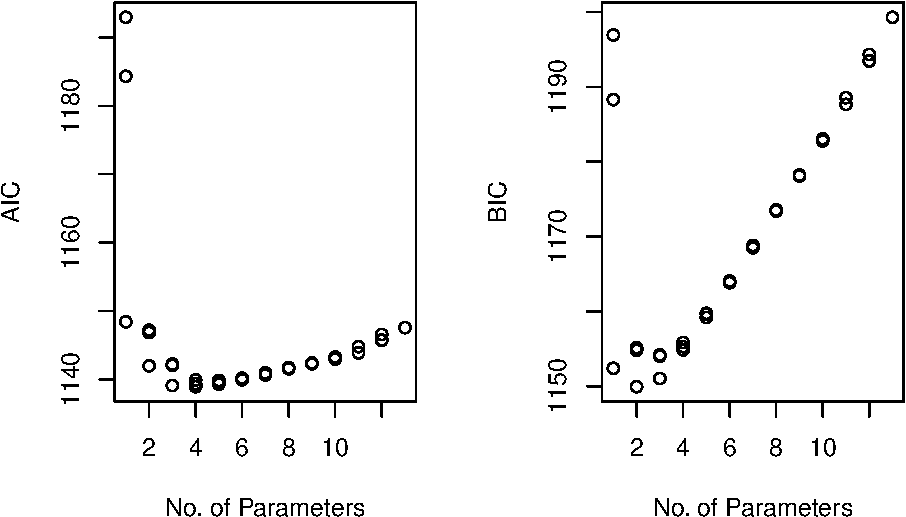
\includegraphics[keepaspectratio]{_main_files/figure-latex/unnamed-chunk-85-1.pdf}}

\begin{Shaded}
\begin{Highlighting}[]
\FunctionTok{par}\NormalTok{(}\AttributeTok{mfrow=}\FunctionTok{c}\NormalTok{(}\DecValTok{1}\NormalTok{,}\DecValTok{2}\NormalTok{))}
\FunctionTok{plot}\NormalTok{(msize}\FloatTok{.1}\NormalTok{, Aic}\FloatTok{.1}\NormalTok{, }\AttributeTok{ylim =} \FunctionTok{c}\NormalTok{(}\DecValTok{1135}\NormalTok{, }\DecValTok{1152}\NormalTok{), }\AttributeTok{xlab=}\StringTok{"No. of Parameters"}\NormalTok{, }\AttributeTok{ylab =} \StringTok{"AIC"}\NormalTok{)}
\FunctionTok{plot}\NormalTok{(msize}\FloatTok{.1}\NormalTok{, Bic}\FloatTok{.1}\NormalTok{, }\AttributeTok{ylim =} \FunctionTok{c}\NormalTok{(}\DecValTok{1140}\NormalTok{, }\DecValTok{1230}\NormalTok{), }\AttributeTok{xlab=}\StringTok{"No. of Parameters"}\NormalTok{, }\AttributeTok{ylab =} \StringTok{"BIC"}\NormalTok{)}
\end{Highlighting}
\end{Shaded}

\pandocbounded{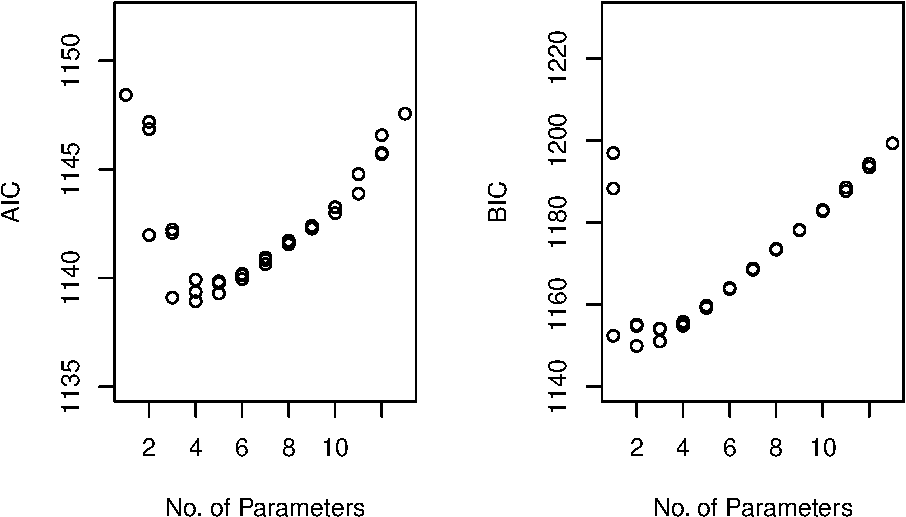
\includegraphics[keepaspectratio]{_main_files/figure-latex/unnamed-chunk-86-1.pdf}}

\begin{Shaded}
\begin{Highlighting}[]
\CommentTok{\# top three models by AIC}
\NormalTok{rs}\FloatTok{.1}\SpecialCharTok{$}\NormalTok{which[}\FunctionTok{order}\NormalTok{(Aic}\FloatTok{.1}\NormalTok{)[}\DecValTok{1}\SpecialCharTok{:}\DecValTok{3}\NormalTok{],]}
\end{Highlighting}
\end{Shaded}

\begin{verbatim}
##   (Intercept)   age Medu  Fedu traveltime studytime failures famrel freetime
## 4        TRUE FALSE TRUE FALSE      FALSE     FALSE     TRUE  FALSE     TRUE
## 3        TRUE FALSE TRUE FALSE      FALSE     FALSE     TRUE  FALSE    FALSE
## 5        TRUE FALSE TRUE FALSE       TRUE     FALSE     TRUE  FALSE     TRUE
##   goout  Dalc  Walc health absences
## 4  TRUE FALSE FALSE  FALSE    FALSE
## 3  TRUE FALSE FALSE  FALSE    FALSE
## 5  TRUE FALSE FALSE  FALSE    FALSE
\end{verbatim}

\begin{Shaded}
\begin{Highlighting}[]
\CommentTok{\# top three models by BIC}
\NormalTok{rs}\FloatTok{.1}\SpecialCharTok{$}\NormalTok{which[}\FunctionTok{order}\NormalTok{(Bic}\FloatTok{.1}\NormalTok{)[}\DecValTok{1}\SpecialCharTok{:}\DecValTok{3}\NormalTok{],]}
\end{Highlighting}
\end{Shaded}

\begin{verbatim}
##   (Intercept)   age  Medu  Fedu traveltime studytime failures famrel freetime
## 2        TRUE FALSE  TRUE FALSE      FALSE     FALSE     TRUE  FALSE    FALSE
## 3        TRUE FALSE  TRUE FALSE      FALSE     FALSE     TRUE  FALSE    FALSE
## 1        TRUE FALSE FALSE FALSE      FALSE     FALSE     TRUE  FALSE    FALSE
##   goout  Dalc  Walc health absences
## 2 FALSE FALSE FALSE  FALSE    FALSE
## 3  TRUE FALSE FALSE  FALSE    FALSE
## 1 FALSE FALSE FALSE  FALSE    FALSE
\end{verbatim}

\subsubsection{\texorpdfstring{Subset Selection via the \texttt{step} fucntion}{Subset Selection via the step fucntion}}\label{subset-selection-via-the-step-fucntion}

We can use the \textbf{stepwise} approach to search possible models moving forward, backwards or in both directions (stepwise).

The \texttt{R} function to do this is the \texttt{step} function. The default is the stepwise method, so if we want to change this, we choose the \texttt{direction} option. The method by default outputs \textbf{all} the steps of the algorithm, so we can set \texttt{trace=0} if we do not want to see the intermediate results. Also, the default criterion for model selection is the \texttt{AIC}. However, we can select the BIC criterion by selecting \texttt{k\ =\ long(n)}.

\begin{Shaded}
\begin{Highlighting}[]
\DocumentationTok{\#\# Stepwise AIC}

\NormalTok{stepAIC }\OtherTok{=} \FunctionTok{step}\NormalTok{(performance.full, }\AttributeTok{trace=}\DecValTok{0}\NormalTok{, }\AttributeTok{direction=}\StringTok{"both"}\NormalTok{)  }
\CommentTok{\#stepAIC = step(performance.full, direction="both")}
\end{Highlighting}
\end{Shaded}

\begin{Shaded}
\begin{Highlighting}[]
\DocumentationTok{\#\# Stepwise BIC}

\NormalTok{n }\OtherTok{=} \FunctionTok{dim}\NormalTok{(stu\_performance)[}\DecValTok{1}\NormalTok{]}
\NormalTok{stepBIC }\OtherTok{=} \FunctionTok{step}\NormalTok{(performance.full, }\AttributeTok{trace=}\DecValTok{0}\NormalTok{, }\AttributeTok{direction=}\StringTok{"both"}\NormalTok{, }\AttributeTok{k=}\FunctionTok{log}\NormalTok{(n))      }
\end{Highlighting}
\end{Shaded}

If we want to retrieve the output from the \texttt{step} function, then we can use the following code:

\begin{Shaded}
\begin{Highlighting}[]
\NormalTok{sel.var.AIC }\OtherTok{=} \FunctionTok{attr}\NormalTok{(stepAIC}\SpecialCharTok{$}\NormalTok{terms, }\StringTok{"term.labels"}\NormalTok{)}
\NormalTok{sel.var.BIC }\OtherTok{=} \FunctionTok{attr}\NormalTok{(stepBIC}\SpecialCharTok{$}\NormalTok{terms, }\StringTok{"term.labels"}\NormalTok{)}
\NormalTok{sel.var.AIC}
\end{Highlighting}
\end{Shaded}

\begin{verbatim}
## [1] "Medu"     "failures" "freetime" "goout"
\end{verbatim}

\begin{Shaded}
\begin{Highlighting}[]
\FunctionTok{length}\NormalTok{(sel.var.AIC)}
\end{Highlighting}
\end{Shaded}

\begin{verbatim}
## [1] 4
\end{verbatim}

\begin{Shaded}
\begin{Highlighting}[]
\FunctionTok{length}\NormalTok{(sel.var.BIC)}
\end{Highlighting}
\end{Shaded}

\begin{verbatim}
## [1] 2
\end{verbatim}

\begin{Shaded}
\begin{Highlighting}[]
\FunctionTok{c}\NormalTok{(}\StringTok{"Medu"}\NormalTok{, }\StringTok{"failures"}\NormalTok{,}\StringTok{"freetime"}\NormalTok{, }\StringTok{"goout"}\NormalTok{) }\SpecialCharTok{\%in\%}\NormalTok{ sel.var.AIC}
\end{Highlighting}
\end{Shaded}

\begin{verbatim}
## [1] TRUE TRUE TRUE TRUE
\end{verbatim}

\begin{Shaded}
\begin{Highlighting}[]
\NormalTok{sel.var.BIC }\SpecialCharTok{\%in\%}\NormalTok{ sel.var.AIC}
\end{Highlighting}
\end{Shaded}

\begin{verbatim}
## [1] TRUE TRUE
\end{verbatim}

\subsubsection{LASSO and RIDGE Regression}\label{lasso-and-ridge-regression}

\texttt{glmnet} is the library needed for both lasso (\(\alpha=1\)) and ridge (\(\alpha=0\)). Check more \texttt{glmnet} examples at \url{https://web.stanford.edu/~hastie/glmnet/glmnet_beta.html}

\begin{Shaded}
\begin{Highlighting}[]
\FunctionTok{library}\NormalTok{(glmnet)}
\end{Highlighting}
\end{Shaded}

\begin{verbatim}
## Loading required package: Matrix
\end{verbatim}

\begin{verbatim}
## Loaded glmnet 4.1-10
\end{verbatim}

\begin{Shaded}
\begin{Highlighting}[]
\DocumentationTok{\#\# The input in the glmnet function should be in matrix format:}

\NormalTok{X }\OtherTok{=} \FunctionTok{as.matrix}\NormalTok{(stu\_performance[, }\FunctionTok{names}\NormalTok{(stu\_performance) }\SpecialCharTok{!=} \StringTok{"Grades"}\NormalTok{])}
\NormalTok{Y }\OtherTok{=}\NormalTok{ stu\_performance}\SpecialCharTok{$}\NormalTok{Grades}
\end{Highlighting}
\end{Shaded}

We are going to split the data in training (80\%) and testing (20\%) data sets. Then, we will select the variables in the training set and estimate the coefficients and compute the average MSE on the testing data.

\begin{Shaded}
\begin{Highlighting}[]
\DocumentationTok{\#\# Training/ Testing Data Sets}

\NormalTok{ntest }\OtherTok{=} \FunctionTok{round}\NormalTok{(n}\SpecialCharTok{*}\FloatTok{0.2}\NormalTok{);    }\DocumentationTok{\#\# testing set sample size}
\NormalTok{ntrain }\OtherTok{=}\NormalTok{ n }\SpecialCharTok{{-}}\NormalTok{ ntest;      }\DocumentationTok{\#\# training set sample size}
\NormalTok{test.id }\OtherTok{=} \FunctionTok{sample}\NormalTok{(}\DecValTok{1}\SpecialCharTok{:}\NormalTok{n, ntest);   }\DocumentationTok{\#\# sampling indices for the test data}

\NormalTok{Ytest }\OtherTok{=}\NormalTok{ Y[test.id]; }\DocumentationTok{\#\# Response in the Testing data}
\end{Highlighting}
\end{Shaded}

Training the \textbf{full model} in the \emph{training} data set:

\begin{Shaded}
\begin{Highlighting}[]
\DocumentationTok{\#\# Fit the Full model in the training data}
\NormalTok{full.model }\OtherTok{=} \FunctionTok{lm}\NormalTok{(Y[}\SpecialCharTok{{-}}\NormalTok{test.id]}\SpecialCharTok{\textasciitilde{}}\NormalTok{., }\AttributeTok{data =}\NormalTok{ stu\_performance[}\SpecialCharTok{{-}}\NormalTok{test.id, ])}
\end{Highlighting}
\end{Shaded}

We then use the full model to \textbf{predict} values and \emph{compute the MSE on the testing data set}:

\begin{Shaded}
\begin{Highlighting}[]
\DocumentationTok{\#\# Predicted values on the testing data set}
\NormalTok{Ytest.pred }\OtherTok{=} \FunctionTok{predict}\NormalTok{(full.model, }\AttributeTok{newdata=}\NormalTok{ stu\_performance[test.id, ]);}

\DocumentationTok{\#\# Averaged MSE on the test set}
\FunctionTok{sum}\NormalTok{((Ytest }\SpecialCharTok{{-}}\NormalTok{ Ytest.pred)}\SpecialCharTok{\^{}}\DecValTok{2}\NormalTok{)}\SpecialCharTok{/}\NormalTok{ntest }
\end{Highlighting}
\end{Shaded}

\begin{verbatim}
## [1] 1.630006e-29
\end{verbatim}

\chapter{NonLinear Regression}\label{nonlinear-regression}

As we discussed in the previous sections, a Multiple Linear Regression model has a set of assumptions on the error terms (normality, homoscedasticity, independence) as well as limitations, such as the linearity assumption.

If one or more of these assumptions are not satisfied, then the applicability of our model is restricted. In this section, we will introduce models that lift the linearity assumption. Therefore, we are going to discuss the \emph{three} most popular \emph{nonlinear} regression models:

\begin{enumerate}
\def\labelenumi{(\roman{enumi})}
\tightlist
\item
  Polynomial Regression
\item
  Splines Regression
\item
  Smoothing Splines
\end{enumerate}

\subsection{A Note on Nonlinearity}\label{a-note-on-nonlinearity}

Assume that the true underlying model is of the following form:
\[Y = f(\mathbf{X}) + \varepsilon\]
where \(\varepsilon\) satisfies the usual assumptions. So far we have been \textbf{approximating} the unknown function \(f\) via a multiple linear regression model:
\[Y_i = \beta_0 + \beta_1 X_{i1} +  \beta_2 X_{i2} +\ldots +  \beta_p X_{ip} +\varepsilon_i \]
The MLR model above is \textbf{linear} \textbf{both} with respect to the predictors (\(X_{ij}\)) \textbf{and} with respect to the coefficients (\(\beta_j\)).

Consider now the following models:
\[Y_i = \beta_1 X_{i1} +  \beta_2 X_{i1}^2 +\beta_3 X_{i2} + \beta_4 X_{i2}^2 +  \beta_5 X_{i1} X_{i2} +\varepsilon_i \]
or
\[\log_{10}Y_i = \beta_1 X_{i1} +  \beta_2 \sqrt{X_{i1}} +\beta_3 e^{X_{i3}} +\varepsilon_i\]
These two models are both \emph{non-linear} with respect to the predictors but \textbf{linear} with respect to the coefficients \(\beta_j\).

On the other side, the model below
\[Y_i =  \frac{\gamma_0}{1+ \gamma_1 e^{\gamma_2 X_i}} + \varepsilon_i \]
is non-linear both with respect to the parameters \emph{and} the predictors.

During the course of this week, we are going to approximate the general nonlinear model, using nonlinear models with respect to the predictors (so that we describe the underlying nonlinear relationship between response and features), but all the models that we will introduce with be \emph{linear with respect to the coefficients/parameters}. In this way, one can think of the models we will work with as models in which the features have been transformed to a new predictor in a nonlinear fashion.

The main advantage of this approach is that we manage to describe (quite efficientily most of the time) a nonlinear relationship between predictor and features, but at the same time we are able to estimate the model parameters easily.

To be more specific, the coefficients will still be obtained via a least-squares approach which (due to the linearity wrt predictor assumption) will result in a system of linear equations as before.

\section{Polynomial Regression}\label{polynomial-regression}

The simplest form of nonlinear regression is the polynomial regression which is an extension of the linear model by adding higher order terms of the predictor(s). To study this type of regression, we need to first define the polynomial basis functions.

\subsection{Polynomial Basis Functions}\label{polynomial-basis-functions}

If \(b_j(x)\) is the \(j\)th basis function, then \(f\) has the following representation
\[f(x) = \sum_{j=0}^{d} b_j(x) \beta_j\]
for some values \(\beta_j\). Therefore, we can write the nonlinear model \(y_i = f(x_i) + \varepsilon_i\) as a linear model (with respect to the coefficients)
\[y_i = \beta_0 + \sum_{j=1}^{d} b_j(x_i) \beta_j + \varepsilon_i\]
Suppose that \(f\) is believed to be a 4th order polynomial, so \emph{the space of polynomials of order 4 and below contains \(f\)}.

A basis for this space is
\begin{align*}
b_0(x) &= 1\\
b_1(x) &= x\\
b_2(x) &= x^2\\
b_3(x) &= x^3\\
b_4(x) &= x^4
\end{align*}
so that the model becomes
\[y_i = \underbrace{\beta_0 + \beta_1 x_i+\beta_2 x^2_i+ \beta_3 x^3_i + \beta_4 x^4_i}_{= \beta_0 + \sum_{j=1}^{d} b_j(x_i) \beta_j} +\varepsilon_i\]

\textbf{Illustration of the Polynomial Basis Functions}

Representation of a function in terms of basis functions using a polynomial basis. The following code creates the plots the polynomial basis function up to order 4

\begin{Shaded}
\begin{Highlighting}[]
\NormalTok{x}\OtherTok{=}\FunctionTok{seq}\NormalTok{(}\DecValTok{0}\NormalTok{, }\DecValTok{1}\NormalTok{, }\AttributeTok{by=}\FloatTok{0.001}\NormalTok{)}
\NormalTok{b0 }\OtherTok{=} \FunctionTok{rep}\NormalTok{(}\DecValTok{1}\NormalTok{, }\FunctionTok{length}\NormalTok{(x))}
\NormalTok{b1 }\OtherTok{=}\NormalTok{ x}
\NormalTok{b2 }\OtherTok{=}\NormalTok{ x}\SpecialCharTok{\^{}}\DecValTok{2}
\NormalTok{b3 }\OtherTok{=}\NormalTok{ x}\SpecialCharTok{\^{}}\DecValTok{3}
\NormalTok{b4 }\OtherTok{=}\NormalTok{ x}\SpecialCharTok{\^{}}\DecValTok{4}

\NormalTok{fun1 }\OtherTok{=} \DecValTok{4}\SpecialCharTok{*}\NormalTok{b0 }\SpecialCharTok{{-}}\DecValTok{10}\SpecialCharTok{*}\NormalTok{ b1 }\SpecialCharTok{+} \DecValTok{16}\SpecialCharTok{*}\NormalTok{b2 }\SpecialCharTok{+} \DecValTok{2}\SpecialCharTok{*}\NormalTok{b3 }\SpecialCharTok{{-}}\DecValTok{10}\SpecialCharTok{*}\NormalTok{b4}

\FunctionTok{par}\NormalTok{(}\AttributeTok{mfrow =} \FunctionTok{c}\NormalTok{(}\DecValTok{2}\NormalTok{,}\DecValTok{3}\NormalTok{))}
\FunctionTok{plot}\NormalTok{(x, b0, }\AttributeTok{type=}\StringTok{\textquotesingle{}l\textquotesingle{}}\NormalTok{, }\AttributeTok{lty=}\DecValTok{3}\NormalTok{, }\AttributeTok{ylab=}\FunctionTok{expression}\NormalTok{(}\StringTok{"b"}\NormalTok{[}\DecValTok{0}\NormalTok{]}\SpecialCharTok{*}\StringTok{"(x)=1"}\NormalTok{))}
\FunctionTok{plot}\NormalTok{(x, b1, }\AttributeTok{type=}\StringTok{\textquotesingle{}l\textquotesingle{}}\NormalTok{,}\AttributeTok{lty=}\DecValTok{3}\NormalTok{, }\AttributeTok{ylab=}\FunctionTok{expression}\NormalTok{(}\StringTok{"b"}\NormalTok{[}\DecValTok{1}\NormalTok{]}\SpecialCharTok{*}\StringTok{"(x)=x"}\NormalTok{))}
\FunctionTok{plot}\NormalTok{(x, b2, }\AttributeTok{type=}\StringTok{\textquotesingle{}l\textquotesingle{}}\NormalTok{,}\AttributeTok{lty=}\DecValTok{3}\NormalTok{, }\AttributeTok{ylab=}\FunctionTok{expression}\NormalTok{(}\StringTok{"b"}\NormalTok{[}\DecValTok{2}\NormalTok{]}\SpecialCharTok{*}\StringTok{"(x)=x"}\SpecialCharTok{\^{}}\DecValTok{2}\NormalTok{))}
\FunctionTok{plot}\NormalTok{(x, b3, }\AttributeTok{type=}\StringTok{\textquotesingle{}l\textquotesingle{}}\NormalTok{,}\AttributeTok{lty=}\DecValTok{3}\NormalTok{, }\AttributeTok{ylab=}\FunctionTok{expression}\NormalTok{(}\StringTok{"b"}\NormalTok{[}\DecValTok{3}\NormalTok{]}\SpecialCharTok{*}\StringTok{"(x)=x"}\SpecialCharTok{\^{}}\DecValTok{3}\NormalTok{))}
\FunctionTok{plot}\NormalTok{(x, b4, }\AttributeTok{type=}\StringTok{\textquotesingle{}l\textquotesingle{}}\NormalTok{,}\AttributeTok{lty=}\DecValTok{3}\NormalTok{, }\AttributeTok{ylab=}\FunctionTok{expression}\NormalTok{(}\StringTok{"b"}\NormalTok{[}\DecValTok{4}\NormalTok{]}\SpecialCharTok{*}\StringTok{"(x)=x"}\SpecialCharTok{\^{}}\DecValTok{4}\NormalTok{))}
\FunctionTok{plot}\NormalTok{(x, fun1, }\AttributeTok{type=}\StringTok{\textquotesingle{}l\textquotesingle{}}\NormalTok{, }\AttributeTok{ylab=}\StringTok{"f(x)"}\NormalTok{, }\AttributeTok{main=}\FunctionTok{expression}\NormalTok{(}\StringTok{"f(x) =  4 {-} 10 x + 16 x"}\SpecialCharTok{\^{}}\DecValTok{2}\SpecialCharTok{*}\StringTok{"+ 2 x"}\SpecialCharTok{\^{}}\DecValTok{3}\SpecialCharTok{*}\StringTok{"{-} 10 x"}\SpecialCharTok{\^{}}\DecValTok{4}\NormalTok{), }\AttributeTok{col=}\StringTok{"blue"}\NormalTok{, }\AttributeTok{lwd=}\DecValTok{2}\NormalTok{)}
\end{Highlighting}
\end{Shaded}

\pandocbounded{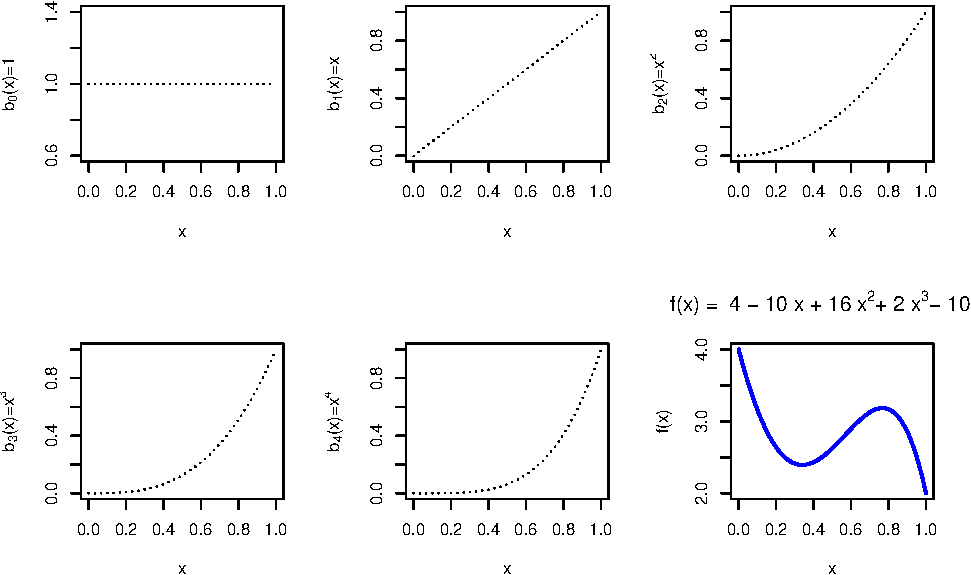
\includegraphics[keepaspectratio]{_main_files/figure-latex/unnamed-chunk-96-1.pdf}}

\subsection{Polynomial Regression}\label{polynomial-regression-1}

From now on, assume \(x \in \mathbb{R}\) is one-dimensional, and extensions to multi-dimensional cases will be discussed later. So, for \(x_i \in \mathbb{R}\),
\[
y_i = \beta_0 + \beta_1 x_i + \beta_2 x_i^2 + \cdots + \beta_d x_i^d + \varepsilon_i
\]

Then, we create the new variables \(X_2 = X^2, \ldots, X_d = X^d\), and treat this as a multiple linear regression model:
\[
\begin{pmatrix}
y_1 \\ y_2 \\ \vdots \\ y_n
\end{pmatrix}_{n \times 1}
=
\begin{pmatrix}
1 & x_1 & x_1^2 & \cdots & x_1^d \\
1 & x_2 & x_2^2 & \cdots & x_2^d \\
\vdots & \vdots & \vdots & \ddots & \vdots \\
1 & x_n & x_n^2 & \cdots & x_n^d
\end{pmatrix}_{n \times (d+1)}
\begin{pmatrix}
\beta_0 \\ \beta_1 \\ \vdots \\ \beta_d
\end{pmatrix}_{(d+1) \times 1}
+ \varepsilon
\]

Therefore, we can say that a polynomial regression model is defined as follows:

\textbf{Polynomial Regression Model}

A \emph{non-linear} model can be represented using a basis of polynomial functions as follows:
\[y_i = f(x_i) + \varepsilon_i \,\,\, \longrightarrow \,\,\, y_i =\beta_0 + \sum_{j=1}^{d} b_j(x_i) \beta_j + \varepsilon_i\]
where \(d\) is the degree of the polynomial component.

\subsubsection*{\texorpdfstring{How do we choose \(d\)? }{How do we choose d? }}\label{how-do-we-choose-d}
\addcontentsline{toc}{subsubsection}{How do we choose \(d\)? }

\begin{enumerate}
\def\labelenumi{\arabic{enumi}.}
\item
  \emph{Forward Approach}: Keep \emph{adding} terms until the \emph{last} added term is not significant.
\item
  \emph{Backward Approach}: Start with a large \(d\), and keep \emph{eliminating} the terms that are not statistically significant, starting with the highest order term.
\end{enumerate}

Once we pick a value of \(d\), then we usually do \textbf{not} test the significance of the lower-order terms. Therefore, when we decide to use a polynomial of degree \(d\), by default, we include \emph{all the lower-order terms in our model}.

Reasoning
In regression analysis, we do not want our results to be affected by a change of location/scale of the data. Consider the following example:
Suppose the data \(\{y_i,x_i\}_{i=1}^n\) are generated by the model:
\[y_i=x_i^2 + \varepsilon_i,\quad \varepsilon_i \sim \mathcal{N}(0,\sigma^2)\]
But, they are instead recorded as \(\{z_i,x_i\}_{i=1}^n\), where \(z_i=x_i+2\), that is,
\[y_i=(z_i-2)^2 + \varepsilon_i=4 -4z_i +z_i^2+\varepsilon_i\]
The linear term could become significant, if we shift the \(x\) values.

\textbf{Exception}: When we have a particular polynomial function in mind, e.g.~the data are collected to test a particular physics formula \(Y\approx X^2 + constant\), then you should test whether you can drop the linear term.

\textbf{The Chicago Pumpkins Example}

The \texttt{pumpkins.csv} data set contains information regarding the \texttt{size} and \texttt{price} of pumpkins sold in the Chicago area (data can be found here.). Our goal in this example is to \emph{predict} the \texttt{size\ of\ the\ pumpkin} (response) based on its \texttt{price} (predictor).

The scatter plot of the data is shown below:

\begin{Shaded}
\begin{Highlighting}[]
\NormalTok{pumpkins }\OtherTok{=} \FunctionTok{read.csv}\NormalTok{(}\StringTok{"data/week4/chicagopumpkins.csv"}\NormalTok{,}\AttributeTok{header=}\ConstantTok{TRUE}\NormalTok{)}
\FunctionTok{plot}\NormalTok{(pumpkins}\SpecialCharTok{$}\NormalTok{price, pumpkins}\SpecialCharTok{$}\NormalTok{size, }\AttributeTok{pch=}\DecValTok{20}\NormalTok{, }\AttributeTok{xlab=}\StringTok{"Pumpkin\textquotesingle{}s Price"}\NormalTok{, }\AttributeTok{ylab=}\StringTok{"Pumpkins\textquotesingle{} Size"}\NormalTok{)}
\end{Highlighting}
\end{Shaded}

\pandocbounded{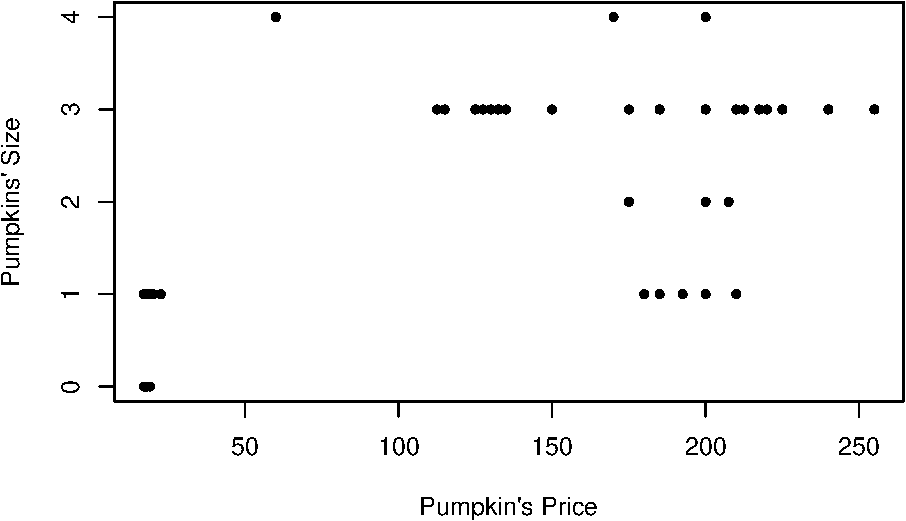
\includegraphics[keepaspectratio]{_main_files/figure-latex/unnamed-chunk-97-1.pdf}}
We see that a linear fit is probably \emph{not} a good idea. Indeed,

\begin{Shaded}
\begin{Highlighting}[]
\NormalTok{lm.pumpkins }\OtherTok{=} \FunctionTok{lm}\NormalTok{(size }\SpecialCharTok{\textasciitilde{}}\NormalTok{ price, }\AttributeTok{data=}\NormalTok{pumpkins)}
\FunctionTok{summary}\NormalTok{(lm.pumpkins)}
\end{Highlighting}
\end{Shaded}

\begin{verbatim}
## 
## Call:
## lm(formula = size ~ price, data = pumpkins)
## 
## Residuals:
##     Min      1Q  Median      3Q     Max 
## -1.6272 -0.7594  0.2244  0.3728  2.8245 
## 
## Coefficients:
##              Estimate Std. Error t value Pr(>|t|)    
## (Intercept) 0.5948315  0.0988339   6.018 6.35e-09 ***
## price       0.0096781  0.0006856  14.117  < 2e-16 ***
## ---
## Signif. codes:  0 '***' 0.001 '**' 0.01 '*' 0.05 '.' 0.1 ' ' 1
## 
## Residual standard error: 0.9477 on 246 degrees of freedom
## Multiple R-squared:  0.4475, Adjusted R-squared:  0.4453 
## F-statistic: 199.3 on 1 and 246 DF,  p-value: < 2.2e-16
\end{verbatim}

Although the predictor is significant at explaining the response, the \(R^2\) is on the lower end and the scatter plot does not support a straight line as a good fit.

\begin{Shaded}
\begin{Highlighting}[]
\FunctionTok{plot}\NormalTok{(size }\SpecialCharTok{\textasciitilde{}}\NormalTok{ price, }\AttributeTok{data=}\NormalTok{pumpkins)}
\FunctionTok{points}\NormalTok{(size }\SpecialCharTok{\textasciitilde{}}\NormalTok{ price, }\AttributeTok{data=}\NormalTok{pumpkins, }\AttributeTok{pch=}\DecValTok{8}\NormalTok{)}
\FunctionTok{abline}\NormalTok{(lm.pumpkins, }\AttributeTok{col=}\StringTok{"blue"}\NormalTok{, }\AttributeTok{lwd=}\DecValTok{2}\NormalTok{)}
\end{Highlighting}
\end{Shaded}

\pandocbounded{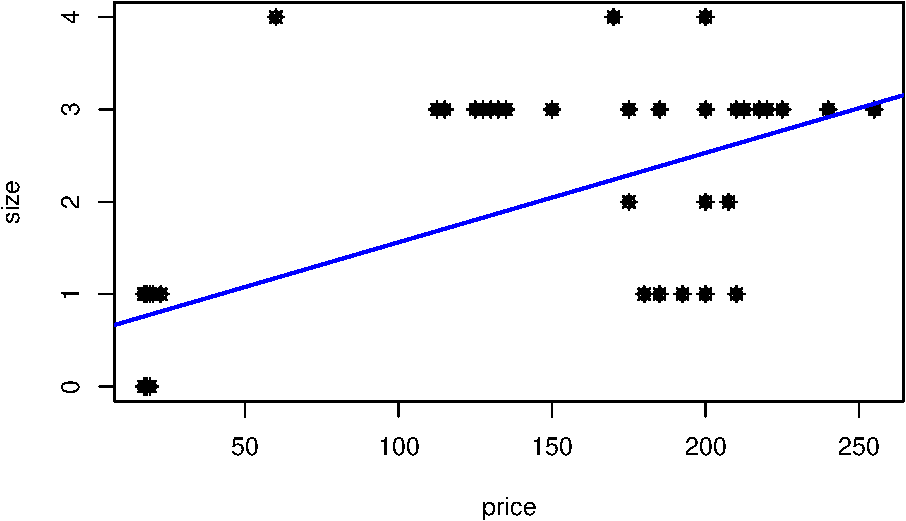
\includegraphics[keepaspectratio]{_main_files/figure-latex/unnamed-chunk-99-1.pdf}}

We want to select a \emph{higher order} model and we will do so following a Forward Selection approach first and a Backward Selection method second:

\begin{enumerate}
\def\labelenumi{(\arabic{enumi})}
\tightlist
\item
  We start with a Forward Selection approach, i.e.~we start by a linear model, and we keep \textbf{adding} higher order terms until the added term becomes \emph{statistically insignificant}.
\end{enumerate}

\begin{Shaded}
\begin{Highlighting}[]
\CommentTok{\# Forward Selection}
\NormalTok{lm.pumpkins }\OtherTok{=}  \FunctionTok{lm}\NormalTok{(size }\SpecialCharTok{\textasciitilde{}}\NormalTok{ price , }\AttributeTok{data=}\NormalTok{pumpkins)}
\FunctionTok{summary}\NormalTok{(lm.pumpkins)}
\end{Highlighting}
\end{Shaded}

\begin{verbatim}
## 
## Call:
## lm(formula = size ~ price, data = pumpkins)
## 
## Residuals:
##     Min      1Q  Median      3Q     Max 
## -1.6272 -0.7594  0.2244  0.3728  2.8245 
## 
## Coefficients:
##              Estimate Std. Error t value Pr(>|t|)    
## (Intercept) 0.5948315  0.0988339   6.018 6.35e-09 ***
## price       0.0096781  0.0006856  14.117  < 2e-16 ***
## ---
## Signif. codes:  0 '***' 0.001 '**' 0.01 '*' 0.05 '.' 0.1 ' ' 1
## 
## Residual standard error: 0.9477 on 246 degrees of freedom
## Multiple R-squared:  0.4475, Adjusted R-squared:  0.4453 
## F-statistic: 199.3 on 1 and 246 DF,  p-value: < 2.2e-16
\end{verbatim}

\begin{Shaded}
\begin{Highlighting}[]
\NormalTok{lm.pumpkins2 }\OtherTok{=}  \FunctionTok{lm}\NormalTok{(size }\SpecialCharTok{\textasciitilde{}}\NormalTok{ price }\SpecialCharTok{+} \FunctionTok{I}\NormalTok{(price}\SpecialCharTok{\^{}}\DecValTok{2}\NormalTok{), }\AttributeTok{data=}\NormalTok{pumpkins)}
\FunctionTok{summary}\NormalTok{(lm.pumpkins2)}
\end{Highlighting}
\end{Shaded}

\begin{verbatim}
## 
## Call:
## lm(formula = size ~ price + I(price^2), data = pumpkins)
## 
## Residuals:
##     Min      1Q  Median      3Q     Max 
## -1.6438 -0.6029  0.3695  0.4895  2.3941 
## 
## Coefficients:
##               Estimate Std. Error t value Pr(>|t|)    
## (Intercept)  1.093e-01  1.174e-01   0.932    0.353    
## price        3.037e-02  3.208e-03   9.469  < 2e-16 ***
## I(price^2)  -9.051e-05  1.375e-05  -6.582  2.8e-10 ***
## ---
## Signif. codes:  0 '***' 0.001 '**' 0.01 '*' 0.05 '.' 0.1 ' ' 1
## 
## Residual standard error: 0.8754 on 245 degrees of freedom
## Multiple R-squared:  0.5305, Adjusted R-squared:  0.5267 
## F-statistic: 138.4 on 2 and 245 DF,  p-value: < 2.2e-16
\end{verbatim}

\begin{Shaded}
\begin{Highlighting}[]
\NormalTok{lm.pumpkins3 }\OtherTok{=}  \FunctionTok{lm}\NormalTok{(size }\SpecialCharTok{\textasciitilde{}}\NormalTok{ price }\SpecialCharTok{+} \FunctionTok{I}\NormalTok{(price}\SpecialCharTok{\^{}}\DecValTok{2}\NormalTok{) }\SpecialCharTok{+} \FunctionTok{I}\NormalTok{(price}\SpecialCharTok{\^{}}\DecValTok{3}\NormalTok{), }\AttributeTok{data=}\NormalTok{pumpkins)}
\FunctionTok{summary}\NormalTok{(lm.pumpkins3)}
\end{Highlighting}
\end{Shaded}

\begin{verbatim}
## 
## Call:
## lm(formula = size ~ price + I(price^2) + I(price^3), data = pumpkins)
## 
## Residuals:
##     Min      1Q  Median      3Q     Max 
## -1.2786 -0.4937 -0.1368  0.5531  1.8633 
## 
## Coefficients:
##               Estimate Std. Error t value Pr(>|t|)    
## (Intercept) -1.414e+00  1.691e-01   -8.36 4.83e-15 ***
## price        1.256e-01  9.079e-03   13.83  < 2e-16 ***
## I(price^2)  -9.845e-04  8.239e-05  -11.95  < 2e-16 ***
## I(price^3)   2.228e-06  2.034e-07   10.95  < 2e-16 ***
## ---
## Signif. codes:  0 '***' 0.001 '**' 0.01 '*' 0.05 '.' 0.1 ' ' 1
## 
## Residual standard error: 0.7182 on 244 degrees of freedom
## Multiple R-squared:  0.6853, Adjusted R-squared:  0.6814 
## F-statistic: 177.1 on 3 and 244 DF,  p-value: < 2.2e-16
\end{verbatim}

\begin{Shaded}
\begin{Highlighting}[]
\NormalTok{lm.pumpkins4 }\OtherTok{=}  \FunctionTok{lm}\NormalTok{(size }\SpecialCharTok{\textasciitilde{}}\NormalTok{ price }\SpecialCharTok{+} \FunctionTok{I}\NormalTok{(price}\SpecialCharTok{\^{}}\DecValTok{2}\NormalTok{) }\SpecialCharTok{+} \FunctionTok{I}\NormalTok{(price}\SpecialCharTok{\^{}}\DecValTok{3}\NormalTok{) }\SpecialCharTok{+} \FunctionTok{I}\NormalTok{(price}\SpecialCharTok{\^{}}\DecValTok{4}\NormalTok{), }\AttributeTok{data=}\NormalTok{pumpkins)}
\FunctionTok{summary}\NormalTok{(lm.pumpkins4)}
\end{Highlighting}
\end{Shaded}

\begin{verbatim}
## 
## Call:
## lm(formula = size ~ price + I(price^2) + I(price^3) + I(price^4), 
##     data = pumpkins)
## 
## Residuals:
##     Min      1Q  Median      3Q     Max 
## -1.3200 -0.4497 -0.1241  0.5539  1.7925 
## 
## Coefficients:
##               Estimate Std. Error t value Pr(>|t|)    
## (Intercept) -2.871e+00  3.782e-01  -7.590 6.83e-13 ***
## price        2.314e-01  2.630e-02   8.800 2.60e-16 ***
## I(price^2)  -2.565e-03  3.785e-04  -6.776 9.25e-11 ***
## I(price^3)   1.061e-05  1.973e-06   5.378 1.76e-07 ***
## I(price^4)  -1.470e-08  3.443e-09  -4.271 2.80e-05 ***
## ---
## Signif. codes:  0 '***' 0.001 '**' 0.01 '*' 0.05 '.' 0.1 ' ' 1
## 
## Residual standard error: 0.6941 on 243 degrees of freedom
## Multiple R-squared:  0.7073, Adjusted R-squared:  0.7025 
## F-statistic: 146.8 on 4 and 243 DF,  p-value: < 2.2e-16
\end{verbatim}

\begin{Shaded}
\begin{Highlighting}[]
\NormalTok{lm.pumpkins5 }\OtherTok{=}  \FunctionTok{lm}\NormalTok{(size }\SpecialCharTok{\textasciitilde{}}\NormalTok{ price }\SpecialCharTok{+} \FunctionTok{I}\NormalTok{(price}\SpecialCharTok{\^{}}\DecValTok{2}\NormalTok{) }\SpecialCharTok{+} \FunctionTok{I}\NormalTok{(price}\SpecialCharTok{\^{}}\DecValTok{3}\NormalTok{) }\SpecialCharTok{+} \FunctionTok{I}\NormalTok{(price}\SpecialCharTok{\^{}}\DecValTok{4}\NormalTok{)}\SpecialCharTok{+} \FunctionTok{I}\NormalTok{(price}\SpecialCharTok{\^{}}\DecValTok{5}\NormalTok{), }\AttributeTok{data=}\NormalTok{pumpkins)}
\FunctionTok{summary}\NormalTok{(lm.pumpkins5)}
\end{Highlighting}
\end{Shaded}

\begin{verbatim}
## 
## Call:
## lm(formula = size ~ price + I(price^2) + I(price^3) + I(price^4) + 
##     I(price^5), data = pumpkins)
## 
## Residuals:
##      Min       1Q   Median       3Q      Max 
## -1.38082 -0.46537 -0.08211  0.53463  1.91954 
## 
## Coefficients:
##               Estimate Std. Error t value Pr(>|t|)  
## (Intercept) -1.691e+00  7.112e-01  -2.378   0.0182 *
## price        1.305e-01  5.791e-02   2.253   0.0251 *
## I(price^2)  -2.479e-04  1.244e-03  -0.199   0.8422  
## I(price^3)  -1.078e-05  1.113e-05  -0.969   0.3333  
## I(price^4)   7.118e-08  4.409e-08   1.615   0.1077  
## I(price^5)  -1.248e-10  6.386e-11  -1.954   0.0519 .
## ---
## Signif. codes:  0 '***' 0.001 '**' 0.01 '*' 0.05 '.' 0.1 ' ' 1
## 
## Residual standard error: 0.6901 on 242 degrees of freedom
## Multiple R-squared:  0.7118, Adjusted R-squared:  0.7059 
## F-statistic: 119.6 on 5 and 242 DF,  p-value: < 2.2e-16
\end{verbatim}

We see that the \emph{5th order model} has a 5th order term with \emph{\(p\)-value equal to 0.0519}, which is \textbf{higher than 5\%}, so we conclude that the optimal order for the polynomial, according to the forward selection method is \(d=4\). So, the fitted model is:
\[\hat{y}_i = \hat{\beta}_0 + \hat{\beta}_1 x + \hat{\beta}_2 x^2 + \hat{\beta}_3 x^4 + \hat{\beta}_4 x^4 \]

If we plot all the fitted models, we have:

\begin{Shaded}
\begin{Highlighting}[]
\NormalTok{newprice }\OtherTok{=} \FunctionTok{data.frame}\NormalTok{(}\AttributeTok{price=}\FunctionTok{seq}\NormalTok{(}\DecValTok{17}\NormalTok{, }\DecValTok{255}\NormalTok{, }\DecValTok{1}\NormalTok{))}
\FunctionTok{plot}\NormalTok{(pumpkins}\SpecialCharTok{$}\NormalTok{price, pumpkins}\SpecialCharTok{$}\NormalTok{size, }\AttributeTok{pch=}\DecValTok{20}\NormalTok{, }\AttributeTok{ylim=}\FunctionTok{c}\NormalTok{(}\DecValTok{0}\NormalTok{,}\DecValTok{5}\NormalTok{), }\AttributeTok{xlab=}\StringTok{"Pumpkin\textquotesingle{}s Price"}\NormalTok{, }\AttributeTok{ylab=}\StringTok{"Pumpkins\textquotesingle{} Size"}\NormalTok{, }\AttributeTok{main=}\StringTok{"Forward Selection Models"}\NormalTok{)}
\FunctionTok{lines}\NormalTok{(newprice}\SpecialCharTok{$}\NormalTok{price, }\FunctionTok{predict}\NormalTok{(lm.pumpkins, newprice), }\AttributeTok{col=}\StringTok{"yellow"}\NormalTok{, }\AttributeTok{lty=}\DecValTok{1}\NormalTok{, }\AttributeTok{lwd=}\DecValTok{2}\NormalTok{);}
\FunctionTok{lines}\NormalTok{(newprice}\SpecialCharTok{$}\NormalTok{price, }\FunctionTok{predict}\NormalTok{(lm.pumpkins2, newprice), }\AttributeTok{col=}\StringTok{"blue"}\NormalTok{, }\AttributeTok{lty=}\DecValTok{1}\NormalTok{, }\AttributeTok{lwd=}\DecValTok{2}\NormalTok{);}
\FunctionTok{lines}\NormalTok{(newprice}\SpecialCharTok{$}\NormalTok{price, }\FunctionTok{predict}\NormalTok{(lm.pumpkins3, newprice), }\AttributeTok{col=}\StringTok{"orange"}\NormalTok{, }\AttributeTok{lty=}\DecValTok{1}\NormalTok{, }\AttributeTok{lwd=}\DecValTok{2}\NormalTok{);}
\FunctionTok{lines}\NormalTok{(newprice}\SpecialCharTok{$}\NormalTok{price, }\FunctionTok{predict}\NormalTok{(lm.pumpkins4, newprice), }\AttributeTok{col=}\StringTok{"magenta"}\NormalTok{, }\AttributeTok{lty=}\DecValTok{1}\NormalTok{, }\AttributeTok{lwd=}\DecValTok{2}\NormalTok{);}
\FunctionTok{lines}\NormalTok{(newprice}\SpecialCharTok{$}\NormalTok{price, }\FunctionTok{predict}\NormalTok{(lm.pumpkins5, newprice), }\AttributeTok{col=}\StringTok{"green"}\NormalTok{, }\AttributeTok{lty=}\DecValTok{1}\NormalTok{, }\AttributeTok{lwd=}\DecValTok{2}\NormalTok{);}
\FunctionTok{legend}\NormalTok{(}\DecValTok{230}\NormalTok{, }\FloatTok{1.45}\NormalTok{, }\AttributeTok{legend=}\FunctionTok{c}\NormalTok{(}\StringTok{"d=1"}\NormalTok{, }\StringTok{"d=2"}\NormalTok{, }\StringTok{"d=3"}\NormalTok{, }\StringTok{"d=4"}\NormalTok{, }\StringTok{"d=5"}\NormalTok{),}
       \AttributeTok{col=}\FunctionTok{c}\NormalTok{(}\StringTok{"yellow"}\NormalTok{, }\StringTok{"blue"}\NormalTok{, }\StringTok{"orange"}\NormalTok{, }\StringTok{"magenta"}\NormalTok{, }\StringTok{"green"}\NormalTok{), }\AttributeTok{lty=}\FunctionTok{c}\NormalTok{(}\DecValTok{1}\NormalTok{,}\DecValTok{1}\NormalTok{,}\DecValTok{1}\NormalTok{,}\DecValTok{1}\NormalTok{,}\DecValTok{1}\NormalTok{), }\AttributeTok{cex=}\FloatTok{0.8}\NormalTok{, }\AttributeTok{lwd=}\FunctionTok{c}\NormalTok{(}\DecValTok{2}\NormalTok{,}\DecValTok{2}\NormalTok{,}\DecValTok{2}\NormalTok{,}\DecValTok{2}\NormalTok{,}\DecValTok{2}\NormalTok{))}
\end{Highlighting}
\end{Shaded}

\pandocbounded{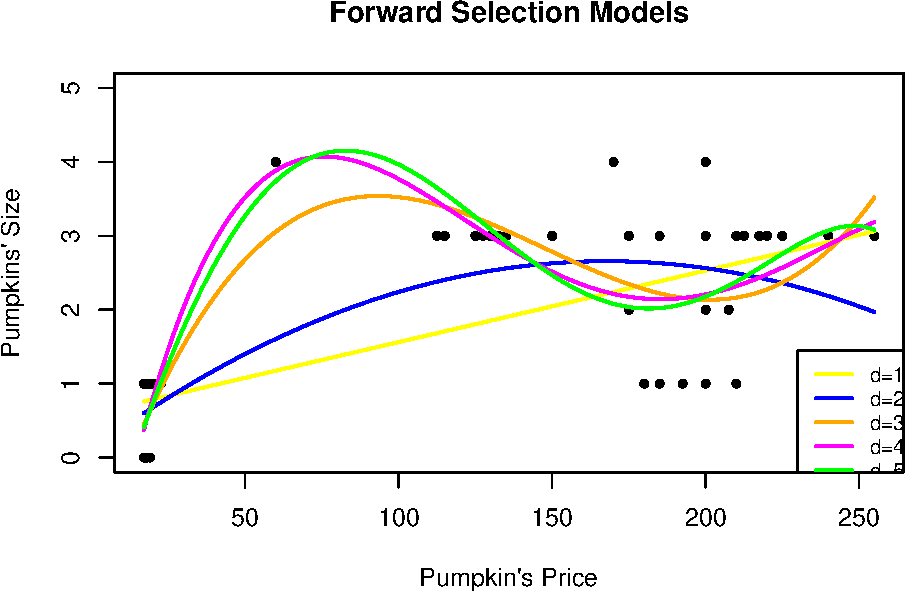
\includegraphics[keepaspectratio]{_main_files/figure-latex/unnamed-chunk-101-1.pdf}}
The magenta line is the one that corresponds to the 4th order model.

\begin{enumerate}
\def\labelenumi{(\arabic{enumi})}
\setcounter{enumi}{1}
\tightlist
\item
  We can also select \(d\) using the Backward Elimination approach, that is we start with a large value for \(d\) and we eliminate terms \emph{until the highest order term in the model is statistically significant}:
\end{enumerate}

\begin{Shaded}
\begin{Highlighting}[]
\NormalTok{lm.pumpkins10 }\OtherTok{=}  \FunctionTok{lm}\NormalTok{(size }\SpecialCharTok{\textasciitilde{}}\NormalTok{ price }\SpecialCharTok{+} \FunctionTok{I}\NormalTok{(price}\SpecialCharTok{\^{}}\DecValTok{2}\NormalTok{) }\SpecialCharTok{+} \FunctionTok{I}\NormalTok{(price}\SpecialCharTok{\^{}}\DecValTok{3}\NormalTok{) }\SpecialCharTok{+} \FunctionTok{I}\NormalTok{(price}\SpecialCharTok{\^{}}\DecValTok{4}\NormalTok{)}\SpecialCharTok{+} \FunctionTok{I}\NormalTok{(price}\SpecialCharTok{\^{}}\DecValTok{5}\NormalTok{)}\SpecialCharTok{+} \FunctionTok{I}\NormalTok{(price}\SpecialCharTok{\^{}}\DecValTok{6}\NormalTok{) }\SpecialCharTok{+} \FunctionTok{I}\NormalTok{(price}\SpecialCharTok{\^{}}\DecValTok{7}\NormalTok{)}\SpecialCharTok{+} \FunctionTok{I}\NormalTok{(price}\SpecialCharTok{\^{}}\DecValTok{8}\NormalTok{)}\SpecialCharTok{+} \FunctionTok{I}\NormalTok{(price}\SpecialCharTok{\^{}}\DecValTok{9}\NormalTok{)}\SpecialCharTok{+} \FunctionTok{I}\NormalTok{(price}\SpecialCharTok{\^{}}\DecValTok{10}\NormalTok{), }\AttributeTok{data=}\NormalTok{pumpkins)}
\FunctionTok{summary}\NormalTok{(lm.pumpkins10)}
\end{Highlighting}
\end{Shaded}

\begin{verbatim}
## 
## Call:
## lm(formula = size ~ price + I(price^2) + I(price^3) + I(price^4) + 
##     I(price^5) + I(price^6) + I(price^7) + I(price^8) + I(price^9) + 
##     I(price^10), data = pumpkins)
## 
## Residuals:
##      Min       1Q   Median       3Q      Max 
## -1.44082 -0.45530 -0.01853  0.53535  2.12546 
## 
## Coefficients:
##               Estimate Std. Error t value Pr(>|t|)
## (Intercept)  1.331e+01  2.671e+01   0.498    0.619
## price       -2.191e+00  4.274e+00  -0.513    0.609
## I(price^2)   1.396e-01  2.625e-01   0.532    0.595
## I(price^3)  -4.389e-03  8.140e-03  -0.539    0.590
## I(price^4)   8.198e-05  1.458e-04   0.562    0.575
## I(price^5)  -9.818e-07  1.624e-06  -0.605    0.546
## I(price^6)   7.731e-09  1.163e-08   0.664    0.507
## I(price^7)  -3.970e-11  5.374e-11  -0.739    0.461
## I(price^8)   1.276e-13  1.549e-13   0.824    0.411
## I(price^9)  -2.321e-16  2.535e-16  -0.916    0.361
## I(price^10)  1.821e-19  1.800e-19   1.012    0.313
## 
## Residual standard error: 0.6483 on 237 degrees of freedom
## Multiple R-squared:  0.7509, Adjusted R-squared:  0.7404 
## F-statistic: 71.45 on 10 and 237 DF,  p-value: < 2.2e-16
\end{verbatim}

\begin{Shaded}
\begin{Highlighting}[]
\NormalTok{lm.pumpkins9 }\OtherTok{=}  \FunctionTok{lm}\NormalTok{(size }\SpecialCharTok{\textasciitilde{}}\NormalTok{ price }\SpecialCharTok{+} \FunctionTok{I}\NormalTok{(price}\SpecialCharTok{\^{}}\DecValTok{2}\NormalTok{) }\SpecialCharTok{+} \FunctionTok{I}\NormalTok{(price}\SpecialCharTok{\^{}}\DecValTok{3}\NormalTok{) }\SpecialCharTok{+} \FunctionTok{I}\NormalTok{(price}\SpecialCharTok{\^{}}\DecValTok{4}\NormalTok{)}\SpecialCharTok{+} \FunctionTok{I}\NormalTok{(price}\SpecialCharTok{\^{}}\DecValTok{5}\NormalTok{)}\SpecialCharTok{+} \FunctionTok{I}\NormalTok{(price}\SpecialCharTok{\^{}}\DecValTok{6}\NormalTok{) }\SpecialCharTok{+} \FunctionTok{I}\NormalTok{(price}\SpecialCharTok{\^{}}\DecValTok{7}\NormalTok{)}\SpecialCharTok{+} \FunctionTok{I}\NormalTok{(price}\SpecialCharTok{\^{}}\DecValTok{8}\NormalTok{)}\SpecialCharTok{+} \FunctionTok{I}\NormalTok{(price}\SpecialCharTok{\^{}}\DecValTok{9}\NormalTok{), }\AttributeTok{data=}\NormalTok{pumpkins)}
\FunctionTok{summary}\NormalTok{(lm.pumpkins9)}
\end{Highlighting}
\end{Shaded}

\begin{verbatim}
## 
## Call:
## lm(formula = size ~ price + I(price^2) + I(price^3) + I(price^4) + 
##     I(price^5) + I(price^6) + I(price^7) + I(price^8) + I(price^9), 
##     data = pumpkins)
## 
## Residuals:
##     Min      1Q  Median      3Q     Max 
## -1.4514 -0.4230 -0.0091  0.5177  2.1072 
## 
## Coefficients:
##               Estimate Std. Error t value Pr(>|t|)  
## (Intercept) -1.191e+01  9.589e+00  -1.242   0.2154  
## price        1.877e+00  1.450e+00   1.295   0.1967  
## I(price^2)  -1.125e-01  8.271e-02  -1.360   0.1751  
## I(price^3)   3.506e-03  2.316e-03   1.514   0.1314  
## I(price^4)  -6.094e-05  3.623e-05  -1.682   0.0939 .
## I(price^5)   6.252e-07  3.391e-07   1.844   0.0664 .
## I(price^6)  -3.875e-09  1.945e-09  -1.993   0.0475 *
## I(price^7)   1.425e-11  6.704e-12   2.125   0.0346 *
## I(price^8)  -2.859e-14  1.276e-14  -2.241   0.0259 *
## I(price^9)   2.411e-17  1.030e-17   2.340   0.0201 *
## ---
## Signif. codes:  0 '***' 0.001 '**' 0.01 '*' 0.05 '.' 0.1 ' ' 1
## 
## Residual standard error: 0.6483 on 238 degrees of freedom
## Multiple R-squared:  0.7499, Adjusted R-squared:  0.7404 
## F-statistic: 79.27 on 9 and 238 DF,  p-value: < 2.2e-16
\end{verbatim}

\begin{Shaded}
\begin{Highlighting}[]
\NormalTok{lm.pumpkins8 }\OtherTok{=}  \FunctionTok{lm}\NormalTok{(size }\SpecialCharTok{\textasciitilde{}}\NormalTok{ price }\SpecialCharTok{+} \FunctionTok{I}\NormalTok{(price}\SpecialCharTok{\^{}}\DecValTok{2}\NormalTok{) }\SpecialCharTok{+} \FunctionTok{I}\NormalTok{(price}\SpecialCharTok{\^{}}\DecValTok{3}\NormalTok{)}\SpecialCharTok{+} \FunctionTok{I}\NormalTok{(price}\SpecialCharTok{\^{}}\DecValTok{4}\NormalTok{)}\SpecialCharTok{+} \FunctionTok{I}\NormalTok{(price}\SpecialCharTok{\^{}}\DecValTok{5}\NormalTok{)}\SpecialCharTok{+} \FunctionTok{I}\NormalTok{(price}\SpecialCharTok{\^{}}\DecValTok{6}\NormalTok{) }\SpecialCharTok{+} \FunctionTok{I}\NormalTok{(price}\SpecialCharTok{\^{}}\DecValTok{7}\NormalTok{)}\SpecialCharTok{+} \FunctionTok{I}\NormalTok{(price}\SpecialCharTok{\^{}}\DecValTok{8}\NormalTok{), }\AttributeTok{data=}\NormalTok{pumpkins)}
\FunctionTok{summary}\NormalTok{(lm.pumpkins8)}
\end{Highlighting}
\end{Shaded}

\begin{verbatim}
## 
## Call:
## lm(formula = size ~ price + I(price^2) + I(price^3) + I(price^4) + 
##     I(price^5) + I(price^6) + I(price^7) + I(price^8), data = pumpkins)
## 
## Residuals:
##      Min       1Q   Median       3Q      Max 
## -1.39988 -0.45678 -0.05827  0.53309  2.02119 
## 
## Coefficients:
##               Estimate Std. Error t value Pr(>|t|)    
## (Intercept)  9.140e+00  3.347e+00   2.731 0.006791 ** 
## price       -1.368e+00  4.257e-01  -3.215 0.001486 ** 
## I(price^2)   7.522e-02  2.032e-02   3.702 0.000266 ***
## I(price^3)  -1.798e-03  4.783e-04  -3.759 0.000214 ***
## I(price^4)   2.262e-05  6.154e-06   3.675 0.000293 ***
## I(price^5)  -1.611e-07  4.541e-08  -3.549 0.000466 ***
## I(price^6)   6.535e-10  1.918e-10   3.407 0.000771 ***
## I(price^7)  -1.406e-12  4.316e-13  -3.259 0.001282 ** 
## I(price^8)   1.246e-15  4.008e-16   3.108 0.002112 ** 
## ---
## Signif. codes:  0 '***' 0.001 '**' 0.01 '*' 0.05 '.' 0.1 ' ' 1
## 
## Residual standard error: 0.6544 on 239 degrees of freedom
## Multiple R-squared:  0.7441, Adjusted R-squared:  0.7355 
## F-statistic: 86.87 on 8 and 239 DF,  p-value: < 2.2e-16
\end{verbatim}

Starting with an order \emph{10} model, we identify that an \emph{9th} order model is \emph{optimal} according to the backward elimination criterion. If we plot all the fitted models, we have:

\begin{Shaded}
\begin{Highlighting}[]
\NormalTok{newprice }\OtherTok{=} \FunctionTok{data.frame}\NormalTok{(}\AttributeTok{price=}\FunctionTok{seq}\NormalTok{(}\DecValTok{17}\NormalTok{, }\DecValTok{255}\NormalTok{, }\DecValTok{1}\NormalTok{))}
\FunctionTok{plot}\NormalTok{(pumpkins}\SpecialCharTok{$}\NormalTok{price, pumpkins}\SpecialCharTok{$}\NormalTok{size, }\AttributeTok{ylim=}\FunctionTok{c}\NormalTok{(}\DecValTok{0}\NormalTok{,}\DecValTok{5}\NormalTok{), }\AttributeTok{pch=}\DecValTok{20}\NormalTok{, }\AttributeTok{xlab=}\StringTok{"Pumpkin\textquotesingle{}s Price"}\NormalTok{, }\AttributeTok{ylab=}\StringTok{"Pumpkins\textquotesingle{} Size"}\NormalTok{, }\AttributeTok{main=}\StringTok{"Backward Selection Models"}\NormalTok{)}
\FunctionTok{lines}\NormalTok{(newprice}\SpecialCharTok{$}\NormalTok{price, }\FunctionTok{predict}\NormalTok{(lm.pumpkins10, newprice), }\AttributeTok{col=}\StringTok{"blue"}\NormalTok{, }\AttributeTok{lty=}\DecValTok{2}\NormalTok{, }\AttributeTok{lwd=}\DecValTok{2}\NormalTok{);}
\FunctionTok{lines}\NormalTok{(newprice}\SpecialCharTok{$}\NormalTok{price, }\FunctionTok{predict}\NormalTok{(lm.pumpkins9, newprice), }\AttributeTok{col=}\StringTok{"orange"}\NormalTok{, }\AttributeTok{lty=}\DecValTok{2}\NormalTok{, }\AttributeTok{lwd=}\DecValTok{2}\NormalTok{);}
\FunctionTok{lines}\NormalTok{(newprice}\SpecialCharTok{$}\NormalTok{price, }\FunctionTok{predict}\NormalTok{(lm.pumpkins8, newprice), }\AttributeTok{col=}\StringTok{"magenta"}\NormalTok{, }\AttributeTok{lty=}\DecValTok{2}\NormalTok{, }\AttributeTok{lwd=}\DecValTok{2}\NormalTok{);}
\FunctionTok{legend}\NormalTok{(}\DecValTok{226}\NormalTok{, }\DecValTok{1}\NormalTok{, }\AttributeTok{legend=}\FunctionTok{c}\NormalTok{(}\StringTok{"d=10"}\NormalTok{, }\StringTok{"d=9"}\NormalTok{, }\StringTok{"d=8"}\NormalTok{),}
       \AttributeTok{col=}\FunctionTok{c}\NormalTok{(}\StringTok{"blue"}\NormalTok{, }\StringTok{"orange"}\NormalTok{, }\StringTok{"magenta"}\NormalTok{), }\AttributeTok{lty=}\FunctionTok{c}\NormalTok{(}\DecValTok{2}\NormalTok{,}\DecValTok{2}\NormalTok{,}\DecValTok{2}\NormalTok{), }\AttributeTok{cex=}\FloatTok{0.8}\NormalTok{, }\AttributeTok{lwd=}\DecValTok{2}\NormalTok{)}
\end{Highlighting}
\end{Shaded}

\pandocbounded{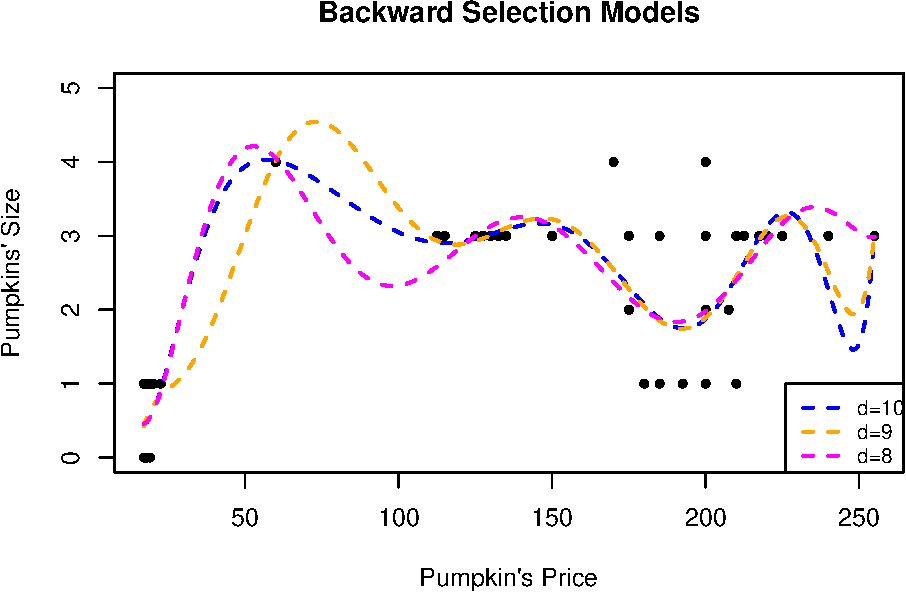
\includegraphics[keepaspectratio]{_main_files/figure-latex/unnamed-chunk-103-1.pdf}}

The magenta line is the one that corresponds to the \emph{9th} order model.

For the fitted model we finally choose, we should (as always) perform diagnostic tests.

\subsection{Orthogonal Polynomials}\label{orthogonal-polynomials}

Fitting high order polynomials is generally \textbf{not recommended}, since they are very \emph{unstable} and \emph{difficult to interpret}. In addition, successive predictors \(x^j\) are \emph{highly correlated} introducing multicollinearity problems. One way around this is to fit \textbf{orthogonal polynomials} of the form:
\[y_i=\beta_0+\beta_1z_1+\ldots+\beta_d z_d+\varepsilon_i\]
where each \(z_j=a_{1} + b_{2} x + \ldots+ \kappa_j x^j\) is a polynomial of order \(j\) with coefficients chosen such that \(z_i^\top z_j=0\) (i.e.~the inner product of any two polynomials is zero).

\textbf{The Chicago Pumpkins Example}

In \texttt{R}, we can fit orthogonal polynomials using the \texttt{poly} function. In the code below, we repeat the same process as before (for choosing \(d\)) using the orthogonal polynomials.

\begin{Shaded}
\begin{Highlighting}[]
\CommentTok{\# Forward Selection}
\NormalTok{lm.pumpkinsO2 }\OtherTok{=}  \FunctionTok{lm}\NormalTok{(size }\SpecialCharTok{\textasciitilde{}} \FunctionTok{poly}\NormalTok{(price,}\DecValTok{2}\NormalTok{), }\AttributeTok{data=}\NormalTok{pumpkins)}
\FunctionTok{summary}\NormalTok{(lm.pumpkinsO2)}
\end{Highlighting}
\end{Shaded}

\begin{verbatim}
## 
## Call:
## lm(formula = size ~ poly(price, 2), data = pumpkins)
## 
## Residuals:
##     Min      1Q  Median      3Q     Max 
## -1.6438 -0.6029  0.3695  0.4895  2.3941 
## 
## Coefficients:
##                 Estimate Std. Error t value Pr(>|t|)    
## (Intercept)      1.70161    0.05559  30.612  < 2e-16 ***
## poly(price, 2)1 13.37846    0.87538  15.283  < 2e-16 ***
## poly(price, 2)2 -5.76139    0.87538  -6.582  2.8e-10 ***
## ---
## Signif. codes:  0 '***' 0.001 '**' 0.01 '*' 0.05 '.' 0.1 ' ' 1
## 
## Residual standard error: 0.8754 on 245 degrees of freedom
## Multiple R-squared:  0.5305, Adjusted R-squared:  0.5267 
## F-statistic: 138.4 on 2 and 245 DF,  p-value: < 2.2e-16
\end{verbatim}

\begin{Shaded}
\begin{Highlighting}[]
\NormalTok{lm.pumpkinsO3 }\OtherTok{=}  \FunctionTok{lm}\NormalTok{(size }\SpecialCharTok{\textasciitilde{}} \FunctionTok{poly}\NormalTok{(price,}\DecValTok{3}\NormalTok{), }\AttributeTok{data=}\NormalTok{pumpkins)}
\FunctionTok{summary}\NormalTok{(lm.pumpkinsO3)}
\end{Highlighting}
\end{Shaded}

\begin{verbatim}
## 
## Call:
## lm(formula = size ~ poly(price, 3), data = pumpkins)
## 
## Residuals:
##     Min      1Q  Median      3Q     Max 
## -1.2786 -0.4937 -0.1368  0.5531  1.8633 
## 
## Coefficients:
##                 Estimate Std. Error t value Pr(>|t|)    
## (Intercept)       1.7016     0.0456  37.313  < 2e-16 ***
## poly(price, 3)1  13.3785     0.7182  18.628  < 2e-16 ***
## poly(price, 3)2  -5.7614     0.7182  -8.022 4.35e-14 ***
## poly(price, 3)3   7.8672     0.7182  10.954  < 2e-16 ***
## ---
## Signif. codes:  0 '***' 0.001 '**' 0.01 '*' 0.05 '.' 0.1 ' ' 1
## 
## Residual standard error: 0.7182 on 244 degrees of freedom
## Multiple R-squared:  0.6853, Adjusted R-squared:  0.6814 
## F-statistic: 177.1 on 3 and 244 DF,  p-value: < 2.2e-16
\end{verbatim}

\begin{Shaded}
\begin{Highlighting}[]
\NormalTok{lm.pumpkinsO4 }\OtherTok{=}  \FunctionTok{lm}\NormalTok{(size }\SpecialCharTok{\textasciitilde{}} \FunctionTok{poly}\NormalTok{(price,}\DecValTok{4}\NormalTok{), }\AttributeTok{data=}\NormalTok{pumpkins)}
\FunctionTok{summary}\NormalTok{(lm.pumpkinsO4)}
\end{Highlighting}
\end{Shaded}

\begin{verbatim}
## 
## Call:
## lm(formula = size ~ poly(price, 4), data = pumpkins)
## 
## Residuals:
##     Min      1Q  Median      3Q     Max 
## -1.3200 -0.4497 -0.1241  0.5539  1.7925 
## 
## Coefficients:
##                 Estimate Std. Error t value Pr(>|t|)    
## (Intercept)      1.70161    0.04407  38.608  < 2e-16 ***
## poly(price, 4)1 13.37846    0.69408  19.275  < 2e-16 ***
## poly(price, 4)2 -5.76139    0.69408  -8.301 7.22e-15 ***
## poly(price, 4)3  7.86718    0.69408  11.335  < 2e-16 ***
## poly(price, 4)4 -2.96423    0.69408  -4.271 2.80e-05 ***
## ---
## Signif. codes:  0 '***' 0.001 '**' 0.01 '*' 0.05 '.' 0.1 ' ' 1
## 
## Residual standard error: 0.6941 on 243 degrees of freedom
## Multiple R-squared:  0.7073, Adjusted R-squared:  0.7025 
## F-statistic: 146.8 on 4 and 243 DF,  p-value: < 2.2e-16
\end{verbatim}

\begin{Shaded}
\begin{Highlighting}[]
\NormalTok{lm.pumpkinsO5 }\OtherTok{=}  \FunctionTok{lm}\NormalTok{(size }\SpecialCharTok{\textasciitilde{}} \FunctionTok{poly}\NormalTok{(price,}\DecValTok{5}\NormalTok{), }\AttributeTok{data=}\NormalTok{pumpkins)}
\FunctionTok{summary}\NormalTok{(lm.pumpkinsO5)}
\end{Highlighting}
\end{Shaded}

\begin{verbatim}
## 
## Call:
## lm(formula = size ~ poly(price, 5), data = pumpkins)
## 
## Residuals:
##      Min       1Q   Median       3Q      Max 
## -1.38082 -0.46537 -0.08211  0.53463  1.91954 
## 
## Coefficients:
##                 Estimate Std. Error t value Pr(>|t|)    
## (Intercept)      1.70161    0.04382  38.831  < 2e-16 ***
## poly(price, 5)1 13.37846    0.69009  19.387  < 2e-16 ***
## poly(price, 5)2 -5.76139    0.69009  -8.349 5.35e-15 ***
## poly(price, 5)3  7.86718    0.69009  11.400  < 2e-16 ***
## poly(price, 5)4 -2.96423    0.69009  -4.295 2.53e-05 ***
## poly(price, 5)5 -1.34841    0.69009  -1.954   0.0519 .  
## ---
## Signif. codes:  0 '***' 0.001 '**' 0.01 '*' 0.05 '.' 0.1 ' ' 1
## 
## Residual standard error: 0.6901 on 242 degrees of freedom
## Multiple R-squared:  0.7118, Adjusted R-squared:  0.7059 
## F-statistic: 119.6 on 5 and 242 DF,  p-value: < 2.2e-16
\end{verbatim}

\begin{Shaded}
\begin{Highlighting}[]
\NormalTok{newprice }\OtherTok{=} \FunctionTok{data.frame}\NormalTok{(}\AttributeTok{price=}\FunctionTok{seq}\NormalTok{(}\DecValTok{17}\NormalTok{, }\DecValTok{255}\NormalTok{, }\DecValTok{1}\NormalTok{))}
\FunctionTok{plot}\NormalTok{(pumpkins}\SpecialCharTok{$}\NormalTok{price, pumpkins}\SpecialCharTok{$}\NormalTok{size, }\AttributeTok{pch=}\DecValTok{20}\NormalTok{,  }\AttributeTok{ylim=}\FunctionTok{c}\NormalTok{(}\DecValTok{0}\NormalTok{,}\DecValTok{5}\NormalTok{),}\AttributeTok{xlab=}\StringTok{"Pumpkin\textquotesingle{}s Price"}\NormalTok{, }\AttributeTok{ylab=}\StringTok{"Pumpkins\textquotesingle{} Size"}\NormalTok{, }\AttributeTok{main=}\StringTok{"Forward Selection Models: Orthogonal Polynomials"}\NormalTok{)}
\FunctionTok{lines}\NormalTok{(newprice}\SpecialCharTok{$}\NormalTok{price, }\FunctionTok{predict}\NormalTok{(lm.pumpkinsO2, newprice), }\AttributeTok{col=}\StringTok{"blue"}\NormalTok{, }\AttributeTok{lty=}\DecValTok{1}\NormalTok{, }\AttributeTok{lwd=}\DecValTok{2}\NormalTok{);}
\FunctionTok{lines}\NormalTok{(newprice}\SpecialCharTok{$}\NormalTok{price, }\FunctionTok{predict}\NormalTok{(lm.pumpkinsO3, newprice), }\AttributeTok{col=}\StringTok{"orange"}\NormalTok{, }\AttributeTok{lty=}\DecValTok{1}\NormalTok{, }\AttributeTok{lwd=}\DecValTok{2}\NormalTok{);}
\FunctionTok{lines}\NormalTok{(newprice}\SpecialCharTok{$}\NormalTok{price, }\FunctionTok{predict}\NormalTok{(lm.pumpkinsO4, newprice), }\AttributeTok{col=}\StringTok{"magenta"}\NormalTok{, }\AttributeTok{lty=}\DecValTok{1}\NormalTok{, }\AttributeTok{lwd=}\DecValTok{2}\NormalTok{);}
\FunctionTok{lines}\NormalTok{(newprice}\SpecialCharTok{$}\NormalTok{price, }\FunctionTok{predict}\NormalTok{(lm.pumpkinsO5, newprice), }\AttributeTok{col=}\StringTok{"green"}\NormalTok{, }\AttributeTok{lty=}\DecValTok{1}\NormalTok{, }\AttributeTok{lwd=}\DecValTok{2}\NormalTok{);}
\FunctionTok{legend}\NormalTok{(}\DecValTok{230}\NormalTok{, }\FloatTok{1.3}\NormalTok{, }\AttributeTok{legend=}\FunctionTok{c}\NormalTok{(}\StringTok{"d=2"}\NormalTok{, }\StringTok{"d=3"}\NormalTok{, }\StringTok{"d=4"}\NormalTok{, }\StringTok{"d=5"}\NormalTok{),}
       \AttributeTok{col=}\FunctionTok{c}\NormalTok{(}\StringTok{"blue"}\NormalTok{, }\StringTok{"orange"}\NormalTok{, }\StringTok{"magenta"}\NormalTok{, }\StringTok{"green"}\NormalTok{), }\AttributeTok{lty=}\FunctionTok{c}\NormalTok{(}\DecValTok{1}\NormalTok{,}\DecValTok{1}\NormalTok{,}\DecValTok{1}\NormalTok{,}\DecValTok{1}\NormalTok{), }\AttributeTok{cex=}\FloatTok{0.8}\NormalTok{, }\AttributeTok{lwd=}\FunctionTok{c}\NormalTok{(}\DecValTok{2}\NormalTok{,}\DecValTok{2}\NormalTok{,}\DecValTok{2}\NormalTok{,}\DecValTok{2}\NormalTok{))}
\end{Highlighting}
\end{Shaded}

\pandocbounded{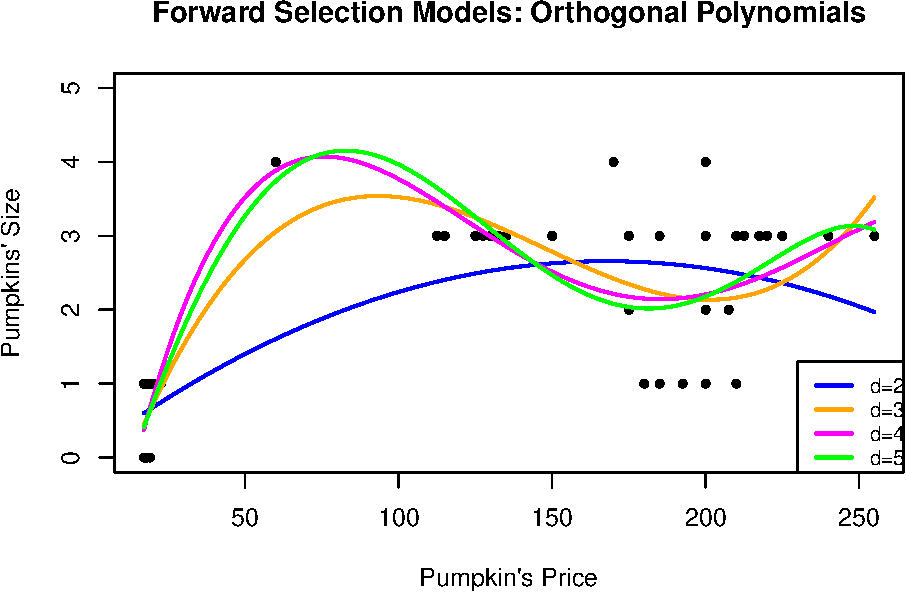
\includegraphics[keepaspectratio]{_main_files/figure-latex/unnamed-chunk-104-1.pdf}}

\begin{Shaded}
\begin{Highlighting}[]
\CommentTok{\# Backward Selection}
\NormalTok{lm.pumpkinsO10 }\OtherTok{=}  \FunctionTok{lm}\NormalTok{(size }\SpecialCharTok{\textasciitilde{}} \FunctionTok{poly}\NormalTok{(price,}\DecValTok{10}\NormalTok{), }\AttributeTok{data=}\NormalTok{pumpkins)}
\FunctionTok{summary}\NormalTok{(lm.pumpkinsO10)}
\end{Highlighting}
\end{Shaded}

\begin{verbatim}
## 
## Call:
## lm(formula = size ~ poly(price, 10), data = pumpkins)
## 
## Residuals:
##      Min       1Q   Median       3Q      Max 
## -1.44082 -0.45530 -0.01853  0.53535  2.12546 
## 
## Coefficients:
##                   Estimate Std. Error t value Pr(>|t|)    
## (Intercept)        1.70161    0.04117  41.335  < 2e-16 ***
## poly(price, 10)1  13.37846    0.64829  20.636  < 2e-16 ***
## poly(price, 10)2  -5.76139    0.64829  -8.887  < 2e-16 ***
## poly(price, 10)3   7.86718    0.64829  12.135  < 2e-16 ***
## poly(price, 10)4  -2.96423    0.64829  -4.572 7.77e-06 ***
## poly(price, 10)5  -1.34841    0.64829  -2.080  0.03861 *  
## poly(price, 10)6  -1.45456    0.64829  -2.244  0.02578 *  
## poly(price, 10)7  -2.57955    0.64829  -3.979 9.20e-05 ***
## poly(price, 10)8   2.03378    0.64829   3.137  0.00192 ** 
## poly(price, 10)9   1.51698    0.64829   2.340  0.02012 *  
## poly(price, 10)10  0.65591    0.64829   1.012  0.31269    
## ---
## Signif. codes:  0 '***' 0.001 '**' 0.01 '*' 0.05 '.' 0.1 ' ' 1
## 
## Residual standard error: 0.6483 on 237 degrees of freedom
## Multiple R-squared:  0.7509, Adjusted R-squared:  0.7404 
## F-statistic: 71.45 on 10 and 237 DF,  p-value: < 2.2e-16
\end{verbatim}

\begin{Shaded}
\begin{Highlighting}[]
\NormalTok{lm.pumpkinsO9 }\OtherTok{=}  \FunctionTok{lm}\NormalTok{(size }\SpecialCharTok{\textasciitilde{}} \FunctionTok{poly}\NormalTok{(price,}\DecValTok{9}\NormalTok{), }\AttributeTok{data=}\NormalTok{pumpkins)}
\FunctionTok{summary}\NormalTok{(lm.pumpkinsO9)}
\end{Highlighting}
\end{Shaded}

\begin{verbatim}
## 
## Call:
## lm(formula = size ~ poly(price, 9), data = pumpkins)
## 
## Residuals:
##     Min      1Q  Median      3Q     Max 
## -1.4514 -0.4230 -0.0091  0.5177  2.1072 
## 
## Coefficients:
##                 Estimate Std. Error t value Pr(>|t|)    
## (Intercept)      1.70161    0.04117  41.333  < 2e-16 ***
## poly(price, 9)1 13.37846    0.64833  20.635  < 2e-16 ***
## poly(price, 9)2 -5.76139    0.64833  -8.887  < 2e-16 ***
## poly(price, 9)3  7.86718    0.64833  12.135  < 2e-16 ***
## poly(price, 9)4 -2.96423    0.64833  -4.572 7.76e-06 ***
## poly(price, 9)5 -1.34841    0.64833  -2.080  0.03861 *  
## poly(price, 9)6 -1.45456    0.64833  -2.244  0.02578 *  
## poly(price, 9)7 -2.57955    0.64833  -3.979 9.20e-05 ***
## poly(price, 9)8  2.03378    0.64833   3.137  0.00192 ** 
## poly(price, 9)9  1.51698    0.64833   2.340  0.02012 *  
## ---
## Signif. codes:  0 '***' 0.001 '**' 0.01 '*' 0.05 '.' 0.1 ' ' 1
## 
## Residual standard error: 0.6483 on 238 degrees of freedom
## Multiple R-squared:  0.7499, Adjusted R-squared:  0.7404 
## F-statistic: 79.27 on 9 and 238 DF,  p-value: < 2.2e-16
\end{verbatim}

\begin{Shaded}
\begin{Highlighting}[]
\NormalTok{lm.pumpkinsO8 }\OtherTok{=}  \FunctionTok{lm}\NormalTok{(size }\SpecialCharTok{\textasciitilde{}} \FunctionTok{poly}\NormalTok{(price,}\DecValTok{8}\NormalTok{), }\AttributeTok{data=}\NormalTok{pumpkins)}
\FunctionTok{summary}\NormalTok{(lm.pumpkinsO8)}
\end{Highlighting}
\end{Shaded}

\begin{verbatim}
## 
## Call:
## lm(formula = size ~ poly(price, 8), data = pumpkins)
## 
## Residuals:
##      Min       1Q   Median       3Q      Max 
## -1.39988 -0.45678 -0.05827  0.53309  2.02119 
## 
## Coefficients:
##                 Estimate Std. Error t value Pr(>|t|)    
## (Intercept)      1.70161    0.04155  40.951  < 2e-16 ***
## poly(price, 8)1 13.37846    0.65437  20.445  < 2e-16 ***
## poly(price, 8)2 -5.76139    0.65437  -8.805 2.71e-16 ***
## poly(price, 8)3  7.86718    0.65437  12.023  < 2e-16 ***
## poly(price, 8)4 -2.96423    0.65437  -4.530 9.32e-06 ***
## poly(price, 8)5 -1.34841    0.65437  -2.061 0.040421 *  
## poly(price, 8)6 -1.45456    0.65437  -2.223 0.027162 *  
## poly(price, 8)7 -2.57955    0.65437  -3.942 0.000106 ***
## poly(price, 8)8  2.03378    0.65437   3.108 0.002112 ** 
## ---
## Signif. codes:  0 '***' 0.001 '**' 0.01 '*' 0.05 '.' 0.1 ' ' 1
## 
## Residual standard error: 0.6544 on 239 degrees of freedom
## Multiple R-squared:  0.7441, Adjusted R-squared:  0.7355 
## F-statistic: 86.87 on 8 and 239 DF,  p-value: < 2.2e-16
\end{verbatim}

\begin{Shaded}
\begin{Highlighting}[]
\FunctionTok{plot}\NormalTok{(pumpkins}\SpecialCharTok{$}\NormalTok{price, pumpkins}\SpecialCharTok{$}\NormalTok{size, }\AttributeTok{pch=}\DecValTok{20}\NormalTok{, }\AttributeTok{ylim=}\FunctionTok{c}\NormalTok{(}\DecValTok{0}\NormalTok{,}\DecValTok{5}\NormalTok{), }\AttributeTok{xlab=}\StringTok{"Pumpkin\textquotesingle{}s Price"}\NormalTok{, }\AttributeTok{ylab=}\StringTok{"Pumpkins\textquotesingle{} Size"}\NormalTok{, }\AttributeTok{main=}\StringTok{"Backward Selection Models: Orthogonal Polynomials"}\NormalTok{)}
\FunctionTok{lines}\NormalTok{(newprice}\SpecialCharTok{$}\NormalTok{price, }\FunctionTok{predict}\NormalTok{(lm.pumpkinsO10, newprice), }\AttributeTok{col=}\StringTok{"blue"}\NormalTok{, }\AttributeTok{lty=}\DecValTok{2}\NormalTok{, }\AttributeTok{lwd=}\DecValTok{2}\NormalTok{);}
\FunctionTok{lines}\NormalTok{(newprice}\SpecialCharTok{$}\NormalTok{price, }\FunctionTok{predict}\NormalTok{(lm.pumpkinsO9, newprice), }\AttributeTok{col=}\StringTok{"orange"}\NormalTok{, }\AttributeTok{lty=}\DecValTok{2}\NormalTok{, }\AttributeTok{lwd=}\DecValTok{2}\NormalTok{);}
\FunctionTok{lines}\NormalTok{(newprice}\SpecialCharTok{$}\NormalTok{price, }\FunctionTok{predict}\NormalTok{(lm.pumpkinsO8, newprice), }\AttributeTok{col=}\StringTok{"magenta"}\NormalTok{, }\AttributeTok{lty=}\DecValTok{2}\NormalTok{, }\AttributeTok{lwd=}\DecValTok{2}\NormalTok{);}
\FunctionTok{legend}\NormalTok{(}\DecValTok{225}\NormalTok{, }\FloatTok{1.2}\NormalTok{, }\AttributeTok{legend=}\FunctionTok{c}\NormalTok{(}\StringTok{"d=10"}\NormalTok{, }\StringTok{"d=9"}\NormalTok{, }\StringTok{"d=8"}\NormalTok{),  }\AttributeTok{col=}\FunctionTok{c}\NormalTok{(}\StringTok{"blue"}\NormalTok{, }\StringTok{"orange"}\NormalTok{, }\StringTok{"magenta"}\NormalTok{), }\AttributeTok{lty=}\FunctionTok{c}\NormalTok{(}\DecValTok{2}\NormalTok{,}\DecValTok{2}\NormalTok{,}\DecValTok{2}\NormalTok{), }\AttributeTok{cex=}\FloatTok{0.8}\NormalTok{, }\AttributeTok{lwd=}\DecValTok{2}\NormalTok{)}
\end{Highlighting}
\end{Shaded}

\pandocbounded{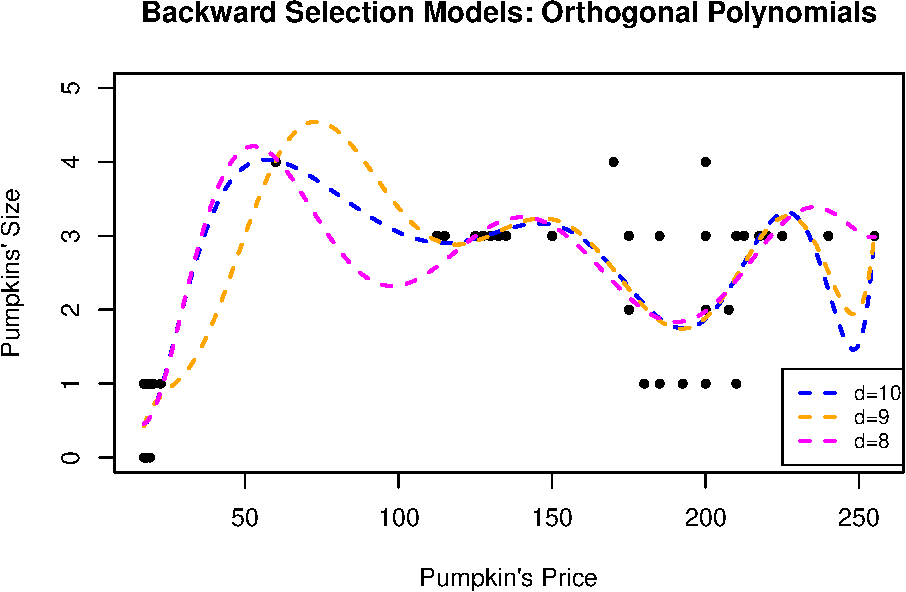
\includegraphics[keepaspectratio]{_main_files/figure-latex/unnamed-chunk-104-2.pdf}}

\subsection{Piece-wise Polynomials}\label{piece-wise-polynomials}

If the true mean of \(\mathbb{E}(Y|X=x) = f(x)\) is \emph{too wiggly}, we might need to fit a higher order polynomial, which is not always a good idea. Instead we consider \textbf{piece-wise polynomials}:

\begin{enumerate}
\def\labelenumi{\arabic{enumi}.}
\item
  we divide the range of \(x\) into several intervals, and
\item
  within each interval, \(f(x)\) is a low-order polynomial, e.g., cubic or quadratic, but the polynomial coefficients will be different from interval to interval
\item
  we require the overall \(f(x)\) to be continuous up to certain derivatives.
\end{enumerate}

This method is also called \emph{``broken-stick regression''}. Its benefit is that it localizes the influence of each data point to a particular segment, but overall it is not a very smooth line as the one we obtain by fitting a single polynomial for the whole data set.

\section{Splines Regression}\label{splines-regression}

\emph{Splines} are piecewise polynomials thar are constructed so that thay can be both sensitive and smooth, but also capture local features of the data.

A \textbf{Cubic Spline} is a curve constructed from sections of cubic polynomials, joined together so that the curve is \emph{continuous up to second derivative}. The points at which the sections join are called the \textbf{knots} of the spline. For a conventional spline, the knots occur wherever there is a datum, but for the regression splines the locations of the knots must be chosen. Typically, the knots would either be \emph{evenly spaced} through the range of observed \(x\) values, or placed at the \emph{quantiles} of the distribution of unique \(x\) values. Each section of cubic has different coefficients, but at the knots \emph{it will match its neighboring sections in value and first two derivatives}.

\textbf{Cubic Splines (Mathematical) Definition}

A function \(g\) defined on \([a,b]\) is a \textbf{cubic spline} with respect to \textbf{knots} \(\{\xi_i\}_{i=1}^m\) (specifically \(a<\xi_1<\xi_2<\ldots<\xi_m<b\)) if:

\begin{itemize}
\item
  \(g\) is a cubic polynomial in each of the \(m+1\) intervals, i.e.
  \[g(x) =d_ix^3+c_ix^2+b_ix+a_i,\quad x\in [\xi_i,\xi_{i+1}]\]
  where \(i=0,\ldots, m\), \(\xi_0=a\) and \(\xi_{m+1}=b\).
\item
  \(g\) is continuous up to the \emph{2nd} derivative. Since \(g\) is continuous up to the \emph{2nd} derivative \emph{for any point inside an interval}, it suffices to check the following conditions:
  \[g^{(0,1,2)} (\xi_i^+)=g^{(0,1,2)}(\xi_i^-),\quad i=1, \ldots, m\]
  This expression indicates that the function and the first and second order derivatives are continuous at the knots.
\end{itemize}

\textbf{How many free parameters do we need to represent a cubic spline?}

\textbf{(+)} 4 parameters \((d_i,c_i,b_i,a_i)\) \emph{for each of the \((m+1)\) intervals}.

\textbf{(-)} 3 constraints \emph{at each of the \(m\) knots} (continuity constraints).

The total number of free parameters (similar to the number of degrees of freedom) is:
\[4(m+1) - 3m = m + 4\]

\textbf{A property of the cubic splines}

Suppose the knots \(\{\xi_i\}_{i=1}^m\) are given.

\begin{itemize}
\tightlist
\item
  If \(g_1(x)\) and \(g_2(x)\) are cubic splines, the linear combination
  \[a_1g_1(x)+a_2g_2(x)\]
  is also a cubic spline, where \(a_1\) and \(a_2\) are known constants.
\end{itemize}

That is, for a set of given knots, the corresponding \emph{cubic splines form a linear space (of functions) with dim \((m + 4)\)}.

\subsection{Examples of Cubic Splines Basis}\label{examples-of-cubic-splines-basis}

\begin{enumerate}
\def\labelenumi{\arabic{enumi}.}
\tightlist
\item
  A set of basis functions for cubic splines (w.r.t knots \(\{\xi_i\}_{i=1}^m\)) is given by:
  \begin{align*}
    h_0(x)&= 1\\
     h_1(x)&=x\\
    h_2(x)&=x^2\\
    h_3(x)&=x^3;\\
    h_{i+3}(x) &= (x-\xi_i)_+^3,\quad i=1,2,\ldots,m\\
  \end{align*}
  That is, any cubic spline can be uniquely expressed as:
  \[ \beta_0 +\sum_{j=1}^{m+3}\beta_j h_j(x)\]
\end{enumerate}

\begin{enumerate}
\def\labelenumi{\arabic{enumi}.}
\setcounter{enumi}{1}
\tightlist
\item
  Given knot locations, there are many alternative, but equivalent ways of writing down a basis for cubic splines. For example, \emph{another} basis for cubic splines can be written as:
  \begin{align*}
  h_0(x) &= 1\\
  h_1(x) &= x\\
  h_{i+1}(x) &= R(x, \xi_i^*),\,\, i=1, \ldots, q-1
  \end{align*}
  where
  \begin{align*}
  R(x,z) &= \left[  (z-1/2)^2 - 1/12\right] \left[  (x-1/2)^2 - 1/12\right]/4\\
  & \quad \,- \left[  (|x-z|-1/2)^4 - 1/2   (|x-z|-1/2)^2 + 7/240\right] /24\\
  \end{align*}
\end{enumerate}

\textbf{An Example of a Cubic Splines Basis}

We first define the function \(R(x,z)\) as above in \texttt{R}:

\begin{Shaded}
\begin{Highlighting}[]
\NormalTok{R\_xz }\OtherTok{\textless{}{-}} \ControlFlowTok{function}\NormalTok{(x,z)\{}
\NormalTok{  ((z}\FloatTok{{-}0.5}\NormalTok{)}\SpecialCharTok{\^{}}\DecValTok{2{-}1}\SpecialCharTok{/}\DecValTok{12}\NormalTok{)}\SpecialCharTok{*}\NormalTok{((x}\FloatTok{{-}0.5}\NormalTok{)}\SpecialCharTok{\^{}}\DecValTok{2{-}1}\SpecialCharTok{/}\DecValTok{12}\NormalTok{)}\SpecialCharTok{/}\DecValTok{4}\SpecialCharTok{{-}}\NormalTok{((}\FunctionTok{abs}\NormalTok{(x}\SpecialCharTok{{-}}\NormalTok{z)}\SpecialCharTok{{-}}\FloatTok{0.5}\NormalTok{)}\SpecialCharTok{\^{}}\DecValTok{4}\SpecialCharTok{{-}}\NormalTok{(}\FunctionTok{abs}\NormalTok{(x}\SpecialCharTok{{-}}\NormalTok{z)}\SpecialCharTok{{-}}\FloatTok{0.5}\NormalTok{)}\SpecialCharTok{\^{}}\DecValTok{2}\SpecialCharTok{/}\DecValTok{2}\SpecialCharTok{+}\DecValTok{7}\SpecialCharTok{/}\DecValTok{240}\NormalTok{)}\SpecialCharTok{/}\DecValTok{24}
\NormalTok{\}}
\end{Highlighting}
\end{Shaded}

We then need to define the knots

\begin{Shaded}
\begin{Highlighting}[]
\NormalTok{new.knots}\OtherTok{=} \FunctionTok{c}\NormalTok{(}\DecValTok{1}\SpecialCharTok{/}\DecValTok{6}\NormalTok{, }\DecValTok{3}\SpecialCharTok{/}\DecValTok{6}\NormalTok{, }\DecValTok{5}\SpecialCharTok{/}\DecValTok{6}\NormalTok{)}
\end{Highlighting}
\end{Shaded}

In regression examples the \(x\) variable will be the predictor (there is no need to generate any \(x\) values). Here, we need a ``generic'' \(x\) for illustration purposes.

\begin{Shaded}
\begin{Highlighting}[]
\NormalTok{x}\OtherTok{=}\FunctionTok{seq}\NormalTok{(}\DecValTok{0}\NormalTok{, }\DecValTok{1}\NormalTok{, }\AttributeTok{by=}\FloatTok{0.01}\NormalTok{)}
\end{Highlighting}
\end{Shaded}

Finally, we defined the splines functions, based on the definition given above:

\begin{Shaded}
\begin{Highlighting}[]
\NormalTok{spline1 }\OtherTok{=} \FunctionTok{rep}\NormalTok{(}\DecValTok{1}\NormalTok{, }\FunctionTok{length}\NormalTok{(x)) }\CommentTok{\# First basis function}
\NormalTok{spline2 }\OtherTok{=}\NormalTok{ x }\CommentTok{\# Second basis function}
\NormalTok{spline3 }\OtherTok{=} \FunctionTok{R\_xz}\NormalTok{(x,new.knots[}\DecValTok{1}\NormalTok{]) }\CommentTok{\# Third basis function }
\NormalTok{spline4 }\OtherTok{=} \FunctionTok{R\_xz}\NormalTok{(x,new.knots[}\DecValTok{2}\NormalTok{]) }\CommentTok{\# Fourth basis function }
\NormalTok{spline5 }\OtherTok{=} \FunctionTok{R\_xz}\NormalTok{(x,new.knots[}\DecValTok{3}\NormalTok{]) }\CommentTok{\# Fifth basis function }
\end{Highlighting}
\end{Shaded}

If we want to represent a function using the basis above, we have:

\begin{Shaded}
\begin{Highlighting}[]
\NormalTok{fun1s }\OtherTok{=} \DecValTok{4}\SpecialCharTok{*}\NormalTok{spline1 }\SpecialCharTok{{-}} \FloatTok{0.05}\SpecialCharTok{*}\NormalTok{spline2 }\SpecialCharTok{{-}} \DecValTok{6}\SpecialCharTok{*}\NormalTok{spline3 }\SpecialCharTok{+}\DecValTok{2}\SpecialCharTok{*}\NormalTok{spline4 }\SpecialCharTok{+}\DecValTok{10}\SpecialCharTok{*}\NormalTok{spline5}
\end{Highlighting}
\end{Shaded}

For illustration purposes, we plot the basis functions defined above as well as the function \(f\):

\begin{Shaded}
\begin{Highlighting}[]
\FunctionTok{par}\NormalTok{(}\AttributeTok{mfrow =} \FunctionTok{c}\NormalTok{(}\DecValTok{2}\NormalTok{,}\DecValTok{3}\NormalTok{))}
\FunctionTok{plot}\NormalTok{(x, spline1, }\AttributeTok{type=}\StringTok{\textquotesingle{}l\textquotesingle{}}\NormalTok{, }\AttributeTok{lty=}\DecValTok{3}\NormalTok{, }\AttributeTok{ylab=}\FunctionTok{expression}\NormalTok{(}\StringTok{"h"}\NormalTok{[}\DecValTok{0}\NormalTok{]}\SpecialCharTok{*}\StringTok{"(x)=1"}\NormalTok{))}
\FunctionTok{plot}\NormalTok{(x, spline2, }\AttributeTok{type=}\StringTok{\textquotesingle{}l\textquotesingle{}}\NormalTok{,}\AttributeTok{lty=}\DecValTok{3}\NormalTok{, }\AttributeTok{ylab=}\FunctionTok{expression}\NormalTok{(}\StringTok{"h"}\NormalTok{[}\DecValTok{1}\NormalTok{]}\SpecialCharTok{*}\StringTok{"(x)=x"}\NormalTok{))}
\FunctionTok{plot}\NormalTok{(x, spline3, }\AttributeTok{type=}\StringTok{\textquotesingle{}l\textquotesingle{}}\NormalTok{,}\AttributeTok{lty=}\DecValTok{3}\NormalTok{, }\AttributeTok{ylab=}\FunctionTok{expression}\NormalTok{(}\FunctionTok{paste}\NormalTok{(h[}\DecValTok{2}\NormalTok{](x))}\SpecialCharTok{*}\StringTok{"="}\SpecialCharTok{*}\FunctionTok{paste}\NormalTok{(}\FunctionTok{R}\NormalTok{(x,xi[}\DecValTok{1}\NormalTok{])))  )}
\FunctionTok{plot}\NormalTok{(x, spline4, }\AttributeTok{type=}\StringTok{\textquotesingle{}l\textquotesingle{}}\NormalTok{,}\AttributeTok{lty=}\DecValTok{3}\NormalTok{, }\AttributeTok{ylab=}\FunctionTok{expression}\NormalTok{(}\FunctionTok{paste}\NormalTok{(h[}\DecValTok{3}\NormalTok{](x))}\SpecialCharTok{*}\StringTok{"="}\SpecialCharTok{*}\FunctionTok{paste}\NormalTok{(}\FunctionTok{R}\NormalTok{(x,xi[}\DecValTok{2}\NormalTok{])))  )}
\FunctionTok{plot}\NormalTok{(x, spline5, }\AttributeTok{type=}\StringTok{\textquotesingle{}l\textquotesingle{}}\NormalTok{,}\AttributeTok{lty=}\DecValTok{3}\NormalTok{, }\AttributeTok{ylab=}\FunctionTok{expression}\NormalTok{(}\FunctionTok{paste}\NormalTok{(h[}\DecValTok{4}\NormalTok{](x))}\SpecialCharTok{*}\StringTok{"="}\SpecialCharTok{*}\FunctionTok{paste}\NormalTok{(}\FunctionTok{R}\NormalTok{(x,xi[}\DecValTok{3}\NormalTok{])))  )}
\FunctionTok{plot}\NormalTok{(x, fun1s, }\AttributeTok{type=}\StringTok{\textquotesingle{}l\textquotesingle{}}\NormalTok{, }\AttributeTok{ylab=}\StringTok{"f(x)"}\NormalTok{, }\AttributeTok{main=}\FunctionTok{expression}\NormalTok{(}\StringTok{"f(x) =  4 {-} 0.05 h"}\NormalTok{[}\DecValTok{1}\NormalTok{]}\SpecialCharTok{*}\StringTok{" {-} 6 h"}\NormalTok{[}\DecValTok{2}\NormalTok{]}\SpecialCharTok{*}\StringTok{"+ 2 h"}\NormalTok{[}\DecValTok{3}\NormalTok{]}\SpecialCharTok{*}\StringTok{"+ 10 h"}\NormalTok{[}\DecValTok{4}\NormalTok{]), }\AttributeTok{col=}\StringTok{"blue"}\NormalTok{, }\AttributeTok{lwd=}\DecValTok{2}\NormalTok{)}
\end{Highlighting}
\end{Shaded}

\pandocbounded{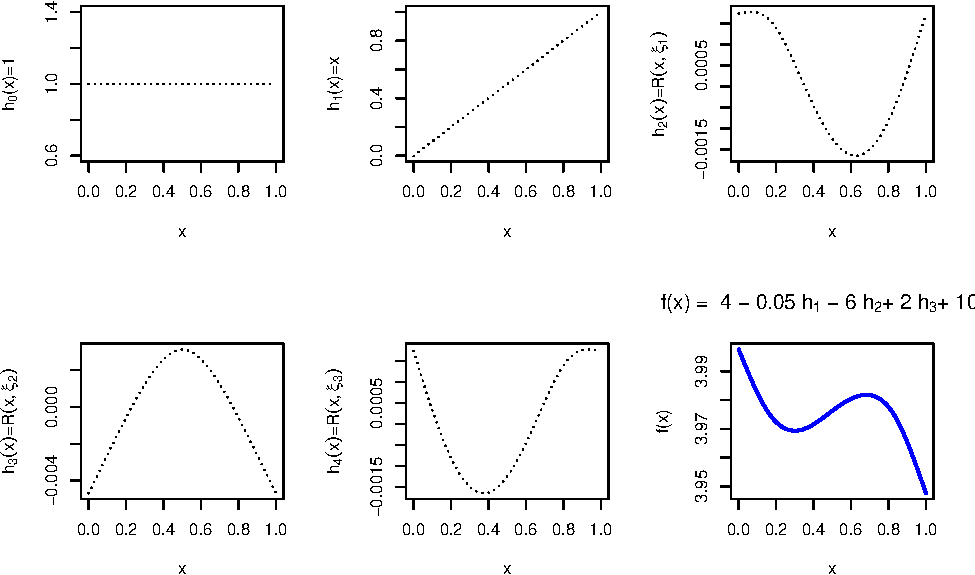
\includegraphics[keepaspectratio]{_main_files/figure-latex/unnamed-chunk-110-1.pdf}}

\subsection{\texorpdfstring{B-Splines Basis Functions in \texttt{R}}{B-Splines Basis Functions in R}}\label{b-splines-basis-functions-in-r}

In this class, one of the cubic splines basis that we are going to use is called \textbf{B-Splines}.

\textbf{Cubic B Splines Definition}

The cubic B Splines basis is defined on an interval \([a,b]\) by the following requirements on the interior basis functions with knotpoints at \(\{\xi_i\}_{i=1}^m\):

\begin{enumerate}
\def\labelenumi{\arabic{enumi}.}
\item
  A given basis function is nonzero on an interval defined by \emph{four successive knots and zero elsewhere}.
\item
  The basis function is a cubic polynomial for each subinterval between successive knots.
\item
  The basis function is continuous and is also continuous in its first and second derivatives at each knotpoint.
\item
  The basis function integrates to 1 over its support.
\item
  The boundary function definitions are adjusted to account for continuity in derivatives at the boundaries of the interval.
\end{enumerate}

These are part of the \texttt{splines} library in \texttt{R} and the function to generate then is called \texttt{bs}. The arguments of the \texttt{bs} function are:
\[ bs(x, df, knots, degree, intercept, Boundary.knots) \]
The \texttt{R} documentation can be found here.

Arguments in the \texttt{bs} function:

\begin{itemize}
\item
  \texttt{x} is the predictor, i.e.~the variable to which we want to apply the splines function.
\item
  \texttt{df} are the degrees of freedom for the splines functions.
\item
  \texttt{knots} are the \emph{internal} breakpoints/knots that define the spline, i.e.~location where the knots should be placed.
\item
  \texttt{degree} is the degree of the piecewise polynomial. The default is \texttt{degree=3} for cubic splines.
\item
  \texttt{intercept} is whether we want to add an intercept in the splines basis or not. \emph{This is not the intercept in the regression we perform}. The default is \texttt{intercept=FALSE}.
\item
  \texttt{Boundary.knots} are the boundary points at which we ``anchor'' the B-splines basis. The default values are obtained from the range of non-NA values of \texttt{x}, i.e.~\texttt{Boundary.knots=FALSE}.
\end{itemize}

So, \emph{in our examples}, we will need to feed the appropriate predictor \texttt{x} and then the desired \texttt{knots} \textbf{or} degrees of freedom, \texttt{df}, \emph{not both}. The rest we leave them at their default values.

The \textbf{output} of the \texttt{bs()} function is a \emph{matrix} of dimension \texttt{c(length(x),\ df)}, if \texttt{df} was supplied or of dimension \texttt{df\ =\ length(knots)\ +\ degree\ (+1\ if\ intercept=TRUE)} if \texttt{knots} were supplied.

\textbf{Knots or Degrees of Freedom in \texttt{bs()}}

As we mentioned, we need to supply the degrees of freedom or the location of the knots in the \texttt{bs()} function, and of course there is an equivalence between the two. Some details to keep in mind on how you can correctly specify these arguments:

\begin{itemize}
\tightlist
\item
  If you know where the knots should be placed, then you need to define a vector of the \textbf{locations} of the knots and input that in the \texttt{knots} argument in the \texttt{bs()} function. For example,
\end{itemize}

\textbf{Defining \texttt{knots} location in \texttt{bs()}}

\begin{Shaded}
\begin{Highlighting}[]
\FunctionTok{library}\NormalTok{(splines)}
\NormalTok{x}\OtherTok{=}\FunctionTok{seq}\NormalTok{(}\DecValTok{0}\NormalTok{, }\DecValTok{1}\NormalTok{, }\AttributeTok{by=}\FloatTok{0.01}\NormalTok{) }\CommentTok{\# generic \textasciigrave{}x\textasciigrave{} for illustration purposes}
\NormalTok{new.knots}\OtherTok{=} \FunctionTok{c}\NormalTok{(}\DecValTok{1}\SpecialCharTok{/}\DecValTok{6}\NormalTok{, }\DecValTok{3}\SpecialCharTok{/}\DecValTok{6}\NormalTok{, }\DecValTok{5}\SpecialCharTok{/}\DecValTok{6}\NormalTok{)  }\CommentTok{\# define three knots at locations 1/6, 3/6, 5/6.}
\NormalTok{Bsplines.basis1 }\OtherTok{=} \FunctionTok{bs}\NormalTok{(x, }\AttributeTok{knots=}\NormalTok{new.knots)}
\FunctionTok{head}\NormalTok{(Bsplines.basis1)}
\end{Highlighting}
\end{Shaded}

\begin{verbatim}
##             1         2         3 4 5 6
## [1,] 0.000000 0.0000000 0.0000000 0 0 0
## [2,] 0.165912 0.0034896 0.0000144 0 0 0
## [3,] 0.304896 0.0135168 0.0001152 0 0 0
## [4,] 0.418824 0.0294192 0.0003888 0 0 0
## [5,] 0.509568 0.0505344 0.0009216 0 0 0
## [6,] 0.579000 0.0762000 0.0018000 0 0 0
\end{verbatim}

In this case, \texttt{R} calculates the degrees of freedom using the following formula:
\[\text{df = length(knots) + degree}\]
or \textbf{if \texttt{intercept=TRUE}} then
\[\text{df = length(knots) + degree + 1}\]

\begin{itemize}
\tightlist
\item
  If you prefer to specify the degrees of freedom, then the function \texttt{bs()} chooses \texttt{df-degree} many knots at suitable quantiles of \(x\) (ignoring any missing values). If you specified \texttt{intercept=TRUE}, then the number of knots will be \texttt{df-degree-1}. For example,
\end{itemize}

\textbf{Defining \texttt{knots} location in \texttt{bs()}}

\begin{Shaded}
\begin{Highlighting}[]
\NormalTok{x}\OtherTok{=}\FunctionTok{seq}\NormalTok{(}\DecValTok{0}\NormalTok{, }\DecValTok{1}\NormalTok{, }\AttributeTok{by=}\FloatTok{0.01}\NormalTok{) }\CommentTok{\# generic \textasciigrave{}x\textasciigrave{} for illustration purposes}
\NormalTok{Bsplines.basis2 }\OtherTok{=} \FunctionTok{bs}\NormalTok{(x, }\AttributeTok{df=}\DecValTok{4}\NormalTok{)}
\FunctionTok{head}\NormalTok{(Bsplines.basis2)}
\end{Highlighting}
\end{Shaded}

\begin{verbatim}
##             1        2        3 4
## [1,] 0.000000 0.000000 0.000000 0
## [2,] 0.058214 0.000592 0.000002 0
## [3,] 0.112912 0.002336 0.000016 0
## [4,] 0.164178 0.005184 0.000054 0
## [5,] 0.212096 0.009088 0.000128 0
## [6,] 0.256750 0.014000 0.000250 0
\end{verbatim}

As an example, below we plot the first 7 B Splines basis functions:

\textbf{Illustration of B Splines Basis Function}

\begin{Shaded}
\begin{Highlighting}[]
\NormalTok{Bsplines.basis }\OtherTok{=} \FunctionTok{bs}\NormalTok{(x, }\AttributeTok{knots=}\NormalTok{new.knots)}
\FunctionTok{dim}\NormalTok{(Bsplines.basis)}
\end{Highlighting}
\end{Shaded}

\begin{verbatim}
## [1] 101   6
\end{verbatim}

\begin{Shaded}
\begin{Highlighting}[]
\FunctionTok{head}\NormalTok{(Bsplines.basis)}
\end{Highlighting}
\end{Shaded}

\begin{verbatim}
##             1         2         3 4 5 6
## [1,] 0.000000 0.0000000 0.0000000 0 0 0
## [2,] 0.165912 0.0034896 0.0000144 0 0 0
## [3,] 0.304896 0.0135168 0.0001152 0 0 0
## [4,] 0.418824 0.0294192 0.0003888 0 0 0
## [5,] 0.509568 0.0505344 0.0009216 0 0 0
## [6,] 0.579000 0.0762000 0.0018000 0 0 0
\end{verbatim}

\begin{Shaded}
\begin{Highlighting}[]
\FunctionTok{par}\NormalTok{(}\AttributeTok{mfrow =} \FunctionTok{c}\NormalTok{(}\DecValTok{2}\NormalTok{,}\DecValTok{4}\NormalTok{))}
\FunctionTok{plot}\NormalTok{(x, Bsplines.basis[,}\DecValTok{1}\NormalTok{], }\AttributeTok{type=}\StringTok{\textquotesingle{}l\textquotesingle{}}\NormalTok{, }\AttributeTok{lty=}\DecValTok{3}\NormalTok{, }\AttributeTok{ylab=}\FunctionTok{expression}\NormalTok{(}\FunctionTok{paste}\NormalTok{(h[}\DecValTok{1}\NormalTok{](x))))}
\FunctionTok{plot}\NormalTok{(x, Bsplines.basis[,}\DecValTok{2}\NormalTok{], }\AttributeTok{type=}\StringTok{\textquotesingle{}l\textquotesingle{}}\NormalTok{,}\AttributeTok{lty=}\DecValTok{3}\NormalTok{, }\AttributeTok{ylab=}\FunctionTok{expression}\NormalTok{(}\FunctionTok{paste}\NormalTok{(h[}\DecValTok{2}\NormalTok{](x))))}
\FunctionTok{plot}\NormalTok{(x, Bsplines.basis[,}\DecValTok{3}\NormalTok{], }\AttributeTok{type=}\StringTok{\textquotesingle{}l\textquotesingle{}}\NormalTok{,}\AttributeTok{lty=}\DecValTok{3}\NormalTok{, }\AttributeTok{ylab=}\FunctionTok{expression}\NormalTok{(}\FunctionTok{paste}\NormalTok{(h[}\DecValTok{3}\NormalTok{](x)) ))}
\FunctionTok{plot}\NormalTok{(x, Bsplines.basis[,}\DecValTok{4}\NormalTok{], }\AttributeTok{type=}\StringTok{\textquotesingle{}l\textquotesingle{}}\NormalTok{,}\AttributeTok{lty=}\DecValTok{3}\NormalTok{, }\AttributeTok{ylab=}\FunctionTok{expression}\NormalTok{(}\FunctionTok{paste}\NormalTok{(h[}\DecValTok{4}\NormalTok{](x))))}
\FunctionTok{plot}\NormalTok{(x, Bsplines.basis[,}\DecValTok{5}\NormalTok{], }\AttributeTok{type=}\StringTok{\textquotesingle{}l\textquotesingle{}}\NormalTok{,}\AttributeTok{lty=}\DecValTok{3}\NormalTok{, }\AttributeTok{ylab=}\FunctionTok{expression}\NormalTok{(}\FunctionTok{paste}\NormalTok{(h[}\DecValTok{5}\NormalTok{](x))))}
\FunctionTok{plot}\NormalTok{(x, Bsplines.basis[,}\DecValTok{6}\NormalTok{], }\AttributeTok{type=}\StringTok{\textquotesingle{}l\textquotesingle{}}\NormalTok{,}\AttributeTok{lty=}\DecValTok{3}\NormalTok{, }\AttributeTok{ylab=}\FunctionTok{expression}\NormalTok{(}\FunctionTok{paste}\NormalTok{(h[}\DecValTok{6}\NormalTok{](x))))}
\end{Highlighting}
\end{Shaded}

\pandocbounded{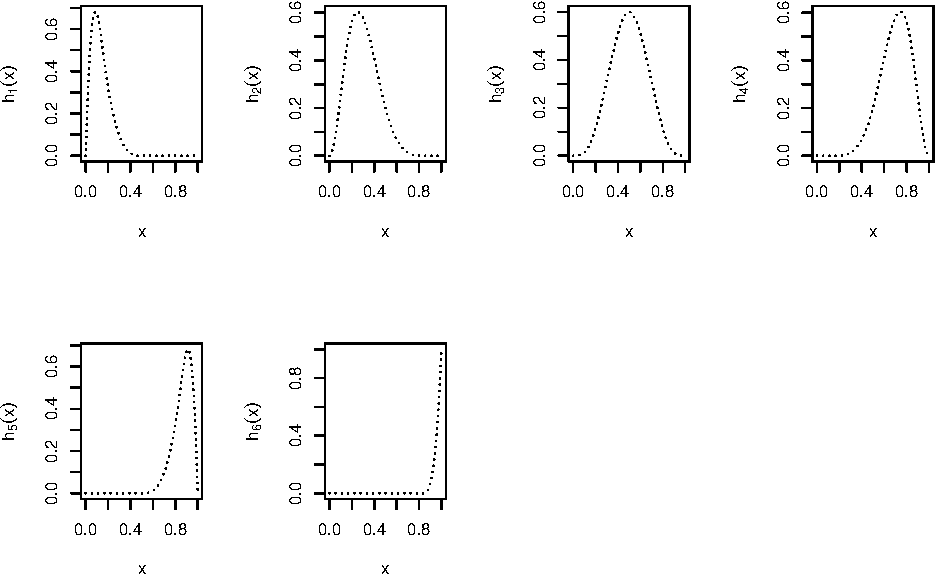
\includegraphics[keepaspectratio]{_main_files/figure-latex/unnamed-chunk-114-1.pdf}}

\subsection{Natural Cubic Splines (NCS)}\label{natural-cubic-splines-ncs}

A cubic spline on \([a, b]\) is a \textbf{Natural Cubic Spline} if its \emph{second} and \emph{third} derivatives are \emph{zero at \(a\) and \(b\)}. This condition implies that NCS is a linear function in the two extreme intervals \([a,\xi_1]\) and \([\xi_m,b]\). The linear functions in the two extreme intervals are completely determined by their neighboring intervals. The degrees of freedom of NCS's with \(m\) knots are:
\[4(m+1)-3m -4=m\]
since we have 4 additional constraints (the ones on the boundary points).

\textbf{Remark}: For a curve estimation problem with data \((x_i,y_i)^n_{i=1}\), if we put \(n\) knots at the \(n\) data points (assumed to be unique), then using NCS we obtain a \emph{smooth} curve passing through \textbf{all} \(y\)'s.

\textbf{Natural Cubic Spline}

A Natural Cubic Spline with \(m\) knots is represented by \(m\) basis functions, for example one such basis is given by
\begin{align*}
 N_1(x) &= 1\\
 N_2(x) &= x\\
 N_{k+2} (x) &= d_k(x) - d_{k-1}(x)
 \end{align*}
where
\[d_k(x) = \frac{(x-\xi_k)_{+}^{3} - (x-\xi_{m})_{+}^{3}}{\xi_m - \xi_k}\]
Each of these derivatives can be seen to have zero second and third derivative for \(x\geq \xi_m\).

In \texttt{R} we can find the NCS as part of the \texttt{splines} library, by calling the \texttt{ns()} function. Specifically, we have that

\[ ns(x, df, knots, intercept=TRUE, Boundary.knots) \]

\textbf{Natural Cubic Splines in \texttt{R}}

\begin{Shaded}
\begin{Highlighting}[]
\NormalTok{NCS.basis }\OtherTok{=}\FunctionTok{ns}\NormalTok{(x, }\AttributeTok{knots=}\NormalTok{new.knots, }\AttributeTok{Boundary.knots=}\FunctionTok{c}\NormalTok{(}\DecValTok{0}\NormalTok{,}\DecValTok{1}\NormalTok{))}
\FunctionTok{dim}\NormalTok{(NCS.basis)}
\end{Highlighting}
\end{Shaded}

\begin{verbatim}
## [1] 101   4
\end{verbatim}

\begin{Shaded}
\begin{Highlighting}[]
\FunctionTok{par}\NormalTok{(}\AttributeTok{mfrow =} \FunctionTok{c}\NormalTok{(}\DecValTok{2}\NormalTok{,}\DecValTok{3}\NormalTok{))}
\FunctionTok{plot}\NormalTok{(x, NCS.basis[,}\DecValTok{1}\NormalTok{], }\AttributeTok{type=}\StringTok{\textquotesingle{}l\textquotesingle{}}\NormalTok{, }\AttributeTok{lty=}\DecValTok{3}\NormalTok{, }\AttributeTok{ylab=}\FunctionTok{expression}\NormalTok{(}\FunctionTok{paste}\NormalTok{(h[}\DecValTok{1}\NormalTok{](x))))}
\FunctionTok{plot}\NormalTok{(x, NCS.basis[,}\DecValTok{2}\NormalTok{], }\AttributeTok{type=}\StringTok{\textquotesingle{}l\textquotesingle{}}\NormalTok{,}\AttributeTok{lty=}\DecValTok{3}\NormalTok{, }\AttributeTok{ylab=}\FunctionTok{expression}\NormalTok{(}\FunctionTok{paste}\NormalTok{(h[}\DecValTok{2}\NormalTok{](x))))}
\FunctionTok{plot}\NormalTok{(x, NCS.basis[,}\DecValTok{3}\NormalTok{], }\AttributeTok{type=}\StringTok{\textquotesingle{}l\textquotesingle{}}\NormalTok{,}\AttributeTok{lty=}\DecValTok{3}\NormalTok{, }\AttributeTok{ylab=}\FunctionTok{expression}\NormalTok{(}\FunctionTok{paste}\NormalTok{(h[}\DecValTok{3}\NormalTok{](x)) ))}
\FunctionTok{plot}\NormalTok{(x, NCS.basis[,}\DecValTok{4}\NormalTok{], }\AttributeTok{type=}\StringTok{\textquotesingle{}l\textquotesingle{}}\NormalTok{,}\AttributeTok{lty=}\DecValTok{3}\NormalTok{, }\AttributeTok{ylab=}\FunctionTok{expression}\NormalTok{(}\FunctionTok{paste}\NormalTok{(h[}\DecValTok{4}\NormalTok{](x))))}
\end{Highlighting}
\end{Shaded}

\pandocbounded{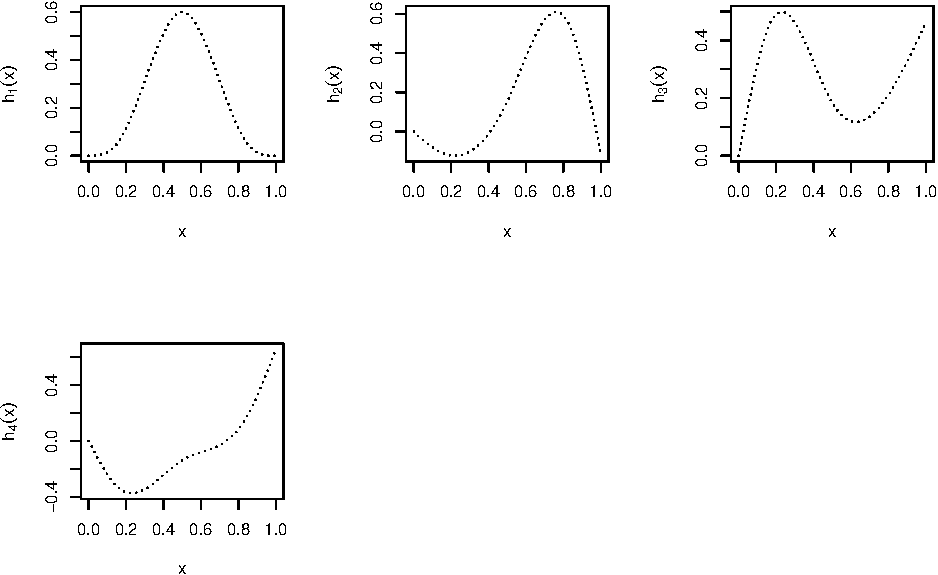
\includegraphics[keepaspectratio]{_main_files/figure-latex/unnamed-chunk-115-1.pdf}}

Recall that the linear functions in the two extreme intervals are completely determined by the other cubic splines. This means that data points in the two extreme intervals (i.e., outside the two boundary knots) are wasted since they do not affect the fitting. Therefore, by default, \texttt{R} puts the two boundary knots as the \emph{min} and \emph{max} of the \(x_i\)'s.

As in the case of the \texttt{bs()} function:

\begin{itemize}
\item
  You can tell \texttt{R} the location of knots, which are the interior knots. Recall that a NCS with \(m\) knots has \(m\) df. So, the df is equal to the number of (interior) knots plus \(2\), where \(2\) means the two boundary knots.
\item
  Or you can tell \texttt{R} the df. If intercept = TRUE, then we need \(m= df - 2\) knots, otherwise we need \(m = df - 1\) knots. Again, by default, \texttt{R} puts knots at the \(1/(m+1),...,m/(m+1)\) quantiles of \(x_{1:n}\).
\end{itemize}

\subsection{Regression Splines}\label{regression-splines}

Recall that for a given set of knots, the corresponding cubic splines form a \emph{linear space} of functions with dimension \((m + 4)\). So, the \textbf{Regression Splines} use a basis expansion approach:
\[g(x)=\beta_1 h_1(x)+\beta_2 h_2(x)+\ldots+\beta_p h_p(x)\]
* If Cubic Splines are used as basis functions \(p=m+4\).

\begin{itemize}
\tightlist
\item
  If Natural Cubic Splines (NCS) are used as basis functions \(p=m\).
\end{itemize}

We can represent the model on the observed \(n\) data points using matrix notation:
\[
      \begin{pmatrix}
        y_1\\
        y_2\\
        \ldots\\
        y_n
      \end{pmatrix}_{n\times 1} =
      \begin{pmatrix}
         h_1(x_1)& \ldots & h_{p}(x_1)\\
          h_1(x_2)& \ldots & h_{p}(x_2)\\
         \\
           h_1(x_n)& \ldots & h_{p}(x_n)
      \end{pmatrix}_{n\times p}
      \begin{pmatrix}
      \beta_1\\
      \beta_2\\
      \ldots\\
      \beta_p
      \end{pmatrix}_{p\times 1}
\]
where our \emph{``design''} matrix is the matrix \(\mathbf{F}\) of basis functions. Therefore, we can estimate the coefficients \(\mathbf{\beta}\) by solving the following Least-Squares problem:
\[\hat{\mathbf{\beta}}= \arg\min_{\mathbf{\beta}}||\mathbf{y} - \mathbf{F}{\mathbf{\beta}|}|^2\]

\subsection{K-Fold Cross-Validation}\label{k-fold-cross-validation}

One of the challenges in using splines regression is the choice of the degrees of freedom/ knots. One way to optimally select the number of knots or degrees of freedom is the so-called K-fold cross-validation approach. This is outlined in the steps below:

\begin{enumerate}
\def\labelenumi{\arabic{enumi}.}
\tightlist
\item
  Set a fixed number of knots (or df).
\item
  Divide the set of observations into \(k\) groups (or \emph{folds}).
\item
  Leave the first fold as a validation set (not used to fit the model). Fit the Regression Spline with a fixed number of knots using the remaining \(k-1\) folds.
\item
  Calculate the Mean Square Error for fold 1: \(MSE_1\).
\item
  Repeat the previous steps \(k\) times. Each time a new validation set is used to calculate \(MSE_i\).
\item
  Calculate the average \(k\)-fold Cross-Validation error: \[CV(k)=\frac{1}{k}\sum_{i=1}^k MSE_i\]
\item
  Repeat 2 to 6 with a new number of knots (or df).
\item
  Select the number of knots that minimizes the \(k\)-fold CV error or \(CV(k)\).
\end{enumerate}

Then, we repeat the same process for a different number of knots and in the end we select the one that minimizes the \(CV(k)\). A sketch of this approach is shown below:

\begin{center}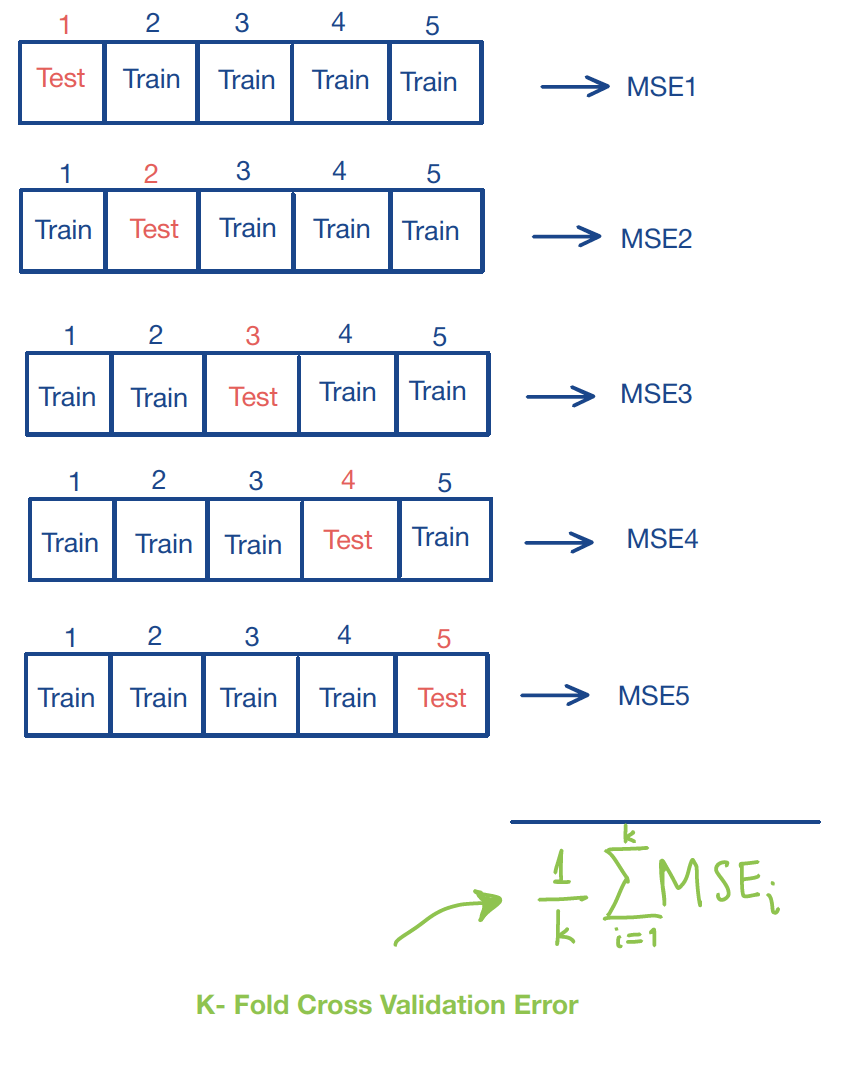
\includegraphics[width=0.6\linewidth]{images/week4/kfold} \end{center}

\section{Smoothing Splines}\label{smoothing-splines}

In Regression Splines, we need to choose the number and the location of knots (or the degrees of freedom). As we discussed, B-splines and NCS are both methods that construct a \(n \times p\) basis matrix \(\mathbf{F}\), and then model the outcome using a linear regression on \(\mathbf{F}\). Inevitably, we need to select the order of the spline, the number of knots (AIC, BIC, CV) and even the location of knots, which is a quite challenging task. So, we need to consider whether there is an alternative approach that we can use to select the number and location of knots automatically.

A Smoothing Spline is a spline designed to balance fit with smoothness, and it starts by suggesting a very bad solution to our problem: by putting knots at \textit{all} the observed data points \((x_1, \ldots, x_n)\):
\[\mathbf{y}_{n\times 1} = \mathbf{F}_{n\times p} \beta_{p\times 1}\]
Then, we can construct \(n\) NCS basis. However, we know that with this approach we are going to run into overfitting problems. So, instead of selecting the knots, we recall last week's discussion on penalizing models with many parameters. This leads to minimizing the following objective functions with a ridge-type shrinkage:
\[\min_{\beta} \Bigl\{ ||\mathbf{y}-\mathbf{F} \beta ||^2 + \lambda \beta^T \Omega \beta \Bigr\}\]
where the tuning parameter \(\lambda\) is often chosen by CV (\(\Omega\) will be defined later).

So, now we want to understand whether solving such a minimzation problem can provide us with a good solution with desirable properties.

\subsection{The Roughness Penalty Approach}\label{the-roughness-penalty-approach}

Let \(S[a,b]\) be the space of all ``smooth'\,' functions defined on \([a,b]\). This is a second order Sobolev space where global polynomial functions and cubic splines functions live (\(S[a,b]\) is an infinite-dimensional function space. Our goal is to find the best function in \(S[a,b]\) to approximate \(f\).

Let us consider solving the following Penalized Residual Sum of Squares problem:
\[
RSS_\lambda(g) = \sum_{i=1}^n [y_i - g(x_i)]^2  + \lambda \int_a^b [g''(x)]^2 dx.
\]
where \(\lambda\) is a smoothing parameter. The first term measures the closeness of the model to the data, while the second term penalizes the roughness/curvature of the function. We solve this problem on \([a,b]=[\min x_i, \max _i]\) for functions with finite roughness penalty \(\int_a^b [g''(x)]^2 dx < \infty\). This is known as a second order Sobolev space.

Note that \(\int_a^b [g''(x)]^2 dx\) is called the \textbf{roughness penalty}.

From the expression above, we can see that \(\lambda\) is the smoothing parameter that controls the bias-variance trade-off. Therefore, when \(\lambda=0\), we interpolate the data and that leads us to overfitting. When \(\lambda=\infty\), then we return to linear least-squares regression. It turns out that the solution to the penalized residual sum of squares has to be a NCS. Indeed,

\textbf{Theorem}
\[\min_g RSS_{\lambda}(g) = \min_{\tilde{g}} RSS_{\lambda}(\tilde{g}) \]\}
where \(\tilde{g}\) is a NCS with knots at the \(n\) data points.

Let's call \(g(x)\) the as the optimal solution. Since the loss part in \(RSS_\lambda(g)\) only involves \(n\) data points, we can find define a natural cubic spline (NCS) fit that we can call \(\tilde{g}(x)\) such that it matches \(g(x)\) at the observations \(x_i\), \(i=1, \ldots, n\), i.e.
\[g(x_i) = \tilde{g}(x_i), i=1, \ldots, n\]
We can always find such \(\tilde{g}\) since our space consists of \(n\) basis. Then, we can show that
\[\int g^{''2} dx \geq \int  \tilde{g}^{''2} dx\]
meaning that we will \emph{always} prefer the \(\tilde{g}\), the NCS ``representation'\,' of
\(g\), since the \emph{penalty} is smaller, and the \emph{loss} doesn't change.

\subsection{Proof}\label{proof}

To establish the Theorem, we essentially need to show that
\[\int g''^{2} dx \geq \int  \tilde{g}''^{2} dx\]

Thus, we define \(h(x) = g(x) - \tilde{g}(x)\) for which we know that \(h(x_i)=0\) for \(i=1, \ldots, n\). Then
\[ \int g''^2 \, dx  = \int \tilde{g}''^2 \, dx  + \int h''^2 \, dx  + 2 \int \tilde{g}'' h'' \, dx
\]
and without loss of generality assuming that the \(x_i\)s are ordered, we obtain:
\begin{align*}
\int \tilde{g}'' h'' \, dx  &= \tilde{g}'' h' \Big|_a^b 
- \int_a^b h' \tilde{g}^{(3)} \, dx\\
&= - \sum_{i=1}^{n-1} \tilde{g}^{(3)}\!\left(x_j^+\right) 
\int_{x_j}^{x_{j+1}} h' \, dx 
\quad (\tilde{g}^{(3)} \text{ constant piecewise})\\
&= - \sum_{i=1}^{n-1} \tilde{g}^{(3)}\!\left(x_j^+\right) 
\left(h(x_{j+1}) - h(x_j)\right)
\end{align*}
The second equation is because \(\tilde{g}\) is a NCS and therefore we know that it has zero second derivative on the two boundaries \(a\) and \(b\). The third equation is true, because \(\tilde{g}\) is at most a 3rd order polynomial on any region and as a consequence has constant third derivatives, which we can pull out of the integration. The last equation holds because we said that \(h(x)=0\) on all the observation points \(x_i\). Therefore, this shows that the roughness penalty of our NCS solution is no larger than the best solution \(g\). If we also take into account that \(\tilde{g}\) is also in the space \(S[a,b]\), then \(g\) must be our NCS solution.

\section{Fitting Smoothing Splines}\label{fitting-smoothing-splines}

From the previous discussion, we conclude that \(g\) has a \textbf{finite sample representation}
\[\hat{g}(x) = \sum_i \beta_i N_i(x)\]
where \(N_i\) are a set of NCS basis functions with knots at each of the \(x\) \emph{unique} values. Therefore, the penalty function becomes
\begin{align*}
\int_{a}^{b} g^{''2} dx &= \int  \left( \sum_i \beta_i N_i^{''}(x)\right)^2 dx\\
&= \sum_{i,j} \beta_i \beta_j \int N_i^{''}(x) N_j^{''}(x) dx\\
&=\beta^T \Omega \beta
\end{align*}
where \(\Omega_{n\times n}\) with \(\Omega_{ij} = \int N^{''}_{i}(x) N^{''}_{j}(x) dx\).

Hence our goal is to find \(\beta\) that minimizes
\[RSS_{\lambda}(\beta) = (\mathbf{y} - \mathbf{F}\beta)^T(\mathbf{y} - \mathbf{F}\beta) + \lambda  \beta^T \Omega \beta \]
This is a ridge penalized function and the solution is
\[\hat{\beta} = \arg \min_{\beta} RSS_{\lambda}(\beta)\]
\[=(\mathbf{F}^T \mathbf{F} +\lambda \Omega)^{-1} \mathbf{F}^T \mathbf{y}\]

The smoothing spline version of the ``hat'\,' matrix is called the \textbf{smoother matrix}
\[\mathbf{\hat{y}} = \mathbf{F} (\mathbf{F}^T \mathbf{F} +\lambda \Omega)^{-1} \mathbf{F}^T \mathbf{y} = S_{\lambda} \mathbf{y}\]

\textbf{Remarks}

We have done the analysis of degrees of freedom for ridge type regression. The degrees of freedom of a smoothing spline are
\[df = tr(S_{\lambda})\]
which ranges between 0 and \(n\). Under some special constructions (Demmler and Reinsch,
1975), a basis with double orthogonality property, can lead to
\[\mathbf{F}^T \mathbf{F} = \mathbf{I}, \Omega = diag(d_i)\]
where \(d_i\)s are arranges in an increasing order and in addition \(d_2=d_1=0\). Using this basis we have
\[\hat{\beta} = (\mathbf{F}^T \mathbf{F} +\lambda \Omega)^{-1} \mathbf{F}^T \mathbf{y} = \Bigl(\mathbf{I} + \lambda diag(d_i) \Bigr)^{-1} \mathbf{F}^T \mathbf{y}\]
i.e.
\[\hat{\beta}_i = \frac{1}{1+\lambda d_i} \hat{\beta}_i^{LS}\]

\textbf{Choosing \(\lambda\)}

Choosing the penalty \(\lambda\) is the same as in ridge regression.

-- Leave-one-out CV:
\[
  \text{CV}(\lambda) = \frac{1}{n} \sum_{i=1}^n \left( \frac{y_i - \hat g(x_i)}{1 - S_\lambda(i,i)} \right)^2.
  \]

-- Generalized CV:
\[
  \text{GCV}(\lambda) = \frac{1}{n} \sum_{i=1}^n \left( \frac{y_i - \hat g(x_i)}{1 - \tfrac{1}{n}\text{tr}(S_\lambda)} \right)^2.
  \]

\section{\texorpdfstring{The \texttt{Birthrates} Example in R}{The Birthrates Example in R}}\label{the-birthrates-example-in-r}

The Birthrate data set contains U.S. birth rate data from 1917 to 2003.

\begin{Shaded}
\begin{Highlighting}[]
\NormalTok{birthrates}\OtherTok{=} \FunctionTok{read.csv}\NormalTok{(}\StringTok{"data/week4/birthrates.csv"}\NormalTok{)}
\FunctionTok{head}\NormalTok{(birthrates)}
\end{Highlighting}
\end{Shaded}

\begin{verbatim}
##   Year Birthrate
## 1 1917     183.1
## 2 1918     183.9
## 3 1919     163.1
## 4 1920     179.5
## 5 1921     181.4
## 6 1922     173.4
\end{verbatim}

Plotting the data we have

\begin{Shaded}
\begin{Highlighting}[]
\FunctionTok{plot}\NormalTok{(birthrates, }\AttributeTok{pch =} \DecValTok{19}\NormalTok{, }\AttributeTok{col =} \StringTok{"blue"}\NormalTok{)}
\end{Highlighting}
\end{Shaded}

\pandocbounded{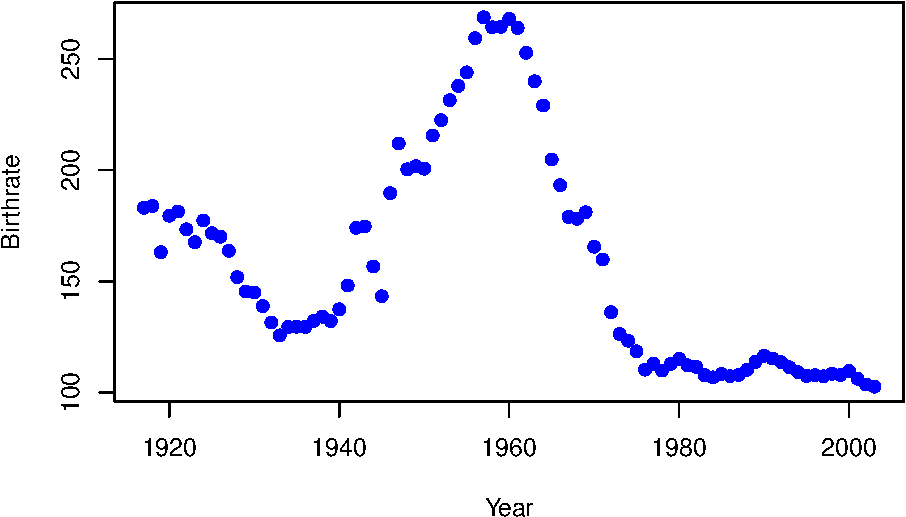
\includegraphics[keepaspectratio]{_main_files/figure-latex/unnamed-chunk-118-1.pdf}}

which is an highly nonlinear trend.

We first try to fit a polynomial regression with orthogonal polynomials for polynomials with degrees 3, and 6. The fitted lines can be shown below:

\begin{Shaded}
\begin{Highlighting}[]
\FunctionTok{par}\NormalTok{(}\AttributeTok{mfrow=}\FunctionTok{c}\NormalTok{(}\DecValTok{1}\NormalTok{,}\DecValTok{2}\NormalTok{))}

\NormalTok{    poly3.fit }\OtherTok{\textless{}{-}} \FunctionTok{lm}\NormalTok{(Birthrate }\SpecialCharTok{\textasciitilde{}} \FunctionTok{poly}\NormalTok{(Year, }\DecValTok{3}\NormalTok{), }\AttributeTok{data =}\NormalTok{ birthrates)}
    \FunctionTok{plot}\NormalTok{(birthrates, }\AttributeTok{pch =} \DecValTok{19}\NormalTok{, }\AttributeTok{col =} \StringTok{"blue"}\NormalTok{)}
    \FunctionTok{lines}\NormalTok{(birthrates}\SpecialCharTok{$}\NormalTok{Year, poly3.fit}\SpecialCharTok{$}\NormalTok{fitted.values, }\AttributeTok{lty =} \DecValTok{1}\NormalTok{, }\AttributeTok{col =} \StringTok{"magenta"}\NormalTok{, }\AttributeTok{lwd =} \DecValTok{2}\NormalTok{)}
    \FunctionTok{title}\NormalTok{(}\StringTok{"degree = 3"}\NormalTok{)}
    
    \FunctionTok{par}\NormalTok{(}\AttributeTok{mar =} \FunctionTok{c}\NormalTok{(}\DecValTok{2}\NormalTok{,}\DecValTok{3}\NormalTok{,}\DecValTok{2}\NormalTok{,}\DecValTok{0}\NormalTok{))}
\NormalTok{    poly6.fit }\OtherTok{\textless{}{-}} \FunctionTok{lm}\NormalTok{(Birthrate }\SpecialCharTok{\textasciitilde{}} \FunctionTok{poly}\NormalTok{(Year, }\DecValTok{6}\NormalTok{), }\AttributeTok{data =}\NormalTok{ birthrates)}
    \FunctionTok{plot}\NormalTok{(birthrates, }\AttributeTok{pch =} \DecValTok{19}\NormalTok{, }\AttributeTok{col =} \StringTok{"blue"}\NormalTok{)}
    \FunctionTok{lines}\NormalTok{(birthrates}\SpecialCharTok{$}\NormalTok{Year, poly6.fit}\SpecialCharTok{$}\NormalTok{fitted.values, }\AttributeTok{lty =} \DecValTok{1}\NormalTok{, }\AttributeTok{col =} \StringTok{"magenta"}\NormalTok{, }\AttributeTok{lwd =} \DecValTok{2}\NormalTok{)}
    \FunctionTok{title}\NormalTok{(}\StringTok{"degree = 6"}\NormalTok{)}
\end{Highlighting}
\end{Shaded}

\pandocbounded{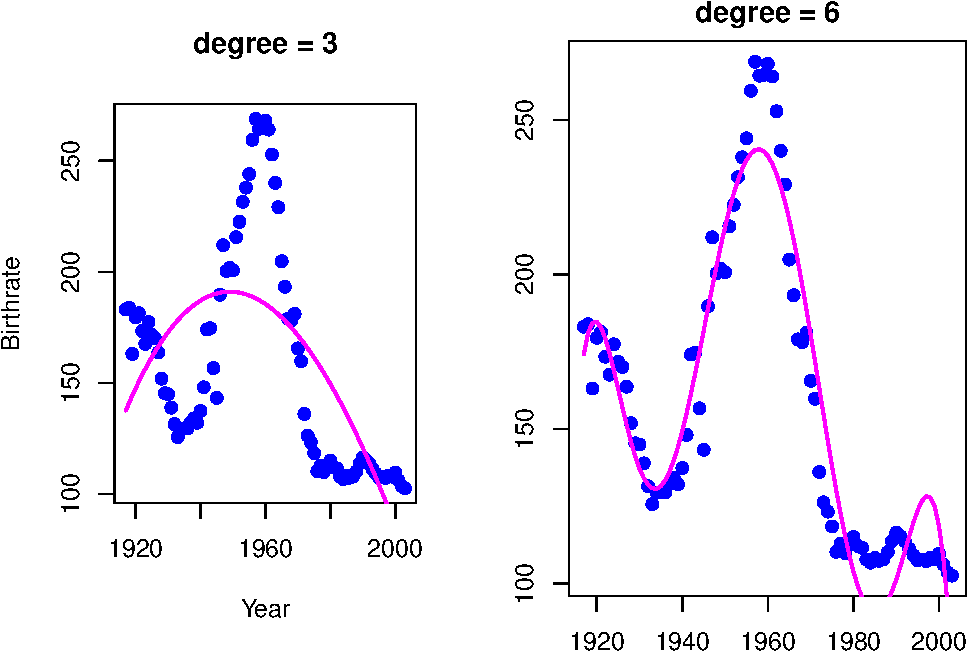
\includegraphics[keepaspectratio]{_main_files/figure-latex/unnamed-chunk-119-1.pdf}}

We can see that the 6th order polynomial is better, but it is not very good. We can try fitting local polynomials - piecewise polynomials of lower order (we try constant functions and linear function in the example below:

\begin{Shaded}
\begin{Highlighting}[]
\NormalTok{ myknots }\OtherTok{=} \FunctionTok{c}\NormalTok{(}\DecValTok{1936}\NormalTok{, }\DecValTok{1960}\NormalTok{, }\DecValTok{1978}\NormalTok{)}

\NormalTok{ bounds }\OtherTok{=} \FunctionTok{c}\NormalTok{(}\DecValTok{1917}\NormalTok{, myknots, }\DecValTok{2003}\NormalTok{)  }
    
 \CommentTok{\# Piecewise Constant Polynomials}
\NormalTok{    mybasis }\OtherTok{=} \FunctionTok{cbind}\NormalTok{(}\StringTok{"x\_1"} \OtherTok{=}\NormalTok{ (birthrates}\SpecialCharTok{$}\NormalTok{Year }\SpecialCharTok{\textless{}}\NormalTok{ myknots[}\DecValTok{1}\NormalTok{]), }
                    \StringTok{"x\_2"} \OtherTok{=}\NormalTok{ (birthrates}\SpecialCharTok{$}\NormalTok{Year }\SpecialCharTok{\textgreater{}=}\NormalTok{ myknots[}\DecValTok{1}\NormalTok{])}\SpecialCharTok{*}\NormalTok{(birthrates}\SpecialCharTok{$}\NormalTok{Year }\SpecialCharTok{\textless{}}\NormalTok{ myknots[}\DecValTok{2}\NormalTok{]), }
                    \StringTok{"x\_3"} \OtherTok{=}\NormalTok{ (birthrates}\SpecialCharTok{$}\NormalTok{Year }\SpecialCharTok{\textgreater{}=}\NormalTok{ myknots[}\DecValTok{2}\NormalTok{])}\SpecialCharTok{*}\NormalTok{(birthrates}\SpecialCharTok{$}\NormalTok{Year }\SpecialCharTok{\textless{}}\NormalTok{ myknots[}\DecValTok{3}\NormalTok{]),}
                    \StringTok{"x\_4"} \OtherTok{=}\NormalTok{ (birthrates}\SpecialCharTok{$}\NormalTok{Year }\SpecialCharTok{\textgreater{}=}\NormalTok{ myknots[}\DecValTok{3}\NormalTok{]))}
        
\NormalTok{    const.fit }\OtherTok{\textless{}{-}} \FunctionTok{lm}\NormalTok{(birthrates}\SpecialCharTok{$}\NormalTok{Birthrate }\SpecialCharTok{\textasciitilde{}}\NormalTok{ . }\SpecialCharTok{{-}}\DecValTok{1}\NormalTok{, }\AttributeTok{data =} \FunctionTok{data.frame}\NormalTok{(mybasis))}
    \FunctionTok{par}\NormalTok{(}\AttributeTok{mar =} \FunctionTok{c}\NormalTok{(}\DecValTok{2}\NormalTok{,}\DecValTok{3}\NormalTok{,}\DecValTok{2}\NormalTok{,}\DecValTok{0}\NormalTok{))    }
    \FunctionTok{plot}\NormalTok{(birthrates, }\AttributeTok{pch =} \DecValTok{19}\NormalTok{, }\AttributeTok{col =} \StringTok{"blue"}\NormalTok{)}
    \FunctionTok{abline}\NormalTok{(}\AttributeTok{v =}\NormalTok{ myknots, }\AttributeTok{lty =} \DecValTok{2}\NormalTok{)}
    \FunctionTok{title}\NormalTok{(}\StringTok{"Piecewise constant"}\NormalTok{)}
    
    \ControlFlowTok{for}\NormalTok{ (k }\ControlFlowTok{in} \DecValTok{1}\SpecialCharTok{:}\DecValTok{4}\NormalTok{)}
        \FunctionTok{points}\NormalTok{(}\FunctionTok{c}\NormalTok{(bounds[k], bounds[k}\SpecialCharTok{+}\DecValTok{1}\NormalTok{]), }\FunctionTok{rep}\NormalTok{(const.fit}\SpecialCharTok{$}\NormalTok{coefficients[k], }\DecValTok{2}\NormalTok{), }\AttributeTok{type =} \StringTok{"l"}\NormalTok{, }\AttributeTok{lty =} \DecValTok{1}\NormalTok{, }\AttributeTok{col =} \StringTok{"magenta"}\NormalTok{, }\AttributeTok{lwd =} \DecValTok{4}\NormalTok{)}
\end{Highlighting}
\end{Shaded}

\pandocbounded{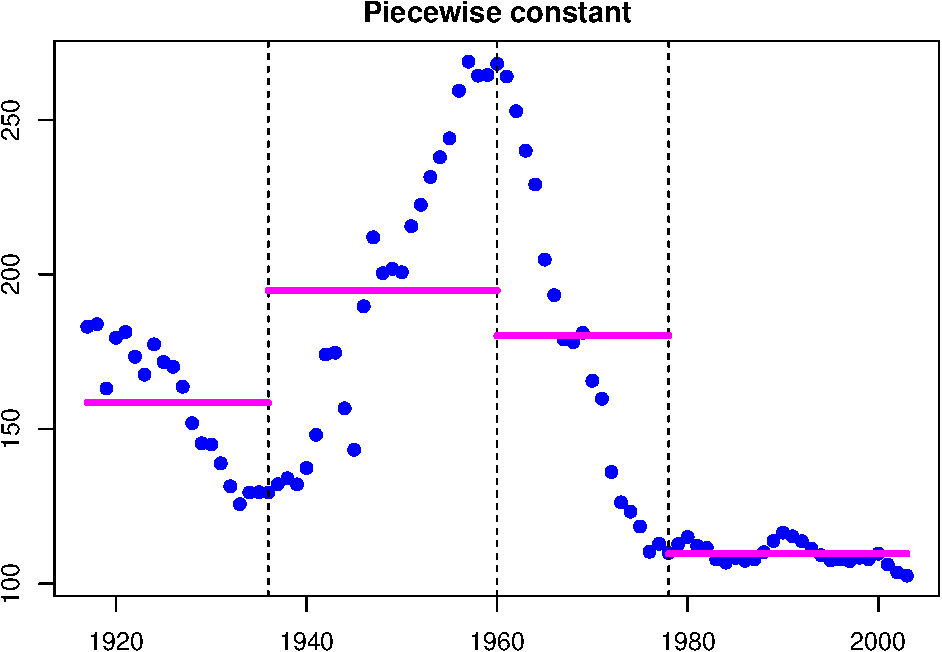
\includegraphics[keepaspectratio]{_main_files/figure-latex/unnamed-chunk-120-1.pdf}}

\begin{Shaded}
\begin{Highlighting}[]
    \CommentTok{\# Piecewise Linear Polynomials}
\NormalTok{    mybasis }\OtherTok{=} \FunctionTok{cbind}\NormalTok{(}\StringTok{"x\_1"} \OtherTok{=}\NormalTok{ (birthrates}\SpecialCharTok{$}\NormalTok{Year }\SpecialCharTok{\textless{}}\NormalTok{ myknots[}\DecValTok{1}\NormalTok{]), }
                    \StringTok{"x\_2"} \OtherTok{=}\NormalTok{ (birthrates}\SpecialCharTok{$}\NormalTok{Year }\SpecialCharTok{\textgreater{}=}\NormalTok{ myknots[}\DecValTok{1}\NormalTok{])}\SpecialCharTok{*}\NormalTok{(birthrates}\SpecialCharTok{$}\NormalTok{Year }\SpecialCharTok{\textless{}}\NormalTok{ myknots[}\DecValTok{2}\NormalTok{]), }
                    \StringTok{"x\_3"} \OtherTok{=}\NormalTok{ (birthrates}\SpecialCharTok{$}\NormalTok{Year }\SpecialCharTok{\textgreater{}=}\NormalTok{ myknots[}\DecValTok{2}\NormalTok{])}\SpecialCharTok{*}\NormalTok{(birthrates}\SpecialCharTok{$}\NormalTok{Year }\SpecialCharTok{\textless{}}\NormalTok{ myknots[}\DecValTok{3}\NormalTok{]),}
                    \StringTok{"x\_4"} \OtherTok{=}\NormalTok{ (birthrates}\SpecialCharTok{$}\NormalTok{Year }\SpecialCharTok{\textgreater{}=}\NormalTok{ myknots[}\DecValTok{3}\NormalTok{]),}
                    \StringTok{"x\_11"} \OtherTok{=}\NormalTok{ birthrates}\SpecialCharTok{$}\NormalTok{Year}\SpecialCharTok{*}\NormalTok{(birthrates}\SpecialCharTok{$}\NormalTok{Year }\SpecialCharTok{\textless{}}\NormalTok{ myknots[}\DecValTok{1}\NormalTok{]), }
                    \StringTok{"x\_21"} \OtherTok{=}\NormalTok{ birthrates}\SpecialCharTok{$}\NormalTok{Year}\SpecialCharTok{*}\NormalTok{(birthrates}\SpecialCharTok{$}\NormalTok{Year }\SpecialCharTok{\textgreater{}=}\NormalTok{ myknots[}\DecValTok{1}\NormalTok{])}\SpecialCharTok{*}\NormalTok{(birthrates}\SpecialCharTok{$}\NormalTok{Year }\SpecialCharTok{\textless{}}\NormalTok{ myknots[}\DecValTok{2}\NormalTok{]), }
                    \StringTok{"x\_31"} \OtherTok{=}\NormalTok{ birthrates}\SpecialCharTok{$}\NormalTok{Year}\SpecialCharTok{*}\NormalTok{(birthrates}\SpecialCharTok{$}\NormalTok{Year }\SpecialCharTok{\textgreater{}=}\NormalTok{ myknots[}\DecValTok{2}\NormalTok{])}\SpecialCharTok{*}\NormalTok{(birthrates}\SpecialCharTok{$}\NormalTok{Year }\SpecialCharTok{\textless{}}\NormalTok{ myknots[}\DecValTok{3}\NormalTok{]),}
                    \StringTok{"x\_41"} \OtherTok{=}\NormalTok{ birthrates}\SpecialCharTok{$}\NormalTok{Year}\SpecialCharTok{*}\NormalTok{(birthrates}\SpecialCharTok{$}\NormalTok{Year }\SpecialCharTok{\textgreater{}=}\NormalTok{ myknots[}\DecValTok{3}\NormalTok{]))}
        
\NormalTok{    line.fit }\OtherTok{\textless{}{-}} \FunctionTok{lm}\NormalTok{(birthrates}\SpecialCharTok{$}\NormalTok{Birthrate }\SpecialCharTok{\textasciitilde{}}\NormalTok{ .}\SpecialCharTok{{-}}\DecValTok{1}\NormalTok{, }\AttributeTok{data =} \FunctionTok{data.frame}\NormalTok{(mybasis))}
    \FunctionTok{par}\NormalTok{(}\AttributeTok{mar =} \FunctionTok{c}\NormalTok{(}\DecValTok{2}\NormalTok{,}\DecValTok{3}\NormalTok{,}\DecValTok{2}\NormalTok{,}\DecValTok{0}\NormalTok{))  }
    \FunctionTok{plot}\NormalTok{(birthrates, }\AttributeTok{pch =} \DecValTok{19}\NormalTok{, }\AttributeTok{col =} \StringTok{"blue"}\NormalTok{)}
    \FunctionTok{abline}\NormalTok{(}\AttributeTok{v =}\NormalTok{ myknots, }\AttributeTok{lty =} \DecValTok{2}\NormalTok{)}
    \FunctionTok{title}\NormalTok{(}\StringTok{"Piecewise linear"}\NormalTok{)}
    
    \ControlFlowTok{for}\NormalTok{ (k }\ControlFlowTok{in} \DecValTok{1}\SpecialCharTok{:}\DecValTok{4}\NormalTok{)}
        \FunctionTok{points}\NormalTok{(}\FunctionTok{c}\NormalTok{(bounds[k], bounds[k}\SpecialCharTok{+}\DecValTok{1}\NormalTok{]), line.fit}\SpecialCharTok{$}\NormalTok{coefficients[k] }\SpecialCharTok{+} \FunctionTok{c}\NormalTok{(bounds[k], bounds[k}\SpecialCharTok{+}\DecValTok{1}\NormalTok{])}\SpecialCharTok{*}\NormalTok{line.fit}\SpecialCharTok{$}\NormalTok{coefficients[k}\SpecialCharTok{+}\DecValTok{4}\NormalTok{], }
               \AttributeTok{type =} \StringTok{"l"}\NormalTok{, }\AttributeTok{lty =} \DecValTok{1}\NormalTok{, }\AttributeTok{col =} \StringTok{"magenta"}\NormalTok{, }\AttributeTok{lwd =} \DecValTok{4}\NormalTok{)}
\end{Highlighting}
\end{Shaded}

\pandocbounded{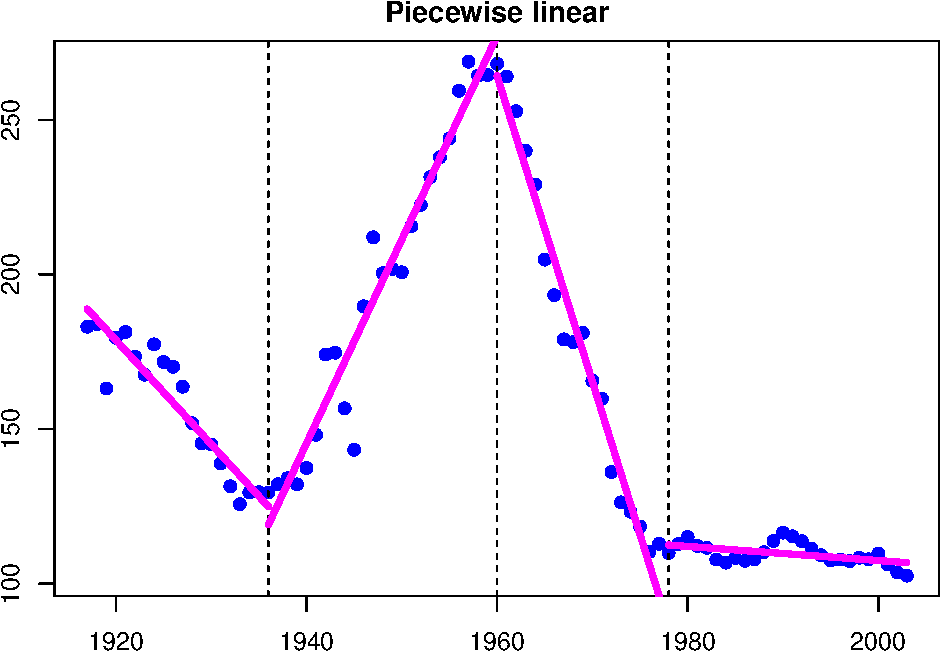
\includegraphics[keepaspectratio]{_main_files/figure-latex/unnamed-chunk-120-2.pdf}}

As we discussed in the lecture, it is a localized fit, but there are discontinuities and the overall fit is not good.

\subsubsection{Splines Regression}\label{splines-regression-1}

Instead, we can use \textbf{splines} to fit the data. Let us first try to use the B-Splines. We will first try a \textbf{linear spline}

\begin{Shaded}
\begin{Highlighting}[]
\NormalTok{bsplines.lin.fit }\OtherTok{\textless{}{-}} \FunctionTok{lm}\NormalTok{(Birthrate }\SpecialCharTok{\textasciitilde{}}\NormalTok{ splines}\SpecialCharTok{::}\FunctionTok{bs}\NormalTok{(Year, }\AttributeTok{degree =} \DecValTok{1}\NormalTok{, }\AttributeTok{knots =}\NormalTok{ myknots), }\AttributeTok{data =}\NormalTok{ birthrates)}
    \FunctionTok{plot}\NormalTok{(birthrates, }\AttributeTok{pch =} \DecValTok{19}\NormalTok{, }\AttributeTok{col =} \StringTok{"blue"}\NormalTok{)}
    \FunctionTok{lines}\NormalTok{(birthrates}\SpecialCharTok{$}\NormalTok{Year, bsplines.lin.fit}\SpecialCharTok{$}\NormalTok{fitted.values, }\AttributeTok{lty =} \DecValTok{1}\NormalTok{, }\AttributeTok{col =} \StringTok{"magenta"}\NormalTok{, }\AttributeTok{lwd =} \DecValTok{4}\NormalTok{)}
    \FunctionTok{title}\NormalTok{(}\StringTok{"Linear pline with the bs() function"}\NormalTok{)}
\end{Highlighting}
\end{Shaded}

\pandocbounded{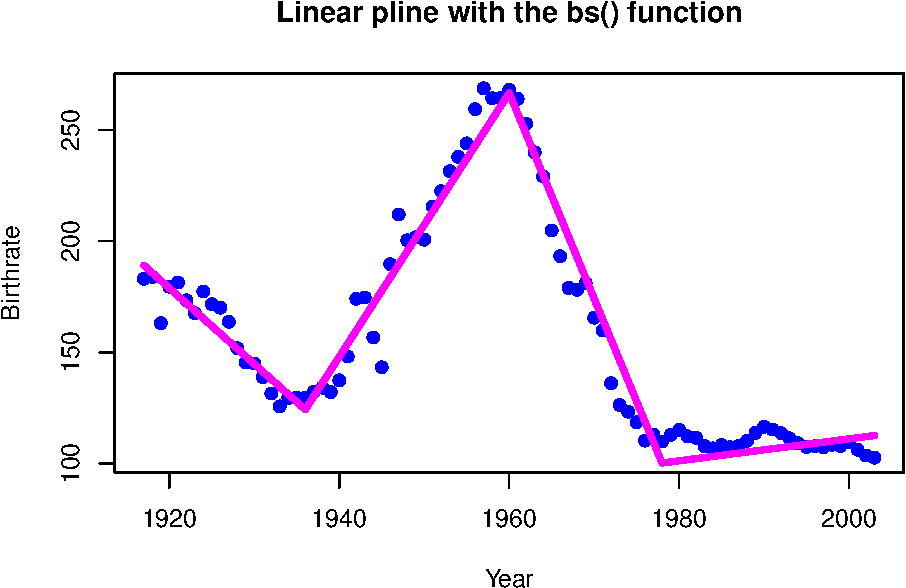
\includegraphics[keepaspectratio]{_main_files/figure-latex/unnamed-chunk-121-1.pdf}}

and then a \textbf{cubic spline} (as the ones discussed in class)

\begin{Shaded}
\begin{Highlighting}[]
\NormalTok{bsplines.}\FloatTok{3.}\NormalTok{fit }\OtherTok{\textless{}{-}} \FunctionTok{lm}\NormalTok{(Birthrate }\SpecialCharTok{\textasciitilde{}}\NormalTok{ splines}\SpecialCharTok{::}\FunctionTok{bs}\NormalTok{(Year, }\AttributeTok{degree =} \DecValTok{3}\NormalTok{, }\AttributeTok{knots =}\NormalTok{ myknots), }\AttributeTok{data =}\NormalTok{ birthrates)}
    \FunctionTok{plot}\NormalTok{(birthrates, }\AttributeTok{pch =} \DecValTok{19}\NormalTok{, }\AttributeTok{col =} \StringTok{"blue"}\NormalTok{)}
    \FunctionTok{lines}\NormalTok{(birthrates}\SpecialCharTok{$}\NormalTok{Year, bsplines.}\FloatTok{3.}\NormalTok{fit}\SpecialCharTok{$}\NormalTok{fitted.values, }\AttributeTok{lty =} \DecValTok{1}\NormalTok{, }\AttributeTok{col =} \StringTok{"magenta"}\NormalTok{, }\AttributeTok{lwd =} \DecValTok{4}\NormalTok{)}
    \FunctionTok{title}\NormalTok{(}\StringTok{"Cubic spline with 3 knots"}\NormalTok{)}
\end{Highlighting}
\end{Shaded}

\pandocbounded{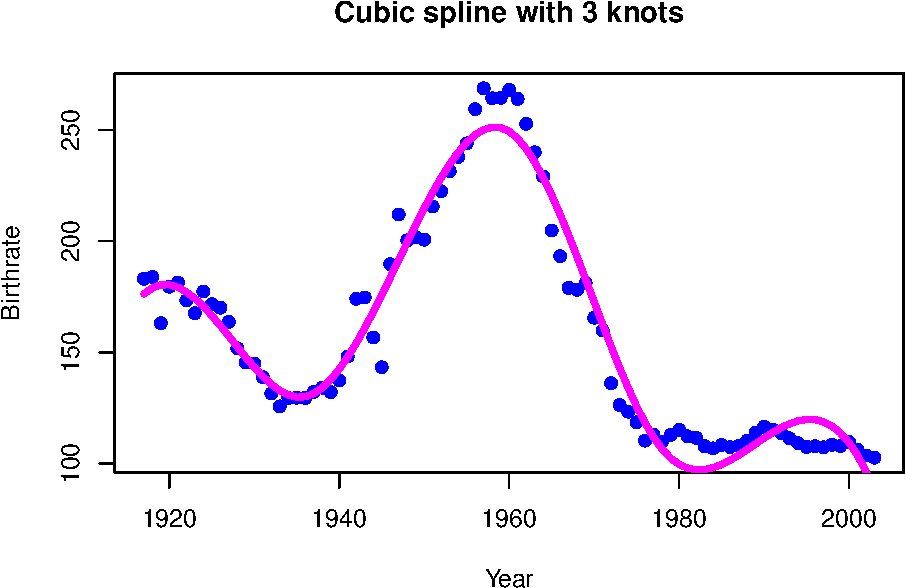
\includegraphics[keepaspectratio]{_main_files/figure-latex/unnamed-chunk-122-1.pdf}}

In the plot below, we used our pre-defined knots. We can alternatively determine the degrees of freedom in the function \texttt{bs}:

\begin{Shaded}
\begin{Highlighting}[]
\NormalTok{bsplines.}\FloatTok{3.}\NormalTok{fit.new }\OtherTok{\textless{}{-}} \FunctionTok{lm}\NormalTok{(Birthrate }\SpecialCharTok{\textasciitilde{}}\NormalTok{ splines}\SpecialCharTok{::}\FunctionTok{bs}\NormalTok{(Year, }\AttributeTok{df =} \DecValTok{5}\NormalTok{), }\AttributeTok{data =}\NormalTok{ birthrates)}
    \FunctionTok{plot}\NormalTok{(birthrates, }\AttributeTok{pch =} \DecValTok{19}\NormalTok{, }\AttributeTok{col =} \StringTok{"blue"}\NormalTok{)}
    \FunctionTok{lines}\NormalTok{(birthrates}\SpecialCharTok{$}\NormalTok{Year, bsplines.}\FloatTok{3.}\NormalTok{fit.new}\SpecialCharTok{$}\NormalTok{fitted.values, }\AttributeTok{lty =} \DecValTok{1}\NormalTok{, }\AttributeTok{col =} \StringTok{"magenta"}\NormalTok{, }\AttributeTok{lwd =} \DecValTok{4}\NormalTok{)}
    \FunctionTok{title}\NormalTok{(}\StringTok{"Cubic spline with 6 degrees of parameters"}\NormalTok{)}
\end{Highlighting}
\end{Shaded}

\pandocbounded{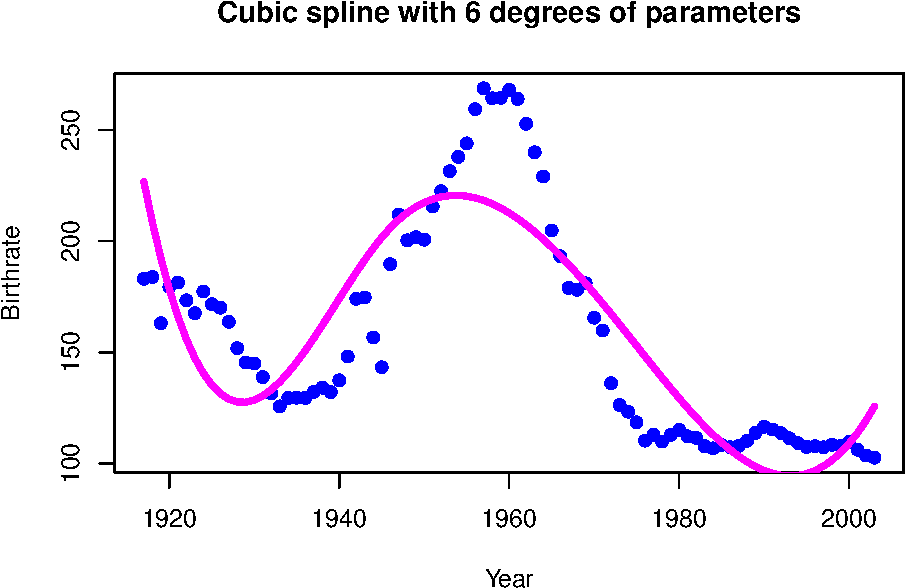
\includegraphics[keepaspectratio]{_main_files/figure-latex/unnamed-chunk-123-1.pdf}}

Let us now try the \textbf{Natural Cubic Splines}

\begin{Shaded}
\begin{Highlighting}[]
\FunctionTok{library}\NormalTok{(splines)}
\NormalTok{    ns.splines.fit }\OtherTok{=} \FunctionTok{lm}\NormalTok{(Birthrate }\SpecialCharTok{\textasciitilde{}} \FunctionTok{ns}\NormalTok{(Year, }\AttributeTok{df=}\DecValTok{6}\NormalTok{), }\AttributeTok{data=}\NormalTok{birthrates)    }
    \FunctionTok{plot}\NormalTok{(birthrates, }\AttributeTok{pch =} \DecValTok{19}\NormalTok{, }\AttributeTok{col =} \StringTok{"blue"}\NormalTok{)}
    \FunctionTok{lines}\NormalTok{(birthrates}\SpecialCharTok{$}\NormalTok{Year, ns.splines.fit}\SpecialCharTok{$}\NormalTok{fitted.values, }\AttributeTok{lty =} \DecValTok{1}\NormalTok{, }\AttributeTok{col =} \StringTok{"magenta"}\NormalTok{, }\AttributeTok{lwd =} \DecValTok{4}\NormalTok{)}
    \FunctionTok{title}\NormalTok{(}\StringTok{"Natural Cubic Splines with df=6"}\NormalTok{)}
\end{Highlighting}
\end{Shaded}

\pandocbounded{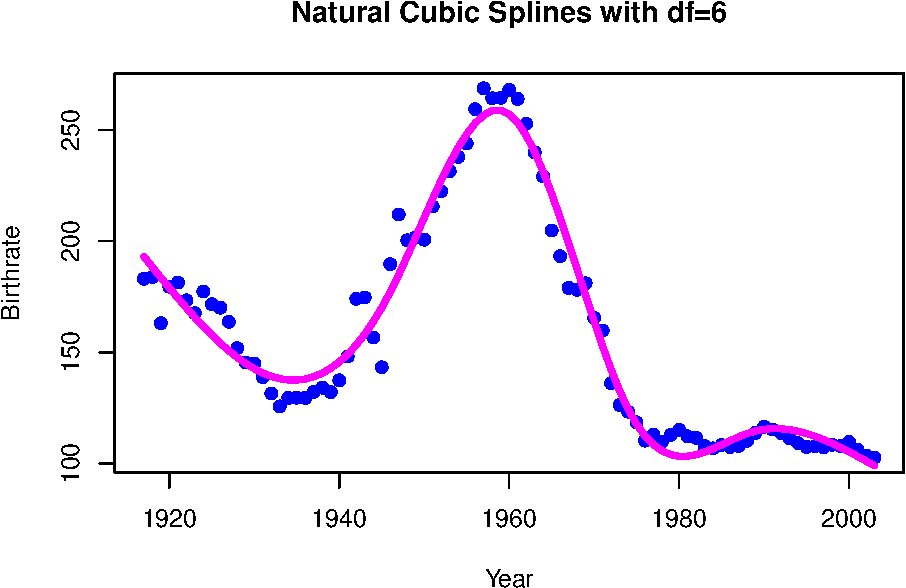
\includegraphics[keepaspectratio]{_main_files/figure-latex/unnamed-chunk-124-1.pdf}}

\subsubsection{A Simulated Example of Smoothing Splines}\label{a-simulated-example-of-smoothing-splines}

In this example, we are going to reproduce the example from the ESL book in section 5.5.2 in which we the true function of the data is given by
\[f(x) = \frac{sin(12 (x+0.2))}{x+0.2}, \, x\in[0,1]\]

So, we are first going to simulate data from this curve:

\begin{Shaded}
\begin{Highlighting}[]
\FunctionTok{set.seed}\NormalTok{(}\DecValTok{598}\NormalTok{)}
\NormalTok{n}\OtherTok{=}\DecValTok{100}

\NormalTok{x }\OtherTok{=} \FunctionTok{sort}\NormalTok{(}\FunctionTok{runif}\NormalTok{(n))}
\NormalTok{y }\OtherTok{=} \FunctionTok{sin}\NormalTok{(}\DecValTok{12}\SpecialCharTok{*}\NormalTok{(x}\FloatTok{+0.2}\NormalTok{))}\SpecialCharTok{/}\NormalTok{(x}\FloatTok{+0.2}\NormalTok{) }\SpecialCharTok{+} \FunctionTok{rnorm}\NormalTok{(n, }\DecValTok{0}\NormalTok{, }\DecValTok{1}\NormalTok{)}

\FunctionTok{plot}\NormalTok{(x, y, }\AttributeTok{col=}\StringTok{"blue"}\NormalTok{, }\AttributeTok{pch=}\DecValTok{16}\NormalTok{ )}

\NormalTok{funf\_x }\OtherTok{=} \DecValTok{1}\SpecialCharTok{:}\DecValTok{50}\SpecialCharTok{/}\DecValTok{50}
\NormalTok{funf\_y }\OtherTok{=} \FunctionTok{sin}\NormalTok{(}\DecValTok{12}\SpecialCharTok{*}\NormalTok{(funf\_x}\FloatTok{+0.2}\NormalTok{))}\SpecialCharTok{/}\NormalTok{(funf\_x}\FloatTok{+0.2}\NormalTok{)}
\FunctionTok{lines}\NormalTok{(funf\_x, funf\_y, }\AttributeTok{col=}\DecValTok{8}\NormalTok{, }\AttributeTok{lwd=}\DecValTok{2}\NormalTok{)}
\end{Highlighting}
\end{Shaded}

\pandocbounded{\includegraphics[keepaspectratio]{_main_files/figure-latex/unnamed-chunk-125-1.pdf}}

\subsubsection{Fitting a Smoothing Spline model to the simulated data above}\label{fitting-a-smoothing-spline-model-to-the-simulated-data-above}

The function to use is \texttt{smooth.spline} and is part of the \texttt{splines} library in \texttt{R}.

\begin{Shaded}
\begin{Highlighting}[]
\FunctionTok{library}\NormalTok{(splines)}
\NormalTok{?smooth.spline}
\end{Highlighting}
\end{Shaded}

The model is fitted as follows:

\begin{Shaded}
\begin{Highlighting}[]
\NormalTok{spline.model }\OtherTok{=} \FunctionTok{smooth.spline}\NormalTok{(x, y, }\AttributeTok{df=}\DecValTok{5}\NormalTok{)}
\NormalTok{spline.model}
\end{Highlighting}
\end{Shaded}

\begin{verbatim}
## Call:
## smooth.spline(x = x, y = y, df = 5)
## 
## Smoothing Parameter  spar= 0.9616029  lambda= 0.006048723 (12 iterations)
## Equivalent Degrees of Freedom (Df): 5.000634
## Penalized Criterion (RSS): 162.0406
## GCV: 1.795488
\end{verbatim}

We can compute the fitted values as follows:

\begin{Shaded}
\begin{Highlighting}[]
\NormalTok{fitted.y }\OtherTok{=} \FunctionTok{predict}\NormalTok{(spline.model, funf\_x)}
\end{Highlighting}
\end{Shaded}

To illustrate the fit of the model, we can plot the fitted line on top of the data:

\begin{Shaded}
\begin{Highlighting}[]
\FunctionTok{plot}\NormalTok{(x,y, }\AttributeTok{xlab=}\StringTok{\textquotesingle{}x\textquotesingle{}}\NormalTok{, }\AttributeTok{ylab=}\StringTok{\textquotesingle{}y\textquotesingle{}}\NormalTok{);}
\FunctionTok{lines}\NormalTok{(funf\_x, funf\_y, }\AttributeTok{col=}\DecValTok{8}\NormalTok{, }\AttributeTok{lwd=}\FloatTok{1.5}\NormalTok{);}
\FunctionTok{lines}\NormalTok{(fitted.y,  }\AttributeTok{lty=}\DecValTok{2}\NormalTok{, }\AttributeTok{col=}\StringTok{\textquotesingle{}blue\textquotesingle{}}\NormalTok{, }\AttributeTok{lwd=}\FloatTok{1.5}\NormalTok{);}
\FunctionTok{title}\NormalTok{(}\StringTok{\textquotesingle{}df=8\textquotesingle{}}\NormalTok{);}
\end{Highlighting}
\end{Shaded}

\pandocbounded{\includegraphics[keepaspectratio]{_main_files/figure-latex/unnamed-chunk-129-1.pdf}}

The blue line is the true model, while the gray line is the fitted model with 5 degrees of freedom. As we discussed, if we change the degrees of freedom, e.g.~df=8, then the line will be more/less sensitive to the data. For example for df=8 we have

\begin{Shaded}
\begin{Highlighting}[]
\FunctionTok{plot}\NormalTok{(x,y, }\AttributeTok{xlab=}\StringTok{\textquotesingle{}x\textquotesingle{}}\NormalTok{, }\AttributeTok{ylab=}\StringTok{\textquotesingle{}y\textquotesingle{}}\NormalTok{);}
\FunctionTok{lines}\NormalTok{(funf\_x, funf\_y, }\AttributeTok{col=}\DecValTok{8}\NormalTok{, }\AttributeTok{lwd=}\FloatTok{1.5}\NormalTok{);}
\FunctionTok{lines}\NormalTok{(}\FunctionTok{predict}\NormalTok{(}\FunctionTok{smooth.spline}\NormalTok{(x, y, }\AttributeTok{df=}\DecValTok{8}\NormalTok{), funf\_x),  }\AttributeTok{lty=}\DecValTok{2}\NormalTok{, }\AttributeTok{col=}\StringTok{\textquotesingle{}blue\textquotesingle{}}\NormalTok{, }\AttributeTok{lwd=}\FloatTok{1.5}\NormalTok{);}
\FunctionTok{title}\NormalTok{(}\StringTok{\textquotesingle{}df=8\textquotesingle{}}\NormalTok{);}
\end{Highlighting}
\end{Shaded}

\pandocbounded{\includegraphics[keepaspectratio]{_main_files/figure-latex/unnamed-chunk-130-1.pdf}}

\subsubsection{Choice of Lambda}\label{choice-of-lambda}

Many R packages come with an inbuilt option for determining lambda, primarily based on leave-one-out cross-validation (LOOCV) and generalized cross-validation (GCV).

There's no need to specify lambda directly. Instead, we indicate the desired degrees of freedom (df), ranging from 0 to n.~\texttt{R} then determines the appropriate lambda. We can then consult both CV and GCV curves to decide the best lambda or df.

\begin{Shaded}
\begin{Highlighting}[]
\NormalTok{model.fit }\OtherTok{=} \FunctionTok{smooth.spline}\NormalTok{(x, y, }\AttributeTok{df=}\DecValTok{9}\NormalTok{);}
\end{Highlighting}
\end{Shaded}

When using the \texttt{smooth.spline} function with a degree of freedom set at 9, the returned value \texttt{model.fit\$df} may have a slight deviation due to rounding errors.

The leverage output is equivalent to the diagonal entries of the smoothing matrix.

\begin{Shaded}
\begin{Highlighting}[]
\NormalTok{model.fit}\SpecialCharTok{$}\NormalTok{df}
\end{Highlighting}
\end{Shaded}

\begin{verbatim}
## [1] 9.001417
\end{verbatim}

\begin{Shaded}
\begin{Highlighting}[]
\NormalTok{model.fit}\SpecialCharTok{$}\NormalTok{lev  }\CommentTok{\# leveage = diagonal entries of the smoother matrix}
\end{Highlighting}
\end{Shaded}

\begin{verbatim}
##   [1] 0.30893986 0.16530188 0.15452511 0.10279673 0.08811473 0.08173143
##   [7] 0.08148178 0.08160942 0.08169108 0.08413540 0.08441745 0.11256266
##  [13] 0.12120898 0.12602066 0.13175493 0.13750648 0.13745737 0.11875674
##  [19] 0.11154402 0.10015615 0.09976906 0.08986948 0.08508903 0.08020005
##  [25] 0.07203883 0.06701137 0.06528799 0.06497591 0.06309976 0.06147779
##  [31] 0.06087571 0.06065672 0.06070371 0.06080451 0.06105153 0.06369195
##  [37] 0.06523756 0.06573835 0.06643670 0.06911934 0.06984682 0.07231683
##  [43] 0.07347632 0.08032413 0.08330237 0.08402559 0.08427316 0.07806223
##  [49] 0.07013561 0.06947727 0.06946921 0.06948635 0.06949033 0.07114094
##  [55] 0.07177155 0.07287487 0.07400078 0.08729462 0.09996053 0.14342850
##  [61] 0.14982974 0.13605679 0.10479241 0.09474069 0.08413352 0.07762692
##  [67] 0.06748810 0.06720784 0.06346315 0.06318782 0.06301969 0.06275533
##  [73] 0.06281727 0.06333844 0.06451613 0.06999234 0.07288373 0.07423106
##  [79] 0.07646914 0.07952440 0.07869513 0.07674170 0.07634088 0.07528017
##  [85] 0.07601450 0.07640336 0.07689899 0.07734393 0.08037947 0.08796840
##  [91] 0.09303429 0.09391332 0.09611884 0.10022513 0.10988799 0.12007621
##  [97] 0.13650369 0.15233032 0.15631587 0.17386379
\end{verbatim}

\begin{Shaded}
\begin{Highlighting}[]
\FunctionTok{sum}\NormalTok{(model.fit}\SpecialCharTok{$}\NormalTok{lev)}
\end{Highlighting}
\end{Shaded}

\begin{verbatim}
## [1] 9.001417
\end{verbatim}

By default, the function offers a GCV score, but you can alter it to LOOCV for comparison.

\begin{Shaded}
\begin{Highlighting}[]
\NormalTok{model.fit}\SpecialCharTok{$}\NormalTok{cv  }\CommentTok{\# default: GCV}
\end{Highlighting}
\end{Shaded}

\begin{verbatim}
## [1] FALSE
\end{verbatim}

\begin{Shaded}
\begin{Highlighting}[]
\FunctionTok{sum}\NormalTok{((y}\SpecialCharTok{{-}}\NormalTok{model.fit}\SpecialCharTok{$}\NormalTok{y)}\SpecialCharTok{\^{}}\DecValTok{2}\NormalTok{)}\SpecialCharTok{/}\NormalTok{(}\DecValTok{1}\SpecialCharTok{{-}}\NormalTok{model.fit}\SpecialCharTok{$}\NormalTok{df}\SpecialCharTok{/}\NormalTok{n)}\SpecialCharTok{\^{}}\DecValTok{2}\SpecialCharTok{/}\NormalTok{n}
\end{Highlighting}
\end{Shaded}

\begin{verbatim}
## [1] 1.577447
\end{verbatim}

\begin{Shaded}
\begin{Highlighting}[]
\NormalTok{fit}\OtherTok{=}\FunctionTok{smooth.spline}\NormalTok{(x, y, }\AttributeTok{df=}\DecValTok{9}\NormalTok{, }\AttributeTok{cv=}\NormalTok{T) }\CommentTok{\# set \textquotesingle{}cv=T\textquotesingle{} to return CV }
\NormalTok{fit}\SpecialCharTok{$}\NormalTok{cv}
\end{Highlighting}
\end{Shaded}

\begin{verbatim}
## [1] TRUE
\end{verbatim}

\begin{Shaded}
\begin{Highlighting}[]
\FunctionTok{sum}\NormalTok{(((y}\SpecialCharTok{{-}}\NormalTok{fit}\SpecialCharTok{$}\NormalTok{y)}\SpecialCharTok{/}\NormalTok{(}\DecValTok{1}\SpecialCharTok{{-}}\NormalTok{fit}\SpecialCharTok{$}\NormalTok{lev))}\SpecialCharTok{\^{}}\DecValTok{2}\NormalTok{)}\SpecialCharTok{/}\NormalTok{n}
\end{Highlighting}
\end{Shaded}

\begin{verbatim}
## [1] 1.58123
\end{verbatim}

  \bibliography{book.bib,packages.bib}

\end{document}
